\documentclass[twoside]{book}

% Packages required by doxygen
\usepackage{calc}
\usepackage{doxygen}
\usepackage{graphicx}
\usepackage[utf8]{inputenc}
\usepackage{makeidx}
\usepackage{multicol}
\usepackage{multirow}
\usepackage{textcomp}
\usepackage[table]{xcolor}

% Font selection
\usepackage[T1]{fontenc}
\usepackage{mathptmx}
\usepackage[scaled=.90]{helvet}
\usepackage{courier}
\usepackage{amssymb}
\usepackage{sectsty}
\renewcommand{\familydefault}{\sfdefault}
\allsectionsfont{%
  \fontseries{bc}\selectfont%
  \color{darkgray}%
}
\renewcommand{\DoxyLabelFont}{%
  \fontseries{bc}\selectfont%
  \color{darkgray}%
}

% Page & text layout
\usepackage{geometry}
\geometry{%
  a4paper,%
  top=2.5cm,%
  bottom=2.5cm,%
  left=2.5cm,%
  right=2.5cm%
}
\tolerance=750
\hfuzz=15pt
\hbadness=750
\setlength{\emergencystretch}{15pt}
\setlength{\parindent}{0cm}
\setlength{\parskip}{0.2cm}
\makeatletter
\renewcommand{\paragraph}{%
  \@startsection{paragraph}{4}{0ex}{-1.0ex}{1.0ex}{%
    \normalfont\normalsize\bfseries\SS@parafont%
  }%
}
\renewcommand{\subparagraph}{%
  \@startsection{subparagraph}{5}{0ex}{-1.0ex}{1.0ex}{%
    \normalfont\normalsize\bfseries\SS@subparafont%
  }%
}
\makeatother

% Headers & footers
\usepackage{fancyhdr}
\pagestyle{fancyplain}
\fancyhead[LE]{\fancyplain{}{\bfseries\thepage}}
\fancyhead[CE]{\fancyplain{}{}}
\fancyhead[RE]{\fancyplain{}{\bfseries\leftmark}}
\fancyhead[LO]{\fancyplain{}{\bfseries\rightmark}}
\fancyhead[CO]{\fancyplain{}{}}
\fancyhead[RO]{\fancyplain{}{\bfseries\thepage}}
\fancyfoot[LE]{\fancyplain{}{}}
\fancyfoot[CE]{\fancyplain{}{}}
\fancyfoot[RE]{\fancyplain{}{\bfseries\scriptsize Generated on Fri Nov 24 2023 14\-:50\-:46 for C\-A\-L\-I\-C\-E\-\_\-\-S\-I\-M by Doxygen }}
\fancyfoot[LO]{\fancyplain{}{\bfseries\scriptsize Generated on Fri Nov 24 2023 14\-:50\-:46 for C\-A\-L\-I\-C\-E\-\_\-\-S\-I\-M by Doxygen }}
\fancyfoot[CO]{\fancyplain{}{}}
\fancyfoot[RO]{\fancyplain{}{}}
\renewcommand{\footrulewidth}{0.4pt}
\renewcommand{\chaptermark}[1]{%
  \markboth{#1}{}%
}
\renewcommand{\sectionmark}[1]{%
  \markright{\thesection\ #1}%
}

% Indices & bibliography
\usepackage{natbib}
\usepackage[titles]{tocloft}
\setcounter{tocdepth}{3}
\setcounter{secnumdepth}{5}
\makeindex

% Custom commands
\newcommand{\clearemptydoublepage}{%
  \newpage{\pagestyle{empty}\cleardoublepage}%
}


%===== C O N T E N T S =====

\begin{document}

% Titlepage & ToC
\pagenumbering{roman}
\begin{titlepage}
\vspace*{7cm}
\begin{center}%
{\Large C\-A\-L\-I\-C\-E\-\_\-\-S\-I\-M \\[1ex]\large 3.\-4.\-0 }\\
\vspace*{1cm}
{\large Generated by Doxygen 1.8.5}\\
\vspace*{0.5cm}
{\small Fri Nov 24 2023 14:50:46}\\
\end{center}
\end{titlepage}
\clearemptydoublepage
\tableofcontents
\clearemptydoublepage
\pagenumbering{arabic}

%--- Begin generated contents ---
\chapter{$<$a$>$ C\-A\-L\-I\-C\-E S\-I\-M Documentation$<$/a$>$ (v01-\/00)}
\label{index}This package contains the interface classes need to analyse the lcio files which are produced out\par
 of the calice native raw data. In addition it contains the data type classes for the \par
 calice conditions data. The library being produced out of the sources has to be\par
 linked to the analysis applications. \par
 Versions of other packages to build the library\-:\par
 \par
 lcio v01-\/08 (or higher)\par
 marlin v00-\/09-\/07 (or higher)\par
 -\/--- In case database accesses (conditions data) are needed ---\par
 lccd v00-\/03 (or higher, v00-\/03-\/05 recommended)\par
 Cond\-D\-B\-My\-S\-Q\-L\-Lisbon-\/0-\/5-\/6 (or higher, Cond\-D\-B\-My\-S\-Q\-L\-\_\-\-I\-L\-C-\/0-\/5-\/10 recommended, available in calice cvs repository)\par
 -\/-\/-\/-\/-\/-\/-\/-\/-\/-\/-\/-\/-\/-\/-\/-\/-\/-\/-\/-\/-\/-\/-\/-\/-\/-\/-\/-\/-\/-\/-\/-\/-\/-\/-\/-\/-\/-\/-\/-\/-\/-\/-\/-\/-\/-\/-\/-\/-\/-\/-\/-\/-\/-\/-\/-\/-\/-\/-\/-\/---\par
 \par
 Links to older releases (links do currently not work, to be solved!!!!)\-:\par
 \par
 {\tt v01-\/02} \par
 {\tt v02-\/00-\/pre3} \par
 {\tt v03-\/05} \par
 {\tt v03-\/05-\/01} \par
 {\tt v03-\/06} \par
 {\tt v03-\/06-\/01} \par
 {\tt v03-\/07} \par
 {\tt v04-\/01-\/01} \par
 {\tt v04-\/02} \par
 {\tt v04-\/03} \par
 {\tt v04-\/03-\/01} \par
 {\tt v04-\/04-\/02} \par
 {\tt v04-\/04-\/03} \par
 {\tt v04-\/04-\/04} \par
 {\tt v04-\/04-\/05} \par
 {\tt v04-\/05-\/01} \par
 {\tt v04-\/05-\/02} \par
 {\tt v04-\/05-\/03} \par
 {\tt v04-\/06-\/00} \par
 {\tt v04-\/06-\/01} \par
 {\tt v04-\/06-\/02} \par
 {\tt v04-\/07} \par
 {\tt v04-\/07-\/01} \par
 {\tt v04-\/07-\/02} \par
 {\tt v04-\/08} \par
 {\tt v04-\/09} \par
 {\tt v04-\/10} \par
 {\tt v04-\/10-\/mc03} \par
  Changes implemented on 30/10/10  \par

\begin{DoxyItemize}
\item Bml\-Event\-Data\-Sup -\/ New class for supplementary tdc information. \par

\item Bml\-Event\-Data -\/ Access to Bml\-Event\-Data\-Sup implemented. \par

\item Bml\-Caen\-Configuration\-Block -\/ Replaces Bml\-Caen767\-Configuration\-Block on advent of Can 1290 in 2010. \par

\item Bml\-Caen\-Readout\-Configuration\-Block -\/ typedef to existing Bml\-Caen767\-Readout\-Configuration\-Block (identical for 767 and 1290 T\-D\-C). \par

\item Trigger\-Handler\-Calice -\/ Fe\-Configuration changes include and minor bug fixes. \par

\item collection\-\_\-names -\/ Generic Caen T\-D\-C collection names added plus a collection name for supplementary information. Names for handling 767 Caen T\-D\-C kept for backward compatibility.\par

\end{DoxyItemize}

Changes implemented on 7/12/10  \par

\begin{DoxyItemize}
\item Acquisition\-Data -\/ Dif counter implemented and restructuration after bug fixes in converter. \par

\item collection\-\_\-names -\/ New collection C\-O\-L\-\_\-\-D\-I\-F\-T\-R\-I\-G\-G\-E\-R.\par

\item Error\-Bits -\/ New error bit k\-Corrupt\-Dif\-Trig\-Counter, bool corrupt\-Dif\-Trig\-Counter() \par
  Changes implemented on 22/1/11  \par

\item Dhc\-Raw\-Chip\-Content\-: New interface classe for dhcal raw data
\item collection\-\_\-names -\/ Collection names for dhc data added (raw and conditions data)  Changes implemented on 12/5/11  \par

\item Dhc\-Raw\-Chip\-Content\-: returns now the Ver\-Sum
\item Dhc\-Readout\-Conf\-Block\-: New class which is the interface class to the Dhc\-Readout\-Configuration\-Data
\item collection\-\_\-names -\/ Collection name C\-O\-L\-\_\-\-D\-H\-C\-R\-O\-\_\-\-C\-O\-N\-F for Dhc\-Readoutconfiguration\-Data  Changes implemented on 03/06/11  \par

\item Trigger\-Bits, Trigger\-Handler\-Calice\-: Preparation for cern 2011 whcal running. 
\end{DoxyItemize}
\chapter{Namespace Index}
\section{Namespace List}
Here is a list of all documented namespaces with brief descriptions\-:\begin{DoxyCompactList}
\item\contentsline{section}{{\bf calice} }{\pageref{namespacecalice}}{}
\end{DoxyCompactList}

\chapter{Hierarchical Index}
\section{Class Hierarchy}
This inheritance list is sorted roughly, but not completely, alphabetically\-:\begin{DoxyCompactList}
\item I\-Conditions\-Change\-Listener\begin{DoxyCompactList}
\item \contentsline{section}{C\-A\-L\-I\-C\-E\-:\-:multi\-Calibrator}{\pageref{classCALICE_1_1multiCalibrator}}{}
\end{DoxyCompactList}
\item Processor\begin{DoxyCompactList}
\item \contentsline{section}{C\-A\-L\-I\-C\-E\-:\-:multi\-Calibrator}{\pageref{classCALICE_1_1multiCalibrator}}{}
\end{DoxyCompactList}
\item T\-Object\begin{DoxyCompactList}
\item \contentsline{section}{T\-Convolution}{\pageref{classTConvolution}}{}
\end{DoxyCompactList}
\end{DoxyCompactList}

\chapter{Data Structure Index}
\section{Class List}
Here are the classes, structs, unions and interfaces with brief descriptions\-:\begin{DoxyCompactList}
\item\contentsline{section}{{\bf C\-A\-L\-I\-C\-E\-::multi\-Calibrator} \\*Processor to add P\-A\-R\-\_\-\-M\-U\-L\-T\-I to the event and calibrate the threshold }{\pageref{classCALICE_1_1multiCalibrator}}{}
\item\contentsline{section}{{\bf T\-Convolution} \\*R\-O\-O\-T class which generates the convolution of two functions }{\pageref{classTConvolution}}{}
\end{DoxyCompactList}

\chapter{Namespace Documentation}
\section{C\-A\-L\-I\-C\-E Namespace Reference}
\label{namespaceCALICE}\index{C\-A\-L\-I\-C\-E@{C\-A\-L\-I\-C\-E}}


Store strings in L\-C\-Generic\-Objects.  


\subsection*{Data Structures}
\begin{DoxyCompactItemize}
\item 
class {\bf Acquisition\-Data}
\begin{DoxyCompactList}\small\item\em Class to store acquisition data info, i.\-e. \end{DoxyCompactList}\item 
class {\bf Adc\-Block}
\begin{DoxyCompactList}\small\item\em Class for the A\-D\-C Data as acquired by the \doxyref{C\-A\-L\-I\-C\-E}{p.}{namespaceCALICE} D\-A\-Q. \end{DoxyCompactList}\item 
class {\bf Ahc2\-Calibrations}
\begin{DoxyCompactList}\small\item\em storing all informations necessary to calibrate a H\-B\-U Si\-P\-M read channel \end{DoxyCompactList}\item 
class {\bf Ahc2\-Calibration\-Status\-Bits}
\begin{DoxyCompactList}\small\item\em Bit set to describe the Ahc2 Calibration Status. \end{DoxyCompactList}\item 
class {\bf Ahc2\-Hardware\-Connection}
\begin{DoxyCompactList}\small\item\em Class to store int values for Hardware\-Connection plus integer cell index in L\-C\-I\-O. \end{DoxyCompactList}\item 
class {\bf Ahc2\-Sat\-Corr}
\item 
class {\bf Ahc2\-Tile\-Index}
\begin{DoxyCompactList}\small\item\em Encodes/decodes hardware channel information for the Large \doxyref{C\-A\-L\-I\-C\-E}{p.}{namespaceCALICE} A\-H\-C\-A\-L prototype. \end{DoxyCompactList}\item 
class {\bf Ahc\-Amplitude}
\item 
class {\bf Ahc\-Cern2010\-Temp\-Provider}
\begin{DoxyCompactList}\small\item\em This is a temperature provider for the A\-H\-C\-A\-L.\-based on the studies of the temperature profiles from C\-E\-R\-N 2010 data. \end{DoxyCompactList}\item 
class {\bf Ahc\-Conditions}
\begin{DoxyCompactList}\small\item\em Class for the \doxyref{C\-A\-L\-I\-C\-E}{p.}{namespaceCALICE} Ahcal conditions information during the reconstruction. \end{DoxyCompactList}\item 
class {\bf Ahc\-Median\-Filter\-Temp\-Provider}
\begin{DoxyCompactList}\small\item\em This is a very simple temperature provider for the ahcal. \end{DoxyCompactList}\item 
class {\bf Ahc\-Simple\-Temp\-Provider}
\begin{DoxyCompactList}\small\item\em This is a very simple temperature provider for the ahcal. \end{DoxyCompactList}\item 
class {\bf Ahc\-Slow\-Readout\-Block}
\begin{DoxyCompactList}\small\item\em Interface Class to access the Ahc\-Slow\-Configuration Data For the time being we treat only the movable stage positions Update\-: 6/7/08 Added z and rotated position of stage (Maintain backward compatibility) \end{DoxyCompactList}\item 
class {\bf Ahc\-Slow\-Readout\-Mod\-Block}
\begin{DoxyCompactList}\small\item\em Interface Class to access the Ahc\-Slow\-Readout Data Here we handle ahc voltages, temperatures et al. \end{DoxyCompactList}\item 
class {\bf Ahc\-Slow\-Readout\-Mod\-Mapper}
\begin{DoxyCompactList}\small\item\em Class to correct the mapping of Ahc\-Slow\-Readout\-Mod\-Block-\/classes. \end{DoxyCompactList}\item 
class {\bf Ahc\-Slow\-Readout\-Mod\-Mapping}
\begin{DoxyCompactList}\small\item\em Class to store the mapping corrections for the \doxyref{Ahc\-Slow\-Readout\-Mod\-Block}{p.}{classCALICE_1_1AhcSlowReadoutModBlock}. \end{DoxyCompactList}\item 
class {\bf Ahc\-Temp\-Provider}
\begin{DoxyCompactList}\small\item\em This is an abstract class defining an interface to access the temperatures in single A\-H\-C\-A\-L cells. \end{DoxyCompactList}\item 
class {\bf Ahc\-Temp\-Sensor\-Index}
\begin{DoxyCompactList}\small\item\em \doxyref{Ahc\-Temp\-Sensor\-Index}{p.}{classCALICE_1_1AhcTempSensorIndex} represents and Ahcal Temperature Sensor Index So what? it encodes (modules,sensor) into an integer. \end{DoxyCompactList}\item 
class {\bf Ahc\-Vfe\-Configuration\-Block}
\begin{DoxyCompactList}\small\item\em Interface Class to access the Ahc\-Vfe\-Configuration\-Data. \end{DoxyCompactList}\item 
class {\bf Alignment}
\begin{DoxyCompactList}\small\item\em Class to comunicate/handle the translation into unique layer/cell ids and 3\-D spacial coordinates. \end{DoxyCompactList}\item 
class {\bf Beam\-Meta\-Data}
\item 
class {\bf Beam\-Momentum}
\begin{DoxyCompactList}\small\item\em Class to claculate the beam momentum and momentum spread from beamline slow readout data. \end{DoxyCompactList}\item 
class {\bf Beam\-Momentum\-Exception}
\begin{DoxyCompactList}\small\item\em excpetion during beam momentum calculation \end{DoxyCompactList}\item 
class {\bf Beam\-Parameter}
\begin{DoxyCompactList}\small\item\em Define the experimental setup\-: beam energy, position, angle and detector position, angle. \end{DoxyCompactList}\item 
class {\bf Beam\-Parameter\-Exception}
\begin{DoxyCompactList}\small\item\em This class handles beam parameters which have been written by hand into the database. \end{DoxyCompactList}\item 
class {\bf Be\-Event}
\begin{DoxyCompactList}\small\item\em Stores the trigger history (i.\-e. \end{DoxyCompactList}\item 
class {\bf Be\-Trg\-Conf}
\begin{DoxyCompactList}\small\item\em Stores the configuration data of the trigger. \end{DoxyCompactList}\item 
class {\bf Be\-Trg\-Event}
\begin{DoxyCompactList}\small\item\em Stores the trigger event data. \end{DoxyCompactList}\item 
class {\bf Be\-Trg\-Poll\-Data}
\begin{DoxyCompactList}\small\item\em Class to store info on trigger polling, This is useful to detect a softtrigger among e.\-g. \end{DoxyCompactList}\item 
class {\bf Binned\-Vector}
\begin{DoxyCompactList}\small\item\em Template class to store data via a linear binned keys. \end{DoxyCompactList}\item 
class {\bf Bit\-Set}
\begin{DoxyCompactList}\small\item\em Base class for easy definition of bit sets. \end{DoxyCompactList}\item 
class {\bf Bml\-Caen1290\-Configuration\-Block}
\item 
class {\bf Bml\-Caen767\-Configuration\-Block}
\begin{DoxyCompactList}\small\item\em Class to store configuration data of the 767 Caen T\-D\-C obsolete as of 31/10/10, replaced by \doxyref{Bml\-Caen\-Configuration\-Block}{p.}{classCALICE_1_1BmlCaenConfigurationBlock}, kept for backward compatibility of the code. \end{DoxyCompactList}\item 
class {\bf Bml\-Caen767\-Readout\-Configuration\-Block}
\begin{DoxyCompactList}\small\item\em Stores the configuration of the Caen767 T\-D\-C into the database At the moment I am writing this class I don't know whether they'll serve for something but it is a small uncomplicated class, so here we go. \end{DoxyCompactList}\item 
class {\bf Bml\-Caen\-Configuration\-Block}
\begin{DoxyCompactList}\small\item\em Class to store configuration data of the Caen T\-D\-Cs (767, 1290) Replaces Bml\-Caen767\-Configuration\-Data. \end{DoxyCompactList}\item 
class {\bf Bml\-Event\-Data}
\begin{DoxyCompactList}\small\item\em Class to store the \doxyref{Bml\-Event\-Data}{p.}{classCALICE_1_1BmlEventData}. \end{DoxyCompactList}\item 
class {\bf Bml\-Event\-Data\-Sup}
\begin{DoxyCompactList}\small\item\em Class to store supplementary \doxyref{Bml\-Event\-Data}{p.}{classCALICE_1_1BmlEventData}. \end{DoxyCompactList}\item 
class {\bf Bml\-Slow\-Run\-Data\-Block}
\begin{DoxyCompactList}\small\item\em Interface Class to access the Bml\-Slow\-Run Data Here we handle ahc voltages, temperatures et al. \end{DoxyCompactList}\item 
class {\bf Board\-I\-D}
\begin{DoxyCompactList}\small\item\em Create a packed board id of crate, slot, component numbers and the label. \end{DoxyCompactList}\item 
class {\bf Calibration\-Writer}
\begin{DoxyCompactList}\small\item\em Class which handles the module wise storage of conditions data and the access to the lccd framework (i.\-e. \end{DoxyCompactList}\item 
class {\bf Calice\-Conditions}
\begin{DoxyCompactList}\small\item\em Class for the \doxyref{C\-A\-L\-I\-C\-E}{p.}{namespaceCALICE} Ahcal conditions information during the reconstruction. \end{DoxyCompactList}\item 
class {\bf Calice\-Elog\-Info}
\begin{DoxyCompactList}\small\item\em Implementation of the e-\/log information. \end{DoxyCompactList}\item 
class {\bf Wrong\-Data\-Format\-Exception}
\begin{DoxyCompactList}\small\item\em exception to be thrown when the data type in a parameter is wrong \end{DoxyCompactList}\item 
class {\bf Bad\-Data\-Exception}
\begin{DoxyCompactList}\small\item\em exception to be thrown when data leads to a conflict \end{DoxyCompactList}\item 
class {\bf Calice\-Hit}
\begin{DoxyCompactList}\small\item\em Class for the \doxyref{C\-A\-L\-I\-C\-E}{p.}{namespaceCALICE} Hcal calorimeter hit information during the reconstruction. \end{DoxyCompactList}\item 
class {\bf Cell\-Index}
\begin{DoxyCompactList}\small\item\em The Mokka conform cell index. \end{DoxyCompactList}\item 
class {\bf Cell\-Mapping\-Hcal}
\begin{DoxyCompactList}\small\item\em Example for a simple mapping class based on the L\-C\-Fixed\-Object template. \end{DoxyCompactList}\item 
class {\bf Cell\-Quality}
\begin{DoxyCompactList}\small\item\em L\-C\-I\-O contions data class to describe the cell quality. \end{DoxyCompactList}\item 
class {\bf Cluster\-Shapes\-Typed}
\item 
class {\bf Conditions\-Change\-Delegator}
\begin{DoxyCompactList}\small\item\em Listens for conditions data changes and delegates the information to a class. \end{DoxyCompactList}\item 
class {\bf Conditions\-Data\-Write\-Handler}
\begin{DoxyCompactList}\small\item\em Handler of conditions data changes which writes the replaced collections to a conditions data base. \end{DoxyCompactList}\item 
class {\bf Conn\-Cell\-Mapping\-Hcal}
\begin{DoxyCompactList}\small\item\em Mapping class based on the L\-C\-Fixed\-Object template. \end{DoxyCompactList}\item 
class {\bf D\-A\-Qconnection}
\begin{DoxyCompactList}\small\item\em Class to store the D\-A\-Q address of a singel channel. \end{DoxyCompactList}\item 
class {\bf Daq\-Run\-Summary\-Block}
\begin{DoxyCompactList}\small\item\em Stores a summary of a run in terms of Number of Congfiuration Changes, Slow Readouts, Acquisitions and Number of Events in additions it stores the time of a run and for convenience the run number. \end{DoxyCompactList}\item 
class {\bf Daq\-Type\-Data\-Block}
\begin{DoxyCompactList}\small\item\em Base Class to handle all daq types (for the time being apart from the actual crc data) This base class constains the functions to store the data The actual handling of the data is left to dedicated classes which have to derive from this class. \end{DoxyCompactList}\item 
class {\bf D\-C\-Index}
\item 
class {\bf Dead\-Noise\-Constants}
\begin{DoxyCompactList}\small\item\em Class to store the results of a selection of dead or noisy cells for a certain chip/channel for a fixed module\-I\-D. \end{DoxyCompactList}\item 
class {\bf Detector\-Transformation}
\begin{DoxyCompactList}\small\item\em Define the experimental setup\-: beam energy, position, angle and detector position, angle. \end{DoxyCompactList}\item 
class {\bf Dhc\-Raw\-Chip\-Content}
\begin{DoxyCompactList}\small\item\em Simple class which stores the dhcal chip content Note that the dchal as it is now delivers the same time stamp for {\itshape all} 64 channels served by a chip. \end{DoxyCompactList}\item 
class {\bf Dhc\-Readout\-Conf\-Block}
\begin{DoxyCompactList}\small\item\em Class to interface the configuration of the Dhcal fes. \end{DoxyCompactList}\item 
class {\bf Dif\-Trigger}
\begin{DoxyCompactList}\small\item\em Simple class which stores the trigger counter retrieved from the D\-I\-F cards. \end{DoxyCompactList}\item 
class {\bf Drift\-Chamber\-Parameter}
\begin{DoxyCompactList}\small\item\em Parameters for one drift chamber. \end{DoxyCompactList}\item 
class {\bf Ecal\-Module\-Calibration}
\begin{DoxyCompactList}\small\item\em Calibration constants for the Calice E\-C\-A\-L detector modules. \end{DoxyCompactList}\item 
class {\bf Emc\-Stage\-Data\-Block}
\begin{DoxyCompactList}\small\item\em Stores information about the Emc stage Here we need to duplicate a lot of code already written by Paul since we cannot top the 'intelligence' which is introduced already there. \end{DoxyCompactList}\item 
class {\bf Encoding\-String\-Helper}
\begin{DoxyCompactList}\small\item\em Utility class to get the field description according to an lcio Bit\-Field64. \end{DoxyCompactList}\item 
class {\bf Error\-Bits}
\begin{DoxyCompactList}\small\item\em Helper class to query or set the event errors. \end{DoxyCompactList}\item 
class {\bf E\-U\-D\-A\-Q\-Block}
\begin{DoxyCompactList}\small\item\em Class for the S\-L\-C\-I\-O E\-U\-D\-A\-Q Data as acquired by the E\-U\-D\-A\-Q system. \end{DoxyCompactList}\item 
class {\bf E\-U\-D\-A\-Q\-Temp\-Sensor\-Block}
\begin{DoxyCompactList}\small\item\em Class for the temperature sensor data as acquired by the A\-H\-C\-A\-L E\-U\-D\-A\-Q. \end{DoxyCompactList}\item 
class {\bf Event\-Header}
\begin{DoxyCompactList}\small\item\em Class to store event header info, i.\-e. \end{DoxyCompactList}\item 
class {\bf Event\-Variables}
\item 
class {\bf Experimental\-Setup}
\begin{DoxyCompactList}\small\item\em Define the experimental setup\-: beam energy, position, angle and detector position, angle. \end{DoxyCompactList}\item 
struct {\bf Fast\-Calice\-Hit\-Memory\-Pool}
\item 
class {\bf Fast\-Calice\-Hit}
\begin{DoxyCompactList}\small\item\em Using Raw\-Calorimeter\-Hits as Fast\-Calice\-Hits. \end{DoxyCompactList}\item 
class {\bf Fe\-Configuration\-Block}
\begin{DoxyCompactList}\small\item\em Stores the configuration data of the front-\/end of one C\-E\-R\-C board. \end{DoxyCompactList}\item 
class {\bf Fe\-Event}
\begin{DoxyCompactList}\small\item\em Stores the trigger history (i.\-e. \end{DoxyCompactList}\item 
class {\bf Fe\-Info}
\begin{DoxyCompactList}\small\item\em Stores the configuration data of the front-\/end of one C\-E\-R\-C board. \end{DoxyCompactList}\item 
class {\bf Fe\-Trg\-Data}
\begin{DoxyCompactList}\small\item\em Stores the trigger history (i.\-e. \end{DoxyCompactList}\item 
class {\bf Gain\-Constants}
\begin{DoxyCompactList}\small\item\em Class to store the results of a Gain calibration measurement, i.\-e. \end{DoxyCompactList}\item 
class {\bf Hcal\-Boards\-Conn}
\begin{DoxyCompactList}\small\item\em Mapping class based on the L\-C\-Fixed\-Object template. \end{DoxyCompactList}\item 
class {\bf Hcal\-Cass\-Vs\-Crc}
\begin{DoxyCompactList}\small\item\em Mapping class based on the L\-C\-Fixed\-Object template that relates hcal-\/cassette $<$-\/$>$ crc board. \end{DoxyCompactList}\item 
class {\bf Hcal\-Cell\-Index}
\begin{DoxyCompactList}\small\item\em like \doxyref{C\-A\-L\-I\-C\-E\-::\-Cell\-Index}{p.}{classCALICE_1_1CellIndex}, but with H\-C\-A\-L related funciton names \end{DoxyCompactList}\item 
class {\bf Hcal\-Module\-Index\-Reverse\-Lookup}
\begin{DoxyCompactList}\small\item\em Class to simplify the lookup geometrical index to hardware index. \end{DoxyCompactList}\item 
class {\bf Hcal\-Tile\-Index}
\begin{DoxyCompactList}\small\item\em Encodes/decodes hardware channel information for the \doxyref{C\-A\-L\-I\-C\-E}{p.}{namespaceCALICE} A\-H\-C\-A\-L prototype. \end{DoxyCompactList}\item 
class {\bf Hit\-Variables}
\item 
class {\bf Hodoscope\-Block}
\begin{DoxyCompactList}\small\item\em Class for the S\-L\-C\-I\-O hododscope as acquired by the E\-U\-D\-A\-Q system. \end{DoxyCompactList}\item 
class {\bf Hodoscope\-Event\-Data\-Block}
\begin{DoxyCompactList}\small\item\em Interface class to the (L\-A\-L) Hodoscope data. \end{DoxyCompactList}\item 
class {\bf Inter\-Constants}
\begin{DoxyCompactList}\small\item\em Class to store the results of a inter calibration measurement, i.\-e. \end{DoxyCompactList}\item 
class {\bf Labview\-Block2}
\begin{DoxyCompactList}\small\item\em Class for the Labview Data as acquired by the A\-H\-C\-A\-L Labview. \end{DoxyCompactList}\item 
class {\bf Layer\-Variables}
\item 
class {\bf L\-C\-Generic\-Object\-Impl\-Cloner}
\begin{DoxyCompactList}\small\item\em Utility class to clone a L\-C\-Generic\-Object this is needed is needed since during the writing of \doxyref{C\-A\-L\-I\-C\-E}{p.}{namespaceCALICE} conditions data a full collection has to be memorized until a new set of this datatype appears. \end{DoxyCompactList}\item 
class {\bf L\-C\-Generic\-Object\-Impl\-Ext}
\begin{DoxyCompactList}\small\item\em Extends functionality of the L\-C\-Generic\-Object\-Impl Class It simply adds a new constructor to the L\-C\-Generic\-Object Class such that we can construct an interface class around without being restricted by the L\-C\-Fixed\-Object It uses an instance of L\-C\-Generic\-Object\-Impl that holds the data, thus there is no overhead when the data is read from a database or file for copying it to some local structure (Decorator pattern). \end{DoxyCompactList}\item 
class {\bf L\-C\-Hcal\-Calibration\-Object}
\begin{DoxyCompactList}\small\item\em Object to store information about arbitrary cell wise calibration of the H\-C\-A\-L in L\-C Objects. \end{DoxyCompactList}\item 
class {\bf L\-C\-Hcal\-Calibration\-Object2\-D}
\begin{DoxyCompactList}\small\item\em The results of the calibrations done by \doxyref{L\-C\-Hcal\-Calibration\-Object2\-D}{p.}{classCALICE_1_1LCHcalCalibrationObject2D} can depend on two sets of input values (like saturation correction) \end{DoxyCompactList}\item 
class {\bf Linear\-Fit\-Compound}
\begin{DoxyCompactList}\small\item\em Class to store the constant of a linear fit within the lcio framework. \end{DoxyCompactList}\item 
class {\bf Linear\-Fit\-Constant}
\begin{DoxyCompactList}\small\item\em Class to store the constant of a linear fit within the lcio framework. \end{DoxyCompactList}\item 
class {\bf Linear\-Fit\-Result}
\begin{DoxyCompactList}\small\item\em Class to store the result of a linear fit within the lcio framework. \end{DoxyCompactList}\item 
class {\bf Linear\-Fit\-Slope}
\begin{DoxyCompactList}\small\item\em Class to store the slope of a linear fit within the lcio framework. \end{DoxyCompactList}\item 
class {\bf Mapping\-And\-Alignment}
\begin{DoxyCompactList}\small\item\em Class to comunicate/handle the translation into unique layer/cell ids and 3\-D spacial coordinates. \end{DoxyCompactList}\item 
class {\bf Merged\-Hit\-Origin}
\begin{DoxyCompactList}\small\item\em Class for indicating origin of hits in merged event. \end{DoxyCompactList}\item 
class {\bf M\-I\-P\-Constants}
\begin{DoxyCompactList}\small\item\em Class to store the results of a M\-I\-P calibration measurement, i.\-e. \end{DoxyCompactList}\item 
class {\bf Module\-Connection}
\begin{DoxyCompactList}\small\item\em Defines the electric connection of a module. \end{DoxyCompactList}\item 
class {\bf Module\-Description}
\begin{DoxyCompactList}\small\item\em Description of Calice (E\-C\-A\-L) detector modules. \end{DoxyCompactList}\item 
class {\bf Module\-Location}
\begin{DoxyCompactList}\small\item\em Define possible positions of modules. \end{DoxyCompactList}\item 
class {\bf Multiple\-Conditions\-Change\-Delegator}
\begin{DoxyCompactList}\small\item\em Listens for conditions data changes and delegates the information to a class. \end{DoxyCompactList}\item 
class {\bf N\-Vector\-\_\-t}
\begin{DoxyCompactList}\small\item\em Simple n-\/dimensional vector (size of the vector is defined at compile time) Provides methods to add and subtract vectors or multiply and divide by scalars. \end{DoxyCompactList}\item 
class {\bf Pedestal\-Constants}
\begin{DoxyCompactList}\small\item\em Class to store the results of a pedestal measurement, i.\-e. \end{DoxyCompactList}\item 
class {\bf Read\-Out\-Configuration\-Block}
\begin{DoxyCompactList}\small\item\em Stores the general readout configuration. \end{DoxyCompactList}\item 
class {\bf Run\-Location}
\begin{DoxyCompactList}\small\item\em run and the generic run type i.\-e. \end{DoxyCompactList}\item 
class {\bf Run\-Location\-Whizard}
\begin{DoxyCompactList}\small\item\em Simple interface class to retrieve information about the location of a run It accesses the runlocation folder in the database. \end{DoxyCompactList}\item 
class {\bf Run\-Offset\-Value}
\begin{DoxyCompactList}\small\item\em Class to store float value, its error, and status flag plus integer index in L\-C\-I\-O. \end{DoxyCompactList}\item 
class {\bf Run\-Time\-Conditions\-Handler}
\begin{DoxyCompactList}\small\item\em Implementation of Conditions\-Handler\-Base that can be used to propagate conditions data that were generated at runtime. \end{DoxyCompactList}\item 
class {\bf Run\-Time\-Info}
\begin{DoxyCompactList}\small\item\em Simple class which holds the start and stop times of runs. \end{DoxyCompactList}\item 
class {\bf Run\-Time\-Whizard}
\begin{DoxyCompactList}\small\item\em Simple interface class to retrieve the run start and stop times by means of the runnumber. \end{DoxyCompactList}\item 
class {\bf Sat\-Corr\-Function}
\begin{DoxyCompactList}\small\item\em interface for a function to correct (or apply) the Si\-P\-M saturation \end{DoxyCompactList}\item 
class {\bf Sat\-Corr\-Itep}
\item 
class {\bf Sat\-Corr\-Itep\-Cut\-Off}
\item 
class {\bf Saturation\-Constants}
\begin{DoxyCompactList}\small\item\em Class to store the parametrisation of the saturation curve (no error yet) for a certain chip/channel for a fixed module\-I\-D. \end{DoxyCompactList}\item 
class {\bf Saturation\-Parameters}
\begin{DoxyCompactList}\small\item\em Class to store float values for Saturation Correction Curves plus integer cell index in L\-C\-I\-O. \end{DoxyCompactList}\item 
class {\bf Sc\-E\-C\-A\-L\-Gainfit}
\item 
class {\bf Sc\-E\-C\-A\-L\-Intercalib}
\item 
class {\bf Sc\-E\-C\-A\-L\-Mapping}
\item 
class {\bf Sc\-E\-C\-A\-L\-M\-I\-Pfit}
\begin{DoxyCompactList}\small\item\em Class to store the constant of a Sc\-E\-C\-A\-L M\-I\-P fit within the lcio framework. \end{DoxyCompactList}\item 
class {\bf Sc\-E\-C\-A\-L\-Noisy\-Channel}
\item 
class {\bf Sc\-E\-C\-A\-L\-One\-Pe\-A\-D\-C}
\item 
class {\bf Sc\-E\-C\-A\-L\-Temperature}
\item 
class {\bf Sce\-Slow\-Readout\-Mod\-Block}
\begin{DoxyCompactList}\small\item\em Interface Class to access the Sce\-Slow\-Readout Data Here we handle ahc voltages, temperatures et al. \end{DoxyCompactList}\item 
class {\bf Scint\-Calo\-Slow\-Readout\-Mod\-Block}
\begin{DoxyCompactList}\small\item\em Interface Class to access the Scint\-Calo\-Slow\-Readout Data Here we handle ahc voltages, temperatures et al. \end{DoxyCompactList}\item 
class {\bf Simple\-Value}
\begin{DoxyCompactList}\small\item\em Class to store float value, its error, and status flag plus integer index in L\-C\-I\-O. \end{DoxyCompactList}\item 
class {\bf Simple\-Value\-Vector}
\item 
class {\bf Si\-P\-M\-Calibrations}
\begin{DoxyCompactList}\small\item\em storing all informations necessary to calibrate a Si\-P\-M read channel \end{DoxyCompactList}\item 
class {\bf Si\-P\-M\-Calibration\-Status\-Bits}
\begin{DoxyCompactList}\small\item\em Bit set to describe the Si\-P\-M Calibration Status. \end{DoxyCompactList}\item 
class {\bf Si\-P\-M\-Mapping\-Hcal}
\begin{DoxyCompactList}\small\item\em Mapping class based on the L\-C\-Fixed\-Object template. \end{DoxyCompactList}\item 
class {\bf Si\-P\-M\-Vol\-Corr}
\begin{DoxyCompactList}\small\item\em voltage corrections for Hcal Si\-P\-Ms \end{DoxyCompactList}\item 
class {\bf Tcmt\-Connection}
\begin{DoxyCompactList}\small\item\em Defines the electronic connection of a T\-C\-M\-T strip. \end{DoxyCompactList}\item 
class {\bf Tcmt\-Event\-Bits}
\begin{DoxyCompactList}\small\item\em Bit set to describe the type of event in the T\-C\-M\-T. \end{DoxyCompactList}\item 
class {\bf Tcmt\-Event\-Identifier}
\begin{DoxyCompactList}\small\item\em class that can identify type of event in T\-C\-M\-T \end{DoxyCompactList}\item 
struct {\bf Tcmt\-Hit\-Memory\-Pool}
\item 
class {\bf Tcmt\-Hit}
\begin{DoxyCompactList}\small\item\em Using Raw\-Calorimeter\-Hits as Tcmt\-Hits. \end{DoxyCompactList}\item 
class {\bf Tcmt\-Saturation\-Constants}
\begin{DoxyCompactList}\small\item\em Class to store the estimates for the Cpix parameters for saturation corrections of T\-C\-M\-T hits. \end{DoxyCompactList}\item 
class {\bf Tdc\-Connection}
\item 
class {\bf Tdc\-Index}
\item 
class {\bf Temp\-Gain\-Constants}
\begin{DoxyCompactList}\small\item\em = class \doxyref{Gain\-Constants}{p.}{classCALICE_1_1GainConstants} but with temperature \end{DoxyCompactList}\item 
class {\bf Tiles\-Itep}
\begin{DoxyCompactList}\small\item\em Parameters of the sipm delivered by I\-T\-E\-P. \end{DoxyCompactList}\item 
class {\bf Tiles\-Itep\-Saturation}
\begin{DoxyCompactList}\small\item\em Parameters of the sipm delivered by I\-T\-E\-P. \end{DoxyCompactList}\item 
class {\bf Tiles\-Production}
\begin{DoxyCompactList}\small\item\em Parameters of the sipm delivered by P\-R\-O\-D\-U\-C\-T\-I\-O\-N. \end{DoxyCompactList}\item 
class {\bf Trg\-Readout\-Configuration\-Block}
\begin{DoxyCompactList}\small\item\em Stores the general readout configuration. \end{DoxyCompactList}\item 
class {\bf Trigger\-Bits}
\begin{DoxyCompactList}\small\item\em A small class which allow for the easy analysis of core trigger information. \end{DoxyCompactList}\item 
class {\bf Trigger\-Check}
\begin{DoxyCompactList}\small\item\em Example for a simple class based on the L\-C\-Fixed\-Object template. \end{DoxyCompactList}\item 
class {\bf Trigger\-Handler}
\begin{DoxyCompactList}\small\item\em Base Class for the user access to trigger decisions. \end{DoxyCompactList}\item 
class {\bf Trigger\-Handler\-Calice}
\begin{DoxyCompactList}\small\item\em Implementation of \doxyref{Trigger\-Handler}{p.}{classCALICE_1_1TriggerHandler} base class for calice purposes Trigger conditions are read from a conditions data source or from the event information. \end{DoxyCompactList}\item 
class {\bf Trigger\-History}
\begin{DoxyCompactList}\small\item\em Utility class to chech the zero suppressed trigger history which will be atteched to the lcio event. \end{DoxyCompactList}\item 
class {\bf Veto\-Fraction}
\begin{DoxyCompactList}\small\item\em Class to store the fraction of events that are cut with a certain purity setting of the veto. \end{DoxyCompactList}\item 
class {\bf Veto\-Threshold}
\begin{DoxyCompactList}\small\item\em Container class to store the threshold necessary to achive a certain purity. \end{DoxyCompactList}\item 
class {\bf Ahc2\-Mapper}
\begin{DoxyCompactList}\small\item\em A\-H\-C\-A\-L implementation of \doxyref{Mapper}{p.}{classCALICE_1_1Mapper} class. \end{DoxyCompactList}\item 
class {\bf Ahc\-Mapper}
\begin{DoxyCompactList}\small\item\em A\-H\-C\-A\-L implementation of \doxyref{Mapper}{p.}{classCALICE_1_1Mapper} class. \end{DoxyCompactList}\item 
class {\bf Cell\-Iterator}
\begin{DoxyCompactList}\small\item\em iterator to run over all valid (Mokka) cell I\-Ds \end{DoxyCompactList}\item 
class {\bf Decoder\-Set}
\begin{DoxyCompactList}\small\item\em class containing decoders for the three \doxyref{C\-A\-L\-I\-C\-E}{p.}{namespaceCALICE} coordinate systems \end{DoxyCompactList}\item 
class {\bf E4\-D\-Mapper}
\begin{DoxyCompactList}\small\item\em A\-H\-C\-A\-L E\-P\-T implementation of \doxyref{Mapper}{p.}{classCALICE_1_1Mapper} class Functions to get dimensions of detector geometry. \end{DoxyCompactList}\item 
class {\bf Fast\-Decoder}
\begin{DoxyCompactList}\small\item\em decode I\-Ds with encoding string \end{DoxyCompactList}\item 
class {\bf Mapped\-Container}
\begin{DoxyCompactList}\small\item\em Container for fast access by index. \end{DoxyCompactList}\item 
class {\bf Mapper}
\begin{DoxyCompactList}\small\item\em Mapping for \doxyref{C\-A\-L\-I\-C\-E}{p.}{namespaceCALICE} detectors (currently\-: H\-C\-A\-L support only) \end{DoxyCompactList}\item 
class {\bf Cell\-Description}
\begin{DoxyCompactList}\small\item\em class to hold data describing calorimeter cells \end{DoxyCompactList}\item 
class {\bf Cell\-Description\-Generator}
\begin{DoxyCompactList}\small\item\em class that generates cell descriptions objects \end{DoxyCompactList}\item 
class {\bf Cell\-Neighbour\-Calculator}
\begin{DoxyCompactList}\small\item\em class to calculate all neighbour cells \end{DoxyCompactList}\item 
class {\bf Cell\-Neighbours}
\begin{DoxyCompactList}\small\item\em class to hold information of neighbouring cells \end{DoxyCompactList}\end{DoxyCompactItemize}
\subsection*{Typedefs}
\begin{DoxyCompactItemize}
\item 
typedef int {\bfseries Adc\-Block\-Array} [6]\label{namespaceCALICE_a9c2ce8fa65a4da129464cc32041a6cb3}

\item 
typedef \\*
{\bf Scint\-Calo\-Slow\-Measures\-Dbl\-Map\-\_\-t} {\bf Ahc\-Slow\-Measures\-Dbl\-Map\-\_\-t}\label{namespaceCALICE_ad68f41183e5fdd30d4734f409778a4fb}

\begin{DoxyCompactList}\small\item\em The map which contains the measured values of the different types. \end{DoxyCompactList}\item 
typedef \\*
Scint\-Calo\-Slow\-Measures\-Int\-Map\-\_\-t {\bfseries Ahc\-Slow\-Measures\-Int\-Map\-\_\-t}\label{namespaceCALICE_a33c319ca75aaa367d8a2281f21cedd96}

\item 
typedef \\*
Scint\-Calo\-Slow\-Measures\-Float\-Map\-\_\-t {\bfseries Ahc\-Slow\-Measures\-Float\-Map\-\_\-t}\label{namespaceCALICE_ac528aeddbe40e2f1f6e3a04bfd973762}

\item 
typedef std\-::map$<$ unsigned int, \\*
std\-::vector$<$ std\-::pair$<$ bool, \\*
int $>$ $>$ $>$ {\bfseries T\-D\-C\-Channel\-Container\-\_\-t}\label{namespaceCALICE_a302ca92d51bac18357598721ba53bd0f}

\item 
typedef std\-::map$<$ unsigned, \\*
lcio\-::\-L\-C\-Collection\-Vec $\ast$ $>$ {\bfseries Calibration\-Write\-Map}\label{namespaceCALICE_a5bc82902fb43177d37fdcac4b7301558}

\item 
typedef std\-::map$<$ std\-::string, \\*
std\-::vector$<$ double $>$ $>$ {\bf Daq\-Type\-Data\-Dbl\-Map\-\_\-t}\label{namespaceCALICE_a41d5ba3d500e67c7686d34031dfbf2b1}

\begin{DoxyCompactList}\small\item\em The map which contains the measured values of the different data types. \end{DoxyCompactList}\item 
typedef std\-::map$<$ std\-::string, \\*
std\-::vector$<$ int $>$ $>$ {\bfseries Daq\-Type\-Data\-Int\-Map\-\_\-t}\label{namespaceCALICE_a1d755621385b60375eb0ea038eaadbb4}

\item 
typedef std\-::map$<$ std\-::string, \\*
std\-::vector$<$ unsigned int $>$ $>$ {\bfseries Daq\-Type\-Data\-U\-Int\-Map\-\_\-t}\label{namespaceCALICE_a26482e6cbdaf1aa8cb6ed999c82df9a7}

\item 
typedef std\-::map$<$ std\-::string, \\*
std\-::vector$<$ float $>$ $>$ {\bfseries Daq\-Type\-Data\-Float\-Map\-\_\-t}\label{namespaceCALICE_a4b2418ca1ea2654a3995d7f9af67821a}

\item 
typedef std\-::map$<$ std\-::string, \\*
L\-C\-Time $>$ {\bf Time\-Stamp\-Map\-\_\-t}\label{namespaceCALICE_a622a50caaf0a5048c39143160d9aec6c}

\begin{DoxyCompactList}\small\item\em and for the timestamps \end{DoxyCompactList}\item 
typedef std\-::map$<$ int, int $>$ {\bfseries Hodoscope\-Hit\-Map\-\_\-t}\label{namespaceCALICE_a7985c3924f9911dfd3c420759c702b3f}

\item 
typedef std\-::map$<$ unsigned, \\*
{\bf L\-C\-Hcal\-Calibration\-Object} $\ast$ $>$ {\bfseries Hcal\-Calibration\-Module\-Map}\label{namespaceCALICE_a0398f53ce0ec7e722bb3c4a4a5cb7682}

\item 
typedef std\-::pair\\*
$<$ lcio\-::\-L\-C\-Collection \\*
$\ast$, Hcal\-Calibration\-Module\-Map $\ast$ $>$ {\bfseries Hcal\-Calibration\-Module\-Data}\label{namespaceCALICE_aa0a6e980df6754a4932b7df607bffdc9}

\item 
typedef std\-::map$<$ unsigned, \\*
{\bf L\-C\-Hcal\-Calibration\-Object2\-D} $\ast$ $>$ {\bfseries Hcal\-Calibration2\-D\-Module\-Map}\label{namespaceCALICE_ad742ec973b0e96348870f3b3007f1ae7}

\item 
typedef std\-::pair\\*
$<$ lcio\-::\-L\-C\-Collection \\*
$\ast$, Hcal\-Calibration2\-D\-Module\-Map $\ast$ $>$ {\bfseries Hcal\-Calibration2\-D\-Module\-Data}\label{namespaceCALICE_adcda0108cf9121a79c99b6a9f18fe8fd}

\item 
typedef {\bf N\-Vector\-\_\-t}$<$ Float\-\_\-t, 3 $>$ {\bf Three\-Vector\-\_\-t}\label{namespaceCALICE_a1e4d014b94fc3069ff30bdddb02b786a}

\begin{DoxyCompactList}\small\item\em A three dimensional single precision floating point vector. \end{DoxyCompactList}\item 
typedef std\-::map$<$ std\-::string, \\*
std\-::vector$<$ double $>$ $>$ {\bf Scint\-Calo\-Slow\-Measures\-Dbl\-Map\-\_\-t}\label{namespaceCALICE_a3e5e6d5badfe7d664c707772da688021}

\begin{DoxyCompactList}\small\item\em The map which contains the measured values of the different types. \end{DoxyCompactList}\item 
typedef std\-::map$<$ std\-::string, \\*
std\-::vector$<$ int $>$ $>$ {\bfseries Scint\-Calo\-Slow\-Measures\-Int\-Map\-\_\-t}\label{namespaceCALICE_ab0110564397644da0bafd2107e69e9d1}

\item 
typedef std\-::map$<$ std\-::string, \\*
std\-::vector$<$ float $>$ $>$ {\bfseries Scint\-Calo\-Slow\-Measures\-Float\-Map\-\_\-t}\label{namespaceCALICE_ad5c0256c0bb692464c18ed23d75dcd5d}

\end{DoxyCompactItemize}
\subsection*{Enumerations}
\begin{DoxyCompactItemize}
\item 
enum {\bfseries E\-Acq\-Data\-Values} \{ \\*
{\bfseries k\-Acq\-Data\-Int\-Val\-Acq\-Number\-Run}, 
{\bfseries k\-Acq\-Data\-Int\-Val\-Acq\-Number\-Conf}, 
{\bfseries k\-Acq\-Data\-Int\-Val\-Acq\-Evt\-Info}, 
{\bfseries k\-Acq\-Data\-Int\-Val\-Acq\-Time\-Inf\-Sec}, 
\\*
{\bfseries k\-Acq\-Data\-Int\-Val\-Acq\-Time\-Inf\-Mus}, 
{\bfseries k\-Acq\-Data\-Int\-Val\-Acq\-State}, 
{\bfseries k\-Acq\-Data\-Int\-Val\-Has\-Dif\-Info}, 
{\bfseries k\-Acq\-Data\-Int\-Val\-Dif\-Trigger\-Counter}, 
\\*
{\bfseries k\-Acq\-Data\-Int\-Val\-Dif\-Ndata\-Buffer\-Words}, 
{\bfseries k\-Acq\-Data\-Int\-Values}
 \}
\item 
enum {\bf Ahc\-Sro\-Dbl\-Values} \{ \\*
{\bfseries kx\-Position\-\_\-mm}, 
{\bfseries ky\-Position\-\_\-mm}, 
{\bfseries kz\-Position\-\_\-mm}, 
{\bfseries kc\-Position\-\_\-deg}, 
\\*
{\bfseries k\-Sro\-Dbl\-Values}
 \}
\begin{DoxyCompactList}\small\item\em The indices of the the stored values. \end{DoxyCompactList}\item 
enum {\bf Ahc\-Sro\-Mod\-Int\-Values} \{ {\bfseries k\-Int\-Ahc\-Sro\-Mod\-Pos\-Cmb\-Vals} =k\-Int\-Sro\-Mod\-Pos\-Cmb\-Volts+2, 
{\bfseries k\-Int\-Ahc\-Sro\-Mod\-Pos\-Hbab\-Temps} =k\-Int\-Ahc\-Sro\-Mod\-Pos\-Cmb\-Vals+2, 
{\bfseries k\-Int\-Ahc\-Sro\-Mod\-Int\-Values} =k\-Int\-Sro\-Mod\-Pos\-Hbab\-Volts+1
 \}
\begin{DoxyCompactList}\small\item\em The indices of the the stored values. \end{DoxyCompactList}\item 
enum {\bfseries Ahc\-Sro\-Mod\-Dbl\-Values} \{ {\bfseries k\-Int\-Ahc\-Sro\-Mod\-Dbl\-Values}
 \}
\item 
enum {\bfseries Ahc\-Sro\-Mod\-Float\-Values} \{ {\bfseries k\-Ahc\-Int\-Sro\-Mod\-Float\-Values}
 \}
\item 
enum {\bf Ahc\-Vfe\-Int\-Values} \{ {\bfseries k\-Int\-Val\-Vfe\-Board\-Id}, 
{\bfseries k\-Int\-Ahc\-Vfe\-Rec\-Label}, 
{\bfseries k\-Int\-Verification\-Data}, 
{\bfseries k\-Int\-Shift\-Register\-Data\-Start}
 \}
\begin{DoxyCompactList}\small\item\em The indices of the the stored values. \end{DoxyCompactList}\item 
enum {\bf E\-Beam\-Parameter\-Float\-Type} \{ \\*
{\bf k\-Beam\-Parameter\-Float\-Peak\-Energy}, 
{\bf k\-Beam\-Parameter\-Float\-Beam\-Angle\-Z\-X}, 
{\bf k\-Beam\-Parameter\-Float\-Beam\-Angle\-Z\-Y}, 
{\bf k\-Beam\-Parameter\-Float\-Beam\-Impact\-Position\-X0}, 
\\*
{\bf k\-Beam\-Parameter\-Float\-Beam\-Impact\-Position\-Y0}, 
{\bfseries k\-N\-Beam\-Parameter\-Floats}
 \}
\item 
enum {\bf E\-Beam\-Parameter\-Int\-Type} \{ {\bf k\-Beam\-Parameter\-Int\-Beam\-Type}, 
{\bfseries k\-N\-Beam\-Parameter\-Ints}
 \}
\item 
enum {\bf E\-Beam\-Parameter\-Exception\-Int\-Type} \{ {\bf k\-Beam\-Parameter\-Exception\-Int\-Beam\-Energy}, 
{\bfseries k\-N\-Beam\-Parameter\-Exception\-Ints}
 \}
\item 
enum {\bfseries E\-Be\-Event\-Int\-Values} \{ \\*
{\bfseries k\-Be\-Event\-Int\-Val\-Board\-Id}, 
{\bfseries k\-Be\-Event\-Int\-Val\-Rec\-Label}, 
{\bfseries k\-Be\-Event\-Int\-Val\-Status\-Word}, 
{\bfseries k\-Be\-Event\-Int\-Val\-L1a\-Counter}, 
\\*
{\bfseries k\-Be\-Event\-Int\-Val\-Bx\-Counter}, 
{\bfseries k\-Be\-Event\-Int\-Val\-Qdr\-Frame\-Counter}, 
{\bfseries k\-Be\-Event\-Int\-Val\-Qdr\-Data\-Counter}, 
{\bfseries k\-Be\-Event\-Int\-Val\-Total\-Frame\-Counter}, 
\\*
{\bfseries k\-N\-Be\-Event\-Int\-Values}, 
{\bfseries k\-Run\-Time\-Start\-M\-S\-B}, 
{\bfseries k\-Run\-Time\-Start\-L\-S\-B}, 
{\bfseries k\-Run\-Time\-Stop\-M\-S\-B}, 
\\*
{\bfseries k\-Run\-Time\-Stop\-L\-S\-B}, 
{\bfseries k\-N\-Run\-Time\-Int\-Values}
 \}
\item 
enum {\bf E\-Be\-Trf\-Conf\-Int\-Values} \{ \\*
{\bfseries k\-Be\-Trg\-Conf\-Int\-Val\-Board\-Id}, 
{\bfseries k\-Int\-Rec\-Label}, 
{\bfseries k\-Be\-Trg\-Conf\-Int\-Val\-Input\-Enable}, 
{\bfseries k\-Be\-Trg\-Conf\-Int\-Val\-Oscillator\-Enable}, 
\\*
{\bfseries k\-Be\-Trg\-Conf\-Int\-Val\-General\-Enable}, 
{\bfseries k\-Be\-Trg\-Conf\-Int\-Val\-Oscillation\-Period}, 
{\bfseries k\-Be\-Trg\-Conf\-Int\-Val\-Burst\-Counter}, 
{\bfseries k\-Be\-Trg\-Conf\-Int\-Val\-Configuration}, 
\\*
{\bfseries k\-Be\-Trg\-Conf\-Int\-Val\-Fifo\-Idle\-Depth}, 
{\bfseries k\-Be\-Trg\-Conf\-Int\-Val\-Busy\-Timeout}, 
{\bfseries k\-Be\-Trg\-Conf\-Int\-Val\-Burst\-Timeout}, 
{\bfseries k\-Be\-Trg\-Conf\-Int\-Val\-Ext\-Beam\-Mode}, 
\\*
{\bfseries k\-Be\-Trg\-Conf\-Int\-Val\-Input\-Invert}, 
{\bfseries k\-Be\-Trg\-Conf\-Int\-Val\-Qdr\-Config}, 
{\bfseries k\-Be\-Trg\-Conf\-Int\-Val\-Sequencer\-Control}, 
{\bfseries k\-Be\-Trg\-Conf\-Int\-Val\-And\-Enable}, 
\\*
{\bfseries k\-N\-Be\-Trg\-Conf\-Int\-Values} =k\-Be\-Trg\-Conf\-Int\-Val\-And\-Enable+\-N\-L\-E\-N\-G\-A\-N\-D
 \}
\begin{DoxyCompactList}\small\item\em The indices of all the stored values. \end{DoxyCompactList}\item 
enum {\bf E\-Be\-Trg\-Event\-Int\-Values} \{ \\*
{\bfseries k\-Be\-Trg\-Event\-Int\-Val\-Board\-Id}, 
{\bfseries k\-Be\-Trg\-Event\-Int\-Val\-Rec\-Label}, 
{\bfseries k\-Be\-Trg\-Event\-Int\-Val\-Input\-Status}, 
{\bfseries k\-Be\-Trg\-Event\-Int\-Val\-Input\-Catch}, 
\\*
{\bfseries k\-Be\-Trg\-Event\-Int\-Valprebusy\-Catch}, 
{\bfseries k\-Be\-Trg\-Event\-Int\-Valsignal\-Catch}, 
{\bfseries k\-Be\-Trg\-Event\-Int\-Valcontrol}, 
{\bfseries k\-Be\-Trg\-Event\-Int\-Val\-Initial\-Fifo\-Status}, 
\\*
{\bfseries k\-Be\-Trg\-Event\-Int\-Val\-Final\-Fifo\-Status}, 
{\bfseries k\-Be\-Trg\-Event\-Int\-Valtrigger\-Counter}, 
{\bfseries k\-Be\-Trg\-Event\-Int\-Valpre\-Busy\-Trigger\-Counter}, 
{\bfseries k\-N\-Be\-Trg\-Event\-Int\-Values}
 \}
\begin{DoxyCompactList}\small\item\em The indices of all the stored values. \end{DoxyCompactList}\item 
enum {\bf E\-Be\-Trg\-Poll\-Int\-Values} \{ \\*
{\bfseries k\-Be\-Trg\-Poll\-Board\-I\-D}, 
{\bfseries k\-Be\-Trg\-Poll\-Record\-Label}, 
{\bfseries k\-Be\-Trg\-Pollstart\-Timeymd}, 
{\bfseries k\-Be\-Trg\-Pollstart\-Timehms}, 
\\*
{\bfseries k\-Be\-Trg\-Pollstart\-Timemus}, 
{\bfseries k\-Be\-Trg\-Pollend\-Timeymd}, 
{\bfseries k\-Be\-Trg\-Pollend\-Timehms}, 
{\bfseries k\-Be\-Trg\-Pollend\-Timemus}, 
\\*
{\bfseries k\-Be\-Trg\-Pollmax\-Timesec}, 
{\bfseries k\-Be\-Trg\-Pollmax\-Timemus}, 
{\bfseries k\-Betrg\-Pollnumber\-Of\-Polls}, 
{\bfseries k\-Be\-Trg\-Poll\-Timeout}, 
\\*
{\bfseries k\-Be\-Trg\-Poll\-Int\-Values}
 \}
\begin{DoxyCompactList}\small\item\em The indices of all the stored values. \end{DoxyCompactList}\item 
enum {\bfseries E\-Bml\-Caen1290\-Int\-Values} \{ \\*
{\bfseries k\-Bml\-Caen1290\-Conf\-Board\-I\-D}, 
{\bfseries k\-Bml\-Caen1290\-Conf\-Base\-Address}, 
{\bfseries k\-Bml\-Caen1290\-Conf\-Record\-Label}, 
{\bfseries k\-Bml\-Caen1290\-Conf\-Control\-Register}, 
\\*
{\bfseries k\-Bml\-Caen1290\-Conf\-Interrupt\-Register}, 
{\bfseries k\-Bml\-Caen1290\-Conf\-Count\-Register}, 
{\bfseries k\-Bml\-Caen1290\-Conf\-Int\-Values}
 \}
\item 
enum {\bfseries E\-Bml\-Caen767\-Int\-Values} \{ \\*
{\bfseries k\-Bml\-Caen767\-Conf\-Board\-I\-D}, 
{\bfseries k\-Bml\-Caen767\-Conf\-Base\-Address}, 
{\bfseries k\-Bml\-Caen767\-Conf\-Record\-Label}, 
{\bfseries k\-Bml\-Caen767\-Conf\-Control\-Register}, 
\\*
{\bfseries k\-Bml\-Caen767\-Conf\-Interrupt\-Register}, 
{\bfseries k\-Bml\-Caen767\-Conf\-Int\-Values}, 
{\bfseries k\-Bml\-Caen767\-Ro\-Conf\-Crate\-Number}, 
{\bfseries k\-Bml\-Caen767\-Ro\-Conf\-Read\-Period}, 
\\*
{\bfseries k\-Bml\-Caen767\-Ro\-Conf\-Bool\-Col}, 
{\bfseries k\-Bml\-Caen767\-Ro\-Conf\-Mode}, 
{\bfseries k\-Bml\-Caen767\-Ro\-Conf\-Int\-Values}
 \}
\item 
enum {\bf E\-Bml\-Caen767\-Int\-Values} \{ \\*
{\bfseries k\-Bml\-Caen767\-Conf\-Board\-I\-D}, 
{\bfseries k\-Bml\-Caen767\-Conf\-Base\-Address}, 
{\bfseries k\-Bml\-Caen767\-Conf\-Record\-Label}, 
{\bfseries k\-Bml\-Caen767\-Conf\-Control\-Register}, 
\\*
{\bfseries k\-Bml\-Caen767\-Conf\-Interrupt\-Register}, 
{\bfseries k\-Bml\-Caen767\-Conf\-Int\-Values}, 
{\bfseries k\-Bml\-Caen767\-Ro\-Conf\-Crate\-Number}, 
{\bfseries k\-Bml\-Caen767\-Ro\-Conf\-Read\-Period}, 
\\*
{\bfseries k\-Bml\-Caen767\-Ro\-Conf\-Bool\-Col}, 
{\bfseries k\-Bml\-Caen767\-Ro\-Conf\-Mode}, 
{\bfseries k\-Bml\-Caen767\-Ro\-Conf\-Int\-Values}
 \}
\begin{DoxyCompactList}\small\item\em The indices of all the stored values. \end{DoxyCompactList}\item 
enum {\bfseries E\-Bml\-Caen\-Int\-Values} \{ \\*
{\bfseries k\-Bml\-Caen\-Conf\-Board\-I\-D}, 
{\bfseries k\-Bml\-Caen\-Conf\-Base\-Address}, 
{\bfseries k\-Bml\-Caen\-Conf\-Record\-Label}, 
{\bfseries k\-Bml\-Caen\-Conf\-Control\-Register}, 
\\*
{\bfseries k\-Bml\-Caen\-Conf\-Interrupt\-Register}, 
{\bfseries k\-Bml\-Caen\-Conf\-Count\-Register}, 
{\bfseries k\-Bml\-Caen\-Conf\-Spare}, 
{\bfseries k\-Bml\-Caen\-Conf\-Int\-Values}
 \}
\item 
enum {\bf E\-Bml\-Event\-Int\-Values} \{ \\*
{\bfseries k\-Bml\-Event\-Board\-I\-D}, 
{\bfseries k\-Bml\-Event\-Base\-Address}, 
{\bfseries k\-Bml\-Event\-Record\-Label}, 
{\bfseries k\-Bml\-Event\-Status\-Register}, 
\\*
{\bfseries k\-Bml\-Event\-Number\-Of\-Words}, 
{\bfseries k\-Bml\-Eventgeo\-Address}, 
{\bfseries k\-Bml\-Eventevent\-Number}, 
{\bfseries k\-Bml\-Event\-Status}, 
\\*
{\bfseries k\-Bml\-Event\-Event\-Data\-Counter}, 
{\bfseries k\-Bml\-Event\-Number\-Of\-Signal\-Channels}, 
{\bfseries k\-Bml\-Event\-Int\-Values}
 \}
\begin{DoxyCompactList}\small\item\em The indices of all the stored values. \end{DoxyCompactList}\item 
enum {\bf E\-Bml\-Event\-Sup\-Int\-Values} \{ \\*
{\bfseries k\-Bml\-Event\-Sup\-Fifo}, 
{\bfseries k\-Bml\-Event\-Sup\-Event\-I\-D\-Trailer}, 
{\bfseries k\-Bml\-Event\-Sup\-Bunch\-I\-D}, 
{\bfseries k\-Bml\-Event\-Sup\-T\-D\-C\-Errors}, 
\\*
{\bfseries k\-Bml\-Event\-Sup\-Buffer\-Overflow}, 
{\bfseries k\-Bml\-Event\-Sup\-Trigger\-Lost}, 
{\bfseries k\-Bml\-Event\-Sup\-T\-D\-C\-Word\-Count\-Trailer}, 
{\bfseries k\-Bml\-Event\-Names\-Pointer}, 
\\*
{\bfseries k\-Bml\-Event\-Names\-Length}, 
{\bfseries k\-Bml\-Event\-Sup\-Int\-Values}
 \}
\begin{DoxyCompactList}\small\item\em The indices of all the stored values. \end{DoxyCompactList}\item 
enum {\bf Bml\-Sro\-Run\-Int\-Values} \{ \\*
{\bfseries k\-Int\-Bml\-Sro\-Run\-Pos\-Time\-Stampymd}, 
{\bfseries k\-Int\-Bml\-Sro\-Run\-Pos\-Time\-Stamphms}, 
{\bfseries k\-Int\-Bml\-Sro\-Run\-Pos\-Sext\-Cur}, 
{\bfseries k\-Int\-Bml\-Sro\-Run\-Pos\-Bend\-Cur} =k\-Int\-Bml\-Sro\-Run\-Pos\-Sext\-Cur+2, 
\\*
{\bfseries k\-Int\-Bml\-Sro\-Run\-Pos\-Col\-Pos} =k\-Int\-Bml\-Sro\-Run\-Pos\-Bend\-Cur+2, 
{\bfseries k\-Int\-Bml\-Sro\-Run\-Pos\-Quad\-Cur} =k\-Int\-Bml\-Sro\-Run\-Pos\-Col\-Pos+2, 
{\bfseries k\-Int\-Bml\-Sro\-Run\-Pos\-Trim\-Cur} =k\-Int\-Bml\-Sro\-Run\-Pos\-Quad\-Cur+2, 
{\bfseries k\-Int\-Bml\-Sro\-Run\-Pos\-H6a\-Exp\-Count} =k\-Int\-Bml\-Sro\-Run\-Pos\-Trim\-Cur+2, 
\\*
{\bfseries k\-Int\-Bml\-Sro\-Run\-Pos\-H6b\-Exp\-Count} =k\-Int\-Bml\-Sro\-Run\-Pos\-H6a\-Exp\-Count+2, 
{\bfseries k\-Int\-Bml\-Sro\-Run\-Pos\-H6c\-Exp\-Count} =k\-Int\-Bml\-Sro\-Run\-Pos\-H6b\-Exp\-Count+2, 
{\bfseries k\-Int\-Bml\-Sro\-Run\-Pos\-Rp\-Exp\-Count} =k\-Int\-Bml\-Sro\-Run\-Pos\-H6c\-Exp\-Count+2, 
{\bfseries k\-Int\-Bml\-Sro\-Run\-Pos\-Scint\-Count} =k\-Int\-Bml\-Sro\-Run\-Pos\-Rp\-Exp\-Count+2, 
\\*
{\bfseries k\-Int\-Bml\-Sro\-Run\-Int\-Values}
 \}
\begin{DoxyCompactList}\small\item\em The map which contains the measured values of the different data types. \end{DoxyCompactList}\item 
enum {\bfseries Bml\-Sro\-Run\-Dbl\-Values} \{ {\bfseries k\-Dbl\-Bml\-Sro\-Run\-Pos\-Abs\-Position}, 
{\bfseries k\-Dbl\-Bml\-Sro\-Run\-Pos\-T4\-Position}, 
{\bfseries k\-Dbl\-Bml\-Sro\-Run\-Pos\-Target\-Position}, 
{\bfseries k\-Int\-Bml\-Sro\-Run\-Dbl\-Values}
 \}
\item 
enum {\bfseries Bml\-Sro\-Run\-Float\-Values} \{ {\bfseries k\-Int\-Bml\-Sro\-Run\-Float\-Values}
 \}
\item 
enum {\bf E\-Daq\-Sum\-Int\-Values} \{ \\*
{\bfseries k\-Daq\-Run\-Num}, 
{\bfseries k\-Daq\-Num\-Conf}, 
{\bfseries k\-Daq\-Num\-Sro}, 
{\bfseries k\-Daq\-Num\-Acq}, 
\\*
{\bfseries k\-Daq\-Num\-Evt}, 
{\bfseries k\-Daq\-Run\-Time}, 
{\bfseries k\-Daq\-Num\-Int\-Vals}
 \}
\begin{DoxyCompactList}\small\item\em The indices of all the stored values. \end{DoxyCompactList}\item 
enum {\bf Daq\-Type\-Int\-Values} \{ \\*
{\bfseries k\-Int\-Daq\-Type\-Time\-Stamps}, 
{\bfseries k\-Int\-Daq\-Type\-Time\-Stamp\-Names\-Pointer}, 
{\bfseries k\-Int\-Daq\-Type\-Time\-Stamp\-Names\-Length}, 
{\bfseries k\-Int\-Daq\-Type\-Int\-Types}, 
\\*
{\bfseries k\-Int\-Daq\-Type\-Dbl\-Types}, 
{\bfseries k\-Int\-Daq\-Type\-Float\-Types}, 
{\bfseries k\-Int\-Daq\-Type\-Int\-Names\-Pointer}, 
{\bfseries k\-Int\-Daq\-Type\-Dbl\-Names\-Pointer}, 
\\*
{\bfseries k\-Int\-Daq\-Type\-Float\-Names\-Pointer}, 
{\bfseries k\-Int\-Daq\-Type\-Int\-Names\-Length}, 
{\bfseries k\-Int\-Daq\-Type\-Dbl\-Names\-Length}, 
{\bfseries k\-Int\-Daq\-Type\-Float\-Names\-Length}, 
\\*
{\bfseries k\-Int\-Daq\-Type\-Int\-Sizes}, 
{\bfseries k\-Int\-Daq\-Type\-Dbl\-Sizes}, 
{\bfseries k\-Int\-Daq\-Type\-Float\-Sizes}, 
{\bfseries k\-Int\-Daq\-Type\-Data\-Start}
 \}
\begin{DoxyCompactList}\small\item\em The indices of the the stored values. \end{DoxyCompactList}\item 
enum {\bfseries Daq\-Type\-Dbl\-Values} \{ {\bfseries k\-Int\-Daq\-Type\-Dbl\-Readings}
 \}
\item 
enum {\bfseries Daq\-Type\-Float\-Values} \{ {\bfseries k\-Int\-Daq\-Type\-Float\-Readings}
 \}
\item 
enum {\bf E\-Detector\-Transformation\-Float\-Type} \{ \\*
{\bf k\-Detector\-Transformation\-Float\-Detector\-Angle\-Z\-X}, 
{\bf k\-Detector\-Transformation\-Float\-Detector\-Rotation\-X0}, 
{\bf k\-Detector\-Transformation\-Float\-Detector\-Rotation\-Z0}, 
{\bf k\-Detector\-Transformation\-Float\-Detector\-X0}, 
\\*
{\bf k\-Detector\-Transformation\-Float\-Detector\-Y0}, 
{\bf k\-Detector\-Transformation\-Float\-Detector\-Z0}, 
{\bfseries k\-N\-Detector\-Transformation\-Floats}
 \}
\item 
enum {\bfseries E\-Detector\-Transformation\-Int\-Type} \{ {\bfseries k\-N\-Detector\-Transformation\-Ints}
 \}
\item 
enum {\bfseries E\-Dhc\-Raw\-Chip\-Content\-Int\-Values} \{ \\*
{\bfseries k\-Dhc\-Raw\-Chip\-Int\-Crate\-Nr}, 
{\bfseries k\-Dhc\-Raw\-Chip\-Int\-Elec\-Adr}, 
{\bfseries k\-Dhc\-Raw\-Chip\-Int\-Hits\-Hi}, 
{\bfseries k\-Dhc\-Raw\-Chip\-Int\-Hits\-Lo}, 
\\*
{\bfseries k\-Dhc\-Raw\-Chip\-Int\-Time\-Stamp}, 
{\bfseries k\-Dhc\-Raw\-Chip\-Int\-Misc\-Info}, 
{\bfseries k\-Dhc\-Raw\-Chip\-Int\-Values}
 \}
\item 
enum {\bfseries E\-Dhcreadout\-Configuration\-Int\-Values} \{ \\*
{\bfseries k\-Dhc\-Ro\-Conf\-Int\-Numbers}, 
{\bfseries k\-Dhc\-Ro\-Conf\-Int\-Slot\-Enable\-Mask}, 
{\bfseries k\-Dhc\-Ro\-Conf\-Int\-Slot\-Enable}, 
{\bfseries k\-Dhc\-Ro\-Conf\-Int\-Num\-Slots}, 
\\*
{\bfseries k\-Dhc\-Ro\-Conf\-Int\-Be\-Time\-Dif}, 
{\bfseries k\-Dhc\-Ro\-Conf\-Int\-Values}
 \}
\item 
enum {\bfseries E\-Dif\-Trigger\-Int\-Values} \{ {\bfseries k\-Dif\-Trigger\-Counter}, 
{\bfseries k\-Dif\-Trigger\-Int\-Values}
 \}
\item 
enum {\bf E\-Drift\-Chamber\-Parameter\-Float\-Type} \{ \\*
{\bf k\-Drift\-Chamber\-Parameter\-Float\-Velocity}, 
{\bf k\-Drift\-Chamber\-Parameter\-Float\-Delay}, 
{\bf k\-Drift\-Chamber\-Parameter\-Float\-Offset\-Z}, 
{\bf k\-Drift\-Chamber\-Parameter\-Float\-Offset\-U}, 
\\*
{\bf k\-Drift\-Chamber\-Parameter\-Float\-Error}, 
{\bfseries k\-N\-Drift\-Chamber\-Parameter\-Floats}
 \}
\item 
enum {\bf E\-Drift\-Chamber\-Parameter\-Int\-Type} \{ {\bf k\-Drift\-Chamber\-Parameter\-Int\-Wire\-Type}, 
{\bfseries k\-N\-Drift\-Chamber\-Parameter\-Ints}
 \}
\item 
enum {\bfseries E\-Drift\-Chamber\-Wire\-Type} \{ \\*
{\bfseries k\-Drift\-Chamber\-Wire\-Minus}, 
{\bfseries k\-Drift\-Chamber\-Wire\-Plus}, 
{\bfseries k\-Drift\-Chamber\-Wire\-X\-Minus}, 
{\bfseries k\-Drift\-Chamber\-Wire\-X\-Plus}, 
\\*
{\bfseries k\-Drift\-Chamber\-Wire\-Y\-Minus}, 
{\bfseries k\-Drift\-Chamber\-Wire\-Y\-Plus}, 
{\bfseries k\-N\-Wire\-Types}
 \}
\item 
enum {\bfseries E\-Ecal\-Module\-Calibration\-Int\-Type} \{ {\bfseries k\-Ecal\-Module\-Calibration\-Int\-Module\-I\-D}, 
{\bfseries k\-Ecal\-Module\-Calibration\-Int\-Name\-Length}, 
{\bfseries k\-N\-Ecal\-Module\-Calibration\-Ints}
 \}
\item 
enum {\bfseries E\-Ecal\-Module\-Calibration\-Float\-Type} \{ {\bfseries k\-N\-Ecal\-Module\-Calibration\-Floats}
 \}
\item 
enum {\bf E\-Emc\-St\-Int\-Values} \{ \\*
{\bfseries k\-Emc\-St\-Header}, 
{\bfseries k\-Emc\-Stx\-Status}, 
{\bfseries k\-Emc\-Stx\-Value}, 
{\bfseries k\-Emc\-Sty\-Status} =k\-Emc\-Stx\-Value+\-N\-U\-M\-X\-V\-A\-L\-U\-E\-S, 
\\*
{\bfseries k\-Emc\-Sty\-Value}, 
{\bfseries k\-Emc\-St\-Check\-Sum} =k\-Emc\-Sty\-Value+\-N\-U\-M\-Y\-V\-A\-L\-U\-E\-S
 \}
\begin{DoxyCompactList}\small\item\em The indices of all the stored values. \end{DoxyCompactList}\item 
enum {\bf E\-Experimental\-Setup\-Float\-Type} \{ \\*
{\bf k\-Experimental\-Setup\-Float\-Peak\-Energy}, 
{\bf k\-Experimental\-Setup\-Float\-Beam\-Angle\-Z\-X}, 
{\bf k\-Experimental\-Setup\-Float\-Beam\-Angle\-Z\-Y}, 
{\bf k\-Experimental\-Setup\-Float\-Beam\-Impact\-Position\-X0}, 
\\*
{\bf k\-Experimental\-Setup\-Float\-Beam\-Impact\-Position\-Y0}, 
{\bf k\-Experimental\-Setup\-Float\-Detector\-Angle\-Z\-X}, 
{\bf k\-Experimental\-Setup\-Float\-Detector\-Rotation\-X0}, 
{\bf k\-Experimental\-Setup\-Float\-Detector\-Rotation\-Z0}, 
\\*
{\bf k\-Experimental\-Setup\-Float\-Detector\-X0}, 
{\bf k\-Experimental\-Setup\-Float\-Detector\-Y0}, 
{\bf k\-Experimental\-Setup\-Float\-Detector\-Z0}, 
{\bfseries k\-N\-Experimental\-Setup\-Floats}
 \}
\item 
enum {\bf E\-Experimental\-Setup\-Int\-Type} \{ {\bf k\-Experimental\-Setup\-Int\-Beam\-Type}, 
{\bfseries k\-N\-Experimental\-Setup\-Ints}
 \}
\item 
enum {\bf E\-Fe\-Conf\-Block\-Int\-Values} \{ \\*
{\bfseries k\-Fe\-Conf\-Block\-Int\-Val\-Fe\-Board\-Id}, 
{\bfseries k\-Int\-Fe\-Rec\-Label}, 
{\bfseries k\-Fe\-Conf\-Block\-Int\-Val\-Calib\-Start}, 
{\bfseries k\-Fe\-Conf\-Block\-Int\-Val\-Calib\-Width}, 
\\*
{\bfseries k\-Fe\-Conf\-Block\-Int\-Val\-Hold\-Start}, 
{\bfseries k\-Fe\-Conf\-Block\-Int\-Val\-Hold\-Width}, 
{\bfseries k\-Fe\-Conf\-Block\-Int\-Val\-Vfe\-Reset\-Start}, 
{\bfseries k\-Fe\-Conf\-Block\-Int\-Val\-Vfe\-Reset\-End}, 
\\*
{\bfseries k\-Fe\-Conf\-Block\-Int\-Val\-Vfe\-Srin\-Start}, 
{\bfseries k\-Fe\-Conf\-Block\-Int\-Val\-Vfe\-Srin\-End}, 
{\bfseries k\-Fe\-Conf\-Block\-Int\-Val\-Vfe\-Mplex\-Clock\-Start}, 
{\bfseries k\-Fe\-Conf\-Block\-Int\-Val\-Vfe\-Mplex\-Clock\-Mark}, 
\\*
{\bfseries k\-Fe\-Conf\-Block\-Int\-Val\-Vfe\-Mplex\-Clock\-Space}, 
{\bfseries k\-Fe\-Conf\-Block\-Int\-Val\-Vfe\-Mplex\-Clock\-Pulses}, 
{\bfseries k\-Fe\-Conf\-Block\-Int\-Val\-Adc\-Start}, 
{\bfseries k\-Fe\-Conf\-Block\-Int\-Val\-Adc\-End}, 
\\*
{\bfseries k\-Fe\-Conf\-Block\-Int\-Val\-Adc\-Control}, 
{\bfseries k\-Fe\-Conf\-Block\-Int\-Val\-Adc\-Delay}, 
{\bfseries k\-Fe\-Conf\-Block\-Int\-Val\-Frame\-Sync\-Delay}, 
{\bfseries k\-Fe\-Conf\-Block\-Int\-Val\-Qdr\-Data\-Delay}, 
\\*
{\bfseries k\-Fe\-Conf\-Block\-Int\-Val\-Dac\-Data}, 
{\bfseries k\-Fe\-Conf\-Block\-Int\-Val\-Flags}, 
{\bfseries k\-Fe\-Conf\-Block\-Int\-Val\-Vfe\-Info}, 
{\bfseries k\-Fe\-Conf\-Block\-Int\-Val\-Emc\-Bot}, 
\\*
{\bfseries k\-Fe\-Conf\-Block\-Int\-Val\-Emc\-Top}, 
{\bfseries k\-Fe\-Conf\-Block\-Int\-Val\-Emc\-Top\-Low\-Gain\-Bit}, 
{\bfseries k\-Fe\-Conf\-Block\-Int\-Val\-Emc\-Bot\-Low\-Gain\-Bit}, 
{\bfseries k\-N\-Fe\-Conf\-Block\-Int\-Values}
 \}
\begin{DoxyCompactList}\small\item\em The indices of all the stored values. \end{DoxyCompactList}\item 
enum {\bfseries E\-Fe\-Event\-Int\-Values} \{ \\*
{\bfseries k\-Fe\-Event\-Int\-Val\-Board\-Id}, 
{\bfseries k\-Fe\-Event\-Int\-Val\-Rec\-Label}, 
{\bfseries k\-Fe\-Event\-Int\-Val\-Trigger\-Counter}, 
{\bfseries k\-Fe\-Event\-Int\-Val\-Spy\-Register}, 
\\*
{\bfseries k\-N\-Fe\-Event\-Int\-Values}
 \}
\item 
enum {\bf E\-Int\-Values} \{ \\*
{\bfseries k\-Int\-Val\-Fe\-Info\-Board\-Id}, 
{\bfseries k\-Int\-Val\-Fe\-Info\-Label}, 
{\bfseries k\-Int\-Val\-Fe\-Info\-Fe\-I\-D}, 
{\bfseries k\-Int\-Val\-Fe\-Info\-Frame\-Sync\-Out\-Packed0}, 
\\*
{\bfseries k\-Int\-Val\-Fe\-Info\-Frame\-Sync\-Out\-Packed2}, 
{\bfseries k\-Int\-Val\-Fe\-Info\-Fe\-Length}, 
{\bfseries k\-Int\-Val\-Fe\-Info\-Frame\-Sync\-Out\-Packed4}, 
{\bfseries k\-Int\-Val\-Fe\-Info\-Fifo}, 
\\*
{\bfseries k\-Int\-Val\-Fe\-Info\-Trigger\-Counter}, 
{\bfseries k\-N\-Int\-Values\-Fe\-Info}
 \}
\begin{DoxyCompactList}\small\item\em The indices of all the stored values. \end{DoxyCompactList}\item 
enum {\bfseries E\-Fe\-Trg\-Data\-Int\-Values} \{ \\*
{\bfseries k\-Fe\-Trg\-Data\-Int\-Val\-Board\-Id}, 
{\bfseries k\-Fe\-Trg\-Data\-Int\-Val\-Rec\-Label}, 
{\bfseries k\-Fe\-Trg\-Data\-Int\-Val\-Header}, 
{\bfseries k\-Fe\-Trg\-Data\-Int\-Val\-Trailer}, 
\\*
{\bfseries k\-Fe\-Trg\-Data\-Int\-Val\-Trig\-Counter}, 
{\bfseries k\-N\-Fe\-Trg\-Data\-Int\-Values}
 \}
\item 
enum {\bf E\-Ro\-Conf\-Int\-Values} \{ \\*
{\bfseries k\-Hod\-Evt\-Status}, 
{\bfseries k\-Hod\-Evt\-Evt\-Counter}, 
{\bfseries k\-Hod\-Evt\-Time\-Counter}, 
{\bfseries k\-Hod\-Evt\-Num\-Hits\-X}, 
\\*
{\bfseries k\-Hod\-Evt\-Num\-Hits\-Y}, 
{\bfseries k\-Ro\-Conf\-Int\-Numbers}, 
{\bfseries k\-Ro\-Conf\-Int\-Slot\-Enable}, 
{\bfseries k\-Ro\-Conf\-Int\-Slot\-Fe\-Enable}, 
\\*
{\bfseries k\-Ro\-Conf\-Int\-Vme\-Period} =k\-Ro\-Conf\-Int\-Slot\-Fe\-Enable+\-N\-L\-E\-N\-S\-L\-O\-F\-E, 
{\bfseries k\-Ro\-Conf\-Int\-Be\-Period}, 
{\bfseries k\-Ro\-Conf\-Int\-Bec\-Period}, 
{\bfseries k\-Ro\-Conf\-Int\-Fe\-Period}, 
\\*
{\bfseries k\-Ro\-Conf\-Int\-Be\-Soft\-Trigger}, 
{\bfseries k\-Ro\-Conf\-Int\-Fe\-Soft\-Trigger}, 
{\bfseries k\-Ro\-Conf\-Int\-Fe\-Brc\-Soft\-Trigger}, 
{\bfseries k\-Ro\-Int\-Conf\-Mode}, 
\\*
{\bfseries k\-N\-Ro\-Conf\-Int\-Values} =k\-Ro\-Int\-Conf\-Mode
 \}
\begin{DoxyCompactList}\small\item\em The indices of all the stored values. \end{DoxyCompactList}\item 
enum {\bfseries E\-Int\-L\-F\-Values} \{ {\bfseries k\-\_\-\-I\-D\-\_\-\-Int\-L\-F}, 
{\bfseries k\-N\-Int\-L\-F\-Values}
 \}
\item 
enum {\bfseries E\-Float\-L\-F\-Values} \{ {\bfseries k\-N\-Float\-L\-F\-Values}
 \}
\item 
enum {\bfseries E\-Double\-L\-F\-Values} \{ \\*
{\bfseries k\-\_\-\-Constant\-\_\-\-Double\-L\-F}, 
{\bfseries k\-\_\-\-Constant\-\_\-\-Error\-\_\-\-Double\-L\-F}, 
{\bfseries k\-\_\-\-Constant\-\_\-\-Reference\-\_\-\-Point\-\_\-\-Double\-L\-F}, 
{\bfseries k\-\_\-\-Constant\-\_\-\-Reference\-\_\-\-Point\-\_\-\-Error\-\_\-\-Double\-L\-F}, 
\\*
{\bfseries k\-\_\-\-Slope\-\_\-\-Double\-L\-F}, 
{\bfseries k\-\_\-\-Slope\-\_\-\-Error\-\_\-\-Double\-L\-F}, 
{\bfseries k\-N\-Double\-L\-F\-Values}
 \}
\item 
enum {\bfseries E\-Int\-L\-F\-C\-Values} \{ {\bfseries k\-\_\-\-I\-D\-\_\-\-Int\-L\-F\-C}, 
{\bfseries k\-N\-Int\-L\-F\-C\-Values}
 \}
\item 
enum {\bfseries E\-Float\-L\-F\-C\-Values} \{ {\bfseries k\-N\-Float\-L\-F\-C\-Values}
 \}
\item 
enum {\bfseries E\-Double\-L\-F\-C\-Values} \{ \\*
{\bfseries k\-\_\-\-Constant\-\_\-\-Double\-L\-F\-C}, 
{\bfseries k\-\_\-\-Constant\-\_\-\-Error\-\_\-\-Double\-L\-F\-C}, 
{\bfseries k\-\_\-\-Constant\-\_\-\-Reference\-\_\-\-Point\-\_\-\-Double\-L\-F\-C}, 
{\bfseries k\-\_\-\-Constant\-\_\-\-Reference\-\_\-\-Point\-\_\-\-Error\-\_\-\-Double\-L\-F\-C}, 
\\*
{\bfseries k\-N\-Double\-L\-F\-C\-Values}
 \}
\item 
enum {\bfseries E\-Int\-L\-F\-T\-Values} \{ {\bfseries k\-\_\-\-I\-D\-\_\-\-Int\-L\-F\-T}, 
{\bfseries k\-\_\-\-N\-D\-F\-\_\-\-Int\-L\-F\-T}, 
{\bfseries k\-N\-Int\-L\-F\-T\-Values}
 \}
\item 
enum {\bfseries E\-Float\-L\-F\-T\-Values} \{ {\bfseries k\-N\-Float\-L\-F\-T\-Values}
 \}
\item 
enum {\bfseries E\-Double\-L\-F\-T\-Values} \{ \\*
{\bfseries k\-\_\-\-Offset\-\_\-\-Double\-L\-F\-T}, 
{\bfseries k\-\_\-\-Slope\-\_\-\-Double\-L\-F\-T}, 
{\bfseries k\-\_\-\-Chi2\-\_\-\-Double\-L\-F\-T}, 
{\bfseries k\-\_\-\-Error\-Matrix\-A\-\_\-\-Double\-L\-F\-T}, 
\\*
{\bfseries k\-\_\-\-Error\-Matrix\-B\-\_\-\-Double\-L\-F\-T}, 
{\bfseries k\-\_\-\-Error\-Matrix\-C\-\_\-\-Double\-L\-F\-T}, 
{\bfseries k\-\_\-\-Error\-Matrix\-D\-\_\-\-Double\-L\-F\-T}, 
{\bfseries k\-N\-Double\-L\-F\-T\-Values}
 \}
\item 
enum {\bfseries E\-Int\-L\-F\-S\-Values} \{ {\bfseries k\-\_\-\-I\-D\-\_\-\-Int\-L\-F\-S}, 
{\bfseries k\-N\-Int\-L\-F\-S\-Values}
 \}
\item 
enum {\bfseries E\-Float\-L\-F\-S\-Values} \{ {\bfseries k\-N\-Float\-L\-F\-S\-Values}
 \}
\item 
enum {\bfseries E\-Double\-L\-F\-S\-Values} \{ {\bfseries k\-\_\-\-Slope\-\_\-\-Double\-L\-F\-S}, 
{\bfseries k\-\_\-\-Slope\-\_\-\-Error\-\_\-\-Double\-L\-F\-S}, 
{\bfseries k\-N\-Double\-L\-F\-S\-Values}
 \}
\item 
enum {\bf E\-Module\-Connection\-Float\-Type} \{ {\bfseries k\-N\-Module\-Connection\-Floats}
 \}
\item 
enum {\bfseries E\-Module\-Connection\-Int\-Type} \{ \\*
{\bfseries k\-Module\-Connection\-Int\-Crate}, 
{\bfseries k\-Module\-Connection\-Int\-Slot}, 
{\bfseries k\-Module\-Connection\-Int\-Front\-End}, 
{\bfseries k\-Module\-Connection\-Int\-Connector\-Type}, 
\\*
{\bfseries k\-Module\-Connection\-Int\-Index\-Of\-Lower\-Left\-Cell}, 
{\bfseries k\-Module\-Connection\-Int\-Module\-Type}, 
{\bfseries k\-Module\-Connection\-Int\-Module\-I\-D}, 
{\bfseries k\-N\-Module\-Connection\-Ints}
 \}
\item 
enum {\bfseries E\-Module\-Connector\-Type} \{ {\bfseries k\-Left\-Connector}, 
{\bfseries k\-Right\-Connector}, 
{\bfseries k\-Full\-Connector}, 
{\bfseries k\-N\-Connector\-Types}
 \}
\item 
enum {\bfseries E\-Module\-Description\-Int\-Type} \{ \\*
{\bfseries k\-Module\-Description\-Int\-Module\-Type}, 
{\bfseries k\-Module\-Description\-Int\-Name\-Index\-Or\-Minus\-One}, 
{\bfseries k\-Module\-Description\-Int\-Name\-Length}, 
{\bfseries k\-N\-Module\-Description\-Ints\-Or\-N\-Cells}, 
\\*
{\bfseries k\-Module\-Description\-Int\-Name\-Index}, 
{\bfseries k\-Module\-Description\-Int\-Cell\-Dimension\-Start}, 
{\bfseries k\-Module\-Description\-Int\-Cell\-Z\-Position\-Start}, 
{\bfseries k\-N\-Module\-Description\-Ints}
 \}
\item 
enum {\bfseries E\-Module\-Description\-Float\-Type} \{ \\*
{\bfseries k\-Module\-Description\-Width}, 
{\bfseries k\-Module\-Description\-Height}, 
{\bfseries k\-Module\-Description\-Cell\-Width}, 
{\bfseries k\-Module\-Description\-Cell\-Height}, 
\\*
{\bfseries k\-N\-Module\-Description\-Floats}
 \}
\item 
enum {\bfseries E\-Module\-Description\-Options} \{ {\bfseries k\-Module\-Description\-Normal} =0, 
{\bfseries k\-Module\-Description\-With\-Cell\-Dimension} =1, 
{\bfseries k\-Module\-Description\-With\-Cell\-Dimension\-And\-Z\-Pos} =3
 \}
\item 
enum {\bf E\-Module\-Location\-Float\-Type} \{ {\bfseries k\-Module\-Location\-Float\-X}, 
{\bfseries k\-Module\-Location\-Float\-Y}, 
{\bfseries k\-Module\-Location\-Float\-Z}, 
{\bfseries k\-N\-Module\-Location\-Floats}
 \}
\item 
enum {\bfseries E\-Module\-Location\-Int\-Type} \{ {\bfseries k\-Module\-Location\-Int\-Module\-Type}, 
{\bfseries k\-Module\-Location\-Int\-Cell\-Index\-Offset}, 
{\bfseries k\-N\-Module\-Location\-Ints}
 \}
\item 
enum {\bf E\-Ro\-Conf\-Int\-Values} \{ \\*
{\bfseries k\-Hod\-Evt\-Status}, 
{\bfseries k\-Hod\-Evt\-Evt\-Counter}, 
{\bfseries k\-Hod\-Evt\-Time\-Counter}, 
{\bfseries k\-Hod\-Evt\-Num\-Hits\-X}, 
\\*
{\bfseries k\-Hod\-Evt\-Num\-Hits\-Y}, 
{\bfseries k\-Ro\-Conf\-Int\-Numbers}, 
{\bfseries k\-Ro\-Conf\-Int\-Slot\-Enable}, 
{\bfseries k\-Ro\-Conf\-Int\-Slot\-Fe\-Enable}, 
\\*
{\bfseries k\-Ro\-Conf\-Int\-Vme\-Period} =k\-Ro\-Conf\-Int\-Slot\-Fe\-Enable+\-N\-L\-E\-N\-S\-L\-O\-F\-E, 
{\bfseries k\-Ro\-Conf\-Int\-Be\-Period}, 
{\bfseries k\-Ro\-Conf\-Int\-Bec\-Period}, 
{\bfseries k\-Ro\-Conf\-Int\-Fe\-Period}, 
\\*
{\bfseries k\-Ro\-Conf\-Int\-Be\-Soft\-Trigger}, 
{\bfseries k\-Ro\-Conf\-Int\-Fe\-Soft\-Trigger}, 
{\bfseries k\-Ro\-Conf\-Int\-Fe\-Brc\-Soft\-Trigger}, 
{\bfseries k\-Ro\-Int\-Conf\-Mode}, 
\\*
{\bfseries k\-N\-Ro\-Conf\-Int\-Values} =k\-Ro\-Int\-Conf\-Mode
 \}
\begin{DoxyCompactList}\small\item\em The indices of all the stored values. \end{DoxyCompactList}\item 
enum {\bfseries E\-Run\-Location\-Int\-Type} \{ \\*
{\bfseries k\-Start\-Index\-Run\-Location\-Int}, 
{\bfseries k\-Length\-Index\-Run\-Location\-Int}, 
{\bfseries k\-Start\-Index\-Run\-Type\-Int}, 
{\bfseries k\-Length\-Index\-Run\-Type\-Int}, 
\\*
{\bfseries k\-Start\-Index\-Month\-Info}, 
{\bfseries k\-Length\-Index\-Month\-Info}, 
{\bfseries k\-N\-Run\-Location\-Ints}
 \}
\item 
enum {\bfseries E\-Be\-Event\-Int\-Values} \{ \\*
{\bfseries k\-Be\-Event\-Int\-Val\-Board\-Id}, 
{\bfseries k\-Be\-Event\-Int\-Val\-Rec\-Label}, 
{\bfseries k\-Be\-Event\-Int\-Val\-Status\-Word}, 
{\bfseries k\-Be\-Event\-Int\-Val\-L1a\-Counter}, 
\\*
{\bfseries k\-Be\-Event\-Int\-Val\-Bx\-Counter}, 
{\bfseries k\-Be\-Event\-Int\-Val\-Qdr\-Frame\-Counter}, 
{\bfseries k\-Be\-Event\-Int\-Val\-Qdr\-Data\-Counter}, 
{\bfseries k\-Be\-Event\-Int\-Val\-Total\-Frame\-Counter}, 
\\*
{\bfseries k\-N\-Be\-Event\-Int\-Values}, 
{\bfseries k\-Run\-Time\-Start\-M\-S\-B}, 
{\bfseries k\-Run\-Time\-Start\-L\-S\-B}, 
{\bfseries k\-Run\-Time\-Stop\-M\-S\-B}, 
\\*
{\bfseries k\-Run\-Time\-Stop\-L\-S\-B}, 
{\bfseries k\-N\-Run\-Time\-Int\-Values}
 \}
\item 
enum {\bf Sce\-Sro\-Mod\-Int\-Values} \{ {\bfseries k\-Int\-Sce\-Sro\-Mod\-Pos\-Hbab\-Curs} =k\-Int\-Sro\-Mod\-Pos\-Cmb\-Volts+2, 
{\bfseries k\-Int\-Sce\-Sro\-Mod\-Int\-Values} =k\-Int\-Sro\-Mod\-Pos\-Hbab\-Volts+1
 \}
\begin{DoxyCompactList}\small\item\em The map which contains the measured values of the different types. \end{DoxyCompactList}\item 
enum {\bfseries Sce\-Sro\-Mod\-Dbl\-Values} \{ {\bfseries k\-Int\-Sce\-Sro\-Mod\-Dbl\-Values}
 \}
\item 
enum {\bfseries Sce\-Sro\-Mod\-Float\-Values} \{ {\bfseries k\-Sce\-Int\-Sro\-Mod\-Float\-Values}
 \}
\item 
enum {\bf Scint\-Calo\-Sro\-Mod\-Int\-Values} \{ \\*
{\bfseries k\-Int\-Sro\-Mod\-Mod\-Number}, 
{\bfseries k\-Int\-Sro\-Mod\-Time\-Stampymd}, 
{\bfseries k\-Int\-Sro\-Mod\-Time\-Stamphms}, 
{\bfseries k\-Int\-Sro\-Mod\-Led\-Setting}, 
\\*
{\bfseries k\-Int\-Sro\-Mod\-Cmb\-Width}, 
{\bfseries k\-Int\-Sro\-Mod\-Cmb\-Height}, 
{\bfseries k\-Int\-Sro\-Mod\-Pos\-Cmb\-Temps}, 
{\bfseries k\-Int\-Sro\-Mod\-Pos\-Cmb\-Volts} =k\-Int\-Sro\-Mod\-Pos\-Cmb\-Temps+2, 
\\*
{\bfseries k\-Int\-Sro\-Mod\-Pos\-Hbab\-Volts} =k\-Int\-Sro\-Mod\-Pos\-Cmb\-Volts+6
 \}
\begin{DoxyCompactList}\small\item\em The indices of the the stored values. \end{DoxyCompactList}\item 
enum {\bf E\-Tcmt\-Connection\-Float\-Type} \{ {\bfseries k\-N\-Tcmt\-Connection\-Floats}
 \}
\item 
enum {\bfseries E\-Tcmt\-Connection\-Int\-Type} \{ \\*
{\bfseries k\-Tcmt\-Connection\-Int\-Crate}, 
{\bfseries k\-Tcmt\-Connection\-Int\-Elec\-I\-D}, 
{\bfseries k\-Tcmt\-Connection\-Int\-Fast\-I\-D}, 
{\bfseries k\-Tcmt\-Connection\-Int\-Index\-Of\-Lower\-Left\-Cell}, 
\\*
{\bfseries k\-Tcmt\-Connection\-Int\-Module\-Type}, 
{\bfseries k\-N\-Tcmt\-Connection\-Ints}
 \}
\item 
enum {\bf E\-Trg\-Conf\-Int\-Values} \{ \\*
{\bfseries k\-Trg\-Conf\-Int\-Numbers}, 
{\bfseries k\-Trg\-Conf\-Int\-Enable}, 
{\bfseries k\-Trg\-Conf\-Intclear\-Be\-Trg}, 
{\bfseries k\-Trg\-Conf\-Intbe\-Trg\-Soft\-Trg}, 
\\*
{\bfseries k\-Trg\-Conf\-Intbe\-Trg\-Soft\-Spill}, 
{\bfseries k\-Trg\-Conf\-Intbe\-Trg\-Squirt}, 
{\bfseries k\-Trg\-Conf\-Intbe\-Trg\-Vlink}, 
{\bfseries k\-Trg\-Conf\-Intspill\-Invert}, 
\\*
{\bfseries k\-Trg\-Conf\-Intread\-Period}, 
{\bfseries k\-Trg\-Conf\-Intreadc\-Period}, 
{\bfseries k\-Trg\-Conf\-Intbe\-Trg\-Poll\-Number}, 
{\bfseries k\-Trg\-Conf\-Intbe\-Trg\-Poll\-Timesec}, 
\\*
{\bfseries k\-Trg\-Conf\-Intbe\-Trg\-Poll\-Timemus}, 
{\bfseries k\-Trg\-Conf\-Intbe\-Trg\-Spill\-Number}, 
{\bfseries k\-Trg\-Conf\-Intbe\-Trg\-Spill\-Timesec}, 
{\bfseries k\-Trg\-Conf\-Intbe\-Trg\-Spill\-Timemus}, 
\\*
{\bfseries k\-N\-Trg\-Conf\-Int\-Values} =k\-Trg\-Conf\-Intbe\-Trg\-Spill\-Timemus
 \}
\begin{DoxyCompactList}\small\item\em The indices of all the stored values. \end{DoxyCompactList}\end{DoxyCompactItemize}
\subsection*{Functions}
\begin{DoxyCompactItemize}
\item 
std\-::ostream \& {\bfseries operator$<$$<$} (std\-::ostream \&out, const {\bf C\-A\-L\-I\-C\-E\-::\-Ahc2\-Tile\-Index} \&hti)\label{namespaceCALICE_a7e26391579e18a75e4251e40e454f64b}

\item 
std\-::ostream \& {\bfseries operator$<$$<$} (std\-::ostream \&os, const {\bf Bit\-Set} \&bits)\label{namespaceCALICE_ab9e3c3b8ac307dc9371d0203b43263aa}

\item 
bool const {\bf operator$>$} (const {\bf Board\-I\-D} \&board\-Id1, const {\bf Board\-I\-D} \&board\-Id2)
\begin{DoxyCompactList}\small\item\em Implemetations of overloaded operators. \end{DoxyCompactList}\item 
bool const {\bfseries operator$<$} (const {\bf Board\-I\-D} \&board\-Id1, const {\bf Board\-I\-D} \&board\-Id2)\label{namespaceCALICE_a2ad1d0dc3a3a9adf1fcf0cb90f388707}

\item 
std\-::ostream \& {\bfseries operator$<$$<$} (std\-::ostream \&os, const {\bf Board\-I\-D} \&a)\label{namespaceCALICE_abb47c7b46995bc60fa133d55abd1d752}

\item 
E\-V\-E\-N\-T\-::\-L\-C\-Generic\-Object $\ast$ {\bf clone\-L\-C\-Generic\-Object} (E\-V\-E\-N\-T\-::\-L\-C\-Object $\ast$obj)
\begin{DoxyCompactList}\small\item\em Utility functions to clone L\-C\-Generic\-Objects. \end{DoxyCompactList}\item 
E\-V\-E\-N\-T\-::\-L\-C\-Generic\-Object $\ast$ {\bfseries clone\-L\-C\-Generic\-Object} (E\-V\-E\-N\-T\-::\-L\-C\-Generic\-Object $\ast$generic\-\_\-object)\label{namespaceCALICE_a56b7c501d27e76b43e04a9765b9f5d11}

\item 
E\-V\-E\-N\-T\-::\-L\-C\-Collection $\ast$ {\bf clone\-Collection} (E\-V\-E\-N\-T\-::\-L\-C\-Collection $\ast$col)
\begin{DoxyCompactList}\small\item\em Clone a collection. \end{DoxyCompactList}\item 
float {\bf calculate\-Drift\-Velocity} (float drift\-\_\-time\-\_\-u, float drift\-\_\-time\-\_\-next\-\_\-u, const {\bf Drift\-Chamber\-Parameter} \&axis\-\_\-u, const {\bf Drift\-Chamber\-Parameter} \&next\-\_\-axis\-\_\-u)
\begin{DoxyCompactList}\small\item\em Calculate the drift velocity from the measured drift time of two adjacent chambers (same axis). \end{DoxyCompactList}\item 
std\-::ostream \& {\bfseries operator$<$$<$} (std\-::ostream \&os, const {\bf Error\-Bits} \&error)\label{namespaceCALICE_aca47067fb5a0a1433ce6d3eece513b50}

\item 
std\-::ostream \& {\bfseries operator$<$$<$} (std\-::ostream \&out, {\bf Fast\-Calice\-Hit} fch)\label{namespaceCALICE_ac774bcecab0f16faad5d98d1f34e27bb}

\item 
std\-::ostream \& {\bfseries operator$<$$<$} (std\-::ostream \&os, const {\bf Fe\-Info} \&a)\label{namespaceCALICE_a82067f1a74cfe10d60191da988c6c3bb}

\item 
std\-::ostream \& {\bfseries operator$<$$<$} (std\-::ostream \&out, const {\bf C\-A\-L\-I\-C\-E\-::\-Hcal\-Cell\-Index} \&hci)\label{namespaceCALICE_aff65f4377dea19e836b00b6c3b19a3dc}

\item 
std\-::ostream \& {\bfseries operator$<$$<$} (std\-::ostream \&out, const {\bf C\-A\-L\-I\-C\-E\-::\-Hcal\-Tile\-Index} \&hti)\label{namespaceCALICE_a22f7cee7ac2219e27f88d4fb7307300c}

\item 
std\-::ostream \& {\bfseries operator$<$$<$} (std\-::ostream \&out, const {\bf C\-A\-L\-I\-C\-E\-::\-Linear\-Fit\-Compound} \&lfr)\label{namespaceCALICE_a392913f11b414ad28f660c71ed62d133}

\item 
std\-::ostream \& {\bfseries operator$<$$<$} (std\-::ostream \&out, const {\bf C\-A\-L\-I\-C\-E\-::\-Linear\-Fit\-Constant} \&lfr)\label{namespaceCALICE_a004aede6b1bcdbfa05d74c80a848e1b2}

\item 
std\-::ostream \& {\bfseries operator$<$$<$} (std\-::ostream \&out, const {\bf C\-A\-L\-I\-C\-E\-::\-Linear\-Fit\-Result} \&lfr)\label{namespaceCALICE_a258830f64b6f93409aaa3e77ac063f9d}

\item 
std\-::ostream \& {\bfseries operator$<$$<$} (std\-::ostream \&out, const {\bf C\-A\-L\-I\-C\-E\-::\-Linear\-Fit\-Slope} \&lfr)\label{namespaceCALICE_a6f848688d37ec1b2bf32cdb9b20c3d57}

\item 
{\footnotesize template$<$class \-\_\-\-T , int \-\_\-dimension$>$ }\\{\bf N\-Vector\-\_\-t}$<$ \-\_\-\-T, \-\_\-dimension $>$ {\bf operator-\/} (const {\bf N\-Vector\-\_\-t}$<$ \-\_\-\-T, \-\_\-dimension $>$ \&a, const {\bf N\-Vector\-\_\-t}$<$ \-\_\-\-T, \-\_\-dimension $>$ \&b)\label{namespaceCALICE_af94b2cf0fe0cc9edda8470e7506e51a3}

\begin{DoxyCompactList}\small\item\em Subtract two vectors of the same dimension. \end{DoxyCompactList}\item 
{\footnotesize template$<$class \-\_\-\-T , int \-\_\-dimension$>$ }\\{\bf N\-Vector\-\_\-t}$<$ \-\_\-\-T, \-\_\-dimension $>$ {\bf operator+} (const {\bf N\-Vector\-\_\-t}$<$ \-\_\-\-T, \-\_\-dimension $>$ \&a, const {\bf N\-Vector\-\_\-t}$<$ \-\_\-\-T, \-\_\-dimension $>$ \&b)\label{namespaceCALICE_ac51859bb059bbd4200d135a387acc826}

\begin{DoxyCompactList}\small\item\em Add two vectors of the same dimension. \end{DoxyCompactList}\item 
{\footnotesize template$<$class \-\_\-\-T , int \-\_\-dimension$>$ }\\{\bf N\-Vector\-\_\-t}$<$ \-\_\-\-T, \-\_\-dimension $>$ {\bf operator$\ast$} (const float c, const {\bf N\-Vector\-\_\-t}$<$ \-\_\-\-T, \-\_\-dimension $>$ \&a)
\begin{DoxyCompactList}\small\item\em Multiply a vector by a scalar. \end{DoxyCompactList}\item 
{\footnotesize template$<$class \-\_\-\-T , int \-\_\-dimension$>$ }\\{\bf N\-Vector\-\_\-t}$<$ \-\_\-\-T, \-\_\-dimension $>$ {\bf operator$\ast$} (const {\bf N\-Vector\-\_\-t}$<$ \-\_\-\-T, \-\_\-dimension $>$ \&a, const float c)
\begin{DoxyCompactList}\small\item\em Multiply a vector by a scalar. \end{DoxyCompactList}\item 
{\footnotesize template$<$class \-\_\-\-T , int \-\_\-dimension$>$ }\\{\bf N\-Vector\-\_\-t}$<$ \-\_\-\-T, \-\_\-dimension $>$ {\bf operator/} (const {\bf N\-Vector\-\_\-t}$<$ \-\_\-\-T, \-\_\-dimension $>$ \&a, const float c)
\begin{DoxyCompactList}\small\item\em Divide a vector by a scalar. \end{DoxyCompactList}\item 
{\footnotesize template$<$class \-\_\-\-T , int \-\_\-dimension$>$ }\\Double\-\_\-t {\bf dot} (const {\bf N\-Vector\-\_\-t}$<$ \-\_\-\-T, \-\_\-dimension $>$ \&a, const {\bf N\-Vector\-\_\-t}$<$ \-\_\-\-T, \-\_\-dimension $>$ \&b)\label{namespaceCALICE_a195542017aeb70b2d0d0febbedbe73c9}

\begin{DoxyCompactList}\small\item\em Scalar product of two vectors of the same dimension. \end{DoxyCompactList}\item 
{\footnotesize template$<$class \-\_\-\-T , int \-\_\-dimension$>$ }\\Double\-\_\-t {\bf dot\-Of\-Difference} (const {\bf N\-Vector\-\_\-t}$<$ \-\_\-\-T, \-\_\-dimension $>$ \&a, const {\bf N\-Vector\-\_\-t}$<$ \-\_\-\-T, \-\_\-dimension $>$ \&b)\label{namespaceCALICE_a34c712791efde855afbc61eeb0edeff0}

\begin{DoxyCompactList}\small\item\em Calculate the norm squared of the difference of the two given vectors. \end{DoxyCompactList}\item 
{\footnotesize template$<$class \-\_\-\-T , int \-\_\-dimension$>$ }\\Double\-\_\-t {\bf norm} (const {\bf N\-Vector\-\_\-t}$<$ \-\_\-\-T, \-\_\-dimension $>$ \&a)\label{namespaceCALICE_a8035d7e74e44b440ef6330fd02398d96}

\begin{DoxyCompactList}\small\item\em Euclidean Norm of a vector. \end{DoxyCompactList}\item 
{\footnotesize template$<$class \-\_\-\-T , int \-\_\-dimension$>$ }\\Float\-\_\-t {\bf distance} (const {\bf N\-Vector\-\_\-t}$<$ \-\_\-\-T, \-\_\-dimension $>$ \&line\-\_\-origin, const {\bf N\-Vector\-\_\-t}$<$ \-\_\-\-T, \-\_\-dimension $>$ \&line\-\_\-direction, const {\bf N\-Vector\-\_\-t}$<$ \-\_\-\-T, \-\_\-dimension $>$ \&point)
\begin{DoxyCompactList}\small\item\em Calculate the perpendicular distance between the line and the point. \end{DoxyCompactList}\item 
{\bf Three\-Vector\-\_\-t} {\bf cross} (const {\bf Three\-Vector\-\_\-t} \&a, const {\bf Three\-Vector\-\_\-t} \&b)\label{namespaceCALICE_aad6e154dae5c0f3bcd7ea3da4c8bbb6d}

\begin{DoxyCompactList}\small\item\em cross product of two three dimensional vectors. \end{DoxyCompactList}\item 
std\-::ostream \& {\bfseries operator$<$$<$} (std\-::ostream \&out, const {\bf C\-A\-L\-I\-C\-E\-::\-Sc\-E\-C\-A\-L\-Gainfit} \&lfr)\label{namespaceCALICE_a1c2081da73234beb4a11fc1142982ce1}

\item 
std\-::ostream \& {\bfseries operator$<$$<$} (std\-::ostream \&out, const {\bf C\-A\-L\-I\-C\-E\-::\-Sc\-E\-C\-A\-L\-Intercalib} \&lfr)\label{namespaceCALICE_adfcda1b9c3b5cdd6c6b0d2746c324552}

\item 
std\-::ostream \& {\bfseries operator$<$$<$} (std\-::ostream \&out, const {\bf C\-A\-L\-I\-C\-E\-::\-Sc\-E\-C\-A\-L\-Mapping} \&lfr)\label{namespaceCALICE_abce99bfee29cb4baa969b680c6cf7af7}

\item 
std\-::ostream \& {\bfseries operator$<$$<$} (std\-::ostream \&out, const {\bf C\-A\-L\-I\-C\-E\-::\-Sc\-E\-C\-A\-L\-M\-I\-Pfit} \&lfr)\label{namespaceCALICE_a9de7f838b9074f4a55484fe8dcc70501}

\item 
std\-::ostream \& {\bfseries operator$<$$<$} (std\-::ostream \&out, const {\bf C\-A\-L\-I\-C\-E\-::\-Sc\-E\-C\-A\-L\-Noisy\-Channel} \&lfr)\label{namespaceCALICE_ac2aaffcb089704d6efeeacbfc2385c04}

\item 
std\-::ostream \& {\bfseries operator$<$$<$} (std\-::ostream \&out, const {\bf C\-A\-L\-I\-C\-E\-::\-Sc\-E\-C\-A\-L\-One\-Pe\-A\-D\-C} \&lfr)\label{namespaceCALICE_abb75c9ec9bbc538268dc3051e0406553}

\item 
std\-::ostream \& {\bfseries operator$<$$<$} (std\-::ostream \&out, const {\bf C\-A\-L\-I\-C\-E\-::\-Sc\-E\-C\-A\-L\-Temperature} \&lfr)\label{namespaceCALICE_ac8e752ed42b2b2052a34d9259086b2a6}

\item 
unsigned int {\bf get\-Needed\-Ints} (const std\-::string \&a\-\_\-string)\label{namespaceCALICE_a18a601b236a40f42df51079aa5a5344d}

\begin{DoxyCompactList}\small\item\em Get the number of integer elements needed to store the string. \end{DoxyCompactList}\item 
unsigned int {\bf get\-Needed\-Ints} (unsigned int string\-\_\-length)\label{namespaceCALICE_a99dbe9c9074b1c95eacf328c05f1aa39}

\begin{DoxyCompactList}\small\item\em Get the number of integer elements needed to store the string. \end{DoxyCompactList}\item 
unsigned int {\bf convert\-String\-To\-Ints} (lcio\-::\-L\-C\-Generic\-Object\-Impl $\ast$an\-\_\-obj, const std\-::string \&a\-\_\-string, unsigned int string\-\_\-start\-\_\-index, unsigned int string\-\_\-length\-\_\-index)
\begin{DoxyCompactList}\small\item\em convert a string to integers which are stored at the given position in the integer array of the given L\-C\-Generic\-Object. \end{DoxyCompactList}\item 
std\-::string {\bf get\-String\-From\-Ints} (lcio\-::\-L\-C\-Generic\-Object\-Impl $\ast$an\-\_\-obj, unsigned int string\-\_\-start\-\_\-index, unsigned int string\-\_\-length\-\_\-index)
\begin{DoxyCompactList}\small\item\em Get a string which is encoded into an integer array. \end{DoxyCompactList}\item 
std\-::ostream \& {\bfseries operator$<$$<$} (std\-::ostream \&os, const {\bf Tcmt\-Connection} \&me)\label{namespaceCALICE_a647781495abf84bc7032805178d22620}

\item 
void {\bf to\-\_\-binary\-\_\-bitops} (int toprint)
\begin{DoxyCompactList}\small\item\em Utility function to print the bit representation of a integer. \end{DoxyCompactList}\item 
std\-::ostream \& {\bfseries operator$<$$<$} (std\-::ostream \&os, const {\bf Trigger\-Bits} \&bits)\label{namespaceCALICE_a3930e6046b7631b8827856054c6bbff8}

\end{DoxyCompactItemize}
\subsection*{Variables}
\begin{DoxyCompactItemize}
\item 
{\bf Fast\-Calice\-Hit\-Memory\-Pool} {\bfseries the\-F\-C\-H\-Mem\-Pool}\label{namespaceCALICE_a55244d086b8e6939d978d99f9d7e1a8a}

\item 
int {\bfseries k\-\_\-\-I\-D0\-\_\-\-Int\-Sc\-Ecal\-One\-Pe} = 0\label{namespaceCALICE_a2294709b235fe194d689e20a19510b52}

\item 
int {\bfseries k\-\_\-\-I\-D1\-\_\-\-Int\-Sc\-Ecal\-One\-Pe} = 1\label{namespaceCALICE_a08dcf16ba3c83ce95ef08a1d0ed6fdcd}

\item 
int {\bfseries k\-\_\-calibconst\-\_\-\-Double\-Sc\-Ecal\-One\-Pe} = 0\label{namespaceCALICE_a4874703d0e0d8ed1ba1de81715a22127}

\item 
int {\bfseries k\-\_\-calibconst\-\_\-err\-\_\-\-Double\-Sc\-Ecal\-One\-Pe} = 1\label{namespaceCALICE_a05b7545b155bcf684a61a23d2b0c3e11}

\item 
{\bf Tcmt\-Hit\-Memory\-Pool} {\bfseries the\-T\-H\-Mem\-Pool}\label{namespaceCALICE_a30de6d7497ee34b94558a41166984bc4}

\item 
int {\bfseries debug} = 0\label{namespaceCALICE_a11a536f9358adeed389935b6405b0f84}

\end{DoxyCompactItemize}


\subsection{Detailed Description}
Store strings in L\-C\-Generic\-Objects. The namespace \doxyref{C\-A\-L\-I\-C\-E}{p.}{namespaceCALICE} contains calice specific software needed for the processing of \doxyref{C\-A\-L\-I\-C\-E}{p.}{namespaceCALICE} data including the interface classes to the \doxyref{C\-A\-L\-I\-C\-E}{p.}{namespaceCALICE} Raw Data and convenient M\-A\-R\-L\-I\-N processors.

T\-O\-D\-O\-: Create L\-C\-Generic\-Objects which can store strings. 

\subsection{Enumeration Type Documentation}
\index{C\-A\-L\-I\-C\-E@{C\-A\-L\-I\-C\-E}!Bml\-Sro\-Run\-Int\-Values@{Bml\-Sro\-Run\-Int\-Values}}
\index{Bml\-Sro\-Run\-Int\-Values@{Bml\-Sro\-Run\-Int\-Values}!CALICE@{C\-A\-L\-I\-C\-E}}
\subsubsection[{Bml\-Sro\-Run\-Int\-Values}]{\setlength{\rightskip}{0pt plus 5cm}enum {\bf C\-A\-L\-I\-C\-E\-::\-Bml\-Sro\-Run\-Int\-Values}}\label{namespaceCALICE_a36b5e3b9ecdc4f998e5207ab4ac625f7}


The map which contains the measured values of the different data types. 

The indices of the the stored values. 

Definition at line 31 of file Bml\-Slow\-Run\-Data\-Block.\-hh.

\index{C\-A\-L\-I\-C\-E@{C\-A\-L\-I\-C\-E}!Daq\-Type\-Int\-Values@{Daq\-Type\-Int\-Values}}
\index{Daq\-Type\-Int\-Values@{Daq\-Type\-Int\-Values}!CALICE@{C\-A\-L\-I\-C\-E}}
\subsubsection[{Daq\-Type\-Int\-Values}]{\setlength{\rightskip}{0pt plus 5cm}enum {\bf C\-A\-L\-I\-C\-E\-::\-Daq\-Type\-Int\-Values}}\label{namespaceCALICE_a5ae718b78892981cbadadb59dc20886d}


The indices of the the stored values. 



Definition at line 32 of file Daq\-Type\-Data\-Block.\-hh.

\index{C\-A\-L\-I\-C\-E@{C\-A\-L\-I\-C\-E}!E\-Beam\-Parameter\-Exception\-Int\-Type@{E\-Beam\-Parameter\-Exception\-Int\-Type}}
\index{E\-Beam\-Parameter\-Exception\-Int\-Type@{E\-Beam\-Parameter\-Exception\-Int\-Type}!CALICE@{C\-A\-L\-I\-C\-E}}
\subsubsection[{E\-Beam\-Parameter\-Exception\-Int\-Type}]{\setlength{\rightskip}{0pt plus 5cm}enum {\bf C\-A\-L\-I\-C\-E\-::\-E\-Beam\-Parameter\-Exception\-Int\-Type}}\label{namespaceCALICE_a96f7ad2104da0f19d0981ae0b08834a4}
\begin{Desc}
\item[Enumerator]\par
\begin{description}
\index{k\-Beam\-Parameter\-Exception\-Int\-Beam\-Energy@{k\-Beam\-Parameter\-Exception\-Int\-Beam\-Energy}!C\-A\-L\-I\-C\-E@{C\-A\-L\-I\-C\-E}}\index{C\-A\-L\-I\-C\-E@{C\-A\-L\-I\-C\-E}!k\-Beam\-Parameter\-Exception\-Int\-Beam\-Energy@{k\-Beam\-Parameter\-Exception\-Int\-Beam\-Energy}}\item[{\em 
k\-Beam\-Parameter\-Exception\-Int\-Beam\-Energy\label{namespaceCALICE_a96f7ad2104da0f19d0981ae0b08834a4a658933f81c576369d506266404eceafb}
}]main particle type. \end{description}
\end{Desc}


Definition at line 17 of file Beam\-Parameter\-Exception.\-hh.

\index{C\-A\-L\-I\-C\-E@{C\-A\-L\-I\-C\-E}!E\-Beam\-Parameter\-Float\-Type@{E\-Beam\-Parameter\-Float\-Type}}
\index{E\-Beam\-Parameter\-Float\-Type@{E\-Beam\-Parameter\-Float\-Type}!CALICE@{C\-A\-L\-I\-C\-E}}
\subsubsection[{E\-Beam\-Parameter\-Float\-Type}]{\setlength{\rightskip}{0pt plus 5cm}enum {\bf C\-A\-L\-I\-C\-E\-::\-E\-Beam\-Parameter\-Float\-Type}}\label{namespaceCALICE_ab9d32c7d0d823d540d4f07501d5265b2}
\begin{DoxyAuthor}{Author}
G�tz Gaycken L\-L\-R (Ecole Polytechnique) 
\end{DoxyAuthor}
\begin{DoxyDate}{Date}
Apr 2005 
\end{DoxyDate}
\begin{Desc}
\item[Enumerator]\par
\begin{description}
\index{k\-Beam\-Parameter\-Float\-Peak\-Energy@{k\-Beam\-Parameter\-Float\-Peak\-Energy}!C\-A\-L\-I\-C\-E@{C\-A\-L\-I\-C\-E}}\index{C\-A\-L\-I\-C\-E@{C\-A\-L\-I\-C\-E}!k\-Beam\-Parameter\-Float\-Peak\-Energy@{k\-Beam\-Parameter\-Float\-Peak\-Energy}}\item[{\em 
k\-Beam\-Parameter\-Float\-Peak\-Energy\label{namespaceCALICE_ab9d32c7d0d823d540d4f07501d5265b2a027c40b0417f47abdd8a981edb297c6e}
}]maximum of the beam energy distribution \index{k\-Beam\-Parameter\-Float\-Beam\-Angle\-Z\-X@{k\-Beam\-Parameter\-Float\-Beam\-Angle\-Z\-X}!C\-A\-L\-I\-C\-E@{C\-A\-L\-I\-C\-E}}\index{C\-A\-L\-I\-C\-E@{C\-A\-L\-I\-C\-E}!k\-Beam\-Parameter\-Float\-Beam\-Angle\-Z\-X@{k\-Beam\-Parameter\-Float\-Beam\-Angle\-Z\-X}}\item[{\em 
k\-Beam\-Parameter\-Float\-Beam\-Angle\-Z\-X\label{namespaceCALICE_ab9d32c7d0d823d540d4f07501d5265b2a99fcce2722d7185586cfa3aad77c90be}
}]angle between beam axis and z-\/axis in the Z\-X-\/plane \index{k\-Beam\-Parameter\-Float\-Beam\-Angle\-Z\-Y@{k\-Beam\-Parameter\-Float\-Beam\-Angle\-Z\-Y}!C\-A\-L\-I\-C\-E@{C\-A\-L\-I\-C\-E}}\index{C\-A\-L\-I\-C\-E@{C\-A\-L\-I\-C\-E}!k\-Beam\-Parameter\-Float\-Beam\-Angle\-Z\-Y@{k\-Beam\-Parameter\-Float\-Beam\-Angle\-Z\-Y}}\item[{\em 
k\-Beam\-Parameter\-Float\-Beam\-Angle\-Z\-Y\label{namespaceCALICE_ab9d32c7d0d823d540d4f07501d5265b2a661934dcd2da3e65a0188af7b60cb9e6}
}]angle between beam axis and z-\/axis in the Z\-Y-\/plane \index{k\-Beam\-Parameter\-Float\-Beam\-Impact\-Position\-X0@{k\-Beam\-Parameter\-Float\-Beam\-Impact\-Position\-X0}!C\-A\-L\-I\-C\-E@{C\-A\-L\-I\-C\-E}}\index{C\-A\-L\-I\-C\-E@{C\-A\-L\-I\-C\-E}!k\-Beam\-Parameter\-Float\-Beam\-Impact\-Position\-X0@{k\-Beam\-Parameter\-Float\-Beam\-Impact\-Position\-X0}}\item[{\em 
k\-Beam\-Parameter\-Float\-Beam\-Impact\-Position\-X0\label{namespaceCALICE_ab9d32c7d0d823d540d4f07501d5265b2a14140cfa735a0b40db3a61045796a45b}
}]mean beam impact position in X\-Y-\/plane \index{k\-Beam\-Parameter\-Float\-Beam\-Impact\-Position\-Y0@{k\-Beam\-Parameter\-Float\-Beam\-Impact\-Position\-Y0}!C\-A\-L\-I\-C\-E@{C\-A\-L\-I\-C\-E}}\index{C\-A\-L\-I\-C\-E@{C\-A\-L\-I\-C\-E}!k\-Beam\-Parameter\-Float\-Beam\-Impact\-Position\-Y0@{k\-Beam\-Parameter\-Float\-Beam\-Impact\-Position\-Y0}}\item[{\em 
k\-Beam\-Parameter\-Float\-Beam\-Impact\-Position\-Y0\label{namespaceCALICE_ab9d32c7d0d823d540d4f07501d5265b2a4bbfcb503f8711da0b5606a2f85f57c6}
}]mean beam impact position in X\-Y-\/plane \end{description}
\end{Desc}


Definition at line 18 of file Beam\-Parameter.\-hh.

\index{C\-A\-L\-I\-C\-E@{C\-A\-L\-I\-C\-E}!E\-Beam\-Parameter\-Int\-Type@{E\-Beam\-Parameter\-Int\-Type}}
\index{E\-Beam\-Parameter\-Int\-Type@{E\-Beam\-Parameter\-Int\-Type}!CALICE@{C\-A\-L\-I\-C\-E}}
\subsubsection[{E\-Beam\-Parameter\-Int\-Type}]{\setlength{\rightskip}{0pt plus 5cm}enum {\bf C\-A\-L\-I\-C\-E\-::\-E\-Beam\-Parameter\-Int\-Type}}\label{namespaceCALICE_aee0a19e16e221c87b2dea4dfc4b881ac}
\begin{Desc}
\item[Enumerator]\par
\begin{description}
\index{k\-Beam\-Parameter\-Int\-Beam\-Type@{k\-Beam\-Parameter\-Int\-Beam\-Type}!C\-A\-L\-I\-C\-E@{C\-A\-L\-I\-C\-E}}\index{C\-A\-L\-I\-C\-E@{C\-A\-L\-I\-C\-E}!k\-Beam\-Parameter\-Int\-Beam\-Type@{k\-Beam\-Parameter\-Int\-Beam\-Type}}\item[{\em 
k\-Beam\-Parameter\-Int\-Beam\-Type\label{namespaceCALICE_aee0a19e16e221c87b2dea4dfc4b881aca47c4ac4f9c370b739565311878d8e4b7}
}]main particle type. \end{description}
\end{Desc}


Definition at line 25 of file Beam\-Parameter.\-hh.

\index{C\-A\-L\-I\-C\-E@{C\-A\-L\-I\-C\-E}!E\-Be\-Trg\-Poll\-Int\-Values@{E\-Be\-Trg\-Poll\-Int\-Values}}
\index{E\-Be\-Trg\-Poll\-Int\-Values@{E\-Be\-Trg\-Poll\-Int\-Values}!CALICE@{C\-A\-L\-I\-C\-E}}
\subsubsection[{E\-Be\-Trg\-Poll\-Int\-Values}]{\setlength{\rightskip}{0pt plus 5cm}enum {\bf C\-A\-L\-I\-C\-E\-::\-E\-Be\-Trg\-Poll\-Int\-Values}}\label{namespaceCALICE_a043375eaf9ca6b21b27f300b97e1cd73}


The indices of all the stored values. 



Definition at line 24 of file Be\-Trg\-Poll\-Data.\-hh.

\index{C\-A\-L\-I\-C\-E@{C\-A\-L\-I\-C\-E}!E\-Bml\-Event\-Int\-Values@{E\-Bml\-Event\-Int\-Values}}
\index{E\-Bml\-Event\-Int\-Values@{E\-Bml\-Event\-Int\-Values}!CALICE@{C\-A\-L\-I\-C\-E}}
\subsubsection[{E\-Bml\-Event\-Int\-Values}]{\setlength{\rightskip}{0pt plus 5cm}enum {\bf C\-A\-L\-I\-C\-E\-::\-E\-Bml\-Event\-Int\-Values}}\label{namespaceCALICE_a836afabd7460d53a62c16e72bbcd7fd2}


The indices of all the stored values. 



Definition at line 43 of file Bml\-Event\-Data.\-hh.

\index{C\-A\-L\-I\-C\-E@{C\-A\-L\-I\-C\-E}!E\-Bml\-Event\-Sup\-Int\-Values@{E\-Bml\-Event\-Sup\-Int\-Values}}
\index{E\-Bml\-Event\-Sup\-Int\-Values@{E\-Bml\-Event\-Sup\-Int\-Values}!CALICE@{C\-A\-L\-I\-C\-E}}
\subsubsection[{E\-Bml\-Event\-Sup\-Int\-Values}]{\setlength{\rightskip}{0pt plus 5cm}enum {\bf C\-A\-L\-I\-C\-E\-::\-E\-Bml\-Event\-Sup\-Int\-Values}}\label{namespaceCALICE_a5332a51e92735de19cc618ace1ab2b14}


The indices of all the stored values. 



Definition at line 25 of file Bml\-Event\-Data\-Sup.\-hh.

\index{C\-A\-L\-I\-C\-E@{C\-A\-L\-I\-C\-E}!E\-Detector\-Transformation\-Float\-Type@{E\-Detector\-Transformation\-Float\-Type}}
\index{E\-Detector\-Transformation\-Float\-Type@{E\-Detector\-Transformation\-Float\-Type}!CALICE@{C\-A\-L\-I\-C\-E}}
\subsubsection[{E\-Detector\-Transformation\-Float\-Type}]{\setlength{\rightskip}{0pt plus 5cm}enum {\bf C\-A\-L\-I\-C\-E\-::\-E\-Detector\-Transformation\-Float\-Type}}\label{namespaceCALICE_afdc076c2e1630dca538b86bece19ef9b}
\begin{DoxyAuthor}{Author}
G�tz Gaycken L\-L\-R (Ecole Polytechnique) 
\end{DoxyAuthor}
\begin{DoxyDate}{Date}
Apr 2005 
\end{DoxyDate}
\begin{Desc}
\item[Enumerator]\par
\begin{description}
\index{k\-Detector\-Transformation\-Float\-Detector\-Angle\-Z\-X@{k\-Detector\-Transformation\-Float\-Detector\-Angle\-Z\-X}!C\-A\-L\-I\-C\-E@{C\-A\-L\-I\-C\-E}}\index{C\-A\-L\-I\-C\-E@{C\-A\-L\-I\-C\-E}!k\-Detector\-Transformation\-Float\-Detector\-Angle\-Z\-X@{k\-Detector\-Transformation\-Float\-Detector\-Angle\-Z\-X}}\item[{\em 
k\-Detector\-Transformation\-Float\-Detector\-Angle\-Z\-X\label{namespaceCALICE_afdc076c2e1630dca538b86bece19ef9ba5516666ccff09213d049c00381a1dbe8}
}]angle between the detector and z-\/axis in the Z\-X-\/plane \index{k\-Detector\-Transformation\-Float\-Detector\-Rotation\-X0@{k\-Detector\-Transformation\-Float\-Detector\-Rotation\-X0}!C\-A\-L\-I\-C\-E@{C\-A\-L\-I\-C\-E}}\index{C\-A\-L\-I\-C\-E@{C\-A\-L\-I\-C\-E}!k\-Detector\-Transformation\-Float\-Detector\-Rotation\-X0@{k\-Detector\-Transformation\-Float\-Detector\-Rotation\-X0}}\item[{\em 
k\-Detector\-Transformation\-Float\-Detector\-Rotation\-X0\label{namespaceCALICE_afdc076c2e1630dca538b86bece19ef9babf2752ce78daa630689d8a34d9e0669c}
}]origin of the rotation of the detector in Z\-X-\/plane \index{k\-Detector\-Transformation\-Float\-Detector\-Rotation\-Z0@{k\-Detector\-Transformation\-Float\-Detector\-Rotation\-Z0}!C\-A\-L\-I\-C\-E@{C\-A\-L\-I\-C\-E}}\index{C\-A\-L\-I\-C\-E@{C\-A\-L\-I\-C\-E}!k\-Detector\-Transformation\-Float\-Detector\-Rotation\-Z0@{k\-Detector\-Transformation\-Float\-Detector\-Rotation\-Z0}}\item[{\em 
k\-Detector\-Transformation\-Float\-Detector\-Rotation\-Z0\label{namespaceCALICE_afdc076c2e1630dca538b86bece19ef9bab194921c1081c10cf0e9fbe9b23e78d3}
}]origin of the rotation of the detector in Z\-X-\/plane \index{k\-Detector\-Transformation\-Float\-Detector\-X0@{k\-Detector\-Transformation\-Float\-Detector\-X0}!C\-A\-L\-I\-C\-E@{C\-A\-L\-I\-C\-E}}\index{C\-A\-L\-I\-C\-E@{C\-A\-L\-I\-C\-E}!k\-Detector\-Transformation\-Float\-Detector\-X0@{k\-Detector\-Transformation\-Float\-Detector\-X0}}\item[{\em 
k\-Detector\-Transformation\-Float\-Detector\-X0\label{namespaceCALICE_afdc076c2e1630dca538b86bece19ef9bad5249932ae34d0dcea3219a1d0bb3780}
}]origin of the detector x-\/coordinate \index{k\-Detector\-Transformation\-Float\-Detector\-Y0@{k\-Detector\-Transformation\-Float\-Detector\-Y0}!C\-A\-L\-I\-C\-E@{C\-A\-L\-I\-C\-E}}\index{C\-A\-L\-I\-C\-E@{C\-A\-L\-I\-C\-E}!k\-Detector\-Transformation\-Float\-Detector\-Y0@{k\-Detector\-Transformation\-Float\-Detector\-Y0}}\item[{\em 
k\-Detector\-Transformation\-Float\-Detector\-Y0\label{namespaceCALICE_afdc076c2e1630dca538b86bece19ef9bad320df65a8ed7d2e84d1266d941ac4f7}
}]origin of the detector y-\/coordinate \index{k\-Detector\-Transformation\-Float\-Detector\-Z0@{k\-Detector\-Transformation\-Float\-Detector\-Z0}!C\-A\-L\-I\-C\-E@{C\-A\-L\-I\-C\-E}}\index{C\-A\-L\-I\-C\-E@{C\-A\-L\-I\-C\-E}!k\-Detector\-Transformation\-Float\-Detector\-Z0@{k\-Detector\-Transformation\-Float\-Detector\-Z0}}\item[{\em 
k\-Detector\-Transformation\-Float\-Detector\-Z0\label{namespaceCALICE_afdc076c2e1630dca538b86bece19ef9ba0a2d20cf39ccb163cd659f2b475461e9}
}]origin of the detector z-\/coordinate \end{description}
\end{Desc}


Definition at line 18 of file Detector\-Transformation.\-hh.

\index{C\-A\-L\-I\-C\-E@{C\-A\-L\-I\-C\-E}!E\-Drift\-Chamber\-Parameter\-Float\-Type@{E\-Drift\-Chamber\-Parameter\-Float\-Type}}
\index{E\-Drift\-Chamber\-Parameter\-Float\-Type@{E\-Drift\-Chamber\-Parameter\-Float\-Type}!CALICE@{C\-A\-L\-I\-C\-E}}
\subsubsection[{E\-Drift\-Chamber\-Parameter\-Float\-Type}]{\setlength{\rightskip}{0pt plus 5cm}enum {\bf C\-A\-L\-I\-C\-E\-::\-E\-Drift\-Chamber\-Parameter\-Float\-Type}}\label{namespaceCALICE_acc4ab05bf89642562469a9f6c7eb9f32}
\begin{DoxyAuthor}{Author}
G�tz Gaycken L\-L\-R (Ecole Polytechnique) 
\end{DoxyAuthor}
\begin{DoxyDate}{Date}
Apr 2005 
\end{DoxyDate}
\begin{Desc}
\item[Enumerator]\par
\begin{description}
\index{k\-Drift\-Chamber\-Parameter\-Float\-Velocity@{k\-Drift\-Chamber\-Parameter\-Float\-Velocity}!C\-A\-L\-I\-C\-E@{C\-A\-L\-I\-C\-E}}\index{C\-A\-L\-I\-C\-E@{C\-A\-L\-I\-C\-E}!k\-Drift\-Chamber\-Parameter\-Float\-Velocity@{k\-Drift\-Chamber\-Parameter\-Float\-Velocity}}\item[{\em 
k\-Drift\-Chamber\-Parameter\-Float\-Velocity\label{namespaceCALICE_acc4ab05bf89642562469a9f6c7eb9f32a3168985ac11531896a01a46ff719b422}
}]The drift velocity. \index{k\-Drift\-Chamber\-Parameter\-Float\-Delay@{k\-Drift\-Chamber\-Parameter\-Float\-Delay}!C\-A\-L\-I\-C\-E@{C\-A\-L\-I\-C\-E}}\index{C\-A\-L\-I\-C\-E@{C\-A\-L\-I\-C\-E}!k\-Drift\-Chamber\-Parameter\-Float\-Delay@{k\-Drift\-Chamber\-Parameter\-Float\-Delay}}\item[{\em 
k\-Drift\-Chamber\-Parameter\-Float\-Delay\label{namespaceCALICE_acc4ab05bf89642562469a9f6c7eb9f32a598ebd2f1e6777d3def927c43d8b4344}
}]time shift to subtracted from the measured time. \index{k\-Drift\-Chamber\-Parameter\-Float\-Offset\-Z@{k\-Drift\-Chamber\-Parameter\-Float\-Offset\-Z}!C\-A\-L\-I\-C\-E@{C\-A\-L\-I\-C\-E}}\index{C\-A\-L\-I\-C\-E@{C\-A\-L\-I\-C\-E}!k\-Drift\-Chamber\-Parameter\-Float\-Offset\-Z@{k\-Drift\-Chamber\-Parameter\-Float\-Offset\-Z}}\item[{\em 
k\-Drift\-Chamber\-Parameter\-Float\-Offset\-Z\label{namespaceCALICE_acc4ab05bf89642562469a9f6c7eb9f32a8d7a8f82ea2d7c638b190da0ba0b7a76}
}]the position in the z-\/direction (negative) w.\-r.\-t. E\-C\-A\-L front plate. \index{k\-Drift\-Chamber\-Parameter\-Float\-Offset\-U@{k\-Drift\-Chamber\-Parameter\-Float\-Offset\-U}!C\-A\-L\-I\-C\-E@{C\-A\-L\-I\-C\-E}}\index{C\-A\-L\-I\-C\-E@{C\-A\-L\-I\-C\-E}!k\-Drift\-Chamber\-Parameter\-Float\-Offset\-U@{k\-Drift\-Chamber\-Parameter\-Float\-Offset\-U}}\item[{\em 
k\-Drift\-Chamber\-Parameter\-Float\-Offset\-U\label{namespaceCALICE_acc4ab05bf89642562469a9f6c7eb9f32a84b411a21b482e1537d3649a77a81770}
}]The position offset in the drift-\/direction. \index{k\-Drift\-Chamber\-Parameter\-Float\-Error@{k\-Drift\-Chamber\-Parameter\-Float\-Error}!C\-A\-L\-I\-C\-E@{C\-A\-L\-I\-C\-E}}\index{C\-A\-L\-I\-C\-E@{C\-A\-L\-I\-C\-E}!k\-Drift\-Chamber\-Parameter\-Float\-Error@{k\-Drift\-Chamber\-Parameter\-Float\-Error}}\item[{\em 
k\-Drift\-Chamber\-Parameter\-Float\-Error\label{namespaceCALICE_acc4ab05bf89642562469a9f6c7eb9f32aace0f5c90ad932ca8b9992ea7c04c41d}
}]The error on the position measurement. \end{description}
\end{Desc}


Definition at line 19 of file Drift\-Chamber\-Parameter.\-hh.

\index{C\-A\-L\-I\-C\-E@{C\-A\-L\-I\-C\-E}!E\-Drift\-Chamber\-Parameter\-Int\-Type@{E\-Drift\-Chamber\-Parameter\-Int\-Type}}
\index{E\-Drift\-Chamber\-Parameter\-Int\-Type@{E\-Drift\-Chamber\-Parameter\-Int\-Type}!CALICE@{C\-A\-L\-I\-C\-E}}
\subsubsection[{E\-Drift\-Chamber\-Parameter\-Int\-Type}]{\setlength{\rightskip}{0pt plus 5cm}enum {\bf C\-A\-L\-I\-C\-E\-::\-E\-Drift\-Chamber\-Parameter\-Int\-Type}}\label{namespaceCALICE_ac0e2c8720a0d54999c18ef1df102284c}
\begin{Desc}
\item[Enumerator]\par
\begin{description}
\index{k\-Drift\-Chamber\-Parameter\-Int\-Wire\-Type@{k\-Drift\-Chamber\-Parameter\-Int\-Wire\-Type}!C\-A\-L\-I\-C\-E@{C\-A\-L\-I\-C\-E}}\index{C\-A\-L\-I\-C\-E@{C\-A\-L\-I\-C\-E}!k\-Drift\-Chamber\-Parameter\-Int\-Wire\-Type@{k\-Drift\-Chamber\-Parameter\-Int\-Wire\-Type}}\item[{\em 
k\-Drift\-Chamber\-Parameter\-Int\-Wire\-Type\label{namespaceCALICE_ac0e2c8720a0d54999c18ef1df102284caf3ea0506f1d447285fb6c96693f6b986}
}]The drift direction w.\-r.\-t. to the drift axis Y/\-X. \end{description}
\end{Desc}


Definition at line 27 of file Drift\-Chamber\-Parameter.\-hh.

\index{C\-A\-L\-I\-C\-E@{C\-A\-L\-I\-C\-E}!E\-Experimental\-Setup\-Float\-Type@{E\-Experimental\-Setup\-Float\-Type}}
\index{E\-Experimental\-Setup\-Float\-Type@{E\-Experimental\-Setup\-Float\-Type}!CALICE@{C\-A\-L\-I\-C\-E}}
\subsubsection[{E\-Experimental\-Setup\-Float\-Type}]{\setlength{\rightskip}{0pt plus 5cm}enum {\bf C\-A\-L\-I\-C\-E\-::\-E\-Experimental\-Setup\-Float\-Type}}\label{namespaceCALICE_a47a86fde83c467d6ac0d6f495c342932}
\begin{DoxyAuthor}{Author}
G�tz Gaycken L\-L\-R (Ecole Polytechnique) 
\end{DoxyAuthor}
\begin{DoxyDate}{Date}
Apr 2005 
\end{DoxyDate}
\begin{Desc}
\item[Enumerator]\par
\begin{description}
\index{k\-Experimental\-Setup\-Float\-Peak\-Energy@{k\-Experimental\-Setup\-Float\-Peak\-Energy}!C\-A\-L\-I\-C\-E@{C\-A\-L\-I\-C\-E}}\index{C\-A\-L\-I\-C\-E@{C\-A\-L\-I\-C\-E}!k\-Experimental\-Setup\-Float\-Peak\-Energy@{k\-Experimental\-Setup\-Float\-Peak\-Energy}}\item[{\em 
k\-Experimental\-Setup\-Float\-Peak\-Energy\label{namespaceCALICE_a47a86fde83c467d6ac0d6f495c342932a927bc2f8ff184deba8d19743e7d7a1e2}
}]maximum of the beam energy distribution \index{k\-Experimental\-Setup\-Float\-Beam\-Angle\-Z\-X@{k\-Experimental\-Setup\-Float\-Beam\-Angle\-Z\-X}!C\-A\-L\-I\-C\-E@{C\-A\-L\-I\-C\-E}}\index{C\-A\-L\-I\-C\-E@{C\-A\-L\-I\-C\-E}!k\-Experimental\-Setup\-Float\-Beam\-Angle\-Z\-X@{k\-Experimental\-Setup\-Float\-Beam\-Angle\-Z\-X}}\item[{\em 
k\-Experimental\-Setup\-Float\-Beam\-Angle\-Z\-X\label{namespaceCALICE_a47a86fde83c467d6ac0d6f495c342932a2466f6d257d383aba141b21ffafbcf82}
}]angle between beam axis and z-\/axis in the Z\-X-\/plane \index{k\-Experimental\-Setup\-Float\-Beam\-Angle\-Z\-Y@{k\-Experimental\-Setup\-Float\-Beam\-Angle\-Z\-Y}!C\-A\-L\-I\-C\-E@{C\-A\-L\-I\-C\-E}}\index{C\-A\-L\-I\-C\-E@{C\-A\-L\-I\-C\-E}!k\-Experimental\-Setup\-Float\-Beam\-Angle\-Z\-Y@{k\-Experimental\-Setup\-Float\-Beam\-Angle\-Z\-Y}}\item[{\em 
k\-Experimental\-Setup\-Float\-Beam\-Angle\-Z\-Y\label{namespaceCALICE_a47a86fde83c467d6ac0d6f495c342932accb9593e7653c897dd62359318945ceb}
}]angle between beam axis and z-\/axis in the Z\-Y-\/plane \index{k\-Experimental\-Setup\-Float\-Beam\-Impact\-Position\-X0@{k\-Experimental\-Setup\-Float\-Beam\-Impact\-Position\-X0}!C\-A\-L\-I\-C\-E@{C\-A\-L\-I\-C\-E}}\index{C\-A\-L\-I\-C\-E@{C\-A\-L\-I\-C\-E}!k\-Experimental\-Setup\-Float\-Beam\-Impact\-Position\-X0@{k\-Experimental\-Setup\-Float\-Beam\-Impact\-Position\-X0}}\item[{\em 
k\-Experimental\-Setup\-Float\-Beam\-Impact\-Position\-X0\label{namespaceCALICE_a47a86fde83c467d6ac0d6f495c342932a6b6cef9776806a033fee924c18254a4f}
}]mean beam impact position in X\-Y-\/plane \index{k\-Experimental\-Setup\-Float\-Beam\-Impact\-Position\-Y0@{k\-Experimental\-Setup\-Float\-Beam\-Impact\-Position\-Y0}!C\-A\-L\-I\-C\-E@{C\-A\-L\-I\-C\-E}}\index{C\-A\-L\-I\-C\-E@{C\-A\-L\-I\-C\-E}!k\-Experimental\-Setup\-Float\-Beam\-Impact\-Position\-Y0@{k\-Experimental\-Setup\-Float\-Beam\-Impact\-Position\-Y0}}\item[{\em 
k\-Experimental\-Setup\-Float\-Beam\-Impact\-Position\-Y0\label{namespaceCALICE_a47a86fde83c467d6ac0d6f495c342932a8ac1ca53176d2398649841553023f257}
}]mean beam impact position in X\-Y-\/plane \index{k\-Experimental\-Setup\-Float\-Detector\-Angle\-Z\-X@{k\-Experimental\-Setup\-Float\-Detector\-Angle\-Z\-X}!C\-A\-L\-I\-C\-E@{C\-A\-L\-I\-C\-E}}\index{C\-A\-L\-I\-C\-E@{C\-A\-L\-I\-C\-E}!k\-Experimental\-Setup\-Float\-Detector\-Angle\-Z\-X@{k\-Experimental\-Setup\-Float\-Detector\-Angle\-Z\-X}}\item[{\em 
k\-Experimental\-Setup\-Float\-Detector\-Angle\-Z\-X\label{namespaceCALICE_a47a86fde83c467d6ac0d6f495c342932a6eccede87a39e6cc689a8b06718c0943}
}]angle between the detector and z-\/axis in the Z\-X-\/plane \index{k\-Experimental\-Setup\-Float\-Detector\-Rotation\-X0@{k\-Experimental\-Setup\-Float\-Detector\-Rotation\-X0}!C\-A\-L\-I\-C\-E@{C\-A\-L\-I\-C\-E}}\index{C\-A\-L\-I\-C\-E@{C\-A\-L\-I\-C\-E}!k\-Experimental\-Setup\-Float\-Detector\-Rotation\-X0@{k\-Experimental\-Setup\-Float\-Detector\-Rotation\-X0}}\item[{\em 
k\-Experimental\-Setup\-Float\-Detector\-Rotation\-X0\label{namespaceCALICE_a47a86fde83c467d6ac0d6f495c342932ada4c661cd39a3cf2089765e8576c9cd1}
}]origin of the rotation of the detector in Z\-X-\/plane \index{k\-Experimental\-Setup\-Float\-Detector\-Rotation\-Z0@{k\-Experimental\-Setup\-Float\-Detector\-Rotation\-Z0}!C\-A\-L\-I\-C\-E@{C\-A\-L\-I\-C\-E}}\index{C\-A\-L\-I\-C\-E@{C\-A\-L\-I\-C\-E}!k\-Experimental\-Setup\-Float\-Detector\-Rotation\-Z0@{k\-Experimental\-Setup\-Float\-Detector\-Rotation\-Z0}}\item[{\em 
k\-Experimental\-Setup\-Float\-Detector\-Rotation\-Z0\label{namespaceCALICE_a47a86fde83c467d6ac0d6f495c342932a3a356ee6d8f0dbc8cad2f72288c3ca30}
}]origin of the rotation of the detector in Z\-X-\/plane \index{k\-Experimental\-Setup\-Float\-Detector\-X0@{k\-Experimental\-Setup\-Float\-Detector\-X0}!C\-A\-L\-I\-C\-E@{C\-A\-L\-I\-C\-E}}\index{C\-A\-L\-I\-C\-E@{C\-A\-L\-I\-C\-E}!k\-Experimental\-Setup\-Float\-Detector\-X0@{k\-Experimental\-Setup\-Float\-Detector\-X0}}\item[{\em 
k\-Experimental\-Setup\-Float\-Detector\-X0\label{namespaceCALICE_a47a86fde83c467d6ac0d6f495c342932aea1baf2c7880540fdaa5db319be4e3a0}
}]origin of the detector x-\/coordinate \index{k\-Experimental\-Setup\-Float\-Detector\-Y0@{k\-Experimental\-Setup\-Float\-Detector\-Y0}!C\-A\-L\-I\-C\-E@{C\-A\-L\-I\-C\-E}}\index{C\-A\-L\-I\-C\-E@{C\-A\-L\-I\-C\-E}!k\-Experimental\-Setup\-Float\-Detector\-Y0@{k\-Experimental\-Setup\-Float\-Detector\-Y0}}\item[{\em 
k\-Experimental\-Setup\-Float\-Detector\-Y0\label{namespaceCALICE_a47a86fde83c467d6ac0d6f495c342932aa5fe856456f4e6b9bf83a4592bd9eb73}
}]origin of the detector y-\/coordinate \index{k\-Experimental\-Setup\-Float\-Detector\-Z0@{k\-Experimental\-Setup\-Float\-Detector\-Z0}!C\-A\-L\-I\-C\-E@{C\-A\-L\-I\-C\-E}}\index{C\-A\-L\-I\-C\-E@{C\-A\-L\-I\-C\-E}!k\-Experimental\-Setup\-Float\-Detector\-Z0@{k\-Experimental\-Setup\-Float\-Detector\-Z0}}\item[{\em 
k\-Experimental\-Setup\-Float\-Detector\-Z0\label{namespaceCALICE_a47a86fde83c467d6ac0d6f495c342932a12dbfc545ddf14fe3cc6890624850c62}
}]origin of the detector z-\/coordinate \end{description}
\end{Desc}


Definition at line 18 of file Experimental\-Setup.\-hh.

\index{C\-A\-L\-I\-C\-E@{C\-A\-L\-I\-C\-E}!E\-Experimental\-Setup\-Int\-Type@{E\-Experimental\-Setup\-Int\-Type}}
\index{E\-Experimental\-Setup\-Int\-Type@{E\-Experimental\-Setup\-Int\-Type}!CALICE@{C\-A\-L\-I\-C\-E}}
\subsubsection[{E\-Experimental\-Setup\-Int\-Type}]{\setlength{\rightskip}{0pt plus 5cm}enum {\bf C\-A\-L\-I\-C\-E\-::\-E\-Experimental\-Setup\-Int\-Type}}\label{namespaceCALICE_a49af971019044fe3fea691316bf634d0}
\begin{Desc}
\item[Enumerator]\par
\begin{description}
\index{k\-Experimental\-Setup\-Int\-Beam\-Type@{k\-Experimental\-Setup\-Int\-Beam\-Type}!C\-A\-L\-I\-C\-E@{C\-A\-L\-I\-C\-E}}\index{C\-A\-L\-I\-C\-E@{C\-A\-L\-I\-C\-E}!k\-Experimental\-Setup\-Int\-Beam\-Type@{k\-Experimental\-Setup\-Int\-Beam\-Type}}\item[{\em 
k\-Experimental\-Setup\-Int\-Beam\-Type\label{namespaceCALICE_a49af971019044fe3fea691316bf634d0ab93d3ed1ba31242907319cf4d775a5fb}
}]main particle type. \end{description}
\end{Desc}


Definition at line 31 of file Experimental\-Setup.\-hh.

\index{C\-A\-L\-I\-C\-E@{C\-A\-L\-I\-C\-E}!E\-Fe\-Conf\-Block\-Int\-Values@{E\-Fe\-Conf\-Block\-Int\-Values}}
\index{E\-Fe\-Conf\-Block\-Int\-Values@{E\-Fe\-Conf\-Block\-Int\-Values}!CALICE@{C\-A\-L\-I\-C\-E}}
\subsubsection[{E\-Fe\-Conf\-Block\-Int\-Values}]{\setlength{\rightskip}{0pt plus 5cm}enum {\bf C\-A\-L\-I\-C\-E\-::\-E\-Fe\-Conf\-Block\-Int\-Values}}\label{namespaceCALICE_a99a351edf8b18a786df1217c8a2ad3f3}


The indices of all the stored values. 



Definition at line 20 of file Fe\-Configuration\-Block.\-hh.

\index{C\-A\-L\-I\-C\-E@{C\-A\-L\-I\-C\-E}!E\-Int\-Values@{E\-Int\-Values}}
\index{E\-Int\-Values@{E\-Int\-Values}!CALICE@{C\-A\-L\-I\-C\-E}}
\subsubsection[{E\-Int\-Values}]{\setlength{\rightskip}{0pt plus 5cm}enum {\bf C\-A\-L\-I\-C\-E\-::\-E\-Int\-Values}}\label{namespaceCALICE_a4d53afcd787a392b39aee875062b0c3c}


The indices of all the stored values. 



Definition at line 25 of file Fe\-Info.\-hh.

\index{C\-A\-L\-I\-C\-E@{C\-A\-L\-I\-C\-E}!E\-Module\-Connection\-Float\-Type@{E\-Module\-Connection\-Float\-Type}}
\index{E\-Module\-Connection\-Float\-Type@{E\-Module\-Connection\-Float\-Type}!CALICE@{C\-A\-L\-I\-C\-E}}
\subsubsection[{E\-Module\-Connection\-Float\-Type}]{\setlength{\rightskip}{0pt plus 5cm}enum {\bf C\-A\-L\-I\-C\-E\-::\-E\-Module\-Connection\-Float\-Type}}\label{namespaceCALICE_a1c6a9ca4913cda765ebdbd3fe486de1c}
\begin{DoxyAuthor}{Author}
G�tz Gaycken L\-L\-R (Ecole Polytechnique) 
\end{DoxyAuthor}
\begin{DoxyDate}{Date}
Apr 2005 
\end{DoxyDate}


Definition at line 20 of file Module\-Connection.\-hh.

\index{C\-A\-L\-I\-C\-E@{C\-A\-L\-I\-C\-E}!E\-Module\-Location\-Float\-Type@{E\-Module\-Location\-Float\-Type}}
\index{E\-Module\-Location\-Float\-Type@{E\-Module\-Location\-Float\-Type}!CALICE@{C\-A\-L\-I\-C\-E}}
\subsubsection[{E\-Module\-Location\-Float\-Type}]{\setlength{\rightskip}{0pt plus 5cm}enum {\bf C\-A\-L\-I\-C\-E\-::\-E\-Module\-Location\-Float\-Type}}\label{namespaceCALICE_ad8dd9237e1402ffd776090967f53b885}
\begin{DoxyAuthor}{Author}
G�tz Gaycken L\-L\-R (Ecole Polytechnique) 
\end{DoxyAuthor}
\begin{DoxyDate}{Date}
Apr 2005 
\end{DoxyDate}


Definition at line 21 of file Module\-Location.\-hh.

\index{C\-A\-L\-I\-C\-E@{C\-A\-L\-I\-C\-E}!E\-Tcmt\-Connection\-Float\-Type@{E\-Tcmt\-Connection\-Float\-Type}}
\index{E\-Tcmt\-Connection\-Float\-Type@{E\-Tcmt\-Connection\-Float\-Type}!CALICE@{C\-A\-L\-I\-C\-E}}
\subsubsection[{E\-Tcmt\-Connection\-Float\-Type}]{\setlength{\rightskip}{0pt plus 5cm}enum {\bf C\-A\-L\-I\-C\-E\-::\-E\-Tcmt\-Connection\-Float\-Type}}\label{namespaceCALICE_ac6c6f79dd5223d4836cededdfe142012}
\begin{DoxyAuthor}{Author}
Guilherme Lima (Northern Illinois University) 
\end{DoxyAuthor}
\begin{DoxyDate}{Date}
July 2007 
\end{DoxyDate}


Definition at line 28 of file Tcmt\-Connection.\-hh.

\index{C\-A\-L\-I\-C\-E@{C\-A\-L\-I\-C\-E}!Sce\-Sro\-Mod\-Int\-Values@{Sce\-Sro\-Mod\-Int\-Values}}
\index{Sce\-Sro\-Mod\-Int\-Values@{Sce\-Sro\-Mod\-Int\-Values}!CALICE@{C\-A\-L\-I\-C\-E}}
\subsubsection[{Sce\-Sro\-Mod\-Int\-Values}]{\setlength{\rightskip}{0pt plus 5cm}enum {\bf C\-A\-L\-I\-C\-E\-::\-Sce\-Sro\-Mod\-Int\-Values}}\label{namespaceCALICE_a16ea5bc876f062a76ece0c3384014e58}


The map which contains the measured values of the different types. 

The indices of the the stored values. 

Definition at line 30 of file Sce\-Slow\-Readout\-Mod\-Block.\-hh.



\subsection{Function Documentation}
\index{C\-A\-L\-I\-C\-E@{C\-A\-L\-I\-C\-E}!calculate\-Drift\-Velocity@{calculate\-Drift\-Velocity}}
\index{calculate\-Drift\-Velocity@{calculate\-Drift\-Velocity}!CALICE@{C\-A\-L\-I\-C\-E}}
\subsubsection[{calculate\-Drift\-Velocity}]{\setlength{\rightskip}{0pt plus 5cm}float C\-A\-L\-I\-C\-E\-::calculate\-Drift\-Velocity (
\begin{DoxyParamCaption}
\item[{float}]{drift\-\_\-time\-\_\-u, }
\item[{float}]{drift\-\_\-time\-\_\-next\-\_\-u, }
\item[{const Drift\-Chamber\-Parameter \&}]{axis\-\_\-u, }
\item[{const Drift\-Chamber\-Parameter \&}]{next\-\_\-axis\-\_\-u}
\end{DoxyParamCaption}
)\hspace{0.3cm}{\ttfamily [inline]}}\label{namespaceCALICE_ae6c623aea7b39191ad11be991e29528c}


Calculate the drift velocity from the measured drift time of two adjacent chambers (same axis). 

Assuming that the particle track is reasonably parallel to the z-\/axis, the electrons generated in two adjacent chambers (containing wires pointing in the same direction) will travel in total the distance (in the drift direction) between the adjacent wires. The drift velocity is then\-: L/(t1+t2), where L is the distance of the wires and t1 and t2 the drift times measured at the two wires. 

Definition at line 217 of file Drift\-Chamber\-Parameter.\-hh.



References calculate\-Drift\-Velocity(), C\-A\-L\-I\-C\-E\-::\-Drift\-Chamber\-Parameter\-::get\-Delay(), and C\-A\-L\-I\-C\-E\-::\-Drift\-Chamber\-Parameter\-::get\-Offset\-U().



Referenced by calculate\-Drift\-Velocity().

\index{C\-A\-L\-I\-C\-E@{C\-A\-L\-I\-C\-E}!clone\-Collection@{clone\-Collection}}
\index{clone\-Collection@{clone\-Collection}!CALICE@{C\-A\-L\-I\-C\-E}}
\subsubsection[{clone\-Collection}]{\setlength{\rightskip}{0pt plus 5cm}E\-V\-E\-N\-T\-::\-L\-C\-Collection $\ast$ C\-A\-L\-I\-C\-E\-::clone\-Collection (
\begin{DoxyParamCaption}
\item[{E\-V\-E\-N\-T\-::\-L\-C\-Collection $\ast$}]{col}
\end{DoxyParamCaption}
)}\label{namespaceCALICE_a3e37b441ad7623c0e77392a0b68c2e3c}


Clone a collection. 

This will clone all the elements and the int, float and string parameters. This should be everything. N\-O\-T\-E\-: depending on the size of the collection, and the number of parameters this may be a very expenisve operation. 

Definition at line 32 of file clone\-Utils.\-cc.



References clone\-L\-C\-Generic\-Object().



Referenced by C\-A\-L\-I\-C\-E\-::\-Conditions\-Data\-Write\-Handler\-::conditions\-Changed().

\index{C\-A\-L\-I\-C\-E@{C\-A\-L\-I\-C\-E}!clone\-L\-C\-Generic\-Object@{clone\-L\-C\-Generic\-Object}}
\index{clone\-L\-C\-Generic\-Object@{clone\-L\-C\-Generic\-Object}!CALICE@{C\-A\-L\-I\-C\-E}}
\subsubsection[{clone\-L\-C\-Generic\-Object}]{\setlength{\rightskip}{0pt plus 5cm}E\-V\-E\-N\-T\-::\-L\-C\-Generic\-Object $\ast$ C\-A\-L\-I\-C\-E\-::clone\-L\-C\-Generic\-Object (
\begin{DoxyParamCaption}
\item[{E\-V\-E\-N\-T\-::\-L\-C\-Object $\ast$}]{obj}
\end{DoxyParamCaption}
)}\label{namespaceCALICE_a5b373599fcaeff6f0c7b2e045e17e606}


Utility functions to clone L\-C\-Generic\-Objects. 

Implementation of cloning functions.

\begin{DoxyAuthor}{Author}
G. Gaycken (L\-L\-R) (put into own file by R. P�schl (L\-A\-L) 
\end{DoxyAuthor}
\begin{DoxyDate}{Date}
Feb 22 2006\-Different methods for object cloning 
\end{DoxyDate}


Definition at line 13 of file clone\-Utils.\-cc.



Referenced by clone\-Collection().

\index{C\-A\-L\-I\-C\-E@{C\-A\-L\-I\-C\-E}!convert\-String\-To\-Ints@{convert\-String\-To\-Ints}}
\index{convert\-String\-To\-Ints@{convert\-String\-To\-Ints}!CALICE@{C\-A\-L\-I\-C\-E}}
\subsubsection[{convert\-String\-To\-Ints}]{\setlength{\rightskip}{0pt plus 5cm}unsigned int C\-A\-L\-I\-C\-E\-::convert\-String\-To\-Ints (
\begin{DoxyParamCaption}
\item[{lcio\-::\-L\-C\-Generic\-Object\-Impl $\ast$}]{an\-\_\-obj, }
\item[{const std\-::string \&}]{a\-\_\-string, }
\item[{unsigned int}]{string\-\_\-start\-\_\-index, }
\item[{unsigned int}]{string\-\_\-length\-\_\-index}
\end{DoxyParamCaption}
)}\label{namespaceCALICE_a081ff53823e245adf23d47938770d251}


convert a string to integers which are stored at the given position in the integer array of the given L\-C\-Generic\-Object. 


\begin{DoxyParams}{Parameters}
{\em an\-\_\-obj} & the generic L\-C\-Object in which the string is going to be stored. \\
\hline
{\em a\-\_\-string} & the string to be stored. \\
\hline
{\em string\-\_\-start\-\_\-index} & the index of the element in the integer array to which the first character of the string will be written. \\
\hline
{\em string\-\_\-length\-\_\-index} & the index of the element in the integer array where the length of the string will be stored. \\
\hline
\end{DoxyParams}
\begin{DoxyReturn}{Returns}
the index of first unused element of the integer array after the string. 
\end{DoxyReturn}


Definition at line 11 of file string\-From\-To\-Ints.\-cc.



Referenced by C\-A\-L\-I\-C\-E\-::\-Daq\-Type\-Data\-Block\-::finalize(), C\-A\-L\-I\-C\-E\-::\-Module\-Description\-::\-Module\-Description(), C\-A\-L\-I\-C\-E\-::\-Run\-Location\-::set\-Run\-Location\-Parameters(), and C\-A\-L\-I\-C\-E\-::\-Bml\-Event\-Data\-Sup\-::set\-T\-D\-C\-Type().

\index{C\-A\-L\-I\-C\-E@{C\-A\-L\-I\-C\-E}!distance@{distance}}
\index{distance@{distance}!CALICE@{C\-A\-L\-I\-C\-E}}
\subsubsection[{distance}]{\setlength{\rightskip}{0pt plus 5cm}template$<$class \-\_\-\-T , int \-\_\-dimension$>$ Float\-\_\-t C\-A\-L\-I\-C\-E\-::distance (
\begin{DoxyParamCaption}
\item[{const N\-Vector\-\_\-t$<$ \-\_\-\-T, \-\_\-dimension $>$ \&}]{line\-\_\-origin, }
\item[{const N\-Vector\-\_\-t$<$ \-\_\-\-T, \-\_\-dimension $>$ \&}]{line\-\_\-direction, }
\item[{const N\-Vector\-\_\-t$<$ \-\_\-\-T, \-\_\-dimension $>$ \&}]{point}
\end{DoxyParamCaption}
)}\label{namespaceCALICE_a0be956be1e5060d202e93a1e4a46982f}


Calculate the perpendicular distance between the line and the point. 


\begin{DoxyParams}{Parameters}
{\em line\-\_\-origin} & the origin of the line \\
\hline
{\em line\-\_\-direction} & the direction of the line must have norm 1. \\
\hline
{\em point} & position of the point. \\
\hline
\end{DoxyParams}
\begin{DoxyReturn}{Returns}
the distance between the line and the point (along the perpendicular). 
\end{DoxyReturn}


Definition at line 237 of file N\-Vector\-\_\-t.\-hh.



References dot(), and norm().

\index{C\-A\-L\-I\-C\-E@{C\-A\-L\-I\-C\-E}!get\-String\-From\-Ints@{get\-String\-From\-Ints}}
\index{get\-String\-From\-Ints@{get\-String\-From\-Ints}!CALICE@{C\-A\-L\-I\-C\-E}}
\subsubsection[{get\-String\-From\-Ints}]{\setlength{\rightskip}{0pt plus 5cm}std\-::string C\-A\-L\-I\-C\-E\-::get\-String\-From\-Ints (
\begin{DoxyParamCaption}
\item[{lcio\-::\-L\-C\-Generic\-Object\-Impl $\ast$}]{an\-\_\-obj, }
\item[{unsigned int}]{string\-\_\-start\-\_\-index, }
\item[{unsigned int}]{string\-\_\-length\-\_\-index}
\end{DoxyParamCaption}
)}\label{namespaceCALICE_ad8dafc263ab829eceb278d73bbe378da}


Get a string which is encoded into an integer array. 

Get the name assigned to the module type.


\begin{DoxyParams}{Parameters}
{\em an\-\_\-obj} & the generic L\-C\-Object which contains a string. \\
\hline
{\em string\-\_\-start\-\_\-index} & the index of the element in the integer array which contains the first character. \\
\hline
{\em string\-\_\-length\-\_\-index} & the index of the element in the integer array which contains the string length.\\
\hline
\end{DoxyParams}
The module type together with the module I\-D is considered to be unique. Due to the character encoding in an integer array, the function may perform slowly. 

Definition at line 37 of file string\-From\-To\-Ints.\-cc.



Referenced by C\-A\-L\-I\-C\-E\-::\-Daq\-Type\-Data\-Block\-::finalize(), C\-A\-L\-I\-C\-E\-::\-Run\-Location\-::get\-Generic\-Run\-Type(), C\-A\-L\-I\-C\-E\-::\-Run\-Location\-::get\-Location(), C\-A\-L\-I\-C\-E\-::\-Ecal\-Module\-Calibration\-::get\-Module\-Type\-Name(), C\-A\-L\-I\-C\-E\-::\-Module\-Description\-::get\-Module\-Type\-Name(), C\-A\-L\-I\-C\-E\-::\-Run\-Location\-::get\-Month\-Info(), C\-A\-L\-I\-C\-E\-::\-Bml\-Event\-Data\-Sup\-::get\-T\-D\-C\-Type(), and C\-A\-L\-I\-C\-E\-::\-Daq\-Type\-Data\-Block\-::\-Restore\-Maps().

\index{C\-A\-L\-I\-C\-E@{C\-A\-L\-I\-C\-E}!operator$\ast$@{operator$\ast$}}
\index{operator$\ast$@{operator$\ast$}!CALICE@{C\-A\-L\-I\-C\-E}}
\subsubsection[{operator$\ast$}]{\setlength{\rightskip}{0pt plus 5cm}template$<$class \-\_\-\-T , int \-\_\-dimension$>$ {\bf N\-Vector\-\_\-t}$<$\-\_\-\-T,\-\_\-dimension$>$ C\-A\-L\-I\-C\-E\-::operator$\ast$ (
\begin{DoxyParamCaption}
\item[{const float}]{c, }
\item[{const N\-Vector\-\_\-t$<$ \-\_\-\-T, \-\_\-dimension $>$ \&}]{a}
\end{DoxyParamCaption}
)\hspace{0.3cm}{\ttfamily [inline]}}\label{namespaceCALICE_abb30a61b9ad4a93d3e9a583d7c07d4aa}


Multiply a vector by a scalar. 

\begin{DoxyRefDesc}{Todo}
\item[{\bf Todo}]replace float by \-\_\-\-T? \end{DoxyRefDesc}


Definition at line 171 of file N\-Vector\-\_\-t.\-hh.



References C\-A\-L\-I\-C\-E\-::\-N\-Vector\-\_\-t$<$ T, dimension $>$\-::\-\_\-x.

\index{C\-A\-L\-I\-C\-E@{C\-A\-L\-I\-C\-E}!operator$\ast$@{operator$\ast$}}
\index{operator$\ast$@{operator$\ast$}!CALICE@{C\-A\-L\-I\-C\-E}}
\subsubsection[{operator$\ast$}]{\setlength{\rightskip}{0pt plus 5cm}template$<$class \-\_\-\-T , int \-\_\-dimension$>$ {\bf N\-Vector\-\_\-t}$<$\-\_\-\-T,\-\_\-dimension$>$ C\-A\-L\-I\-C\-E\-::operator$\ast$ (
\begin{DoxyParamCaption}
\item[{const N\-Vector\-\_\-t$<$ \-\_\-\-T, \-\_\-dimension $>$ \&}]{a, }
\item[{const float}]{c}
\end{DoxyParamCaption}
)\hspace{0.3cm}{\ttfamily [inline]}}\label{namespaceCALICE_aaf6fd0323ca803a1be53b6fd9ebb6398}


Multiply a vector by a scalar. 

\begin{DoxyRefDesc}{Todo}
\item[{\bf Todo}]replace float by \-\_\-\-T? \end{DoxyRefDesc}


Definition at line 182 of file N\-Vector\-\_\-t.\-hh.



References C\-A\-L\-I\-C\-E\-::\-N\-Vector\-\_\-t$<$ T, dimension $>$\-::\-\_\-x.

\index{C\-A\-L\-I\-C\-E@{C\-A\-L\-I\-C\-E}!operator/@{operator/}}
\index{operator/@{operator/}!CALICE@{C\-A\-L\-I\-C\-E}}
\subsubsection[{operator/}]{\setlength{\rightskip}{0pt plus 5cm}template$<$class \-\_\-\-T , int \-\_\-dimension$>$ {\bf N\-Vector\-\_\-t}$<$\-\_\-\-T,\-\_\-dimension$>$ C\-A\-L\-I\-C\-E\-::operator/ (
\begin{DoxyParamCaption}
\item[{const N\-Vector\-\_\-t$<$ \-\_\-\-T, \-\_\-dimension $>$ \&}]{a, }
\item[{const float}]{c}
\end{DoxyParamCaption}
)\hspace{0.3cm}{\ttfamily [inline]}}\label{namespaceCALICE_acb2b7cdf6c5d5523f3e3ee8bcc675d64}


Divide a vector by a scalar. 

\begin{DoxyRefDesc}{Todo}
\item[{\bf Todo}]replace float by \-\_\-\-T? \end{DoxyRefDesc}


Definition at line 193 of file N\-Vector\-\_\-t.\-hh.



References C\-A\-L\-I\-C\-E\-::\-N\-Vector\-\_\-t$<$ T, dimension $>$\-::\-\_\-x.

\index{C\-A\-L\-I\-C\-E@{C\-A\-L\-I\-C\-E}!operator$>$@{operator$>$}}
\index{operator$>$@{operator$>$}!CALICE@{C\-A\-L\-I\-C\-E}}
\subsubsection[{operator$>$}]{\setlength{\rightskip}{0pt plus 5cm}bool const C\-A\-L\-I\-C\-E\-::operator$>$ (
\begin{DoxyParamCaption}
\item[{const Board\-I\-D \&}]{board\-Id1, }
\item[{const Board\-I\-D \&}]{board\-Id2}
\end{DoxyParamCaption}
)\hspace{0.3cm}{\ttfamily [inline]}}\label{namespaceCALICE_ae550279f3a514bd4fb351b65564a8bc6}


Implemetations of overloaded operators. 

See above ...

Definition at line 101 of file Board\-I\-D.\-hh.



References C\-A\-L\-I\-C\-E\-::\-Board\-I\-D\-::id().

\index{C\-A\-L\-I\-C\-E@{C\-A\-L\-I\-C\-E}!to\-\_\-binary\-\_\-bitops@{to\-\_\-binary\-\_\-bitops}}
\index{to\-\_\-binary\-\_\-bitops@{to\-\_\-binary\-\_\-bitops}!CALICE@{C\-A\-L\-I\-C\-E}}
\subsubsection[{to\-\_\-binary\-\_\-bitops}]{\setlength{\rightskip}{0pt plus 5cm}void C\-A\-L\-I\-C\-E\-::to\-\_\-binary\-\_\-bitops (
\begin{DoxyParamCaption}
\item[{int}]{toprint}
\end{DoxyParamCaption}
)\hspace{0.3cm}{\ttfamily [inline]}}\label{namespaceCALICE_ad883e1bcf81f3ff94c8939d2ebc9b4f1}


Utility function to print the bit representation of a integer. 

\begin{DoxyAuthor}{Author}
R. Poeschl (L\-A\-L/\-Orsay) 'stolen' from Fred Swartz -\/ 2001-\/09-\/04 
\end{DoxyAuthor}
\begin{DoxyDate}{Date}
Jul 21 2006 'stolen' from Fred Swartz -\/ 2001-\/09-\/04 'stolen' from Fred Swartz -\/ 2001-\/09-\/04 
\end{DoxyDate}


Definition at line 17 of file to\-\_\-binary\-\_\-bitops.\-hh.



References to\-\_\-binary\-\_\-bitops().



Referenced by C\-A\-L\-I\-C\-E\-::\-Sce\-Slow\-Readout\-Mod\-Block\-::print(), C\-A\-L\-I\-C\-E\-::\-Ahc\-Slow\-Readout\-Mod\-Block\-::print(), C\-A\-L\-I\-C\-E\-::\-Trigger\-Handler\-Calice\-::search\-Trigger\-Main\-Word(), and to\-\_\-binary\-\_\-bitops().


\section{C\-A\-L\-I\-C\-E\-:\-:A\-H\-C\-A\-L Namespace Reference}
\label{namespaceCALICE_1_1AHCAL}\index{C\-A\-L\-I\-C\-E\-::\-A\-H\-C\-A\-L@{C\-A\-L\-I\-C\-E\-::\-A\-H\-C\-A\-L}}


namespace for A\-Hcal  


\subsection*{Namespaces}
\begin{DoxyCompactItemize}
\item 
{\bf Digitization}
\begin{DoxyCompactList}\small\item\em namespace for \doxyref{Digitization}{p.}{namespaceCALICE_1_1AHCAL_1_1Digitization} \end{DoxyCompactList}\end{DoxyCompactItemize}


\subsection{Detailed Description}
namespace for A\-Hcal 
\section{C\-A\-L\-I\-C\-E\-:\-:A\-H\-C\-A\-L\-:\-:Digitization Namespace Reference}
\label{namespaceCALICE_1_1AHCAL_1_1Digitization}\index{C\-A\-L\-I\-C\-E\-::\-A\-H\-C\-A\-L\-::\-Digitization@{C\-A\-L\-I\-C\-E\-::\-A\-H\-C\-A\-L\-::\-Digitization}}


namespace for \doxyref{Digitization}{p.}{namespaceCALICE_1_1AHCAL_1_1Digitization}  


\subsection*{Namespaces}
\begin{DoxyCompactItemize}
\item 
{\bf Ganging}
\begin{DoxyCompactList}\small\item\em The \doxyref{Ganging}{p.}{namespaceCALICE_1_1AHCAL_1_1Digitization_1_1Ganging}. \end{DoxyCompactList}\item 
{\bf Neighbour\-Relations}
\begin{DoxyCompactList}\small\item\em Everything related to neighbours. \end{DoxyCompactList}\end{DoxyCompactItemize}
\subsection*{Data Structures}
\begin{DoxyCompactItemize}
\item 
class {\bf Integrated\-Hcal\-Digitization\-Processor}
\begin{DoxyCompactList}\small\item\em Processor to digitized Monte Carlo hits. \end{DoxyCompactList}\end{DoxyCompactItemize}


\subsection{Detailed Description}
namespace for \doxyref{Digitization}{p.}{namespaceCALICE_1_1AHCAL_1_1Digitization} 
\section{C\-A\-L\-I\-C\-E\-:\-:A\-H\-C\-A\-L\-:\-:Digitization\-:\-:Ganging Namespace Reference}
\label{namespaceCALICE_1_1AHCAL_1_1Digitization_1_1Ganging}\index{C\-A\-L\-I\-C\-E\-::\-A\-H\-C\-A\-L\-::\-Digitization\-::\-Ganging@{C\-A\-L\-I\-C\-E\-::\-A\-H\-C\-A\-L\-::\-Digitization\-::\-Ganging}}


The \doxyref{Ganging}{p.}{namespaceCALICE_1_1AHCAL_1_1Digitization_1_1Ganging}.  


\subsection*{Data Structures}
\begin{DoxyCompactItemize}
\item 
struct {\bf Geometrical\-Indices}
\begin{DoxyCompactList}\small\item\em Helper class to store I, J, K. \end{DoxyCompactList}\item 
class {\bf ahcal\-Ganging\-Processor}
\begin{DoxyCompactList}\small\item\em The processor performing the ganging. \end{DoxyCompactList}\item 
class {\bf Ganger}
\begin{DoxyCompactList}\small\item\em The work horse. \end{DoxyCompactList}\end{DoxyCompactItemize}
\subsection*{Typedefs}
\begin{DoxyCompactItemize}
\item 
typedef std\-::map\\*
$<$ {\bf Geometrical\-Indices}, float $>$ {\bf Contribution\-Map}\label{namespaceCALICE_1_1AHCAL_1_1Digitization_1_1Ganging_a4a090aa6f3cdf8c96d2c4ee4697d2ffe}

\begin{DoxyCompactList}\small\item\em A Contribution\-Map maps a ganged index to all its contributing Sim\-Calorimeter\-Hits. \end{DoxyCompactList}\item 
typedef enum \\*
C\-A\-L\-I\-C\-E\-::\-A\-H\-C\-A\-L\-::\-Digitization\-::\-Ganging\-::module\-Type {\bfseries Module\-Type}\label{namespaceCALICE_1_1AHCAL_1_1Digitization_1_1Ganging_a25bb82aacdcb678b103ae1387b75acd8}

\end{DoxyCompactItemize}
\subsection*{Enumerations}
\begin{DoxyCompactItemize}
\item 
enum {\bfseries module\-Type} \{ {\bfseries unknown}, 
{\bfseries fine}, 
{\bfseries coarse}
 \}
\end{DoxyCompactItemize}
\subsection*{Functions}
\begin{DoxyCompactItemize}
\item 
bool {\bf operator$<$} (const {\bf Geometrical\-Indices} \&lhs, const {\bf Geometrical\-Indices} \&rhs)\label{namespaceCALICE_1_1AHCAL_1_1Digitization_1_1Ganging_a837ad7248904d3b688dc511bf2409e97}

\begin{DoxyCompactList}\small\item\em Needed to fill the \doxyref{Geometrical\-Indices}{p.}{structCALICE_1_1AHCAL_1_1Digitization_1_1Ganging_1_1GeometricalIndices} struct in a map. \end{DoxyCompactList}\item 
std\-::ostream \& {\bf operator$<$$<$} (std\-::ostream \&out, const {\bf Geometrical\-Indices} \&ijk)\label{namespaceCALICE_1_1AHCAL_1_1Digitization_1_1Ganging_a44d3fc52c3299873bf874e13ba1221ef}

\begin{DoxyCompactList}\small\item\em Convenient output operator. \end{DoxyCompactList}\end{DoxyCompactItemize}


\subsection{Detailed Description}
The \doxyref{Ganging}{p.}{namespaceCALICE_1_1AHCAL_1_1Digitization_1_1Ganging}. 
\section{C\-A\-L\-I\-C\-E\-:\-:A\-H\-C\-A\-L\-:\-:Digitization\-:\-:Neighbour\-Relations Namespace Reference}
\label{namespaceCALICE_1_1AHCAL_1_1Digitization_1_1NeighbourRelations}\index{C\-A\-L\-I\-C\-E\-::\-A\-H\-C\-A\-L\-::\-Digitization\-::\-Neighbour\-Relations@{C\-A\-L\-I\-C\-E\-::\-A\-H\-C\-A\-L\-::\-Digitization\-::\-Neighbour\-Relations}}


Everything related to neighbours.  




\subsection{Detailed Description}
Everything related to neighbours. 
\chapter{Data Structure Documentation}
\section{digisim\-:\-:Abs\-Value\-Discrimination Class Reference}
\label{classdigisim_1_1AbsValueDiscrimination}\index{digisim\-::\-Abs\-Value\-Discrimination@{digisim\-::\-Abs\-Value\-Discrimination}}
Inheritance diagram for digisim\-:\-:Abs\-Value\-Discrimination\-:\begin{figure}[H]
\begin{center}
\leavevmode
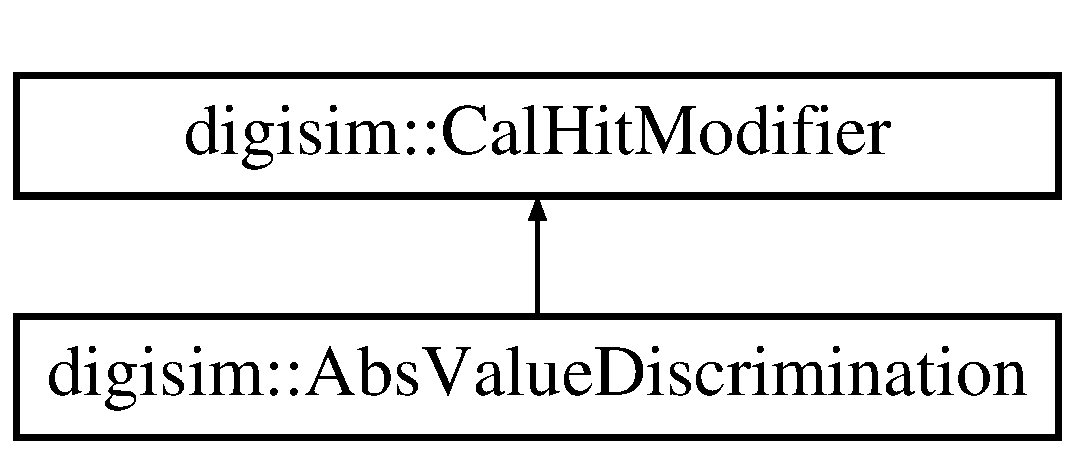
\includegraphics[height=2.000000cm]{classdigisim_1_1AbsValueDiscrimination}
\end{center}
\end{figure}
\subsection*{Public Member Functions}
\begin{DoxyCompactItemize}
\item 
{\bf Abs\-Value\-Discrimination} $\ast$ {\bf new\-Instance} (const std\-::string \&mod\-Name)\label{classdigisim_1_1AbsValueDiscrimination_a1db92197f198684ebaace4c44eba3fc1}

\begin{DoxyCompactList}\small\item\em Returns a reference to a new instance. \end{DoxyCompactList}\item 
{\bf Abs\-Value\-Discrimination} ()\label{classdigisim_1_1AbsValueDiscrimination_ad39b38c00ab0eeb46c6ec2725f8efc26}

\begin{DoxyCompactList}\small\item\em default constructor is only called for global instance \end{DoxyCompactList}\item 
void {\bf init} (std\-::vector$<$ float $>$ \&floats)\label{classdigisim_1_1AbsValueDiscrimination_abb76d9c9d5cfca1b97c03c88546e2ff3}

\begin{DoxyCompactList}\small\item\em initialize parameters \end{DoxyCompactList}\item 
void {\bfseries process\-Hits} (std\-::map$<$ long long, {\bf Temp\-Cal\-Hit} $>$ \&hitmap)\label{classdigisim_1_1AbsValueDiscrimination_a496dc708cd67c488028a4dd32184d08a}

\item 
void {\bf print} () const \label{classdigisim_1_1AbsValueDiscrimination_a935f03f2376371399435dadaf72bb3a4}

\begin{DoxyCompactList}\small\item\em debugging printout \end{DoxyCompactList}\end{DoxyCompactItemize}
\subsection*{Private Member Functions}
\begin{DoxyCompactItemize}
\item 
{\bfseries Abs\-Value\-Discrimination} (const std\-::string \&mod\-Name)\label{classdigisim_1_1AbsValueDiscrimination_af39b9771f74291127789faef98433b6b}

\item 
{\bfseries Abs\-Value\-Discrimination} (const {\bf Abs\-Value\-Discrimination} \&rhs)\label{classdigisim_1_1AbsValueDiscrimination_a0baeb9c354ae71e6b9c06c1f9ceec615}

\item 
bool {\bf is\-Between\-Thresholds} (double energy)\label{classdigisim_1_1AbsValueDiscrimination_adb4b98caa13a3f8f1f93552740684216}

\begin{DoxyCompactList}\small\item\em transformation functions\-: discrimination \end{DoxyCompactList}\end{DoxyCompactItemize}
\subsection*{Private Attributes}
\begin{DoxyCompactItemize}
\item 
std\-::vector$<$ float $>$ {\bf \-\_\-par}\label{classdigisim_1_1AbsValueDiscrimination_a81d100079e51de374bfbc82fcdcecefc}

\begin{DoxyCompactList}\small\item\em Parameters\-: gain and threshold. \end{DoxyCompactList}\end{DoxyCompactItemize}
\subsection*{Additional Inherited Members}


\subsection{Detailed Description}


Definition at line 11 of file Abs\-Value\-Discrimination.\-hpp.



The documentation for this class was generated from the following files\-:\begin{DoxyCompactItemize}
\item 
Abs\-Value\-Discrimination.\-hpp\item 
Abs\-Value\-Discrimination.\-cpp\end{DoxyCompactItemize}

\section{C\-A\-L\-I\-C\-E\-:\-:Ahc2\-Append\-Processor Class Reference}
\label{classCALICE_1_1Ahc2AppendProcessor}\index{C\-A\-L\-I\-C\-E\-::\-Ahc2\-Append\-Processor@{C\-A\-L\-I\-C\-E\-::\-Ahc2\-Append\-Processor}}


Processor which allows to append events from additional L\-C\-I\-O files.  




{\ttfamily \#include $<$Ahc2\-Append\-Processor.\-hh$>$}

Inheritance diagram for C\-A\-L\-I\-C\-E\-:\-:Ahc2\-Append\-Processor\-:\begin{figure}[H]
\begin{center}
\leavevmode
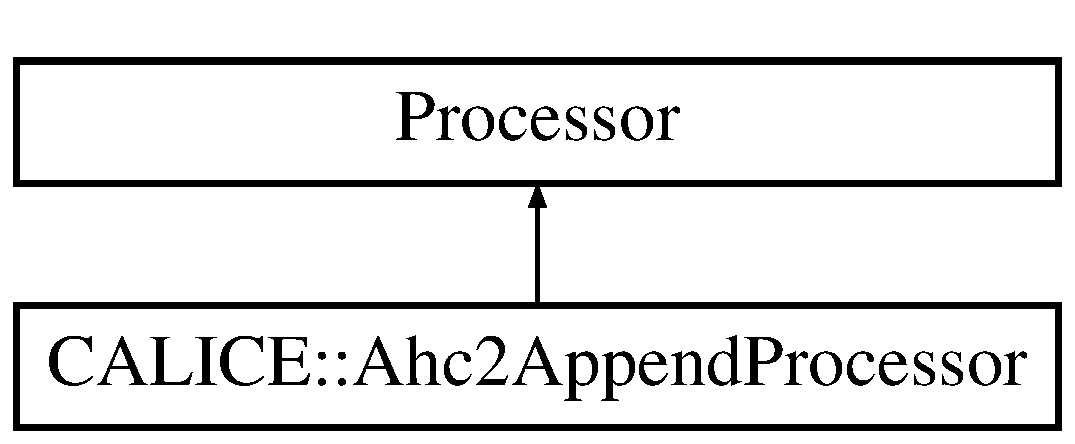
\includegraphics[height=2.000000cm]{classCALICE_1_1Ahc2AppendProcessor}
\end{center}
\end{figure}
\subsection*{Public Member Functions}
\begin{DoxyCompactItemize}
\item 
virtual Processor $\ast$ {\bfseries new\-Processor} ()\label{classCALICE_1_1Ahc2AppendProcessor_a5008f6b9bfc17a27630f14764a2746d2}

\item 
{\bf Ahc2\-Append\-Processor} ()\label{classCALICE_1_1Ahc2AppendProcessor_ae2d1110a71e12f08ba04ddd44db765de}

\begin{DoxyCompactList}\small\item\em Constructor. \end{DoxyCompactList}\item 
{\bf $\sim$\-Ahc2\-Append\-Processor} ()\label{classCALICE_1_1Ahc2AppendProcessor_ae2e9652363dfc5fcf5c95e34e731e7b5}

\begin{DoxyCompactList}\small\item\em Destructor. \end{DoxyCompactList}\item 
virtual void {\bf init} ()\label{classCALICE_1_1Ahc2AppendProcessor_a1bd0b7774d169ebcc9f5387df38d09c2}

\begin{DoxyCompactList}\small\item\em Initialise. \end{DoxyCompactList}\item 
virtual void {\bf process\-Event} (lcio\-::\-L\-C\-Event $\ast$evt)\label{classCALICE_1_1Ahc2AppendProcessor_ac818e075407b86aff4d03fb9a4edfe6e}

\begin{DoxyCompactList}\small\item\em Process event (the working horse) \end{DoxyCompactList}\end{DoxyCompactItemize}
\subsection*{Protected Attributes}
\begin{DoxyCompactItemize}
\item 
lcio\-::\-String\-Vec {\bf \-\_\-append\-File\-Names}\label{classCALICE_1_1Ahc2AppendProcessor_a20d46a95a43820da5b94ef213d78740c}

\begin{DoxyCompactList}\small\item\em vector of names of input files \end{DoxyCompactList}\item 
lcio\-::\-String\-Vec {\bf \-\_\-append\-Collection\-Input\-Names}\label{classCALICE_1_1Ahc2AppendProcessor_a630978ff6d3a72e76b38cda94d5ac7b2}

\begin{DoxyCompactList}\small\item\em name of the input collection to append \end{DoxyCompactList}\item 
lcio\-::\-String\-Vec {\bf \-\_\-append\-Collection\-Output\-Names}\label{classCALICE_1_1Ahc2AppendProcessor_acaef8b9543548dd47d24dff92b39d517}

\begin{DoxyCompactList}\small\item\em name of the output collection after appending \end{DoxyCompactList}\item 
lcio\-::\-L\-C\-Reader $\ast$ {\bf \-\_\-lc\-Reader}\label{classCALICE_1_1Ahc2AppendProcessor_a5339bbd6d833f8ba7d24ce45304965b0}

\begin{DoxyCompactList}\small\item\em Reader in L\-C\-I\-O to open a file. \end{DoxyCompactList}\item 
bool {\bf \-\_\-append\-Repeat\-Collections}\label{classCALICE_1_1Ahc2AppendProcessor_af4ac88f656de0d4b35f96c360e3d4a25}

\begin{DoxyCompactList}\small\item\em continue appending after end of appending file (loop again over events) \end{DoxyCompactList}\end{DoxyCompactItemize}


\subsection{Detailed Description}
Processor which allows to append events from additional L\-C\-I\-O files. 

\begin{DoxyAuthor}{Author}
{\tt eldwan.\-brianne@desy.\-de} 
\end{DoxyAuthor}
\begin{DoxyVersion}{Version}
1.\-0 
\end{DoxyVersion}
\begin{DoxyDate}{Date}
Decmeber 2015 
\end{DoxyDate}


Definition at line 17 of file Ahc2\-Append\-Processor.\-hh.



The documentation for this class was generated from the following files\-:\begin{DoxyCompactItemize}
\item 
Ahc2\-Append\-Processor.\-hh\item 
Ahc2\-Append\-Processor.\-cc\end{DoxyCompactItemize}

\section{C\-A\-L\-I\-C\-E\-:\-:Ahc2\-Collection\-Merger Class Reference}
\label{classCALICE_1_1Ahc2CollectionMerger}\index{C\-A\-L\-I\-C\-E\-::\-Ahc2\-Collection\-Merger@{C\-A\-L\-I\-C\-E\-::\-Ahc2\-Collection\-Merger}}


Processor which allows to merge collections from the same event (use for D\-D4\-H\-E\-P).  




{\ttfamily \#include $<$Ahc2\-Collection\-Merger.\-hh$>$}

Inheritance diagram for C\-A\-L\-I\-C\-E\-:\-:Ahc2\-Collection\-Merger\-:\begin{figure}[H]
\begin{center}
\leavevmode
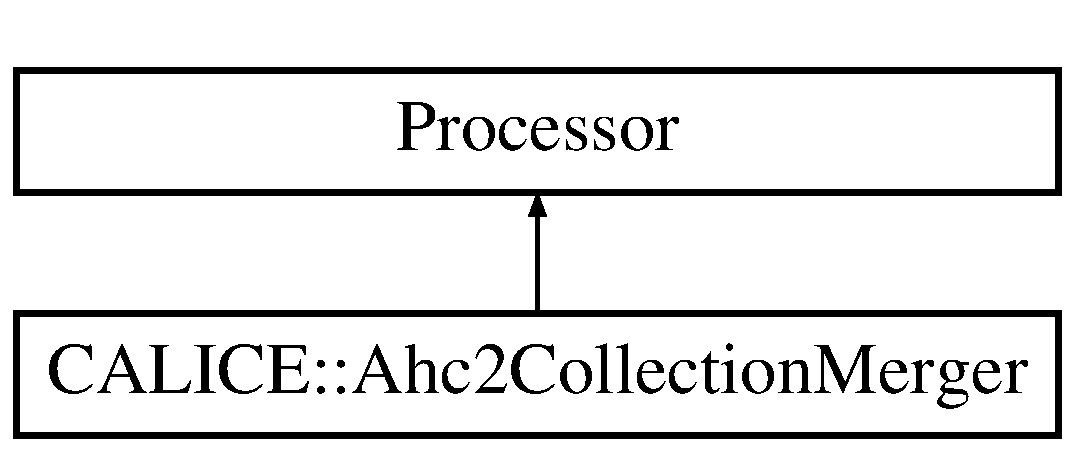
\includegraphics[height=2.000000cm]{classCALICE_1_1Ahc2CollectionMerger}
\end{center}
\end{figure}
\subsection*{Public Member Functions}
\begin{DoxyCompactItemize}
\item 
virtual Processor $\ast$ {\bfseries new\-Processor} ()\label{classCALICE_1_1Ahc2CollectionMerger_aadaac89942c47bef56cb419e5b54faf2}

\item 
{\bf Ahc2\-Collection\-Merger} ()\label{classCALICE_1_1Ahc2CollectionMerger_ac9e200f03523dd0822b91ca9b1d3843b}

\begin{DoxyCompactList}\small\item\em Constructor. \end{DoxyCompactList}\item 
{\bf $\sim$\-Ahc2\-Collection\-Merger} ()\label{classCALICE_1_1Ahc2CollectionMerger_a632fafa0ad0ee8b40f144117e4cc4ab9}

\begin{DoxyCompactList}\small\item\em Destructor. \end{DoxyCompactList}\item 
virtual void {\bf init} ()\label{classCALICE_1_1Ahc2CollectionMerger_a60857818e89b706e239a68e839188384}

\begin{DoxyCompactList}\small\item\em Initialise. \end{DoxyCompactList}\item 
virtual void {\bf process\-Event} (lcio\-::\-L\-C\-Event $\ast$evt)\label{classCALICE_1_1Ahc2CollectionMerger_a825abffb2abb11a2cade1ecb0056ee09}

\begin{DoxyCompactList}\small\item\em Process event (the working horse) \end{DoxyCompactList}\end{DoxyCompactItemize}
\subsection*{Protected Attributes}
\begin{DoxyCompactItemize}
\item 
lcio\-::\-String\-Vec {\bf \-\_\-\-Collection\-Input\-Names}\label{classCALICE_1_1Ahc2CollectionMerger_aa915f7a73842f950b1024bd4febf15fc}

\begin{DoxyCompactList}\small\item\em name of the input collection to append \end{DoxyCompactList}\item 
std\-::string {\bf \-\_\-\-Collection\-Output\-Name}\label{classCALICE_1_1Ahc2CollectionMerger_a1078419aa8e347575549cf1036ae58b7}

\begin{DoxyCompactList}\small\item\em name of the output collection after appending \end{DoxyCompactList}\item 
std\-::string {\bfseries \-\_\-encoding}\label{classCALICE_1_1Ahc2CollectionMerger_a92ea968b43e51fe59f49da396bfa62e2}

\end{DoxyCompactItemize}


\subsection{Detailed Description}
Processor which allows to merge collections from the same event (use for D\-D4\-H\-E\-P). 

\begin{DoxyAuthor}{Author}
{\tt eldwan.\-brianne@desy.\-de} 
\end{DoxyAuthor}
\begin{DoxyVersion}{Version}
1.\-0 
\end{DoxyVersion}
\begin{DoxyDate}{Date}
September 2016 
\end{DoxyDate}


Definition at line 17 of file Ahc2\-Collection\-Merger.\-hh.



The documentation for this class was generated from the following files\-:\begin{DoxyCompactItemize}
\item 
Ahc2\-Collection\-Merger.\-hh\item 
Ahc2\-Collection\-Merger.\-cc\end{DoxyCompactItemize}

\section{C\-A\-L\-I\-C\-E\-:\-:Ahc2\-Ganging\-Processor Class Reference}
\label{classCALICE_1_1Ahc2GangingProcessor}\index{C\-A\-L\-I\-C\-E\-::\-Ahc2\-Ganging\-Processor@{C\-A\-L\-I\-C\-E\-::\-Ahc2\-Ganging\-Processor}}


The processor performing the ganging.  




{\ttfamily \#include $<$Ahc2\-Ganging\-Processor.\-hh$>$}

Inheritance diagram for C\-A\-L\-I\-C\-E\-:\-:Ahc2\-Ganging\-Processor\-:\begin{figure}[H]
\begin{center}
\leavevmode
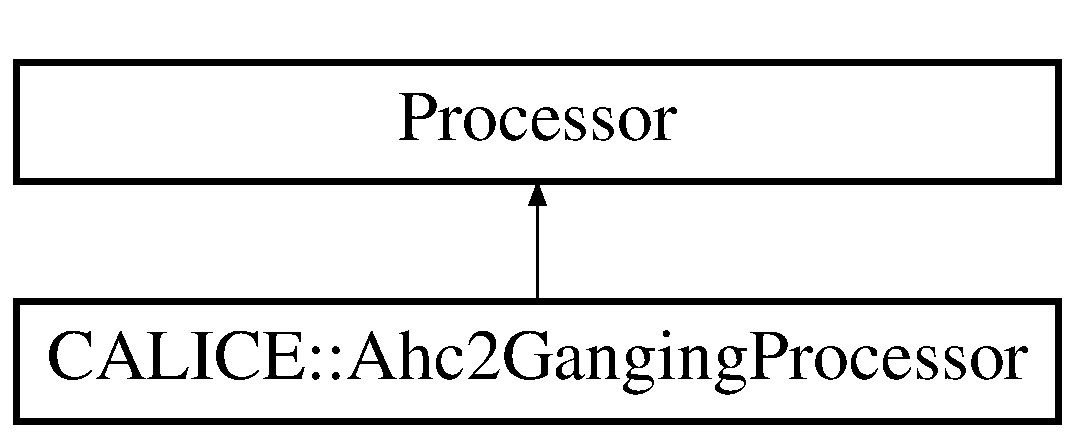
\includegraphics[height=2.000000cm]{classCALICE_1_1Ahc2GangingProcessor}
\end{center}
\end{figure}
\subsection*{Public Member Functions}
\begin{DoxyCompactItemize}
\item 
virtual Processor $\ast$ {\bfseries new\-Processor} ()\label{classCALICE_1_1Ahc2GangingProcessor_a641c4981d0a6e6b7262c533afef6610d}

\item 
virtual void {\bf init} ()
\begin{DoxyCompactList}\small\item\em Initiliases the ganging chain of responsibilty for fine and coarse modules. \end{DoxyCompactList}\item 
virtual void {\bf process\-Event} (lcio\-::\-L\-C\-Event $\ast$evt)\label{classCALICE_1_1Ahc2GangingProcessor_aabe6735d2ee4a77ea0b0f4471f3084f0}

\begin{DoxyCompactList}\small\item\em Called every event. \end{DoxyCompactList}\item 
float {\bf energy\-Sum} (std\-::vector$<$ Sim\-Calorimeter\-Hit $\ast$ $>$ vec\-Sim\-Hits)\label{classCALICE_1_1Ahc2GangingProcessor_a559c0975eaf8a4ba34865b0c61f9f44e}

\begin{DoxyCompactList}\small\item\em Helper function to add up all Sim\-Calorimeter\-Hit energies. \end{DoxyCompactList}\item 
virtual void {\bf create\-Output\-Collections} (lcio\-::\-L\-C\-Event $\ast$evt)\label{classCALICE_1_1Ahc2GangingProcessor_ac0ec34c59d8e08ef566d90bd3db0806d}

\begin{DoxyCompactList}\small\item\em Creates the ganged collection. \end{DoxyCompactList}\item 
virtual void {\bf tidy\-Up} ()\label{classCALICE_1_1Ahc2GangingProcessor_a77c89cea49112c5ae23a0f7cfa547514}

\begin{DoxyCompactList}\small\item\em Resets everything which is event specific. \end{DoxyCompactList}\item 
virtual void {\bfseries print\-Parameters} ()\label{classCALICE_1_1Ahc2GangingProcessor_aa992fa2e0139efbac4ca271fddbf4d09}

\item 
void {\bfseries end} ()\label{classCALICE_1_1Ahc2GangingProcessor_a055b34a63fff28f57dbad36e2e019a08}

\end{DoxyCompactItemize}
\subsection*{Protected Attributes}
\begin{DoxyCompactItemize}
\item 
vector$<$ std\-::string $>$ {\bfseries \-\_\-calorim\-Inp\-Collections}\label{classCALICE_1_1Ahc2GangingProcessor_a336a0172cf7433b6c59362856d133139}

\item 
vector$<$ std\-::string $>$ {\bfseries \-\_\-calorim\-Out\-Collections}\label{classCALICE_1_1Ahc2GangingProcessor_a0be4cc687a247ae1cbd8fccb5b9b89c4}

\item 
float {\bfseries \-\_\-tile\-Border\-Attenuation\-Factor}\label{classCALICE_1_1Ahc2GangingProcessor_a60ca794d80683e32799d3e15db651f40}

\item 
int {\bfseries \-\_\-\-Tokyo\-Layer}\label{classCALICE_1_1Ahc2GangingProcessor_ab7f3b82677dc2fa66ef598f26efc787a}

\item 
{\bf Contribution\-Map} {\bf \-\_\-contribution\-Map}
\begin{DoxyCompactList}\small\item\em Instance which holds the gather Sim\-Calorimeter\-Hits. \end{DoxyCompactList}\item 
std\-::vector$<$ {\bf Ganger} $\ast$ $>$ {\bf \-\_\-gangers\-For\-Tokyo\-Module}
\begin{DoxyCompactList}\small\item\em All gangers needed for a tokyo module. \end{DoxyCompactList}\end{DoxyCompactItemize}


\subsection{Detailed Description}
The processor performing the ganging. 

Definition at line 59 of file Ahc2\-Ganging\-Processor.\-hh.



\subsection{Member Function Documentation}
\index{C\-A\-L\-I\-C\-E\-::\-Ahc2\-Ganging\-Processor@{C\-A\-L\-I\-C\-E\-::\-Ahc2\-Ganging\-Processor}!init@{init}}
\index{init@{init}!CALICE::Ahc2GangingProcessor@{C\-A\-L\-I\-C\-E\-::\-Ahc2\-Ganging\-Processor}}
\subsubsection[{init}]{\setlength{\rightskip}{0pt plus 5cm}void C\-A\-L\-I\-C\-E\-::\-Ahc2\-Ganging\-Processor\-::init (
\begin{DoxyParamCaption}
{}
\end{DoxyParamCaption}
)\hspace{0.3cm}{\ttfamily [virtual]}}\label{classCALICE_1_1Ahc2GangingProcessor_a85e1628f6cc79278e8fa51be8e41bcf6}


Initiliases the ganging chain of responsibilty for fine and coarse modules. 

Defines location of module types. 

Definition at line 76 of file Ahc2\-Ganging\-Processor.\-cc.



References \-\_\-contribution\-Map, and \-\_\-gangers\-For\-Tokyo\-Module.



\subsection{Field Documentation}
\index{C\-A\-L\-I\-C\-E\-::\-Ahc2\-Ganging\-Processor@{C\-A\-L\-I\-C\-E\-::\-Ahc2\-Ganging\-Processor}!\-\_\-contribution\-Map@{\-\_\-contribution\-Map}}
\index{\-\_\-contribution\-Map@{\-\_\-contribution\-Map}!CALICE::Ahc2GangingProcessor@{C\-A\-L\-I\-C\-E\-::\-Ahc2\-Ganging\-Processor}}
\subsubsection[{\-\_\-contribution\-Map}]{\setlength{\rightskip}{0pt plus 5cm}{\bf Contribution\-Map} C\-A\-L\-I\-C\-E\-::\-Ahc2\-Ganging\-Processor\-::\-\_\-contribution\-Map\hspace{0.3cm}{\ttfamily [protected]}}\label{classCALICE_1_1Ahc2GangingProcessor_af9493a3b058b1da01eb61a750fa00dde}


Instance which holds the gather Sim\-Calorimeter\-Hits. 

The outcome of the ganging is here. 

Definition at line 109 of file Ahc2\-Ganging\-Processor.\-hh.



Referenced by create\-Output\-Collections(), init(), and tidy\-Up().

\index{C\-A\-L\-I\-C\-E\-::\-Ahc2\-Ganging\-Processor@{C\-A\-L\-I\-C\-E\-::\-Ahc2\-Ganging\-Processor}!\-\_\-gangers\-For\-Tokyo\-Module@{\-\_\-gangers\-For\-Tokyo\-Module}}
\index{\-\_\-gangers\-For\-Tokyo\-Module@{\-\_\-gangers\-For\-Tokyo\-Module}!CALICE::Ahc2GangingProcessor@{C\-A\-L\-I\-C\-E\-::\-Ahc2\-Ganging\-Processor}}
\subsubsection[{\-\_\-gangers\-For\-Tokyo\-Module}]{\setlength{\rightskip}{0pt plus 5cm}std\-::vector$<${\bf Ganger}$\ast$$>$ C\-A\-L\-I\-C\-E\-::\-Ahc2\-Ganging\-Processor\-::\-\_\-gangers\-For\-Tokyo\-Module\hspace{0.3cm}{\ttfamily [protected]}}\label{classCALICE_1_1Ahc2GangingProcessor_abbfd0274ca1053690374699f6dd8ae2d}


All gangers needed for a tokyo module. 

Filled in \doxyref{init()}{p.}{classCALICE_1_1Ahc2GangingProcessor_a85e1628f6cc79278e8fa51be8e41bcf6}. 

Definition at line 113 of file Ahc2\-Ganging\-Processor.\-hh.



Referenced by init(), and process\-Event().



The documentation for this class was generated from the following files\-:\begin{DoxyCompactItemize}
\item 
Ahc2\-Ganging\-Processor.\-hh\item 
Ahc2\-Ganging\-Processor.\-cc\end{DoxyCompactItemize}

\section{C\-A\-L\-I\-C\-E\-:\-:Ahc2\-M\-I\-P2\-Ge\-V\-Processor Class Reference}
\label{classCALICE_1_1Ahc2MIP2GeVProcessor}\index{C\-A\-L\-I\-C\-E\-::\-Ahc2\-M\-I\-P2\-Ge\-V\-Processor@{C\-A\-L\-I\-C\-E\-::\-Ahc2\-M\-I\-P2\-Ge\-V\-Processor}}


Class doing the conversion between Ge\-V and M\-I\-P + Correction of K layer (not smart!!)  




{\ttfamily \#include $<$Ahc2\-M\-I\-P2\-Ge\-V\-Processor.\-hh$>$}

Inheritance diagram for C\-A\-L\-I\-C\-E\-:\-:Ahc2\-M\-I\-P2\-Ge\-V\-Processor\-:\begin{figure}[H]
\begin{center}
\leavevmode
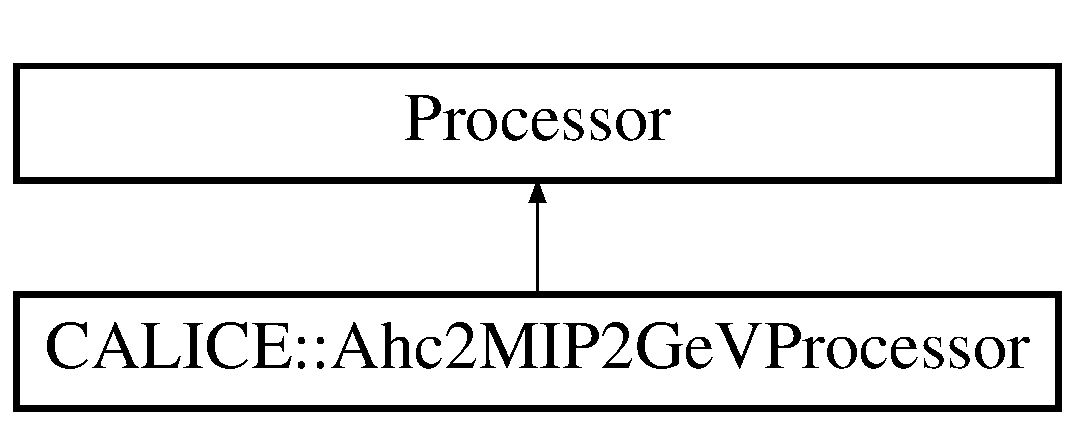
\includegraphics[height=2.000000cm]{classCALICE_1_1Ahc2MIP2GeVProcessor}
\end{center}
\end{figure}
\subsection*{Public Member Functions}
\begin{DoxyCompactItemize}
\item 
virtual Processor $\ast$ {\bfseries new\-Processor} ()\label{classCALICE_1_1Ahc2MIP2GeVProcessor_a7298172c4de82d57129cd2e5ae36f68b}

\item 
{\bf Ahc2\-M\-I\-P2\-Ge\-V\-Processor} ()\label{classCALICE_1_1Ahc2MIP2GeVProcessor_ab777ee23a63f9b782a8b62713c586835}

\begin{DoxyCompactList}\small\item\em Constructor. \end{DoxyCompactList}\item 
{\bf $\sim$\-Ahc2\-M\-I\-P2\-Ge\-V\-Processor} ()\label{classCALICE_1_1Ahc2MIP2GeVProcessor_ac4250234a03cfe94edd099dcada58d43}

\begin{DoxyCompactList}\small\item\em Destructor. \end{DoxyCompactList}\item 
virtual void {\bf init} ()\label{classCALICE_1_1Ahc2MIP2GeVProcessor_aeaaccd22b995e22688ec235d19230427}

\begin{DoxyCompactList}\small\item\em Initialise. \end{DoxyCompactList}\item 
virtual void {\bf process\-Run\-Header} (L\-C\-Run\-Header $\ast$run)\label{classCALICE_1_1Ahc2MIP2GeVProcessor_af3e43eb5e4f6ba85f86bea5d43985485}

\begin{DoxyCompactList}\small\item\em Process header. \end{DoxyCompactList}\item 
virtual void {\bf process\-Event} (L\-C\-Event $\ast$evt)\label{classCALICE_1_1Ahc2MIP2GeVProcessor_ac8478160bdb78253c8fe0f6a37049ef5}

\begin{DoxyCompactList}\small\item\em Process event (the working horse) \end{DoxyCompactList}\item 
virtual void {\bf check} (L\-C\-Event $\ast$evt)\label{classCALICE_1_1Ahc2MIP2GeVProcessor_ab7bc36ceb4918f6e9887056335c32587}

\begin{DoxyCompactList}\small\item\em Check. \end{DoxyCompactList}\item 
virtual void {\bf end} ()\label{classCALICE_1_1Ahc2MIP2GeVProcessor_ae0c106a5baa6cffe68639653bf079a67}

\begin{DoxyCompactList}\small\item\em End of processing. \end{DoxyCompactList}\item 
virtual void {\bf print\-Parameters} ()\label{classCALICE_1_1Ahc2MIP2GeVProcessor_ae502a5cb0cc0eaeaa63440ccbd7654cf}

\begin{DoxyCompactList}\small\item\em Print Parameters. \end{DoxyCompactList}\item 
virtual void {\bf Fill\-Map\-K} ()\label{classCALICE_1_1Ahc2MIP2GeVProcessor_a7e200e2780196bdac74de34c48b0e8ea}

\begin{DoxyCompactList}\small\item\em Fill the K map. \end{DoxyCompactList}\end{DoxyCompactItemize}
\subsection*{Protected Attributes}
\begin{DoxyCompactItemize}
\item 
std\-::string {\bf \-\_\-calorim\-Inp\-Collection}\label{classCALICE_1_1Ahc2MIP2GeVProcessor_ac98bb5f559ade9930981b45e6af647df}

\begin{DoxyCompactList}\small\item\em input collection name \end{DoxyCompactList}\item 
std\-::string {\bf \-\_\-calorim\-Out\-Collection}\label{classCALICE_1_1Ahc2MIP2GeVProcessor_abc3aa68a225b5247bcf939ac444e8e3c}

\begin{DoxyCompactList}\small\item\em output collection name \end{DoxyCompactList}\item 
vector$<$ std\-::string $>$ {\bf \-\_\-calorim\-Inp\-Collections}\label{classCALICE_1_1Ahc2MIP2GeVProcessor_a1cbcfad20f4a1442e348069c0ee3ce4a}

\begin{DoxyCompactList}\small\item\em input collection name \end{DoxyCompactList}\item 
vector$<$ std\-::string $>$ {\bf \-\_\-calorim\-Out\-Collections}\label{classCALICE_1_1Ahc2MIP2GeVProcessor_aeac8962705d46a9508e48c5d09a11e80}

\begin{DoxyCompactList}\small\item\em output collection name \end{DoxyCompactList}\item 
std\-::string {\bfseries \-\_\-encoding}\label{classCALICE_1_1Ahc2MIP2GeVProcessor_adab396f0c5d55740e531225e7e4ce65d}

\item 
std\-::string {\bfseries \-\_\-file\-Map\-K}\label{classCALICE_1_1Ahc2MIP2GeVProcessor_af0b9513edea9da93c8a3a3c52f2e39b4}

\item 
std\-::map$<$ int, std\-::map$<$ int, \\*
int $>$ $>$ {\bf \-\_\-map\-K}
\begin{DoxyCompactList}\small\item\em File containing the relation between K in Simulation and K in data. \end{DoxyCompactList}\item 
int {\bf \-\_\-n\-Run}\label{classCALICE_1_1Ahc2MIP2GeVProcessor_af41b36a5429f50a0eab3ac38a5f66c7f}

\begin{DoxyCompactList}\small\item\em run number \end{DoxyCompactList}\item 
int {\bf \-\_\-n\-Evt}\label{classCALICE_1_1Ahc2MIP2GeVProcessor_a9cdc466f2b1bd0bbb10dc7e485652369}

\begin{DoxyCompactList}\small\item\em evt number \end{DoxyCompactList}\end{DoxyCompactItemize}
\subsection*{Private Attributes}
\begin{DoxyCompactItemize}
\item 
float {\bf \-\_\-\-M\-I\-Pvalue}\label{classCALICE_1_1Ahc2MIP2GeVProcessor_a30a2596fee76d2e4f13197348c432937}

\begin{DoxyCompactList}\small\item\em M\-I\-P conversion factor in Ge\-V. \end{DoxyCompactList}\item 
std\-::string {\bf \-\_\-rootfilename}\label{classCALICE_1_1Ahc2MIP2GeVProcessor_a7c0a3d4389476c59205c221b662762e6}

\begin{DoxyCompactList}\small\item\em rootfile name \end{DoxyCompactList}\end{DoxyCompactItemize}


\subsection{Detailed Description}
Class doing the conversion between Ge\-V and M\-I\-P + Correction of K layer (not smart!!) 

\begin{DoxyAuthor}{Author}
{\tt eldwan.\-brianne@desy.\-de} 
\end{DoxyAuthor}
\begin{DoxyVersion}{Version}
1.\-0 
\end{DoxyVersion}
\begin{DoxyDate}{Date}
November 2015 
\end{DoxyDate}


Definition at line 30 of file Ahc2\-M\-I\-P2\-Ge\-V\-Processor.\-hh.



\subsection{Field Documentation}
\index{C\-A\-L\-I\-C\-E\-::\-Ahc2\-M\-I\-P2\-Ge\-V\-Processor@{C\-A\-L\-I\-C\-E\-::\-Ahc2\-M\-I\-P2\-Ge\-V\-Processor}!\-\_\-map\-K@{\-\_\-map\-K}}
\index{\-\_\-map\-K@{\-\_\-map\-K}!CALICE::Ahc2MIP2GeVProcessor@{C\-A\-L\-I\-C\-E\-::\-Ahc2\-M\-I\-P2\-Ge\-V\-Processor}}
\subsubsection[{\-\_\-map\-K}]{\setlength{\rightskip}{0pt plus 5cm}std\-::map$<$int,std\-::map$<$int,int$>$ $>$ C\-A\-L\-I\-C\-E\-::\-Ahc2\-M\-I\-P2\-Ge\-V\-Processor\-::\-\_\-map\-K\hspace{0.3cm}{\ttfamily [protected]}}\label{classCALICE_1_1Ahc2MIP2GeVProcessor_a796ade5fb97078104c67acf0b6a6b77e}


File containing the relation between K in Simulation and K in data. 

map containing Sim\-K and K to convert 

Definition at line 89 of file Ahc2\-M\-I\-P2\-Ge\-V\-Processor.\-hh.



Referenced by Fill\-Map\-K(), init(), and process\-Event().



The documentation for this class was generated from the following files\-:\begin{DoxyCompactItemize}
\item 
Ahc2\-M\-I\-P2\-Ge\-V\-Processor.\-hh\item 
Ahc2\-M\-I\-P2\-Ge\-V\-Processor.\-cc\end{DoxyCompactItemize}

\section{C\-A\-L\-I\-C\-E\-:\-:Ahc2\-R\-O\-C\-Threshold\-Processor Class Reference}
\label{classCALICE_1_1Ahc2ROCThresholdProcessor}\index{C\-A\-L\-I\-C\-E\-::\-Ahc2\-R\-O\-C\-Threshold\-Processor@{C\-A\-L\-I\-C\-E\-::\-Ahc2\-R\-O\-C\-Threshold\-Processor}}


Class for doing the \doxyref{A\-H\-C\-A\-L}{p.}{namespaceCALICE_1_1AHCAL} R\-O\-C Simulating behavior.  




{\ttfamily \#include $<$Ahc2\-R\-O\-C\-Threshold\-Processor.\-hh$>$}

Inheritance diagram for C\-A\-L\-I\-C\-E\-:\-:Ahc2\-R\-O\-C\-Threshold\-Processor\-:\begin{figure}[H]
\begin{center}
\leavevmode
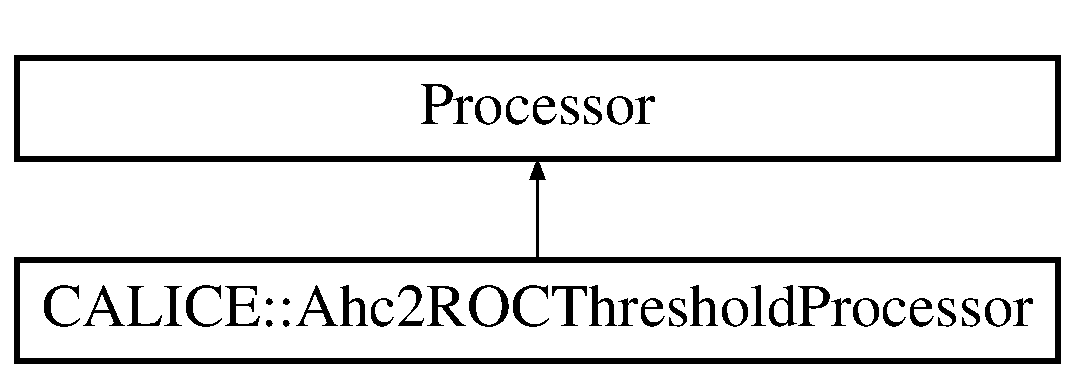
\includegraphics[height=2.000000cm]{classCALICE_1_1Ahc2ROCThresholdProcessor}
\end{center}
\end{figure}
\subsection*{Public Member Functions}
\begin{DoxyCompactItemize}
\item 
virtual Processor $\ast$ {\bfseries new\-Processor} ()\label{classCALICE_1_1Ahc2ROCThresholdProcessor_aa193ba020919b40c3c91085a1cc66d4a}

\item 
{\bf Ahc2\-R\-O\-C\-Threshold\-Processor} ()\label{classCALICE_1_1Ahc2ROCThresholdProcessor_ab1704441505945a9dcbc47b80f16566e}

\begin{DoxyCompactList}\small\item\em Constructor. \end{DoxyCompactList}\item 
{\bf $\sim$\-Ahc2\-R\-O\-C\-Threshold\-Processor} ()\label{classCALICE_1_1Ahc2ROCThresholdProcessor_ab6ff1870b195412741211db8610501bb}

\begin{DoxyCompactList}\small\item\em Destructor. \end{DoxyCompactList}\item 
virtual void {\bf init} ()\label{classCALICE_1_1Ahc2ROCThresholdProcessor_a9cccdbb4240bba916ff6dc81f5a2d7cf}

\begin{DoxyCompactList}\small\item\em Initialise. \end{DoxyCompactList}\item 
virtual void {\bf process\-Run\-Header} (L\-C\-Run\-Header $\ast$run)\label{classCALICE_1_1Ahc2ROCThresholdProcessor_a2e3340c95492818108566bd06a667c66}

\begin{DoxyCompactList}\small\item\em Process header. \end{DoxyCompactList}\item 
virtual void {\bf process\-Event} (L\-C\-Event $\ast$evt)\label{classCALICE_1_1Ahc2ROCThresholdProcessor_a7ecbc0929e784e429d53914b26a4d9b9}

\begin{DoxyCompactList}\small\item\em Process event (the working horse) \end{DoxyCompactList}\item 
virtual void {\bf check} (L\-C\-Event $\ast$evt)\label{classCALICE_1_1Ahc2ROCThresholdProcessor_ab026a8529bb96eb43757f708c4e63356}

\begin{DoxyCompactList}\small\item\em Check. \end{DoxyCompactList}\item 
virtual void {\bf end} ()\label{classCALICE_1_1Ahc2ROCThresholdProcessor_ae39dacafb2a8b2e07a087b4cae04a7a0}

\begin{DoxyCompactList}\small\item\em End of processing. \end{DoxyCompactList}\item 
virtual void {\bf print\-Parameters} ()\label{classCALICE_1_1Ahc2ROCThresholdProcessor_ae6d62f6232c14fb7038fe08701e57be2}

\begin{DoxyCompactList}\small\item\em Print Parameters. \end{DoxyCompactList}\end{DoxyCompactItemize}
\subsection*{Protected Attributes}
\begin{DoxyCompactItemize}
\item 
std\-::string {\bf \-\_\-calorim\-Inp\-Collection}\label{classCALICE_1_1Ahc2ROCThresholdProcessor_a60b33e4ec2f8859870691b0a5a9b06c4}

\begin{DoxyCompactList}\small\item\em input collection name \end{DoxyCompactList}\item 
std\-::string {\bf \-\_\-calorim\-Out\-Collection}\label{classCALICE_1_1Ahc2ROCThresholdProcessor_a5bbe60c8516f421ff31879e318b77c9d}

\begin{DoxyCompactList}\small\item\em output collection name \end{DoxyCompactList}\item 
vector$<$ std\-::string $>$ {\bf \-\_\-calorim\-Inp\-Collections}\label{classCALICE_1_1Ahc2ROCThresholdProcessor_a84c9fa484bf114809c283bcd098cb7c5}

\begin{DoxyCompactList}\small\item\em input collection name \end{DoxyCompactList}\item 
vector$<$ std\-::string $>$ {\bf \-\_\-calorim\-Out\-Collections}\label{classCALICE_1_1Ahc2ROCThresholdProcessor_ae774780c23556903916980a556048672}

\begin{DoxyCompactList}\small\item\em output collection name \end{DoxyCompactList}\item 
std\-::string {\bfseries \-\_\-encoding}\label{classCALICE_1_1Ahc2ROCThresholdProcessor_ae52fc82c424c5b0692e68b8ce7fc4a46}

\item 
float {\bf energy\-Threshold}\label{classCALICE_1_1Ahc2ROCThresholdProcessor_ae03d5ba16a2f892a15cff2ca19b03475}

\begin{DoxyCompactList}\small\item\em Threshold. \end{DoxyCompactList}\item 
float {\bf halfd\-S}\label{classCALICE_1_1Ahc2ROCThresholdProcessor_a19a4d90c4ac1a4c1ec6d5c68ffa53b1d}

\begin{DoxyCompactList}\small\item\em half dead space \end{DoxyCompactList}\item 
int {\bf \-\_\-n\-Run}\label{classCALICE_1_1Ahc2ROCThresholdProcessor_a96d3965db3c014b35df0e61fa8fafffe}

\begin{DoxyCompactList}\small\item\em run number \end{DoxyCompactList}\item 
int {\bf \-\_\-n\-Evt}\label{classCALICE_1_1Ahc2ROCThresholdProcessor_a10d4875cd898bfa45970886a9bf16bbc}

\begin{DoxyCompactList}\small\item\em event number \end{DoxyCompactList}\item 
std\-::string {\bf \-\_\-mapping\-Processor\-Name}\label{classCALICE_1_1Ahc2ROCThresholdProcessor_a31029f43ae89b71d54cc88c6a4c3eb40}

\begin{DoxyCompactList}\small\item\em name of the processor which provides the mapping \end{DoxyCompactList}\item 
std\-::string {\bf \-\_\-calib\-Processor\-Name}\label{classCALICE_1_1Ahc2ROCThresholdProcessor_a314178c8fbcc0a6bb9765ff801b9c903}

\begin{DoxyCompactList}\small\item\em name of the processor which provides the Si\-P\-M calibrations \end{DoxyCompactList}\item 
const Ahc2\-Mapper $\ast$ {\bf \-\_\-mapper}\label{classCALICE_1_1Ahc2ROCThresholdProcessor_a6d60f00fdd551a8102f1a5232669f4b6}

\begin{DoxyCompactList}\small\item\em the mapper \end{DoxyCompactList}\item 
Mapped\-Container\\*
$<$ Ahc2\-Calibrations $>$ $\ast$ {\bf \-\_\-calib\-Container}\label{classCALICE_1_1Ahc2ROCThresholdProcessor_a69041e2f134eee50feaa855f2117104f}

\begin{DoxyCompactList}\small\item\em mapped container of Si\-P\-M calibrations \end{DoxyCompactList}\end{DoxyCompactItemize}
\subsection*{Private Attributes}
\begin{DoxyCompactItemize}
\item 
float {\bf \-\_\-tile\-Edge\-X}\label{classCALICE_1_1Ahc2ROCThresholdProcessor_a016893bc97957f9d94f1e97b4a177518}

\begin{DoxyCompactList}\small\item\em Tile size in X. \end{DoxyCompactList}\item 
float {\bf \-\_\-tile\-Edge\-Y}\label{classCALICE_1_1Ahc2ROCThresholdProcessor_aa18043151bdf9186f48699c9eec0fc1b}

\begin{DoxyCompactList}\small\item\em Tile size in Y. \end{DoxyCompactList}\item 
float {\bf \-\_\-dead\-Space}\label{classCALICE_1_1Ahc2ROCThresholdProcessor_a599dcde5b82f16f8c08badc05c1ee7aa}

\begin{DoxyCompactList}\small\item\em dead space \end{DoxyCompactList}\item 
float {\bf \-\_\-\-M\-I\-Pvalue}\label{classCALICE_1_1Ahc2ROCThresholdProcessor_a5bc9a6cdc1c901f62ec0bd735482cea3}

\begin{DoxyCompactList}\small\item\em M\-I\-P Value. \end{DoxyCompactList}\item 
float {\bf \-\_\-\-M\-I\-P\-Thr}\label{classCALICE_1_1Ahc2ROCThresholdProcessor_a0fd1875b10471d5cd0153fd0a7649473}

\begin{DoxyCompactList}\small\item\em M\-I\-P Threshold. \end{DoxyCompactList}\item 
float {\bf \-\_\-tfast}\label{classCALICE_1_1Ahc2ROCThresholdProcessor_a047fe6811de6d2a4169aed1c703d45c2}

\begin{DoxyCompactList}\small\item\em fast shaper integration time \end{DoxyCompactList}\item 
float {\bf \-\_\-tslow}\label{classCALICE_1_1Ahc2ROCThresholdProcessor_a4c900cd49b07609a35fc63133b07d5ed}

\begin{DoxyCompactList}\small\item\em slow shaper integration time \end{DoxyCompactList}\item 
int {\bf \-\_\-\-N\-Layer}\label{classCALICE_1_1Ahc2ROCThresholdProcessor_aff6fce2c0647e3377166df58ff09bc38}

\begin{DoxyCompactList}\small\item\em Number of layers. \end{DoxyCompactList}\item 
string {\bf \-\_\-\-Layer\-Pattern}\label{classCALICE_1_1Ahc2ROCThresholdProcessor_ac1c94db1c3053969b17b12258808f3ac}

\begin{DoxyCompactList}\small\item\em layer pattern \end{DoxyCompactList}\item 
vector$<$ int $>$ {\bf \-\_\-\-Layer\-Pattern\-Vector}\label{classCALICE_1_1Ahc2ROCThresholdProcessor_a99fe2aabc7aec8020fd48512c7f9291c}

\begin{DoxyCompactList}\small\item\em layer pattern vector \end{DoxyCompactList}\end{DoxyCompactItemize}


\subsection{Detailed Description}
Class for doing the \doxyref{A\-H\-C\-A\-L}{p.}{namespaceCALICE_1_1AHCAL} R\-O\-C Simulating behavior. 

\begin{DoxyAuthor}{Author}
{\tt eldwan.\-brianne@desy.\-de} 
\end{DoxyAuthor}
\begin{DoxyVersion}{Version}
2.\-0 
\end{DoxyVersion}
\begin{DoxyDate}{Date}
November 2015 
\end{DoxyDate}


Definition at line 32 of file Ahc2\-R\-O\-C\-Threshold\-Processor.\-hh.



The documentation for this class was generated from the following files\-:\begin{DoxyCompactItemize}
\item 
Ahc2\-R\-O\-C\-Threshold\-Processor.\-hh\item 
Ahc2\-R\-O\-C\-Threshold\-Processor.\-cc\end{DoxyCompactItemize}

\section{C\-A\-L\-I\-C\-E\-:\-:Ahc2\-Si\-P\-M\-Statistic\-Processor Class Reference}
\label{classCALICE_1_1Ahc2SiPMStatisticProcessor}\index{C\-A\-L\-I\-C\-E\-::\-Ahc2\-Si\-P\-M\-Statistic\-Processor@{C\-A\-L\-I\-C\-E\-::\-Ahc2\-Si\-P\-M\-Statistic\-Processor}}


Class for doing the \doxyref{A\-H\-C\-A\-L}{p.}{namespaceCALICE_1_1AHCAL} digitisation (Si\-P\-M treatment)  




{\ttfamily \#include $<$Ahc2\-Si\-P\-M\-Statistic\-Processor.\-hh$>$}

Inheritance diagram for C\-A\-L\-I\-C\-E\-:\-:Ahc2\-Si\-P\-M\-Statistic\-Processor\-:\begin{figure}[H]
\begin{center}
\leavevmode
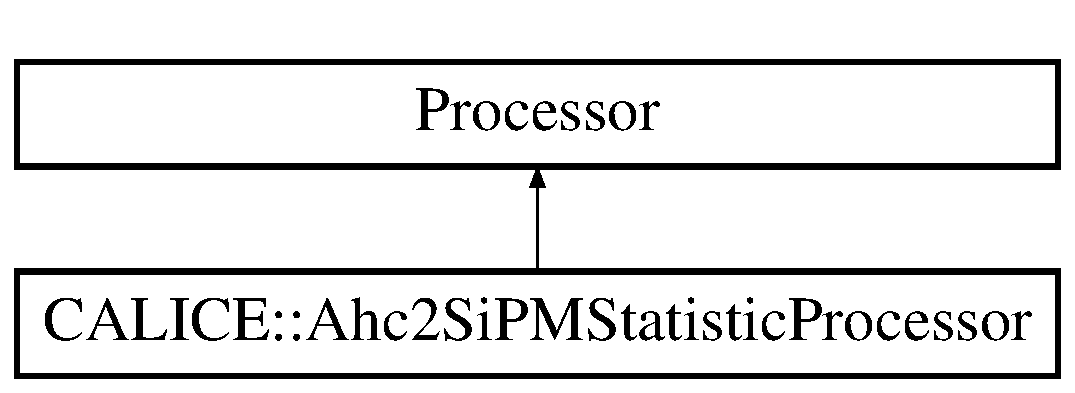
\includegraphics[height=2.000000cm]{classCALICE_1_1Ahc2SiPMStatisticProcessor}
\end{center}
\end{figure}
\subsection*{Public Member Functions}
\begin{DoxyCompactItemize}
\item 
virtual Processor $\ast$ {\bfseries new\-Processor} ()\label{classCALICE_1_1Ahc2SiPMStatisticProcessor_a5cdbdcc8e47117d48748d8cb74360424}

\item 
{\bf Ahc2\-Si\-P\-M\-Statistic\-Processor} ()\label{classCALICE_1_1Ahc2SiPMStatisticProcessor_ad4c7742312464d70b606da147004d605}

\begin{DoxyCompactList}\small\item\em Constructor. \end{DoxyCompactList}\item 
{\bf $\sim$\-Ahc2\-Si\-P\-M\-Statistic\-Processor} ()\label{classCALICE_1_1Ahc2SiPMStatisticProcessor_aad2ee5462a90fd49e0691d5030b7ca65}

\begin{DoxyCompactList}\small\item\em Destructor. \end{DoxyCompactList}\item 
virtual void {\bf init} ()\label{classCALICE_1_1Ahc2SiPMStatisticProcessor_a1a7b89745d394e9dd21ea63a9ec4a65d}

\begin{DoxyCompactList}\small\item\em Initialise. \end{DoxyCompactList}\item 
virtual void {\bf process\-Run\-Header} (L\-C\-Run\-Header $\ast$run)\label{classCALICE_1_1Ahc2SiPMStatisticProcessor_a7471c1f70ce311f477d65417eb0fc5c3}

\begin{DoxyCompactList}\small\item\em Process header. \end{DoxyCompactList}\item 
virtual void {\bf process\-Event} (L\-C\-Event $\ast$evt)\label{classCALICE_1_1Ahc2SiPMStatisticProcessor_a33f43727632ea28b5a7b2ede4b150b98}

\begin{DoxyCompactList}\small\item\em Process event (the working horse) \end{DoxyCompactList}\item 
virtual void {\bf check} (L\-C\-Event $\ast$evt)\label{classCALICE_1_1Ahc2SiPMStatisticProcessor_abea612c24758ae2a02567e2371997c40}

\begin{DoxyCompactList}\small\item\em Check. \end{DoxyCompactList}\item 
virtual void {\bf end} ()\label{classCALICE_1_1Ahc2SiPMStatisticProcessor_a8622faa7bfb96508f729051441dfd9b7}

\begin{DoxyCompactList}\small\item\em End of processing. \end{DoxyCompactList}\item 
virtual void {\bf print\-Parameters} ()\label{classCALICE_1_1Ahc2SiPMStatisticProcessor_a0c2c57c22063af53ee5254e8748ee235}

\begin{DoxyCompactList}\small\item\em Print Parameters. \end{DoxyCompactList}\end{DoxyCompactItemize}
\subsection*{Protected Member Functions}
\begin{DoxyCompactItemize}
\item 
void {\bf fill\-Container} (L\-C\-Collection $\ast$input\-Col)
\begin{DoxyCompactList}\small\item\em Fill a mapped container with the \doxyref{A\-H\-C\-A\-L}{p.}{namespaceCALICE_1_1AHCAL} cells. \end{DoxyCompactList}\item 
void {\bf simulate\-Optical\-Cross\-Talk} ()
\begin{DoxyCompactList}\small\item\em Simulate the optical cross-\/talk (i.\-e. \end{DoxyCompactList}\item 
void {\bf simulate\-Si\-P\-M\-Behaviour} ()\label{classCALICE_1_1Ahc2SiPMStatisticProcessor_a1ea294fe0b73c43d266d90b3fd53e814}

\begin{DoxyCompactList}\small\item\em Simulate the Si\-P\-M binomial behaviour. \end{DoxyCompactList}\item 
void {\bf add\-Noise} (L\-C\-Collection $\ast$noise\-Col)
\begin{DoxyCompactList}\small\item\em Add noise events from data. \end{DoxyCompactList}\item 
void {\bf create\-Output\-Collection} (L\-C\-Event $\ast$evt, const std\-::string col\-Name)
\begin{DoxyCompactList}\small\item\em Create output collection of digitised \doxyref{A\-H\-C\-A\-L}{p.}{namespaceCALICE_1_1AHCAL} hits. \end{DoxyCompactList}\end{DoxyCompactItemize}
\subsection*{Private Attributes}
\begin{DoxyCompactItemize}
\item 
std\-::string {\bf \-\_\-calorim\-Inp\-Collection}\label{classCALICE_1_1Ahc2SiPMStatisticProcessor_ad6530c343634aced1a4f4266a56dde52}

\begin{DoxyCompactList}\small\item\em input collection name \end{DoxyCompactList}\item 
std\-::string {\bf \-\_\-calorim\-Out\-Collection}\label{classCALICE_1_1Ahc2SiPMStatisticProcessor_a60e53201d752c229ae0c975705fbe788}

\begin{DoxyCompactList}\small\item\em output collection name \end{DoxyCompactList}\item 
vector$<$ std\-::string $>$ {\bf \-\_\-calorim\-Inp\-Collections}\label{classCALICE_1_1Ahc2SiPMStatisticProcessor_a6b0870b2c909736c0c309596c1fce428}

\begin{DoxyCompactList}\small\item\em input collection name \end{DoxyCompactList}\item 
vector$<$ std\-::string $>$ {\bf \-\_\-calorim\-Out\-Collections}\label{classCALICE_1_1Ahc2SiPMStatisticProcessor_a5fe5d1f4b1894ad2076869da5dda5596}

\begin{DoxyCompactList}\small\item\em output collection name \end{DoxyCompactList}\item 
std\-::string {\bf \-\_\-noise\-Col\-Name}\label{classCALICE_1_1Ahc2SiPMStatisticProcessor_a9f31e354c2eabd530855f62f167b9c3b}

\begin{DoxyCompactList}\small\item\em Noise collection name. \end{DoxyCompactList}\item 
std\-::string {\bf \-\_\-mapping\-Processor\-Name}\label{classCALICE_1_1Ahc2SiPMStatisticProcessor_a7e45dfe6f71626a4625267db08ddb37b}

\begin{DoxyCompactList}\small\item\em Mapping Processor Name. \end{DoxyCompactList}\item 
std\-::string {\bf \-\_\-cell\-Neighbours\-Processor\-Name}\label{classCALICE_1_1Ahc2SiPMStatisticProcessor_af07d7359686fceae4c364931c6fd2770}

\begin{DoxyCompactList}\small\item\em name of the processor which provides the cells neighbours \end{DoxyCompactList}\item 
std\-::string {\bf \-\_\-cell\-Description\-Processor\-Name}\label{classCALICE_1_1Ahc2SiPMStatisticProcessor_a98b7f1328a0ed947f7e4b214d8bf9a6d}

\begin{DoxyCompactList}\small\item\em Cell\-Description Processor name. \end{DoxyCompactList}\item 
std\-::string {\bf \-\_\-calib\-Processor\-Name}\label{classCALICE_1_1Ahc2SiPMStatisticProcessor_a1fab5b178e9d23ecbf4ef2e5c313e6b1}

\begin{DoxyCompactList}\small\item\em Calibration Processor Name. \end{DoxyCompactList}\item 
bool {\bf \-\_\-filter\-Dead\-Cells}\label{classCALICE_1_1Ahc2SiPMStatisticProcessor_a3d56d73f8743287f0c2193a6422816aa}

\begin{DoxyCompactList}\small\item\em filter dead cells \end{DoxyCompactList}\item 
bool {\bf \-\_\-do\-Mip\-Temp\-Corr}\label{classCALICE_1_1Ahc2SiPMStatisticProcessor_a5bfa570dd84ee9f442b7331c7ba0613f}

\begin{DoxyCompactList}\small\item\em do M\-I\-P temperature correction \end{DoxyCompactList}\item 
bool {\bf \-\_\-do\-Gain\-Temp\-Corr}\label{classCALICE_1_1Ahc2SiPMStatisticProcessor_a9b03e178918d2da408f338066339e681}

\begin{DoxyCompactList}\small\item\em do Gain temperature correction \end{DoxyCompactList}\item 
bool {\bf \-\_\-filter\-Default\-Cells}\label{classCALICE_1_1Ahc2SiPMStatisticProcessor_a104e829016f18843af1f2e24a1e0fe67}

\begin{DoxyCompactList}\small\item\em filter cells with default values \end{DoxyCompactList}\item 
bool {\bf \-\_\-do\-Saturation}\label{classCALICE_1_1Ahc2SiPMStatisticProcessor_a501fd0b4f0be7cc8b2f07e009c810723}

\begin{DoxyCompactList}\small\item\em do Si\-P\-M Saturation \end{DoxyCompactList}\item 
bool {\bf \-\_\-do\-Binomial\-Smearing}\label{classCALICE_1_1Ahc2SiPMStatisticProcessor_af1a2f795b7ee8a7ada9c2f3cbc46b1cb}

\begin{DoxyCompactList}\small\item\em do Binomial Smearing \end{DoxyCompactList}\item 
bool {\bf \-\_\-do\-Additional\-Smearing}\label{classCALICE_1_1Ahc2SiPMStatisticProcessor_ae5ab393998c69f316573f53d15d2e726}

\begin{DoxyCompactList}\small\item\em do additional Smearing \end{DoxyCompactList}\item 
bool {\bf \-\_\-do\-Add\-Noise}\label{classCALICE_1_1Ahc2SiPMStatisticProcessor_aba121a447270df73fe8e671ca646a072}

\begin{DoxyCompactList}\small\item\em Add Noise. \end{DoxyCompactList}\item 
float {\bf \-\_\-pix\-Spread}\label{classCALICE_1_1Ahc2SiPMStatisticProcessor_a524477012ed19fae02c7a8a3dfc98f5c}

\begin{DoxyCompactList}\small\item\em value in pixel spread \end{DoxyCompactList}\item 
bool {\bf \-\_\-correct\-Default\-Gain\-To\-L\-Y}\label{classCALICE_1_1Ahc2SiPMStatisticProcessor_a96b097630abf3c89a62ed0ed147834f2}

\begin{DoxyCompactList}\small\item\em Correct L\-Y if default gain. \end{DoxyCompactList}\item 
bool {\bf \-\_\-physics\-Mode}\label{classCALICE_1_1Ahc2SiPMStatisticProcessor_a11224fa3815f8ea0853176100b15a743}

\begin{DoxyCompactList}\small\item\em physics mode for new I\-T\-E\-P \end{DoxyCompactList}\item 
bool {\bf \-\_\-noise\-Energy\-M\-I\-P}\label{classCALICE_1_1Ahc2SiPMStatisticProcessor_a995e60f3eb2e0b01aafad937de175fb2}

\begin{DoxyCompactList}\small\item\em energy of noise hits are in M\-I\-P \end{DoxyCompactList}\item 
bool {\bf \-\_\-do\-Optical\-Cross\-Talk}\label{classCALICE_1_1Ahc2SiPMStatisticProcessor_a55138f5ef338a7e63d6aa5d86a4947b3}

\begin{DoxyCompactList}\small\item\em flag to disable/enable optical cross talk among neighbour tiles \end{DoxyCompactList}\item 
float {\bf \-\_\-fixed\-L\-Y}\label{classCALICE_1_1Ahc2SiPMStatisticProcessor_a20d4a2d56dd0bab777ad261f2dbbca6b}

\begin{DoxyCompactList}\small\item\em fix light yield if default gain \end{DoxyCompactList}\item 
String\-Vec {\bf \-\_\-light\-Leakage}\label{classCALICE_1_1Ahc2SiPMStatisticProcessor_a53b1d594f36a7fbaa24d9b39d23c15e9}

\begin{DoxyCompactList}\small\item\em light leakage factor vector \end{DoxyCompactList}\item 
std\-::map$<$ int, float $>$ {\bf m\-\_\-leakage}\label{classCALICE_1_1Ahc2SiPMStatisticProcessor_a0842cee9ffb02d1efb3fad1c6afe41c1}

\begin{DoxyCompactList}\small\item\em map containing ight leakage factor for each layer \end{DoxyCompactList}\item 
T\-Random3 $\ast$ {\bf \-\_\-random\-Generator}\label{classCALICE_1_1Ahc2SiPMStatisticProcessor_a9cb302dd9327d40a9e6817289e1f74b4}

\begin{DoxyCompactList}\small\item\em pointer to R\-O\-O\-Ts random generator for pixel statistics \end{DoxyCompactList}\item 
int {\bf \-\_\-random\-Seed}
\begin{DoxyCompactList}\small\item\em random seed for the random generator. \end{DoxyCompactList}\item 
std\-::string {\bf \-\_\-mokka\-Encoding\-String}\label{classCALICE_1_1Ahc2SiPMStatisticProcessor_aa02958354565b3d5ed9b449642984c48}

\begin{DoxyCompactList}\small\item\em the Mokka encoding string \end{DoxyCompactList}\item 
const Ahc2\-Mapper $\ast$ {\bf \-\_\-mapper}\label{classCALICE_1_1Ahc2SiPMStatisticProcessor_ad4e91d1ff807766f225acb8687f5c3eb}

\begin{DoxyCompactList}\small\item\em pointer to the used mapped \end{DoxyCompactList}\item 
unsigned int {\bf \-\_\-mapper\-Version}\label{classCALICE_1_1Ahc2SiPMStatisticProcessor_ad79e48205a744237759c542513956619}

\begin{DoxyCompactList}\small\item\em mapper version \end{DoxyCompactList}\item 
Mapped\-Container\\*
$<$ C\-A\-L\-I\-C\-E\-::\-Cell\-Description $>$ $\ast$ {\bf \-\_\-cell\-Descriptions}\label{classCALICE_1_1Ahc2SiPMStatisticProcessor_ab4db21c796e4acb08c76df5b180411b8}

\begin{DoxyCompactList}\small\item\em mapped container of cells description \end{DoxyCompactList}\item 
Mapped\-Container\\*
$<$ C\-A\-L\-I\-C\-E\-::\-Cell\-Neighbours $>$ $\ast$ {\bf \-\_\-cell\-Neighbours}\label{classCALICE_1_1Ahc2SiPMStatisticProcessor_aaa69b840289e408c755c0120b3fc84ad}

\begin{DoxyCompactList}\small\item\em mapped container of cells neighbours \end{DoxyCompactList}\item 
Mapped\-Container\\*
$<$ Ahc2\-Calibrations $>$ $\ast$ {\bf \-\_\-calib\-Container}\label{classCALICE_1_1Ahc2SiPMStatisticProcessor_a57b732c8fb88b7e1ee0402236b910c65}

\begin{DoxyCompactList}\small\item\em mapped container of Si\-P\-M calibrations \end{DoxyCompactList}\item 
Mapped\-Container\\*
$<$ Calorimeter\-Hit\-Impl $>$ $\ast$ {\bf \-\_\-\-Hit\-Container}\label{classCALICE_1_1Ahc2SiPMStatisticProcessor_a93b8261f0541bdb89fe3bd1c34a9bbb5}

\begin{DoxyCompactList}\small\item\em mapped container of \doxyref{A\-H\-C\-A\-L}{p.}{namespaceCALICE_1_1AHCAL} cells \end{DoxyCompactList}\item 
int {\bfseries \-\_\-n\-Run}\label{classCALICE_1_1Ahc2SiPMStatisticProcessor_aee588a97b13de6aa776b51638edccf6d}

\item 
int {\bfseries \-\_\-n\-Evt}\label{classCALICE_1_1Ahc2SiPMStatisticProcessor_a32f9509156a900a8206c47e3cacf4b07}

\end{DoxyCompactItemize}
\subsection*{Static Private Attributes}
\begin{DoxyCompactItemize}
\item 
static const unsigned int {\bf M\-A\-X\-A\-D\-C} = 4096\label{classCALICE_1_1Ahc2SiPMStatisticProcessor_a04a802ac94bbe8809bcb9f00debe998b}

\begin{DoxyCompactList}\small\item\em Max A\-D\-C for High Gain. \end{DoxyCompactList}\end{DoxyCompactItemize}


\subsection{Detailed Description}
Class for doing the \doxyref{A\-H\-C\-A\-L}{p.}{namespaceCALICE_1_1AHCAL} digitisation (Si\-P\-M treatment) 

\begin{DoxyAuthor}{Author}
{\tt eldwan.\-brianne@desy.\-de} 
\end{DoxyAuthor}
\begin{DoxyVersion}{Version}
1.\-0 
\end{DoxyVersion}
\begin{DoxyDate}{Date}
December 2015 
\end{DoxyDate}


Definition at line 43 of file Ahc2\-Si\-P\-M\-Statistic\-Processor.\-hh.



\subsection{Member Function Documentation}
\index{C\-A\-L\-I\-C\-E\-::\-Ahc2\-Si\-P\-M\-Statistic\-Processor@{C\-A\-L\-I\-C\-E\-::\-Ahc2\-Si\-P\-M\-Statistic\-Processor}!add\-Noise@{add\-Noise}}
\index{add\-Noise@{add\-Noise}!CALICE::Ahc2SiPMStatisticProcessor@{C\-A\-L\-I\-C\-E\-::\-Ahc2\-Si\-P\-M\-Statistic\-Processor}}
\subsubsection[{add\-Noise}]{\setlength{\rightskip}{0pt plus 5cm}void C\-A\-L\-I\-C\-E\-::\-Ahc2\-Si\-P\-M\-Statistic\-Processor\-::add\-Noise (
\begin{DoxyParamCaption}
\item[{L\-C\-Collection $\ast$}]{noise\-Col}
\end{DoxyParamCaption}
)\hspace{0.3cm}{\ttfamily [protected]}}\label{classCALICE_1_1Ahc2SiPMStatisticProcessor_aafa4b11452ff498ec4ef84dceeb93e6d}


Add noise events from data. 


\begin{DoxyParams}{Parameters}
{\em noise\-Col} & the noise collection \\
\hline
\end{DoxyParams}


Definition at line 791 of file Ahc2\-Si\-P\-M\-Statistic\-Processor.\-cc.



References \-\_\-calib\-Container, \-\_\-do\-Add\-Noise, \-\_\-do\-Saturation, \-\_\-\-Hit\-Container, \-\_\-mokka\-Encoding\-String, \-\_\-noise\-Energy\-M\-I\-P, and M\-A\-X\-A\-D\-C.



Referenced by process\-Event().

\index{C\-A\-L\-I\-C\-E\-::\-Ahc2\-Si\-P\-M\-Statistic\-Processor@{C\-A\-L\-I\-C\-E\-::\-Ahc2\-Si\-P\-M\-Statistic\-Processor}!create\-Output\-Collection@{create\-Output\-Collection}}
\index{create\-Output\-Collection@{create\-Output\-Collection}!CALICE::Ahc2SiPMStatisticProcessor@{C\-A\-L\-I\-C\-E\-::\-Ahc2\-Si\-P\-M\-Statistic\-Processor}}
\subsubsection[{create\-Output\-Collection}]{\setlength{\rightskip}{0pt plus 5cm}void C\-A\-L\-I\-C\-E\-::\-Ahc2\-Si\-P\-M\-Statistic\-Processor\-::create\-Output\-Collection (
\begin{DoxyParamCaption}
\item[{L\-C\-Event $\ast$}]{evt, }
\item[{const std\-::string}]{col\-Name}
\end{DoxyParamCaption}
)\hspace{0.3cm}{\ttfamily [protected]}}\label{classCALICE_1_1Ahc2SiPMStatisticProcessor_a72667f16ab7399f08fd1bdfb8b394234}


Create output collection of digitised \doxyref{A\-H\-C\-A\-L}{p.}{namespaceCALICE_1_1AHCAL} hits. 


\begin{DoxyParams}{Parameters}
{\em evt} & L\-C\-Event to which the collection will be added \\
\hline
{\em col\-Name} & name of the output collection \\
\hline
\end{DoxyParams}


Definition at line 870 of file Ahc2\-Si\-P\-M\-Statistic\-Processor.\-cc.



References \-\_\-\-Hit\-Container, and \-\_\-mokka\-Encoding\-String.



Referenced by process\-Event().

\index{C\-A\-L\-I\-C\-E\-::\-Ahc2\-Si\-P\-M\-Statistic\-Processor@{C\-A\-L\-I\-C\-E\-::\-Ahc2\-Si\-P\-M\-Statistic\-Processor}!fill\-Container@{fill\-Container}}
\index{fill\-Container@{fill\-Container}!CALICE::Ahc2SiPMStatisticProcessor@{C\-A\-L\-I\-C\-E\-::\-Ahc2\-Si\-P\-M\-Statistic\-Processor}}
\subsubsection[{fill\-Container}]{\setlength{\rightskip}{0pt plus 5cm}void C\-A\-L\-I\-C\-E\-::\-Ahc2\-Si\-P\-M\-Statistic\-Processor\-::fill\-Container (
\begin{DoxyParamCaption}
\item[{L\-C\-Collection $\ast$}]{input\-Col}
\end{DoxyParamCaption}
)\hspace{0.3cm}{\ttfamily [protected]}}\label{classCALICE_1_1Ahc2SiPMStatisticProcessor_a7fa64a083d999a8cdb7660cd5d0289af}


Fill a mapped container with the \doxyref{A\-H\-C\-A\-L}{p.}{namespaceCALICE_1_1AHCAL} cells. 


\begin{DoxyParams}{Parameters}
{\em input\-Col} & the input collection, with the \doxyref{A\-H\-C\-A\-L}{p.}{namespaceCALICE_1_1AHCAL} Mokka hits \\
\hline
\end{DoxyParams}


Definition at line 358 of file Ahc2\-Si\-P\-M\-Statistic\-Processor.\-cc.



References \-\_\-\-Hit\-Container, \-\_\-mapper, and \-\_\-mokka\-Encoding\-String.



Referenced by process\-Event().

\index{C\-A\-L\-I\-C\-E\-::\-Ahc2\-Si\-P\-M\-Statistic\-Processor@{C\-A\-L\-I\-C\-E\-::\-Ahc2\-Si\-P\-M\-Statistic\-Processor}!simulate\-Optical\-Cross\-Talk@{simulate\-Optical\-Cross\-Talk}}
\index{simulate\-Optical\-Cross\-Talk@{simulate\-Optical\-Cross\-Talk}!CALICE::Ahc2SiPMStatisticProcessor@{C\-A\-L\-I\-C\-E\-::\-Ahc2\-Si\-P\-M\-Statistic\-Processor}}
\subsubsection[{simulate\-Optical\-Cross\-Talk}]{\setlength{\rightskip}{0pt plus 5cm}void C\-A\-L\-I\-C\-E\-::\-Ahc2\-Si\-P\-M\-Statistic\-Processor\-::simulate\-Optical\-Cross\-Talk (
\begin{DoxyParamCaption}
{}
\end{DoxyParamCaption}
)\hspace{0.3cm}{\ttfamily [protected]}}\label{classCALICE_1_1Ahc2SiPMStatisticProcessor_afa269ae00bbf2f185e154a0464bf972d}


Simulate the optical cross-\/talk (i.\-e. 

light leakage) between the tiles 

Definition at line 406 of file Ahc2\-Si\-P\-M\-Statistic\-Processor.\-cc.



References \-\_\-cell\-Descriptions, \-\_\-cell\-Neighbours, \-\_\-cell\-Neighbours\-Processor\-Name, \-\_\-\-Hit\-Container, \-\_\-mokka\-Encoding\-String, and m\-\_\-leakage.



Referenced by process\-Event().



\subsection{Field Documentation}
\index{C\-A\-L\-I\-C\-E\-::\-Ahc2\-Si\-P\-M\-Statistic\-Processor@{C\-A\-L\-I\-C\-E\-::\-Ahc2\-Si\-P\-M\-Statistic\-Processor}!\-\_\-random\-Seed@{\-\_\-random\-Seed}}
\index{\-\_\-random\-Seed@{\-\_\-random\-Seed}!CALICE::Ahc2SiPMStatisticProcessor@{C\-A\-L\-I\-C\-E\-::\-Ahc2\-Si\-P\-M\-Statistic\-Processor}}
\subsubsection[{\-\_\-random\-Seed}]{\setlength{\rightskip}{0pt plus 5cm}int C\-A\-L\-I\-C\-E\-::\-Ahc2\-Si\-P\-M\-Statistic\-Processor\-::\-\_\-random\-Seed\hspace{0.3cm}{\ttfamily [private]}}\label{classCALICE_1_1Ahc2SiPMStatisticProcessor_ac53cdf42123fe76fe1e633fb923652ab}


random seed for the random generator. 

Steerable. 

Definition at line 141 of file Ahc2\-Si\-P\-M\-Statistic\-Processor.\-hh.



Referenced by Ahc2\-Si\-P\-M\-Statistic\-Processor(), and init().



The documentation for this class was generated from the following files\-:\begin{DoxyCompactItemize}
\item 
Ahc2\-Si\-P\-M\-Statistic\-Processor.\-hh\item 
Ahc2\-Si\-P\-M\-Statistic\-Processor.\-cc\end{DoxyCompactItemize}

\section{C\-A\-L\-I\-C\-E\-:\-:Ahc2\-Time\-Smearing\-Processor Class Reference}
\label{classCALICE_1_1Ahc2TimeSmearingProcessor}\index{C\-A\-L\-I\-C\-E\-::\-Ahc2\-Time\-Smearing\-Processor@{C\-A\-L\-I\-C\-E\-::\-Ahc2\-Time\-Smearing\-Processor}}


Class for doing the \doxyref{A\-H\-C\-A\-L}{p.}{namespaceCALICE_1_1AHCAL} digitisation (Time Smearing)  




{\ttfamily \#include $<$Ahc2\-Time\-Smearing\-Processor.\-hh$>$}

Inheritance diagram for C\-A\-L\-I\-C\-E\-:\-:Ahc2\-Time\-Smearing\-Processor\-:\begin{figure}[H]
\begin{center}
\leavevmode
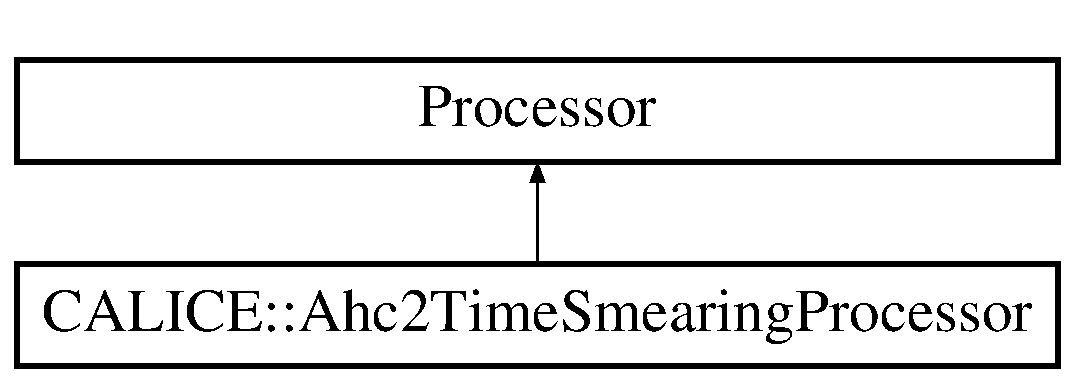
\includegraphics[height=2.000000cm]{classCALICE_1_1Ahc2TimeSmearingProcessor}
\end{center}
\end{figure}
\subsection*{Public Member Functions}
\begin{DoxyCompactItemize}
\item 
virtual Processor $\ast$ {\bfseries new\-Processor} ()\label{classCALICE_1_1Ahc2TimeSmearingProcessor_aee39c56a0c8b2630ebb8b026028d45e1}

\item 
{\bf Ahc2\-Time\-Smearing\-Processor} ()\label{classCALICE_1_1Ahc2TimeSmearingProcessor_a33047e2c438f270c6912579711e95884}

\begin{DoxyCompactList}\small\item\em Constructor. \end{DoxyCompactList}\item 
{\bf $\sim$\-Ahc2\-Time\-Smearing\-Processor} ()\label{classCALICE_1_1Ahc2TimeSmearingProcessor_add1d7fba8570dcf282d2b47252f6463a}

\begin{DoxyCompactList}\small\item\em Destructor. \end{DoxyCompactList}\item 
virtual void {\bf init} ()\label{classCALICE_1_1Ahc2TimeSmearingProcessor_a6753a3323e61c61e40495b7f4615189a}

\begin{DoxyCompactList}\small\item\em Initialise. \end{DoxyCompactList}\item 
virtual void {\bf process\-Run\-Header} (L\-C\-Run\-Header $\ast$run)\label{classCALICE_1_1Ahc2TimeSmearingProcessor_a70ef7905e600a36a51568b096aec4ce9}

\begin{DoxyCompactList}\small\item\em Process header. \end{DoxyCompactList}\item 
virtual void {\bf process\-Event} (L\-C\-Event $\ast$evt)\label{classCALICE_1_1Ahc2TimeSmearingProcessor_ad6eb1ede3d5c9ae6bf6f81e1481ee1dc}

\begin{DoxyCompactList}\small\item\em Process event (the working horse) \end{DoxyCompactList}\item 
virtual void {\bf check} (L\-C\-Event $\ast$evt)\label{classCALICE_1_1Ahc2TimeSmearingProcessor_a3e2fa3d476464e277a155fe718ddf2f8}

\begin{DoxyCompactList}\small\item\em Check. \end{DoxyCompactList}\item 
virtual void {\bf end} ()\label{classCALICE_1_1Ahc2TimeSmearingProcessor_a148f43677d0ff3aa9bd40916da4114ad}

\begin{DoxyCompactList}\small\item\em End of processing. \end{DoxyCompactList}\item 
virtual void {\bf print\-Parameters} ()\label{classCALICE_1_1Ahc2TimeSmearingProcessor_a620da82aee6a75c88446f9c875b7a47c}

\begin{DoxyCompactList}\small\item\em Print Parameters. \end{DoxyCompactList}\item 
void {\bf Fill\-Container} (L\-C\-Event $\ast$evt)\label{classCALICE_1_1Ahc2TimeSmearingProcessor_a213695d36a37a0ba1fbb809b95be4de9}

\begin{DoxyCompactList}\small\item\em Hardware Connection. \end{DoxyCompactList}\end{DoxyCompactItemize}
\subsection*{Private Attributes}
\begin{DoxyCompactItemize}
\item 
std\-::string {\bf \-\_\-calorim\-Inp\-Collection}\label{classCALICE_1_1Ahc2TimeSmearingProcessor_a8553fe50d704d79ef994b4179171ae83}

\begin{DoxyCompactList}\small\item\em input collection name \end{DoxyCompactList}\item 
std\-::string {\bf \-\_\-calorim\-Out\-Collection}\label{classCALICE_1_1Ahc2TimeSmearingProcessor_a1ff8ef5c34a0afd7e30aeaabd331da2b}

\begin{DoxyCompactList}\small\item\em output collection name \end{DoxyCompactList}\item 
vector$<$ std\-::string $>$ {\bf \-\_\-calorim\-Inp\-Collections}\label{classCALICE_1_1Ahc2TimeSmearingProcessor_ad8d306dee8ff9e77f33db04e7c5b5533}

\begin{DoxyCompactList}\small\item\em input collection name \end{DoxyCompactList}\item 
vector$<$ std\-::string $>$ {\bf \-\_\-calorim\-Out\-Collections}\label{classCALICE_1_1Ahc2TimeSmearingProcessor_a6e996f04572594f0f7bf27753a109cd5}

\begin{DoxyCompactList}\small\item\em output collection name \end{DoxyCompactList}\item 
bool {\bf \-\_\-do\-Time\-Smearing}\label{classCALICE_1_1Ahc2TimeSmearingProcessor_a62235a91d7cbd9fa985cda87cd47ec8a}

\begin{DoxyCompactList}\small\item\em do Time\-Smearing \end{DoxyCompactList}\item 
float {\bfseries \-\_\-time\-Smearing}\label{classCALICE_1_1Ahc2TimeSmearingProcessor_a2a5a1c1e6e3229c1e954e7b231d85894}

\item 
bool {\bf \-\_\-do\-To\-F\-Shift}\label{classCALICE_1_1Ahc2TimeSmearingProcessor_a39d61eefd9e94d9662fe1345799e79f7}

\begin{DoxyCompactList}\small\item\em do shift layers by time of flight \end{DoxyCompactList}\item 
T\-Random3 $\ast$ {\bf \-\_\-random\-Generator}\label{classCALICE_1_1Ahc2TimeSmearingProcessor_a23fdda0b3cbc3a7347ac7c200c84cff4}

\begin{DoxyCompactList}\small\item\em pointer to R\-O\-O\-Ts random generator for gaussian smearing \end{DoxyCompactList}\item 
int {\bf \-\_\-random\-Seed}
\begin{DoxyCompactList}\small\item\em random seed for the random generator. \end{DoxyCompactList}\item 
std\-::string {\bf \-\_\-mokka\-Encoding\-String}\label{classCALICE_1_1Ahc2TimeSmearingProcessor_a2b85ba6e582f4a0b07ae8eab09e27440}

\begin{DoxyCompactList}\small\item\em the Mokka encoding string \end{DoxyCompactList}\item 
int {\bfseries \-\_\-n\-Run}\label{classCALICE_1_1Ahc2TimeSmearingProcessor_a3000c79d829b8b73ca7c4ce114da2d51}

\item 
int {\bfseries \-\_\-n\-Evt}\label{classCALICE_1_1Ahc2TimeSmearingProcessor_af8f690d9bc9acb4d1e00556aede9aadf}

\item 
std\-::string {\bf \-\_\-mapping\-Processor\-Name}\label{classCALICE_1_1Ahc2TimeSmearingProcessor_aed37f0b8fe83aa5a4073a4f33ef36cc7}

\begin{DoxyCompactList}\small\item\em name of the processor which provides the mapping \end{DoxyCompactList}\item 
const Ahc2\-Mapper $\ast$ {\bf \-\_\-mapper}\label{classCALICE_1_1Ahc2TimeSmearingProcessor_a8683e0125515b0614fa946a05e6d7bfd}

\begin{DoxyCompactList}\small\item\em the mapper \end{DoxyCompactList}\end{DoxyCompactItemize}


\subsection{Detailed Description}
Class for doing the \doxyref{A\-H\-C\-A\-L}{p.}{namespaceCALICE_1_1AHCAL} digitisation (Time Smearing) 

\begin{DoxyAuthor}{Author}
{\tt eldwan.\-brianne@desy.\-de} 
\end{DoxyAuthor}
\begin{DoxyVersion}{Version}
1.\-0 
\end{DoxyVersion}
\begin{DoxyDate}{Date}
July 2016 
\end{DoxyDate}


Definition at line 43 of file Ahc2\-Time\-Smearing\-Processor.\-hh.



\subsection{Field Documentation}
\index{C\-A\-L\-I\-C\-E\-::\-Ahc2\-Time\-Smearing\-Processor@{C\-A\-L\-I\-C\-E\-::\-Ahc2\-Time\-Smearing\-Processor}!\-\_\-random\-Seed@{\-\_\-random\-Seed}}
\index{\-\_\-random\-Seed@{\-\_\-random\-Seed}!CALICE::Ahc2TimeSmearingProcessor@{C\-A\-L\-I\-C\-E\-::\-Ahc2\-Time\-Smearing\-Processor}}
\subsubsection[{\-\_\-random\-Seed}]{\setlength{\rightskip}{0pt plus 5cm}int C\-A\-L\-I\-C\-E\-::\-Ahc2\-Time\-Smearing\-Processor\-::\-\_\-random\-Seed\hspace{0.3cm}{\ttfamily [private]}}\label{classCALICE_1_1Ahc2TimeSmearingProcessor_a95eff3ff1307d2f3d304a6e9a66b4a5d}


random seed for the random generator. 

Steerable. 

Definition at line 98 of file Ahc2\-Time\-Smearing\-Processor.\-hh.



Referenced by Ahc2\-Time\-Smearing\-Processor(), and init().



The documentation for this class was generated from the following files\-:\begin{DoxyCompactItemize}
\item 
Ahc2\-Time\-Smearing\-Processor.\-hh\item 
Ahc2\-Time\-Smearing\-Processor.\-cc\end{DoxyCompactItemize}

\section{C\-A\-L\-I\-C\-E\-:\-:Ahc2\-Trigger\-Bits Class Reference}
\label{classCALICE_1_1Ahc2TriggerBits}\index{C\-A\-L\-I\-C\-E\-::\-Ahc2\-Trigger\-Bits@{C\-A\-L\-I\-C\-E\-::\-Ahc2\-Trigger\-Bits}}


A small class which allow for the easy analysis of core trigger information.  




{\ttfamily \#include $<$Ahc2\-Trigger\-Sim.\-hh$>$}

Inheritance diagram for C\-A\-L\-I\-C\-E\-:\-:Ahc2\-Trigger\-Bits\-:\begin{figure}[H]
\begin{center}
\leavevmode
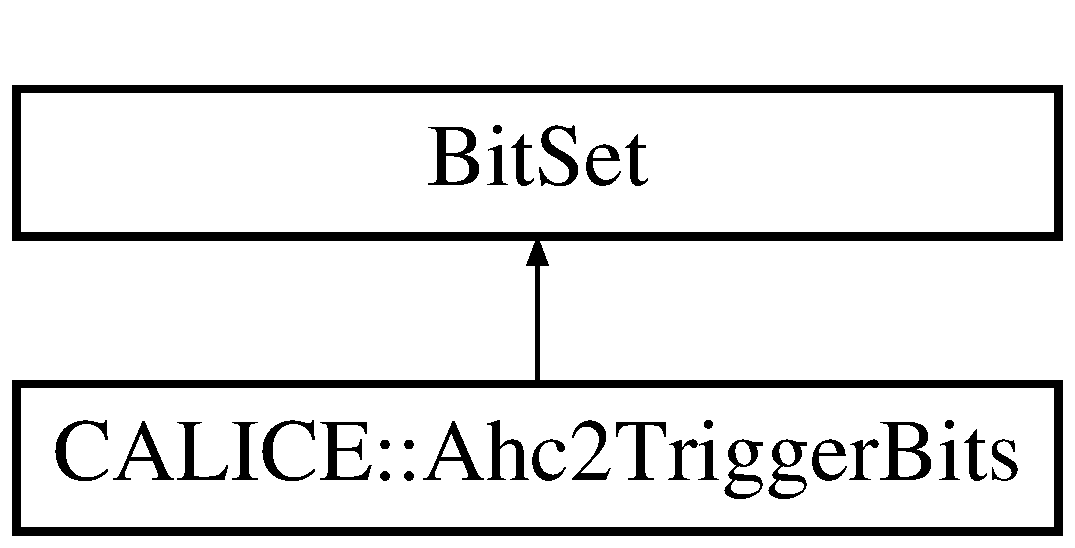
\includegraphics[height=2.000000cm]{classCALICE_1_1Ahc2TriggerBits}
\end{center}
\end{figure}
\subsection*{Public Types}
\begin{DoxyCompactItemize}
\item 
enum {\bfseries E\-Ahc2\-Trigger\-Bits\-No} \{ \\*
{\bfseries k\-S\-C1\-\_\-100x100}, 
{\bfseries k\-S\-C2\-\_\-100x100}, 
{\bfseries k\-S\-C1\-\_\-500x500}, 
{\bfseries k\-S\-C2\-\_\-500x500}, 
\\*
{\bfseries k\-Beam}, 
{\bfseries k\-No\-Triggers}
 \}
\end{DoxyCompactItemize}
\subsection*{Public Member Functions}
\begin{DoxyCompactItemize}
\item 
{\bfseries Ahc2\-Trigger\-Bits} (const int trigger\-\_\-bits)\label{classCALICE_1_1Ahc2TriggerBits_a89ad730200f80e923e0ec08181568a14}

\item 
void {\bfseries set\-Beam\-Trigger} (const bool state=true)\label{classCALICE_1_1Ahc2TriggerBits_a968dc35e8fd8e6cb9d421e98f9265db5}

\item 
void {\bfseries set\-Sc1\-\_\-100x100} (const bool state=true)\label{classCALICE_1_1Ahc2TriggerBits_a07d1b59ef322255420f02296ad1a449b}

\item 
void {\bfseries set\-Sc2\-\_\-100x100} (const bool state=true)\label{classCALICE_1_1Ahc2TriggerBits_a4d808a2272ce45333088a8b622b339a4}

\item 
void {\bfseries set\-Sc1\-\_\-500x500} (const bool state=true)\label{classCALICE_1_1Ahc2TriggerBits_a867edfd10460deeb66dcb597b62cc5f9}

\item 
void {\bfseries set\-Sc2\-\_\-500x500} (const bool state=true)\label{classCALICE_1_1Ahc2TriggerBits_aa6e7caf3a22c7ba80494c0b0bf819946}

\item 
bool {\bfseries is\-Beam\-Trigger} () const \label{classCALICE_1_1Ahc2TriggerBits_a6ddabf7d7159fbdb161ef5771df58d0b}

\item 
bool {\bfseries is\-Sc1\-\_\-100x100} () const \label{classCALICE_1_1Ahc2TriggerBits_ae40cacdbfe09dd9f8a1671be90ce06d6}

\item 
bool {\bfseries is\-Sc2\-\_\-100x100} () const \label{classCALICE_1_1Ahc2TriggerBits_a701f7ea3424da265e127bc256e86662c}

\item 
bool {\bfseries is\-Sc1\-\_\-500x500} () const \label{classCALICE_1_1Ahc2TriggerBits_aa0b8216333443b92de1a00fdf6e6b32a}

\item 
bool {\bfseries is\-Sc2\-\_\-500x500} () const \label{classCALICE_1_1Ahc2TriggerBits_a6f621752d5d0e0786bb8976548da8c25}

\end{DoxyCompactItemize}


\subsection{Detailed Description}
A small class which allow for the easy analysis of core trigger information. 

It allows the user to test which trigger was set in a given event. The information has to be shipped as an event parameter. \begin{DoxyAuthor}{Author}
{\tt eldwan.\-brianne@desy.\-de} 
\end{DoxyAuthor}
\begin{DoxyVersion}{Version}
1.\-0 
\end{DoxyVersion}
\begin{DoxyDate}{Date}
January 2017 
\end{DoxyDate}


Definition at line 96 of file Ahc2\-Trigger\-Sim.\-hh.



The documentation for this class was generated from the following file\-:\begin{DoxyCompactItemize}
\item 
Ahc2\-Trigger\-Sim.\-hh\end{DoxyCompactItemize}

\section{C\-A\-L\-I\-C\-E\-:\-:Ahc2\-Triggered\-Channels Class Reference}
\label{classCALICE_1_1Ahc2TriggeredChannels}\index{C\-A\-L\-I\-C\-E\-::\-Ahc2\-Triggered\-Channels@{C\-A\-L\-I\-C\-E\-::\-Ahc2\-Triggered\-Channels}}


Class for counting the number of triggered channels per Chip (rejecting dead channels) used for time smearing.  




{\ttfamily \#include $<$Ahc2\-Triggered\-Channels.\-hh$>$}

Inheritance diagram for C\-A\-L\-I\-C\-E\-:\-:Ahc2\-Triggered\-Channels\-:\begin{figure}[H]
\begin{center}
\leavevmode
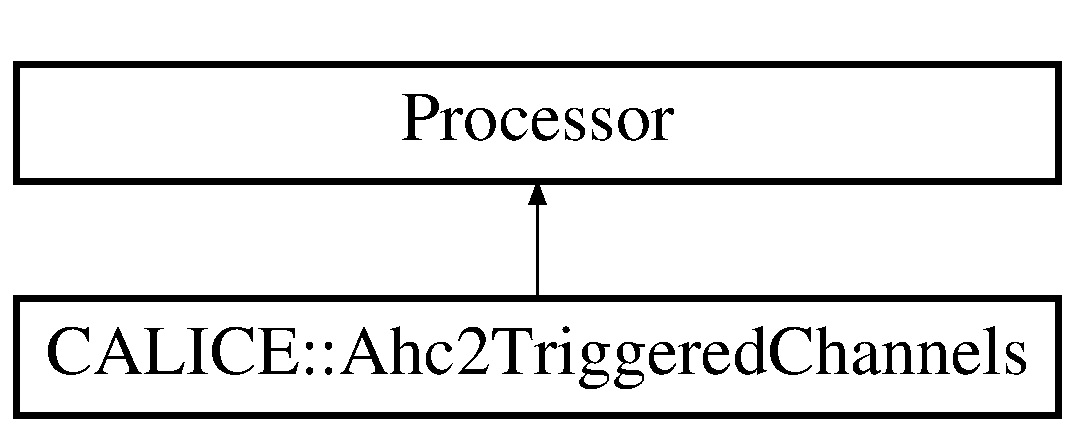
\includegraphics[height=2.000000cm]{classCALICE_1_1Ahc2TriggeredChannels}
\end{center}
\end{figure}
\subsection*{Public Member Functions}
\begin{DoxyCompactItemize}
\item 
virtual Processor $\ast$ {\bfseries new\-Processor} ()\label{classCALICE_1_1Ahc2TriggeredChannels_a5dbc7143416c6a9105d4f0cde5cb663c}

\item 
{\bf Ahc2\-Triggered\-Channels} ()\label{classCALICE_1_1Ahc2TriggeredChannels_ae335b3372bd597849b7a36feb252de57}

\begin{DoxyCompactList}\small\item\em Constructor. \end{DoxyCompactList}\item 
{\bf $\sim$\-Ahc2\-Triggered\-Channels} ()\label{classCALICE_1_1Ahc2TriggeredChannels_a97364f50d9ee2398bac43362b20ce35d}

\begin{DoxyCompactList}\small\item\em Destructor. \end{DoxyCompactList}\item 
virtual void {\bf init} ()\label{classCALICE_1_1Ahc2TriggeredChannels_ab1480e85ecfefd73ecbf31e2defb3f9e}

\begin{DoxyCompactList}\small\item\em Initialise. \end{DoxyCompactList}\item 
virtual void {\bf process\-Run\-Header} (L\-C\-Run\-Header $\ast$run)\label{classCALICE_1_1Ahc2TriggeredChannels_a98fc8cd1bf9f7e259fc8829c6ddb13df}

\begin{DoxyCompactList}\small\item\em Process header. \end{DoxyCompactList}\item 
virtual void {\bf process\-Event} (L\-C\-Event $\ast$evt)\label{classCALICE_1_1Ahc2TriggeredChannels_a22b08792663ee91bcdf0b0a1787a3282}

\begin{DoxyCompactList}\small\item\em Process event (the working horse) \end{DoxyCompactList}\item 
virtual void {\bf check} (L\-C\-Event $\ast$evt)\label{classCALICE_1_1Ahc2TriggeredChannels_a229ebbf2ec8d18654edaca15f0636e38}

\begin{DoxyCompactList}\small\item\em Check. \end{DoxyCompactList}\item 
virtual void {\bf end} ()\label{classCALICE_1_1Ahc2TriggeredChannels_a2679e163d4ccf1caea0b41a88676e419}

\begin{DoxyCompactList}\small\item\em End of processing. \end{DoxyCompactList}\end{DoxyCompactItemize}
\subsection*{Protected Attributes}
\begin{DoxyCompactItemize}
\item 
std\-::string {\bf \-\_\-calorim\-Inp\-Collection}\label{classCALICE_1_1Ahc2TriggeredChannels_a19d95908c195bb589969afd9d048f6a7}

\begin{DoxyCompactList}\small\item\em input collection name \end{DoxyCompactList}\item 
std\-::string {\bf \-\_\-calorim\-Out\-Collection}\label{classCALICE_1_1Ahc2TriggeredChannels_a294266c133fee81756d0f9527674bfd0}

\begin{DoxyCompactList}\small\item\em output collection name \end{DoxyCompactList}\item 
std\-::string {\bf \-\_\-mapping\-Processor\-Name}\label{classCALICE_1_1Ahc2TriggeredChannels_a2f22fbbf8a80f45c129b0f320de3ab3f}

\begin{DoxyCompactList}\small\item\em name of the processor which provides the mapping \end{DoxyCompactList}\item 
std\-::string {\bfseries \-\_\-encoding}\label{classCALICE_1_1Ahc2TriggeredChannels_a319667772397941987ed6bc4076b224f}

\item 
int {\bf \-\_\-n\-Run}\label{classCALICE_1_1Ahc2TriggeredChannels_acabca64049bc0ceadd8df49e73296e57}

\begin{DoxyCompactList}\small\item\em run number \end{DoxyCompactList}\item 
int {\bf \-\_\-n\-Evt}\label{classCALICE_1_1Ahc2TriggeredChannels_a5aa48858e4e0f6c4c0dc055b103181d0}

\begin{DoxyCompactList}\small\item\em event number \end{DoxyCompactList}\item 
const Ahc2\-Mapper $\ast$ {\bf \-\_\-mapper}\label{classCALICE_1_1Ahc2TriggeredChannels_a793ad95889916074bce275e4671f58b5}

\begin{DoxyCompactList}\small\item\em the mapper \end{DoxyCompactList}\item 
std\-::map$<$ int, int $>$ {\bf m\-\_\-\-Chip\-Trigger}\label{classCALICE_1_1Ahc2TriggeredChannels_a5f84dbcf33ef3f3ffb49b0877e6c7e42}

\begin{DoxyCompactList}\small\item\em map with number of triggered channels per chip for pedestal shift \end{DoxyCompactList}\item 
Int\-Vec {\bf n\-Hits\-Per\-Chip\-Above\-Thr}\label{classCALICE_1_1Ahc2TriggeredChannels_a417a5839a46ab815251b3cea17efb0a0}

\begin{DoxyCompactList}\small\item\em vector to store the number of hits per Chips per event \end{DoxyCompactList}\end{DoxyCompactItemize}


\subsection{Detailed Description}
Class for counting the number of triggered channels per Chip (rejecting dead channels) used for time smearing. 

\begin{DoxyAuthor}{Author}
{\tt eldwan.\-brianne@desy.\-de} 
\end{DoxyAuthor}
\begin{DoxyVersion}{Version}
2.\-0 
\end{DoxyVersion}
\begin{DoxyDate}{Date}
November 2016 
\end{DoxyDate}


Definition at line 32 of file Ahc2\-Triggered\-Channels.\-hh.



The documentation for this class was generated from the following files\-:\begin{DoxyCompactItemize}
\item 
Ahc2\-Triggered\-Channels.\-hh\item 
Ahc2\-Triggered\-Channels.\-cpp\end{DoxyCompactItemize}

\section{C\-A\-L\-I\-C\-E\-:\-:Ahc2\-Trigger\-Sim Class Reference}
\label{classCALICE_1_1Ahc2TriggerSim}\index{C\-A\-L\-I\-C\-E\-::\-Ahc2\-Trigger\-Sim@{C\-A\-L\-I\-C\-E\-::\-Ahc2\-Trigger\-Sim}}


Class for setting trigger bits in the event for M\-C.  




{\ttfamily \#include $<$Ahc2\-Trigger\-Sim.\-hh$>$}

Inheritance diagram for C\-A\-L\-I\-C\-E\-:\-:Ahc2\-Trigger\-Sim\-:\begin{figure}[H]
\begin{center}
\leavevmode
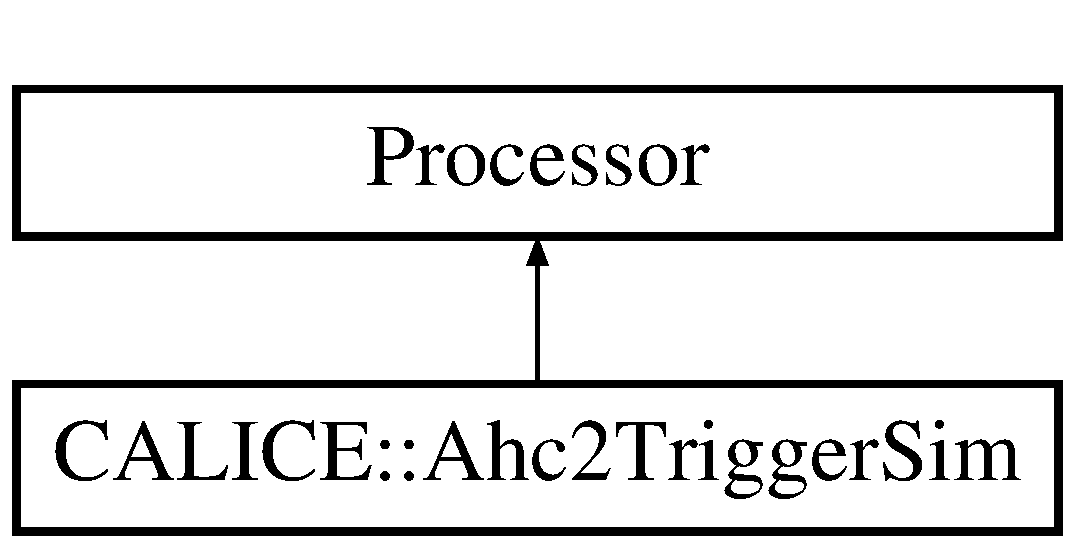
\includegraphics[height=2.000000cm]{classCALICE_1_1Ahc2TriggerSim}
\end{center}
\end{figure}
\subsection*{Public Member Functions}
\begin{DoxyCompactItemize}
\item 
virtual Processor $\ast$ {\bfseries new\-Processor} ()\label{classCALICE_1_1Ahc2TriggerSim_a908c333749d8847017189ebeccc67f36}

\item 
{\bf Ahc2\-Trigger\-Sim} ()\label{classCALICE_1_1Ahc2TriggerSim_a1c994c4a99a30d71da81baaf73d709e7}

\begin{DoxyCompactList}\small\item\em Constructor. \end{DoxyCompactList}\item 
{\bf $\sim$\-Ahc2\-Trigger\-Sim} ()\label{classCALICE_1_1Ahc2TriggerSim_ad40eb8e475c728e4be82ea48018f85ca}

\begin{DoxyCompactList}\small\item\em Destructor. \end{DoxyCompactList}\item 
virtual void {\bf init} ()\label{classCALICE_1_1Ahc2TriggerSim_a037a2ce2ab0d11398dea77f8b998f05e}

\begin{DoxyCompactList}\small\item\em Initialise. \end{DoxyCompactList}\item 
virtual void {\bf process\-Run\-Header} (L\-C\-Run\-Header $\ast$run)\label{classCALICE_1_1Ahc2TriggerSim_a4aa0642673b0742092bd2f9a4ba43550}

\begin{DoxyCompactList}\small\item\em Process header. \end{DoxyCompactList}\item 
virtual void {\bf process\-Event} (L\-C\-Event $\ast$evt)\label{classCALICE_1_1Ahc2TriggerSim_a652e15f9aac83ecd3f80f347f0b4d8d7}

\begin{DoxyCompactList}\small\item\em Process event (the working horse) \end{DoxyCompactList}\item 
virtual void {\bf check} (L\-C\-Event $\ast$evt)\label{classCALICE_1_1Ahc2TriggerSim_a3e23709a27312703b0ef9f7f1dd70ddf}

\begin{DoxyCompactList}\small\item\em Check. \end{DoxyCompactList}\item 
virtual void {\bf end} ()\label{classCALICE_1_1Ahc2TriggerSim_a60551290571f36baac32e08f2c0db082}

\begin{DoxyCompactList}\small\item\em End of processing. \end{DoxyCompactList}\item 
virtual void {\bf print\-Parameters} ()\label{classCALICE_1_1Ahc2TriggerSim_afc31cd3417220e2d4c21db6c41fec3f8}

\begin{DoxyCompactList}\small\item\em Print Parameters. \end{DoxyCompactList}\end{DoxyCompactItemize}
\subsection*{Protected Types}
\begin{DoxyCompactItemize}
\item 
enum {\bf E\-Trigger\-Sim\-Mode} \{ {\bf k\-Sim\-Trigger\-Mode100x100\-Coincidence} =1, 
{\bf k\-Sim\-Trigger\-Mode500x500\-Coincidence} =2
 \}
\end{DoxyCompactItemize}
\subsection*{Protected Attributes}
\begin{DoxyCompactItemize}
\item 
{\bf E\-Trigger\-Sim\-Mode} {\bfseries \-\_\-sim\-Trigger\-Mode}\label{classCALICE_1_1Ahc2TriggerSim_a9ae476f2767aac3277f781e47e356643}

\item 
int {\bfseries \-\_\-sim\-Trigger\-Mode\-Parameter}\label{classCALICE_1_1Ahc2TriggerSim_a579a9908f65019aec5435ec3c8c4006f}

\item 
int {\bf \-\_\-n\-Sc1\-\_\-100x100}\label{classCALICE_1_1Ahc2TriggerSim_af0b85f62b857567d2ad97362ad867944}

\begin{DoxyCompactList}\small\item\em number of events passing through the scintillator 100x100 S\-C1 \end{DoxyCompactList}\item 
int {\bf \-\_\-n\-Sc2\-\_\-100x100}\label{classCALICE_1_1Ahc2TriggerSim_a62c9633a37533c1454a674227e1adbfe}

\begin{DoxyCompactList}\small\item\em number of events passing through the scintillator 100x100 S\-C2 \end{DoxyCompactList}\item 
int {\bf \-\_\-n\-Sc1\-\_\-500x500}\label{classCALICE_1_1Ahc2TriggerSim_ad7c0a48243f57169f5f52a702bf1d0e1}

\begin{DoxyCompactList}\small\item\em number of events passing through the scintillator 500x500 S\-C1 \end{DoxyCompactList}\item 
int {\bf \-\_\-n\-Sc2\-\_\-500x500}\label{classCALICE_1_1Ahc2TriggerSim_a7d0a9227eecfed359175b1d5738b4ecf}

\begin{DoxyCompactList}\small\item\em number of events passing through the scintillator 500x500 S\-C2 \end{DoxyCompactList}\item 
int {\bf \-\_\-n\-Beam\-Trigger}\label{classCALICE_1_1Ahc2TriggerSim_a744848f19b893adba50bf589ca642f86}

\begin{DoxyCompactList}\small\item\em number of beam trigger events \end{DoxyCompactList}\item 
std\-::string {\bf \-\_\-\-Detector\-Name}\label{classCALICE_1_1Ahc2TriggerSim_a4832bbd1f850338fee65c2f03e2c189e}

\begin{DoxyCompactList}\small\item\em detector name \end{DoxyCompactList}\item 
std\-::vector$<$ std\-::string $>$ {\bfseries \-\_\-\-Inp\-Collections}\label{classCALICE_1_1Ahc2TriggerSim_ae77a7bf9820cbfe1034e3d1fa6c28631}

\item 
int {\bf \-\_\-n\-Run}
\begin{DoxyCompactList}\small\item\em input collection names \end{DoxyCompactList}\item 
int {\bf \-\_\-n\-Evt}\label{classCALICE_1_1Ahc2TriggerSim_ae33b2c3da2135fd22c96e837ec3d27f4}

\begin{DoxyCompactList}\small\item\em evt number \end{DoxyCompactList}\end{DoxyCompactItemize}


\subsection{Detailed Description}
Class for setting trigger bits in the event for M\-C. 

\begin{DoxyAuthor}{Author}
{\tt eldwan.\-brianne@desy.\-de} 
\end{DoxyAuthor}
\begin{DoxyVersion}{Version}
1.\-0 
\end{DoxyVersion}
\begin{DoxyDate}{Date}
January 2017 
\end{DoxyDate}


Definition at line 27 of file Ahc2\-Trigger\-Sim.\-hh.



\subsection{Member Enumeration Documentation}
\index{C\-A\-L\-I\-C\-E\-::\-Ahc2\-Trigger\-Sim@{C\-A\-L\-I\-C\-E\-::\-Ahc2\-Trigger\-Sim}!E\-Trigger\-Sim\-Mode@{E\-Trigger\-Sim\-Mode}}
\index{E\-Trigger\-Sim\-Mode@{E\-Trigger\-Sim\-Mode}!CALICE::Ahc2TriggerSim@{C\-A\-L\-I\-C\-E\-::\-Ahc2\-Trigger\-Sim}}
\subsubsection[{E\-Trigger\-Sim\-Mode}]{\setlength{\rightskip}{0pt plus 5cm}enum {\bf C\-A\-L\-I\-C\-E\-::\-Ahc2\-Trigger\-Sim\-::\-E\-Trigger\-Sim\-Mode}\hspace{0.3cm}{\ttfamily [protected]}}\label{classCALICE_1_1Ahc2TriggerSim_a33e97f8d57ff4119782304c160476887}
\begin{Desc}
\item[Enumerator]\par
\begin{description}
\index{k\-Sim\-Trigger\-Mode100x100\-Coincidence@{k\-Sim\-Trigger\-Mode100x100\-Coincidence}!C\-A\-L\-I\-C\-E\-::\-Ahc2\-Trigger\-Sim@{C\-A\-L\-I\-C\-E\-::\-Ahc2\-Trigger\-Sim}}\index{C\-A\-L\-I\-C\-E\-::\-Ahc2\-Trigger\-Sim@{C\-A\-L\-I\-C\-E\-::\-Ahc2\-Trigger\-Sim}!k\-Sim\-Trigger\-Mode100x100\-Coincidence@{k\-Sim\-Trigger\-Mode100x100\-Coincidence}}\item[{\em 
k\-Sim\-Trigger\-Mode100x100\-Coincidence\label{classCALICE_1_1Ahc2TriggerSim_a33e97f8d57ff4119782304c160476887a57485d2a6a7a31e93db1e28183689f60}
}]100x100 coincidence is used as beam bit \index{k\-Sim\-Trigger\-Mode500x500\-Coincidence@{k\-Sim\-Trigger\-Mode500x500\-Coincidence}!C\-A\-L\-I\-C\-E\-::\-Ahc2\-Trigger\-Sim@{C\-A\-L\-I\-C\-E\-::\-Ahc2\-Trigger\-Sim}}\index{C\-A\-L\-I\-C\-E\-::\-Ahc2\-Trigger\-Sim@{C\-A\-L\-I\-C\-E\-::\-Ahc2\-Trigger\-Sim}!k\-Sim\-Trigger\-Mode500x500\-Coincidence@{k\-Sim\-Trigger\-Mode500x500\-Coincidence}}\item[{\em 
k\-Sim\-Trigger\-Mode500x500\-Coincidence\label{classCALICE_1_1Ahc2TriggerSim_a33e97f8d57ff4119782304c160476887a76b453084784176fa90d6d70843cd70b}
}]500x500 coincidence is used as beam bit \end{description}
\end{Desc}


Definition at line 67 of file Ahc2\-Trigger\-Sim.\-hh.



\subsection{Field Documentation}
\index{C\-A\-L\-I\-C\-E\-::\-Ahc2\-Trigger\-Sim@{C\-A\-L\-I\-C\-E\-::\-Ahc2\-Trigger\-Sim}!\-\_\-n\-Run@{\-\_\-n\-Run}}
\index{\-\_\-n\-Run@{\-\_\-n\-Run}!CALICE::Ahc2TriggerSim@{C\-A\-L\-I\-C\-E\-::\-Ahc2\-Trigger\-Sim}}
\subsubsection[{\-\_\-n\-Run}]{\setlength{\rightskip}{0pt plus 5cm}int C\-A\-L\-I\-C\-E\-::\-Ahc2\-Trigger\-Sim\-::\-\_\-n\-Run\hspace{0.3cm}{\ttfamily [protected]}}\label{classCALICE_1_1Ahc2TriggerSim_a1445fdbede4c597a8e4e0da6eb76a443}


input collection names 

run number 

Definition at line 84 of file Ahc2\-Trigger\-Sim.\-hh.



Referenced by end(), init(), and process\-Run\-Header().



The documentation for this class was generated from the following files\-:\begin{DoxyCompactItemize}
\item 
Ahc2\-Trigger\-Sim.\-hh\item 
Ahc2\-Trigger\-Sim.\-cc\end{DoxyCompactItemize}

\section{C\-A\-L\-I\-C\-E\-:\-:A\-H\-C\-A\-L\-:\-:Digitization\-:\-:Ganging\-:\-:ahcal\-Ganging\-Processor Class Reference}
\label{classCALICE_1_1AHCAL_1_1Digitization_1_1Ganging_1_1ahcalGangingProcessor}\index{C\-A\-L\-I\-C\-E\-::\-A\-H\-C\-A\-L\-::\-Digitization\-::\-Ganging\-::ahcal\-Ganging\-Processor@{C\-A\-L\-I\-C\-E\-::\-A\-H\-C\-A\-L\-::\-Digitization\-::\-Ganging\-::ahcal\-Ganging\-Processor}}


The processor performing the ganging.  




{\ttfamily \#include $<$ahcal\-Ganging\-Processor.\-hh$>$}

Inheritance diagram for C\-A\-L\-I\-C\-E\-:\-:A\-H\-C\-A\-L\-:\-:Digitization\-:\-:Ganging\-:\-:ahcal\-Ganging\-Processor\-:\begin{figure}[H]
\begin{center}
\leavevmode
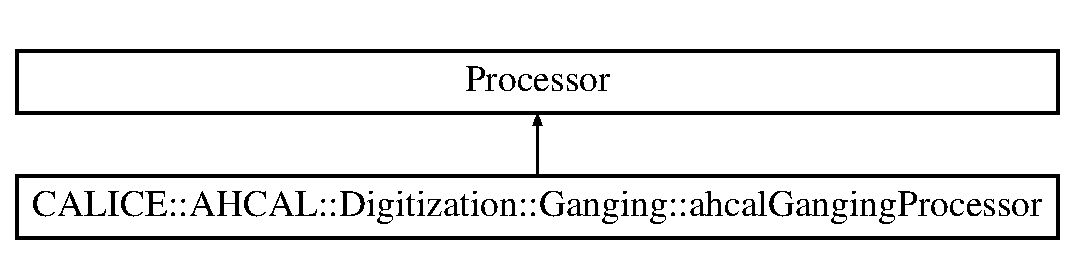
\includegraphics[height=2.000000cm]{classCALICE_1_1AHCAL_1_1Digitization_1_1Ganging_1_1ahcalGangingProcessor}
\end{center}
\end{figure}
\subsection*{Public Member Functions}
\begin{DoxyCompactItemize}
\item 
marlin\-::\-Processor $\ast$ {\bfseries new\-Processor} ()\label{classCALICE_1_1AHCAL_1_1Digitization_1_1Ganging_1_1ahcalGangingProcessor_a9a66e176471d6bab6a78a591c7a8fe14}

\item 
void {\bf init} ()
\begin{DoxyCompactList}\small\item\em Initiliases the ganging chain of responsibilty for fine and coarse modules. \end{DoxyCompactList}\item 
void {\bf process\-Event} (lcio\-::\-L\-C\-Event $\ast$evt)\label{classCALICE_1_1AHCAL_1_1Digitization_1_1Ganging_1_1ahcalGangingProcessor_a4472b19f4354ed820e033c649a6464dd}

\begin{DoxyCompactList}\small\item\em Called every event. \end{DoxyCompactList}\item 
float {\bf energy\-Sum} (std\-::vector$<$ Sim\-Calorimeter\-Hit $\ast$ $>$ vec\-Sim\-Hits)\label{classCALICE_1_1AHCAL_1_1Digitization_1_1Ganging_1_1ahcalGangingProcessor_ad7057224da280aae5d6dd0b1b6987f5d}

\begin{DoxyCompactList}\small\item\em Helper function to add up all Sim\-Calorimeter\-Hit energies. \end{DoxyCompactList}\item 
void {\bf create\-Output\-Collections} (lcio\-::\-L\-C\-Event $\ast$evt)\label{classCALICE_1_1AHCAL_1_1Digitization_1_1Ganging_1_1ahcalGangingProcessor_a97a288c25d78ca34a840537937c6e650}

\begin{DoxyCompactList}\small\item\em Creates the ganged collection. \end{DoxyCompactList}\item 
void {\bf tidy\-Up} ()\label{classCALICE_1_1AHCAL_1_1Digitization_1_1Ganging_1_1ahcalGangingProcessor_ae693cebeaff120fdc170c1470efd4f88}

\begin{DoxyCompactList}\small\item\em Resets everything which is event specific. \end{DoxyCompactList}\item 
void {\bfseries end} ()\label{classCALICE_1_1AHCAL_1_1Digitization_1_1Ganging_1_1ahcalGangingProcessor_ac8591372ea5a0fde5b77d10cc3cb1187}

\end{DoxyCompactItemize}
\subsection*{Private Attributes}
\begin{DoxyCompactItemize}
\item 
std\-::string {\bf \-\_\-input\-Collection\-Name}\label{classCALICE_1_1AHCAL_1_1Digitization_1_1Ganging_1_1ahcalGangingProcessor_a86280fa3badb720de25a0580e5d57223}

\begin{DoxyCompactList}\small\item\em The name of the incoming collection. \end{DoxyCompactList}\item 
std\-::string {\bf \-\_\-output\-Collection\-Name}\label{classCALICE_1_1AHCAL_1_1Digitization_1_1Ganging_1_1ahcalGangingProcessor_a3bb50975778976e74b076ac14059fd81}

\begin{DoxyCompactList}\small\item\em The name of the outgoing collection. \end{DoxyCompactList}\item 
float {\bfseries \-\_\-tile\-Border\-Attenuation\-Factor}\label{classCALICE_1_1AHCAL_1_1Digitization_1_1Ganging_1_1ahcalGangingProcessor_a3b6ac87efbe5f79354ecf9bb86f6b641}

\item 
{\bf Contribution\-Map} {\bf \-\_\-contribution\-Map}
\begin{DoxyCompactList}\small\item\em Instance which holds the gather Sim\-Calorimeter\-Hits. \end{DoxyCompactList}\item 
std\-::vector$<$ {\bf Ganger} $\ast$ $>$ {\bf \-\_\-gangers\-For\-Fine\-Modules}
\begin{DoxyCompactList}\small\item\em All gangers needed for a fine module. \end{DoxyCompactList}\item 
std\-::vector$<$ {\bf Ganger} $\ast$ $>$ {\bf \-\_\-gangers\-For\-Coarse\-Modules}
\begin{DoxyCompactList}\small\item\em All gangers needed for a coarse module. \end{DoxyCompactList}\item 
std\-::map$<$ int, Module\-Type $>$ {\bf \-\_\-module\-Type\-Order}
\begin{DoxyCompactList}\small\item\em Layer to module type map. \end{DoxyCompactList}\end{DoxyCompactItemize}


\subsection{Detailed Description}
The processor performing the ganging. 

Definition at line 75 of file ahcal\-Ganging\-Processor.\-hh.



\subsection{Member Function Documentation}
\index{C\-A\-L\-I\-C\-E\-::\-A\-H\-C\-A\-L\-::\-Digitization\-::\-Ganging\-::ahcal\-Ganging\-Processor@{C\-A\-L\-I\-C\-E\-::\-A\-H\-C\-A\-L\-::\-Digitization\-::\-Ganging\-::ahcal\-Ganging\-Processor}!init@{init}}
\index{init@{init}!CALICE::AHCAL::Digitization::Ganging::ahcalGangingProcessor@{C\-A\-L\-I\-C\-E\-::\-A\-H\-C\-A\-L\-::\-Digitization\-::\-Ganging\-::ahcal\-Ganging\-Processor}}
\subsubsection[{init}]{\setlength{\rightskip}{0pt plus 5cm}void ahcal\-Ganging\-Processor\-::init (
\begin{DoxyParamCaption}
{}
\end{DoxyParamCaption}
)}\label{classCALICE_1_1AHCAL_1_1Digitization_1_1Ganging_1_1ahcalGangingProcessor_af1f1ff625562d20de4107f25a9998394}


Initiliases the ganging chain of responsibilty for fine and coarse modules. 

Defines location of module types. 

Definition at line 166 of file ahcal\-Ganging\-Processor.\-cc.



\subsection{Field Documentation}
\index{C\-A\-L\-I\-C\-E\-::\-A\-H\-C\-A\-L\-::\-Digitization\-::\-Ganging\-::ahcal\-Ganging\-Processor@{C\-A\-L\-I\-C\-E\-::\-A\-H\-C\-A\-L\-::\-Digitization\-::\-Ganging\-::ahcal\-Ganging\-Processor}!\-\_\-contribution\-Map@{\-\_\-contribution\-Map}}
\index{\-\_\-contribution\-Map@{\-\_\-contribution\-Map}!CALICE::AHCAL::Digitization::Ganging::ahcalGangingProcessor@{C\-A\-L\-I\-C\-E\-::\-A\-H\-C\-A\-L\-::\-Digitization\-::\-Ganging\-::ahcal\-Ganging\-Processor}}
\subsubsection[{\-\_\-contribution\-Map}]{\setlength{\rightskip}{0pt plus 5cm}{\bf Contribution\-Map} C\-A\-L\-I\-C\-E\-::\-A\-H\-C\-A\-L\-::\-Digitization\-::\-Ganging\-::ahcal\-Ganging\-Processor\-::\-\_\-contribution\-Map\hspace{0.3cm}{\ttfamily [private]}}\label{classCALICE_1_1AHCAL_1_1Digitization_1_1Ganging_1_1ahcalGangingProcessor_a8440464f02c34f8267bc3fffc23e5f5f}


Instance which holds the gather Sim\-Calorimeter\-Hits. 

The outcome of the ganging is here. 

Definition at line 125 of file ahcal\-Ganging\-Processor.\-hh.

\index{C\-A\-L\-I\-C\-E\-::\-A\-H\-C\-A\-L\-::\-Digitization\-::\-Ganging\-::ahcal\-Ganging\-Processor@{C\-A\-L\-I\-C\-E\-::\-A\-H\-C\-A\-L\-::\-Digitization\-::\-Ganging\-::ahcal\-Ganging\-Processor}!\-\_\-gangers\-For\-Coarse\-Modules@{\-\_\-gangers\-For\-Coarse\-Modules}}
\index{\-\_\-gangers\-For\-Coarse\-Modules@{\-\_\-gangers\-For\-Coarse\-Modules}!CALICE::AHCAL::Digitization::Ganging::ahcalGangingProcessor@{C\-A\-L\-I\-C\-E\-::\-A\-H\-C\-A\-L\-::\-Digitization\-::\-Ganging\-::ahcal\-Ganging\-Processor}}
\subsubsection[{\-\_\-gangers\-For\-Coarse\-Modules}]{\setlength{\rightskip}{0pt plus 5cm}std\-::vector$<${\bf Ganger}$\ast$$>$ C\-A\-L\-I\-C\-E\-::\-A\-H\-C\-A\-L\-::\-Digitization\-::\-Ganging\-::ahcal\-Ganging\-Processor\-::\-\_\-gangers\-For\-Coarse\-Modules\hspace{0.3cm}{\ttfamily [private]}}\label{classCALICE_1_1AHCAL_1_1Digitization_1_1Ganging_1_1ahcalGangingProcessor_a3136b9597513288f99e8f4e5599da935}


All gangers needed for a coarse module. 

Filled in \doxyref{init()}{p.}{classCALICE_1_1AHCAL_1_1Digitization_1_1Ganging_1_1ahcalGangingProcessor_af1f1ff625562d20de4107f25a9998394}. 

Definition at line 133 of file ahcal\-Ganging\-Processor.\-hh.

\index{C\-A\-L\-I\-C\-E\-::\-A\-H\-C\-A\-L\-::\-Digitization\-::\-Ganging\-::ahcal\-Ganging\-Processor@{C\-A\-L\-I\-C\-E\-::\-A\-H\-C\-A\-L\-::\-Digitization\-::\-Ganging\-::ahcal\-Ganging\-Processor}!\-\_\-gangers\-For\-Fine\-Modules@{\-\_\-gangers\-For\-Fine\-Modules}}
\index{\-\_\-gangers\-For\-Fine\-Modules@{\-\_\-gangers\-For\-Fine\-Modules}!CALICE::AHCAL::Digitization::Ganging::ahcalGangingProcessor@{C\-A\-L\-I\-C\-E\-::\-A\-H\-C\-A\-L\-::\-Digitization\-::\-Ganging\-::ahcal\-Ganging\-Processor}}
\subsubsection[{\-\_\-gangers\-For\-Fine\-Modules}]{\setlength{\rightskip}{0pt plus 5cm}std\-::vector$<${\bf Ganger}$\ast$$>$ C\-A\-L\-I\-C\-E\-::\-A\-H\-C\-A\-L\-::\-Digitization\-::\-Ganging\-::ahcal\-Ganging\-Processor\-::\-\_\-gangers\-For\-Fine\-Modules\hspace{0.3cm}{\ttfamily [private]}}\label{classCALICE_1_1AHCAL_1_1Digitization_1_1Ganging_1_1ahcalGangingProcessor_aec06e26e5edfbccd58b555e87ea08f27}


All gangers needed for a fine module. 

Filled in \doxyref{init()}{p.}{classCALICE_1_1AHCAL_1_1Digitization_1_1Ganging_1_1ahcalGangingProcessor_af1f1ff625562d20de4107f25a9998394}. 

Definition at line 129 of file ahcal\-Ganging\-Processor.\-hh.

\index{C\-A\-L\-I\-C\-E\-::\-A\-H\-C\-A\-L\-::\-Digitization\-::\-Ganging\-::ahcal\-Ganging\-Processor@{C\-A\-L\-I\-C\-E\-::\-A\-H\-C\-A\-L\-::\-Digitization\-::\-Ganging\-::ahcal\-Ganging\-Processor}!\-\_\-module\-Type\-Order@{\-\_\-module\-Type\-Order}}
\index{\-\_\-module\-Type\-Order@{\-\_\-module\-Type\-Order}!CALICE::AHCAL::Digitization::Ganging::ahcalGangingProcessor@{C\-A\-L\-I\-C\-E\-::\-A\-H\-C\-A\-L\-::\-Digitization\-::\-Ganging\-::ahcal\-Ganging\-Processor}}
\subsubsection[{\-\_\-module\-Type\-Order}]{\setlength{\rightskip}{0pt plus 5cm}std\-::map$<$int,Module\-Type$>$ C\-A\-L\-I\-C\-E\-::\-A\-H\-C\-A\-L\-::\-Digitization\-::\-Ganging\-::ahcal\-Ganging\-Processor\-::\-\_\-module\-Type\-Order\hspace{0.3cm}{\ttfamily [private]}}\label{classCALICE_1_1AHCAL_1_1Digitization_1_1Ganging_1_1ahcalGangingProcessor_a1cb7ea3c7daaca045c4d5147eaa077da}


Layer to module type map. 

Filled in \doxyref{init()}{p.}{classCALICE_1_1AHCAL_1_1Digitization_1_1Ganging_1_1ahcalGangingProcessor_af1f1ff625562d20de4107f25a9998394}. 

Definition at line 137 of file ahcal\-Ganging\-Processor.\-hh.



The documentation for this class was generated from the following files\-:\begin{DoxyCompactItemize}
\item 
ahcal\-Ganging\-Processor.\-hh\item 
ahcal\-Ganging\-Processor.\-cc\end{DoxyCompactItemize}

\section{C\-A\-L\-I\-C\-E\-:\-:Ahc\-Digitisation\-Processor Class Reference}
\label{classCALICE_1_1AhcDigitisationProcessor}\index{C\-A\-L\-I\-C\-E\-::\-Ahc\-Digitisation\-Processor@{C\-A\-L\-I\-C\-E\-::\-Ahc\-Digitisation\-Processor}}


Class for doing the \doxyref{A\-H\-C\-A\-L}{p.}{namespaceCALICE_1_1AHCAL} digitisation.  




{\ttfamily \#include $<$Ahc\-Digitisation\-Processor.\-hh$>$}

Inheritance diagram for C\-A\-L\-I\-C\-E\-:\-:Ahc\-Digitisation\-Processor\-:\begin{figure}[H]
\begin{center}
\leavevmode
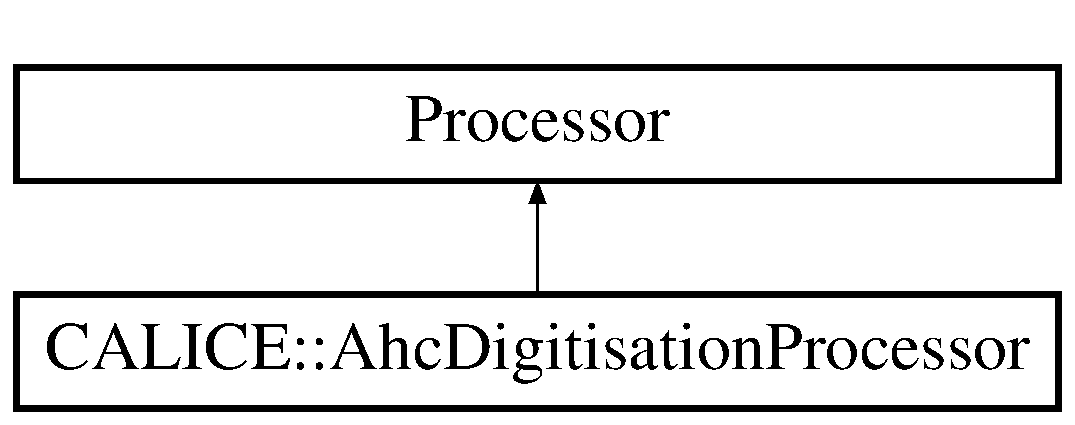
\includegraphics[height=2.000000cm]{classCALICE_1_1AhcDigitisationProcessor}
\end{center}
\end{figure}
\subsection*{Public Member Functions}
\begin{DoxyCompactItemize}
\item 
{\bf Ahc\-Digitisation\-Processor} (const std\-::string processor\-Name=\char`\"{}Ahc\-Digitisation\-Processor\char`\"{})\label{classCALICE_1_1AhcDigitisationProcessor_ac6d5d7399a3b6a27089e9dde461b2d5a}

\begin{DoxyCompactList}\small\item\em Constructor. \end{DoxyCompactList}\item 
virtual {\bf $\sim$\-Ahc\-Digitisation\-Processor} ()\label{classCALICE_1_1AhcDigitisationProcessor_a199927dbc65fcd321b131917dcfe260e}

\begin{DoxyCompactList}\small\item\em Destructor. \end{DoxyCompactList}\item 
{\bf Ahc\-Digitisation\-Processor} $\ast$ {\bfseries new\-Processor} ()\label{classCALICE_1_1AhcDigitisationProcessor_af899a14b8116b8784e83f6588e312665}

\item 
virtual void {\bf init} ()\label{classCALICE_1_1AhcDigitisationProcessor_a50f3bf333cdb63d658983d72b359ba83}

\begin{DoxyCompactList}\small\item\em Initialise. \end{DoxyCompactList}\item 
virtual void {\bf process\-Event} (lcio\-::\-L\-C\-Event $\ast$)\label{classCALICE_1_1AhcDigitisationProcessor_a0ebdc81c82c6c1a2b04ce517748d0b08}

\begin{DoxyCompactList}\small\item\em Process event (the working horse) \end{DoxyCompactList}\item 
virtual void {\bf end} ()\label{classCALICE_1_1AhcDigitisationProcessor_a36b498cc10f444ec3dc618481f52ab5b}

\begin{DoxyCompactList}\small\item\em End of processing. \end{DoxyCompactList}\end{DoxyCompactItemize}
\subsection*{Protected Member Functions}
\begin{DoxyCompactItemize}
\item 
void {\bf fill\-Ganged\-Container} (L\-C\-Collection $\ast$input\-Col)
\begin{DoxyCompactList}\small\item\em Fill a mapped container with the ganged \doxyref{A\-H\-C\-A\-L}{p.}{namespaceCALICE_1_1AHCAL} cells. \end{DoxyCompactList}\item 
void {\bf simulate\-Optical\-Cross\-Talk} ()
\begin{DoxyCompactList}\small\item\em Simulate the optical cross-\/talk (i.\-e. \end{DoxyCompactList}\item 
void {\bf simulate\-Si\-P\-M\-Behaviour} ()\label{classCALICE_1_1AhcDigitisationProcessor_aa63b9bab2faf9b7dd8b46d131e60a91f}

\begin{DoxyCompactList}\small\item\em Simulate the Si\-P\-M binomial behaviour. \end{DoxyCompactList}\item 
void {\bf add\-Noise} (L\-C\-Collection $\ast$noise\-Col)
\begin{DoxyCompactList}\small\item\em Add noise events from data. \end{DoxyCompactList}\item 
void {\bf create\-Output\-Collection} (L\-C\-Event $\ast$evt)
\begin{DoxyCompactList}\small\item\em Create output collection of digitised \doxyref{A\-H\-C\-A\-L}{p.}{namespaceCALICE_1_1AHCAL} hits. \end{DoxyCompactList}\item 
void {\bf write\-Collection\-For\-Debug} (L\-C\-Event $\ast$evt, const std\-::string col\-Name)
\begin{DoxyCompactList}\small\item\em Write collections after each step in digitisation, for debugging purposes. \end{DoxyCompactList}\end{DoxyCompactItemize}
\subsection*{Private Attributes}
\begin{DoxyCompactItemize}
\item 
std\-::string {\bf \-\_\-input\-Col\-Name}\label{classCALICE_1_1AhcDigitisationProcessor_a72bda23d0bbb7f6d2a18e204b9a36463}

\begin{DoxyCompactList}\small\item\em name of the input collection \end{DoxyCompactList}\item 
std\-::string {\bf \-\_\-output\-Col\-Name}\label{classCALICE_1_1AhcDigitisationProcessor_ad3fe495aecfc6b5ad5d705bfede2edc5}

\begin{DoxyCompactList}\small\item\em name of the output collection \end{DoxyCompactList}\item 
std\-::string {\bf \-\_\-noise\-Col\-Name}\label{classCALICE_1_1AhcDigitisationProcessor_afcf557188248cfb03958d6a0ffbff1fd}

\begin{DoxyCompactList}\small\item\em name of the \doxyref{A\-H\-C\-A\-L}{p.}{namespaceCALICE_1_1AHCAL} noise collection \end{DoxyCompactList}\item 
std\-::string {\bf \-\_\-mapping\-Processor\-Name}\label{classCALICE_1_1AhcDigitisationProcessor_acaf77fc25248da21eb986295916d4bc3}

\begin{DoxyCompactList}\small\item\em name of the mapping processor name \end{DoxyCompactList}\item 
std\-::string {\bf \-\_\-cell\-Neighbours\-Processor\-Name}\label{classCALICE_1_1AhcDigitisationProcessor_ac7a70be0c607cf7f42a49c21682c35e2}

\begin{DoxyCompactList}\small\item\em name of the processor which provides the cells neighbours \end{DoxyCompactList}\item 
std\-::string {\bf \-\_\-cell\-Description\-Processor\-Name}\label{classCALICE_1_1AhcDigitisationProcessor_adb82414851fca1623d2819bd063450f9}

\begin{DoxyCompactList}\small\item\em name of the processor which provides the cells description \end{DoxyCompactList}\item 
std\-::string {\bf \-\_\-calib\-Processor\-Name}\label{classCALICE_1_1AhcDigitisationProcessor_a45bc5cc91c44e99857db273a32d4c27b}

\begin{DoxyCompactList}\small\item\em name of the processor which provides the Si\-P\-M calibrations \end{DoxyCompactList}\item 
std\-::string {\bf \-\_\-temperature\-Processor\-Name}\label{classCALICE_1_1AhcDigitisationProcessor_afd9832a3066c9a63d566214b7c3a3270}

\begin{DoxyCompactList}\small\item\em name of the processor which provides the cell temperature \end{DoxyCompactList}\item 
std\-::string {\bf \-\_\-sim\-Rec\-Relation\-Col\-Name}\label{classCALICE_1_1AhcDigitisationProcessor_a38db427f6421c7645321343a36ed2a31}

\begin{DoxyCompactList}\small\item\em name of the relation between Mokka Sim\-Calorimeter\-Hits and reconstructed Calorimeter\-Hits \end{DoxyCompactList}\item 
Mapped\-Container\\*
$<$ C\-A\-L\-I\-C\-E\-::\-Cell\-Description $>$ $\ast$ {\bf \-\_\-cell\-Descriptions}\label{classCALICE_1_1AhcDigitisationProcessor_a7e32e9a109e5cb073c42f47007b7c053}

\begin{DoxyCompactList}\small\item\em mapped container of cells description \end{DoxyCompactList}\item 
Mapped\-Container\\*
$<$ C\-A\-L\-I\-C\-E\-::\-Cell\-Neighbours $>$ $\ast$ {\bf \-\_\-cell\-Neighbours}\label{classCALICE_1_1AhcDigitisationProcessor_ab93720861f27ca6f83817c0d3f211445}

\begin{DoxyCompactList}\small\item\em mapped container of cells neighbours \end{DoxyCompactList}\item 
Mapped\-Container\\*
$<$ Si\-P\-M\-Calibrations $>$ $\ast$ {\bf \-\_\-calib\-Container}\label{classCALICE_1_1AhcDigitisationProcessor_ab7f981a098e38f9b59c88f0ba33397c9}

\begin{DoxyCompactList}\small\item\em mapped container of Si\-P\-M calibrations \end{DoxyCompactList}\item 
Mapped\-Container\\*
$<$ Calorimeter\-Hit\-Impl $>$ $\ast$ {\bf \-\_\-ganged\-Container}\label{classCALICE_1_1AhcDigitisationProcessor_a3b76cd6f9f5aba3fbe3f60ddb6dc1bb6}

\begin{DoxyCompactList}\small\item\em mapped container of ganged \doxyref{A\-H\-C\-A\-L}{p.}{namespaceCALICE_1_1AHCAL} cells \end{DoxyCompactList}\item 
float {\bf \-\_\-mip\-Per\-Ge\-V\-Factor}\label{classCALICE_1_1AhcDigitisationProcessor_a6ef245fe28f55767632ff05e77d9a829}

\begin{DoxyCompactList}\small\item\em the M\-I\-P to Ge\-V factor (determined with muon events in Monte Carlo) \end{DoxyCompactList}\item 
float {\bf \-\_\-light\-Leakage}\label{classCALICE_1_1AhcDigitisationProcessor_a1e9e0d0528dc47d7c9c19ac6586a71ea}

\begin{DoxyCompactList}\small\item\em light leakage factor \end{DoxyCompactList}\item 
bool {\bf \-\_\-create\-Sim\-Rec\-Relation}\label{classCALICE_1_1AhcDigitisationProcessor_a6c916929baa666c12298e317817084e4}

\begin{DoxyCompactList}\small\item\em flag to disable/enable the creation of an L\-C\-Relation between the Mokka Sim\-Calorimeter\-Hits and the reconstructed Calorimeter\-Hits \end{DoxyCompactList}\item 
bool {\bf \-\_\-do\-Binomial\-Smearing}\label{classCALICE_1_1AhcDigitisationProcessor_a30ba04dfeb3747c4f71f958f245a13bc}

\begin{DoxyCompactList}\small\item\em flag to disable/enable binomial smearing \end{DoxyCompactList}\item 
bool {\bf \-\_\-do\-Saturation}\label{classCALICE_1_1AhcDigitisationProcessor_aa916607376cccbd85fbfb26eb13c3bb7}

\begin{DoxyCompactList}\small\item\em flag to disable/enable Si\-P\-M saturation behaver to ture M\-C \end{DoxyCompactList}\item 
bool {\bf \-\_\-do\-Optical\-Cross\-Talk}\label{classCALICE_1_1AhcDigitisationProcessor_a075b820df994ae1c8821ed645bb66e75}

\begin{DoxyCompactList}\small\item\em flag to disable/enable optical cross talk among neighbour tiles \end{DoxyCompactList}\item 
bool {\bf \-\_\-do\-Add\-Noise}\label{classCALICE_1_1AhcDigitisationProcessor_a26d22b77b485d343f29f3a98cc9f1534}

\begin{DoxyCompactList}\small\item\em flag to disable/enable adding detector noise \end{DoxyCompactList}\item 
bool {\bf \-\_\-do\-Write\-Collection\-For\-Debug}\label{classCALICE_1_1AhcDigitisationProcessor_afe79a2e72054025e9c239da37fe53ea4}

\begin{DoxyCompactList}\small\item\em flag to disable/enable the writing of collections after each step in digitisation, for debugging \end{DoxyCompactList}\item 
bool {\bfseries \-\_\-do\-Mip\-Temp\-Corr}\label{classCALICE_1_1AhcDigitisationProcessor_afa09643e559a7a297525ad6541ec355c}

\item 
bool {\bfseries \-\_\-do\-Gain\-Temp\-Corr}\label{classCALICE_1_1AhcDigitisationProcessor_a61e0a30e65097cb54e665eadfa03c1e7}

\item 
const Mapper $\ast$ {\bf \-\_\-mapper}\label{classCALICE_1_1AhcDigitisationProcessor_acdb431b7145ac67ce614b16515f68962}

\begin{DoxyCompactList}\small\item\em pointer to the used mapped \end{DoxyCompactList}\item 
unsigned int {\bf \-\_\-mapper\-Version}\label{classCALICE_1_1AhcDigitisationProcessor_a601169fba8b997ddfe9c0fbc6350ceaf}

\begin{DoxyCompactList}\small\item\em mapper version \end{DoxyCompactList}\item 
bool {\bfseries \-\_\-correct\-Default\-Gain\-To\-L\-Y}\label{classCALICE_1_1AhcDigitisationProcessor_a61b4bcfff3e4655a52f06b959cf475f7}

\item 
float {\bfseries \-\_\-fixed\-L\-Y}\label{classCALICE_1_1AhcDigitisationProcessor_ae4400a9e07b000f1f68336d17b704de9}

\item 
T\-Random3 $\ast$ {\bf \-\_\-random\-Generator}\label{classCALICE_1_1AhcDigitisationProcessor_a768c421df0cce682c8f145a8b5ca6659}

\begin{DoxyCompactList}\small\item\em pointer to R\-O\-O\-Ts random generator for pixel statistics \end{DoxyCompactList}\item 
int {\bf \-\_\-random\-Seed}
\begin{DoxyCompactList}\small\item\em random seed for the random generator. \end{DoxyCompactList}\item 
std\-::string {\bf \-\_\-mokka\-Encoding\-String}\label{classCALICE_1_1AhcDigitisationProcessor_a831dc9819703c4ab138e232856b4d06c}

\begin{DoxyCompactList}\small\item\em the Mokka encoding string \end{DoxyCompactList}\end{DoxyCompactItemize}
\subsection*{Static Private Attributes}
\begin{DoxyCompactItemize}
\item 
static const unsigned int {\bf M\-A\-X\-A\-D\-C} = 31768\label{classCALICE_1_1AhcDigitisationProcessor_a34e064b2439ad95265f45971621dd75a}

\begin{DoxyCompactList}\small\item\em conservative maximum number of A\-D\-C channels the hardware provides, 32768 -\/ 1000 (average pedestal) \end{DoxyCompactList}\end{DoxyCompactItemize}


\subsection{Detailed Description}
Class for doing the \doxyref{A\-H\-C\-A\-L}{p.}{namespaceCALICE_1_1AHCAL} digitisation. 

For more details, have a look here\-: {\tt http\-://www-\/flc.\-desy.\-de/hcal/documents/2008/diplom.\-2008.\-richter.\-pdf}

\begin{DoxyAuthor}{Author}
{\tt lucaci@mail.\-desy.\-de} 
\end{DoxyAuthor}
\begin{DoxyVersion}{Version}
1.\-0 
\end{DoxyVersion}
\begin{DoxyDate}{Date}
April 2010 
\end{DoxyDate}


Definition at line 30 of file Ahc\-Digitisation\-Processor.\-hh.



\subsection{Member Function Documentation}
\index{C\-A\-L\-I\-C\-E\-::\-Ahc\-Digitisation\-Processor@{C\-A\-L\-I\-C\-E\-::\-Ahc\-Digitisation\-Processor}!add\-Noise@{add\-Noise}}
\index{add\-Noise@{add\-Noise}!CALICE::AhcDigitisationProcessor@{C\-A\-L\-I\-C\-E\-::\-Ahc\-Digitisation\-Processor}}
\subsubsection[{add\-Noise}]{\setlength{\rightskip}{0pt plus 5cm}void C\-A\-L\-I\-C\-E\-::\-Ahc\-Digitisation\-Processor\-::add\-Noise (
\begin{DoxyParamCaption}
\item[{L\-C\-Collection $\ast$}]{noise\-Col}
\end{DoxyParamCaption}
)\hspace{0.3cm}{\ttfamily [protected]}}\label{classCALICE_1_1AhcDigitisationProcessor_a2b8791a0e9f1abb9307ab4595fdd57ca}


Add noise events from data. 


\begin{DoxyParams}{Parameters}
{\em noise\-Col} & the noise collection \\
\hline
\end{DoxyParams}


Definition at line 676 of file Ahc\-Digitisation\-Processor.\-cc.



References \-\_\-do\-Add\-Noise, \-\_\-do\-Saturation, \-\_\-ganged\-Container, \-\_\-mokka\-Encoding\-String, and M\-A\-X\-A\-D\-C.



Referenced by process\-Event().

\index{C\-A\-L\-I\-C\-E\-::\-Ahc\-Digitisation\-Processor@{C\-A\-L\-I\-C\-E\-::\-Ahc\-Digitisation\-Processor}!create\-Output\-Collection@{create\-Output\-Collection}}
\index{create\-Output\-Collection@{create\-Output\-Collection}!CALICE::AhcDigitisationProcessor@{C\-A\-L\-I\-C\-E\-::\-Ahc\-Digitisation\-Processor}}
\subsubsection[{create\-Output\-Collection}]{\setlength{\rightskip}{0pt plus 5cm}void C\-A\-L\-I\-C\-E\-::\-Ahc\-Digitisation\-Processor\-::create\-Output\-Collection (
\begin{DoxyParamCaption}
\item[{L\-C\-Event $\ast$}]{evt}
\end{DoxyParamCaption}
)\hspace{0.3cm}{\ttfamily [protected]}}\label{classCALICE_1_1AhcDigitisationProcessor_a2a61ddaf010ad7cba91246bbcb817063}


Create output collection of digitised \doxyref{A\-H\-C\-A\-L}{p.}{namespaceCALICE_1_1AHCAL} hits. 


\begin{DoxyParams}{Parameters}
{\em evt} & L\-C\-Event to which the collection will be added \\
\hline
\end{DoxyParams}


Definition at line 744 of file Ahc\-Digitisation\-Processor.\-cc.



References \-\_\-ganged\-Container, \-\_\-mokka\-Encoding\-String, and \-\_\-output\-Col\-Name.



Referenced by process\-Event().

\index{C\-A\-L\-I\-C\-E\-::\-Ahc\-Digitisation\-Processor@{C\-A\-L\-I\-C\-E\-::\-Ahc\-Digitisation\-Processor}!fill\-Ganged\-Container@{fill\-Ganged\-Container}}
\index{fill\-Ganged\-Container@{fill\-Ganged\-Container}!CALICE::AhcDigitisationProcessor@{C\-A\-L\-I\-C\-E\-::\-Ahc\-Digitisation\-Processor}}
\subsubsection[{fill\-Ganged\-Container}]{\setlength{\rightskip}{0pt plus 5cm}void C\-A\-L\-I\-C\-E\-::\-Ahc\-Digitisation\-Processor\-::fill\-Ganged\-Container (
\begin{DoxyParamCaption}
\item[{L\-C\-Collection $\ast$}]{input\-Col}
\end{DoxyParamCaption}
)\hspace{0.3cm}{\ttfamily [protected]}}\label{classCALICE_1_1AhcDigitisationProcessor_a1f11528ab52b6152a1526937e24ab2b3}


Fill a mapped container with the ganged \doxyref{A\-H\-C\-A\-L}{p.}{namespaceCALICE_1_1AHCAL} cells. 

By default, Mokka creates 10x10 mm$^\wedge$2 cells. During ganging (i.\-e. grouping), the Mokka cells are grouped into 30x30 mm$^\wedge$2, 60x60 mm$^\wedge$2 and 120x120 mm$^\wedge$2 cells 
\begin{DoxyParams}{Parameters}
{\em input\-Col} & the input collection, with the \doxyref{A\-H\-C\-A\-L}{p.}{namespaceCALICE_1_1AHCAL} Mokka hits \\
\hline
\end{DoxyParams}


Definition at line 290 of file Ahc\-Digitisation\-Processor.\-cc.



References \-\_\-ganged\-Container, \-\_\-mapper, \-\_\-mip\-Per\-Ge\-V\-Factor, and \-\_\-mokka\-Encoding\-String.



Referenced by process\-Event().

\index{C\-A\-L\-I\-C\-E\-::\-Ahc\-Digitisation\-Processor@{C\-A\-L\-I\-C\-E\-::\-Ahc\-Digitisation\-Processor}!simulate\-Optical\-Cross\-Talk@{simulate\-Optical\-Cross\-Talk}}
\index{simulate\-Optical\-Cross\-Talk@{simulate\-Optical\-Cross\-Talk}!CALICE::AhcDigitisationProcessor@{C\-A\-L\-I\-C\-E\-::\-Ahc\-Digitisation\-Processor}}
\subsubsection[{simulate\-Optical\-Cross\-Talk}]{\setlength{\rightskip}{0pt plus 5cm}void C\-A\-L\-I\-C\-E\-::\-Ahc\-Digitisation\-Processor\-::simulate\-Optical\-Cross\-Talk (
\begin{DoxyParamCaption}
{}
\end{DoxyParamCaption}
)\hspace{0.3cm}{\ttfamily [protected]}}\label{classCALICE_1_1AhcDigitisationProcessor_abb6aeaac9f722631e32656a59a32b4ab}


Simulate the optical cross-\/talk (i.\-e. 

light leakage) between the tiles 

Definition at line 329 of file Ahc\-Digitisation\-Processor.\-cc.



References \-\_\-cell\-Descriptions, \-\_\-cell\-Neighbours, \-\_\-cell\-Neighbours\-Processor\-Name, \-\_\-ganged\-Container, \-\_\-light\-Leakage, and \-\_\-mokka\-Encoding\-String.



Referenced by process\-Event().

\index{C\-A\-L\-I\-C\-E\-::\-Ahc\-Digitisation\-Processor@{C\-A\-L\-I\-C\-E\-::\-Ahc\-Digitisation\-Processor}!write\-Collection\-For\-Debug@{write\-Collection\-For\-Debug}}
\index{write\-Collection\-For\-Debug@{write\-Collection\-For\-Debug}!CALICE::AhcDigitisationProcessor@{C\-A\-L\-I\-C\-E\-::\-Ahc\-Digitisation\-Processor}}
\subsubsection[{write\-Collection\-For\-Debug}]{\setlength{\rightskip}{0pt plus 5cm}void C\-A\-L\-I\-C\-E\-::\-Ahc\-Digitisation\-Processor\-::write\-Collection\-For\-Debug (
\begin{DoxyParamCaption}
\item[{L\-C\-Event $\ast$}]{evt, }
\item[{const std\-::string}]{col\-Name}
\end{DoxyParamCaption}
)\hspace{0.3cm}{\ttfamily [protected]}}\label{classCALICE_1_1AhcDigitisationProcessor_af7f0890bc1d7d7277b364931b83177b5}


Write collections after each step in digitisation, for debugging purposes. 


\begin{DoxyParams}{Parameters}
{\em evt} & L\-C\-Event to which the collection will be added \\
\hline
{\em col\-Name} & name of the collection to be written \\
\hline
\end{DoxyParams}


Definition at line 785 of file Ahc\-Digitisation\-Processor.\-cc.



References \-\_\-ganged\-Container, and \-\_\-mokka\-Encoding\-String.



Referenced by process\-Event().



\subsection{Field Documentation}
\index{C\-A\-L\-I\-C\-E\-::\-Ahc\-Digitisation\-Processor@{C\-A\-L\-I\-C\-E\-::\-Ahc\-Digitisation\-Processor}!\-\_\-random\-Seed@{\-\_\-random\-Seed}}
\index{\-\_\-random\-Seed@{\-\_\-random\-Seed}!CALICE::AhcDigitisationProcessor@{C\-A\-L\-I\-C\-E\-::\-Ahc\-Digitisation\-Processor}}
\subsubsection[{\-\_\-random\-Seed}]{\setlength{\rightskip}{0pt plus 5cm}int C\-A\-L\-I\-C\-E\-::\-Ahc\-Digitisation\-Processor\-::\-\_\-random\-Seed\hspace{0.3cm}{\ttfamily [private]}}\label{classCALICE_1_1AhcDigitisationProcessor_a2d175f5694eef8ad4d7179f26a48958f}


random seed for the random generator. 

Steerable. 

Definition at line 127 of file Ahc\-Digitisation\-Processor.\-hh.



Referenced by Ahc\-Digitisation\-Processor(), and init().



The documentation for this class was generated from the following files\-:\begin{DoxyCompactItemize}
\item 
Ahc\-Digitisation\-Processor.\-hh\item 
Ahc\-Digitisation\-Processor.\-cc\end{DoxyCompactItemize}

\section{C\-A\-L\-I\-C\-E\-:\-:Ahc\-Ganging\-Processor Class Reference}
\label{classCALICE_1_1AhcGangingProcessor}\index{C\-A\-L\-I\-C\-E\-::\-Ahc\-Ganging\-Processor@{C\-A\-L\-I\-C\-E\-::\-Ahc\-Ganging\-Processor}}


Class for doing the A\-H\-Cal ganging.  




{\ttfamily \#include $<$Ahc\-Ganging\-Processor.\-hh$>$}

Inheritance diagram for C\-A\-L\-I\-C\-E\-:\-:Ahc\-Ganging\-Processor\-:\begin{figure}[H]
\begin{center}
\leavevmode
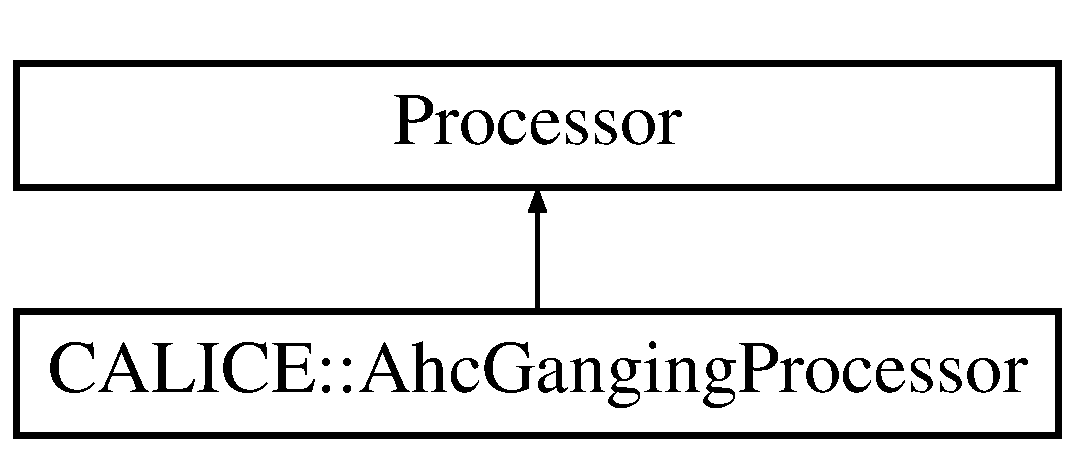
\includegraphics[height=2.000000cm]{classCALICE_1_1AhcGangingProcessor}
\end{center}
\end{figure}
\subsection*{Public Member Functions}
\begin{DoxyCompactItemize}
\item 
{\bf Ahc\-Ganging\-Processor} (const std\-::string processor\-Name=\char`\"{}Ahc\-Ganging\-Processor\char`\"{})\label{classCALICE_1_1AhcGangingProcessor_ac8b6e29deceb4b308b60faa647ccc7e1}

\begin{DoxyCompactList}\small\item\em Constructor. \end{DoxyCompactList}\item 
virtual {\bf $\sim$\-Ahc\-Ganging\-Processor} ()\label{classCALICE_1_1AhcGangingProcessor_a7db28e81275a852ddf7cf10adc78551e}

\begin{DoxyCompactList}\small\item\em Destructor. \end{DoxyCompactList}\item 
{\bf Ahc\-Ganging\-Processor} $\ast$ {\bfseries new\-Processor} ()\label{classCALICE_1_1AhcGangingProcessor_a8fd201ebf38f37964a48e8a672dd8ca5}

\item 
virtual void {\bf init} ()\label{classCALICE_1_1AhcGangingProcessor_a520226589cd39a8d8a1b2160858710b7}

\begin{DoxyCompactList}\small\item\em Initialise. \end{DoxyCompactList}\item 
virtual void {\bf process\-Event} (lcio\-::\-L\-C\-Event $\ast$)\label{classCALICE_1_1AhcGangingProcessor_aaa02bbdc53f1390652d99b909e909348}

\begin{DoxyCompactList}\small\item\em Process event (the working horse) \end{DoxyCompactList}\item 
virtual void {\bf end} ()\label{classCALICE_1_1AhcGangingProcessor_aaaf48bb9209ff61e09b1522cdce9717a}

\begin{DoxyCompactList}\small\item\em End of processing. \end{DoxyCompactList}\end{DoxyCompactItemize}
\subsection*{Private Attributes}
\begin{DoxyCompactItemize}
\item 
std\-::string {\bf \-\_\-input\-Col\-Name}\label{classCALICE_1_1AhcGangingProcessor_ae262d7ff2edd810ae0cc70ab146d3391}

\begin{DoxyCompactList}\small\item\em name of the input collection \end{DoxyCompactList}\item 
std\-::string {\bf \-\_\-output\-Col\-Name}\label{classCALICE_1_1AhcGangingProcessor_a54dca9b895d4f5c53f4852d3d85b105a}

\begin{DoxyCompactList}\small\item\em name of the output collection \end{DoxyCompactList}\item 
std\-::string {\bf \-\_\-mapping\-Processor\-Name}\label{classCALICE_1_1AhcGangingProcessor_afe6bd13c1a2131da9f7d78cc10e45086}

\begin{DoxyCompactList}\small\item\em name of the mapping processor name \end{DoxyCompactList}\item 
std\-::string {\bf \-\_\-cell\-Neighbours\-Processor\-Name}\label{classCALICE_1_1AhcGangingProcessor_aa2d3fd6847cd991e38298f6fe4646e02}

\begin{DoxyCompactList}\small\item\em name of the processor which provides the cells neighbours \end{DoxyCompactList}\item 
std\-::string {\bf \-\_\-cell\-Description\-Processor\-Name}\label{classCALICE_1_1AhcGangingProcessor_ad267d00752eb45681cdd337a3c27e709}

\begin{DoxyCompactList}\small\item\em name of the processor which provides the cells description \end{DoxyCompactList}\item 
Mapped\-Container\\*
$<$ C\-A\-L\-I\-C\-E\-::\-Cell\-Description $>$ $\ast$ {\bf \-\_\-cell\-Descriptions}\label{classCALICE_1_1AhcGangingProcessor_a78a2caa52dd8f07379cc1149bda1c569}

\begin{DoxyCompactList}\small\item\em mapped container of cells description \end{DoxyCompactList}\item 
Mapped\-Container\\*
$<$ C\-A\-L\-I\-C\-E\-::\-Cell\-Neighbours $>$ $\ast$ {\bf \-\_\-cell\-Neighbours}\label{classCALICE_1_1AhcGangingProcessor_a5b0f853b298a53cea88ea6120b811afc}

\begin{DoxyCompactList}\small\item\em mapped container of cells neighbours \end{DoxyCompactList}\item 
const Mapper $\ast$ {\bf \-\_\-mapper}\label{classCALICE_1_1AhcGangingProcessor_acc9c305676156405e7d5e70464205d85}

\begin{DoxyCompactList}\small\item\em pointer to the used mapped \end{DoxyCompactList}\end{DoxyCompactItemize}


\subsection{Detailed Description}
Class for doing the A\-H\-Cal ganging. 

For more details, have a look here\-: {\tt http\-://www-\/flc.\-desy.\-de/hcal/documents/2008/diplom.\-2008.\-richter.\-pdf}

\begin{DoxyAuthor}{Author}
{\tt lucaci@mail.\-desy.\-de} 
\end{DoxyAuthor}
\begin{DoxyVersion}{Version}
1.\-0 
\end{DoxyVersion}
\begin{DoxyDate}{Date}
May 2010 
\end{DoxyDate}


Definition at line 25 of file Ahc\-Ganging\-Processor.\-hh.



The documentation for this class was generated from the following files\-:\begin{DoxyCompactItemize}
\item 
Ahc\-Ganging\-Processor.\-hh\item 
Ahc\-Ganging\-Processor.\-cc\end{DoxyCompactItemize}

\section{digisim\-:\-:Analysis Class Reference}
\label{classdigisim_1_1Analysis}\index{digisim\-::\-Analysis@{digisim\-::\-Analysis}}
Inheritance diagram for digisim\-:\-:Analysis\-:\begin{figure}[H]
\begin{center}
\leavevmode
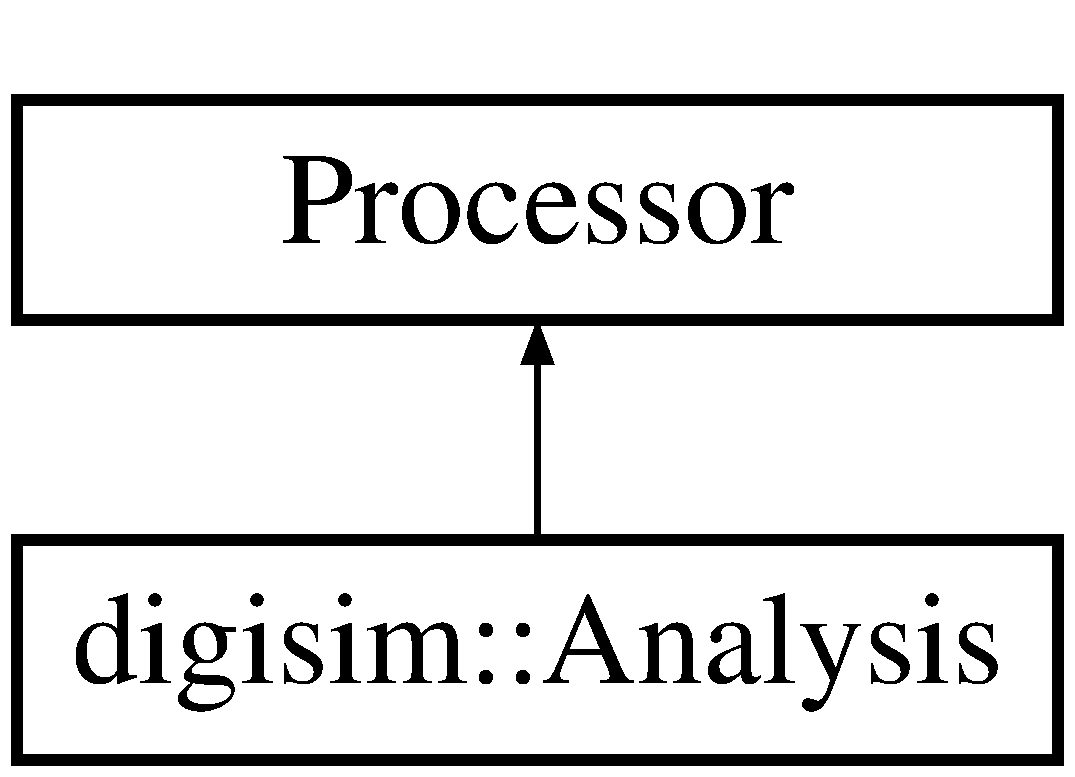
\includegraphics[height=2.000000cm]{classdigisim_1_1Analysis}
\end{center}
\end{figure}
\subsection*{Public Member Functions}
\begin{DoxyCompactItemize}
\item 
virtual Processor $\ast$ {\bfseries new\-Processor} ()\label{classdigisim_1_1Analysis_a7833aa1aec8aba2ff528f318c9f7a21f}

\item 
virtual void {\bf init} ()
\begin{DoxyCompactList}\small\item\em Called at the begin of the job before anything is read. \end{DoxyCompactList}\item 
virtual void {\bf process\-Event} (L\-C\-Event $\ast$evt)
\begin{DoxyCompactList}\small\item\em Called for every run. \end{DoxyCompactList}\item 
virtual void {\bfseries process\-Ecal\-Data} (L\-C\-Event $\ast$evt, std\-::string col\-Name)\label{classdigisim_1_1Analysis_a8d1bb0673ddeb75a6e75f79bbd34bf08}

\item 
virtual void {\bfseries process\-Hcal\-Data} (L\-C\-Event $\ast$evt, std\-::string col\-Name)\label{classdigisim_1_1Analysis_a926b71c47a87e0dab62fba442bc8f470}

\item 
virtual void {\bfseries process\-Tcmt\-Data} (L\-C\-Event $\ast$evt, std\-::string col\-Name)\label{classdigisim_1_1Analysis_ac67d2029aaafe07d629e3544ae87cd77}

\item 
virtual void {\bfseries process\-Hcal\-Raw\-Data} (L\-C\-Event $\ast$evt, std\-::string col\-Name)\label{classdigisim_1_1Analysis_abc397c722130e36df08c04038798024b}

\item 
virtual void {\bf end} ()\label{classdigisim_1_1Analysis_a50de7a9a3fd99be0766ce248fc337d9e}

\begin{DoxyCompactList}\small\item\em Called after data processing for clean up. \end{DoxyCompactList}\end{DoxyCompactItemize}
\subsection*{Protected Attributes}
\begin{DoxyCompactItemize}
\item 
L\-C\-Event $\ast$ {\bfseries \-\_\-evt}\label{classdigisim_1_1Analysis_a2080e48dd7f1a2a4275486263bdaadf6}

\item 
std\-::string {\bfseries \-\_\-tcmt\-Coll\-Name}\label{classdigisim_1_1Analysis_a9613be73c5f30f19f8fa966abe0ad956}

\item 
std\-::string {\bfseries \-\_\-ecal\-Coll\-Name}\label{classdigisim_1_1Analysis_a9dcf5a8273a4c70db4293d5a85625ac3}

\item 
std\-::string {\bfseries \-\_\-hcal\-Coll\-Name}\label{classdigisim_1_1Analysis_aa9e8df324923e3b95a3b666062e712ea}

\item 
int {\bfseries \-\_\-n\-Run}\label{classdigisim_1_1Analysis_a22f4ac6af41dd1ee09f5eadb99c7667a}

\item 
int {\bfseries \-\_\-n\-Evt}\label{classdigisim_1_1Analysis_ad96aa588bfffd028fd3d0570dbf15b14}

\item 
T\-H1\-F $\ast$ {\bfseries \-\_\-h\-Tcmt\-Cell\-Energy}\label{classdigisim_1_1Analysis_adfa670531c288ca2aa896ebc2a696085}

\item 
T\-H1\-F $\ast$ {\bfseries \-\_\-h\-Tcmt\-Cell\-Energy\-M\-I\-P}\label{classdigisim_1_1Analysis_a6f24be97f2b61afd138cc80964acaa10}

\item 
T\-H1\-F $\ast$ {\bfseries \-\_\-h\-Tcmt\-Hits\-Per\-Event}\label{classdigisim_1_1Analysis_af40c47d62f171a8ef64c89ea27adb477}

\item 
T\-Profile $\ast$ {\bfseries \-\_\-h\-Tcmt\-Layer\-Energy}\label{classdigisim_1_1Analysis_aa38b5f4f0176e2f1c587f8d17f20c560}

\item 
T\-Profile $\ast$ {\bfseries \-\_\-h\-Tcmt\-Hits\-Per\-Layer}\label{classdigisim_1_1Analysis_a02a3142dee8ed1f0366d569649b5e9d3}

\item 
T\-H1\-F $\ast$ {\bfseries \-\_\-h\-Ecal\-Cell\-Energy}\label{classdigisim_1_1Analysis_af4dc9cf9e10e1a754f44c2b9171499e2}

\item 
T\-H1\-F $\ast$ {\bfseries \-\_\-h\-Ecal\-Cell\-Energy\-M\-I\-P}\label{classdigisim_1_1Analysis_abd50a9947512532269f9dd197bb5b6df}

\item 
T\-H1\-F $\ast$ {\bfseries \-\_\-h\-Ecal\-Hits\-Per\-Event}\label{classdigisim_1_1Analysis_a3ef8ff0015e1f346a7118d7e6db85e3a}

\item 
T\-Profile $\ast$ {\bfseries \-\_\-h\-Ecal\-Layer\-Energy}\label{classdigisim_1_1Analysis_aab2aadd135e334396b43d53e18ad5a9f}

\item 
T\-Profile $\ast$ {\bfseries \-\_\-h\-Ecal\-Hits\-Per\-Layer}\label{classdigisim_1_1Analysis_a6d441cf365fd2d8e920a69673b9e398c}

\item 
T\-H1\-F $\ast$ {\bfseries \-\_\-h\-Hcal\-Cell\-Energy}\label{classdigisim_1_1Analysis_a2cad795e5aaa76f30cf8b8b0633faec3}

\item 
T\-H1\-F $\ast$ {\bfseries \-\_\-h\-Hcal\-Cell\-Energy\-M\-I\-P}\label{classdigisim_1_1Analysis_a83c17757df81607d0d9d6db4932d3cf2}

\item 
T\-H1\-F $\ast$ {\bfseries \-\_\-h\-Hcal\-Live\-Energy\-Per\-Layer}\label{classdigisim_1_1Analysis_a9368b4c0d2acabcbd5d84f0276491c33}

\item 
T\-H1\-F $\ast$ {\bfseries \-\_\-h\-Hcal\-Hits\-Per\-Event}\label{classdigisim_1_1Analysis_ac1c375d006159732565f7af0db77c406}

\item 
T\-Profile $\ast$ {\bfseries \-\_\-h\-Hcal\-Layer\-Energy}\label{classdigisim_1_1Analysis_a43deac993af029b83ab38b651c03566e}

\item 
T\-Profile $\ast$ {\bfseries \-\_\-h\-Hcal\-Hits\-Per\-Layer}\label{classdigisim_1_1Analysis_ac5c905987df1a92f991e0f48c66a12ca}

\end{DoxyCompactItemize}
\subsection*{Static Protected Attributes}
\begin{DoxyCompactItemize}
\item 
static const int {\bfseries N\-L\-A\-Y\-E\-R\-S\-E\-C\-A\-L} = 30\label{classdigisim_1_1Analysis_a8806d79d8814a3c97295478c815c5c25}

\item 
static const int {\bfseries N\-L\-A\-Y\-E\-R\-S\-H\-C\-A\-L} = 30\label{classdigisim_1_1Analysis_ad573a5e63ba9248c340246f9e12f2481}

\item 
static const int {\bfseries N\-L\-A\-Y\-E\-R\-S\-T\-C\-M\-T} = 16\label{classdigisim_1_1Analysis_a7fd72aa80c9f0fb53f5cdea012a1b971}

\item 
static T\-File {\bfseries \-\_\-root\-File}\label{classdigisim_1_1Analysis_ae2aa162113837efb0bbc67365968d8e6}

\end{DoxyCompactItemize}


\subsection{Detailed Description}


Definition at line 26 of file Analysis.\-hpp.



\subsection{Member Function Documentation}
\index{digisim\-::\-Analysis@{digisim\-::\-Analysis}!init@{init}}
\index{init@{init}!digisim::Analysis@{digisim\-::\-Analysis}}
\subsubsection[{init}]{\setlength{\rightskip}{0pt plus 5cm}void digisim\-::\-Analysis\-::init (
\begin{DoxyParamCaption}
{}
\end{DoxyParamCaption}
)\hspace{0.3cm}{\ttfamily [virtual]}}\label{classdigisim_1_1Analysis_a875663000e9ab739e85ac10910c82923}


Called at the begin of the job before anything is read. 

Use to initialize the processor, e.\-g. book histograms. 

Definition at line 330 of file Analysis.\-cpp.

\index{digisim\-::\-Analysis@{digisim\-::\-Analysis}!process\-Event@{process\-Event}}
\index{process\-Event@{process\-Event}!digisim::Analysis@{digisim\-::\-Analysis}}
\subsubsection[{process\-Event}]{\setlength{\rightskip}{0pt plus 5cm}void digisim\-::\-Analysis\-::process\-Event (
\begin{DoxyParamCaption}
\item[{L\-C\-Event $\ast$}]{evt}
\end{DoxyParamCaption}
)\hspace{0.3cm}{\ttfamily [virtual]}}\label{classdigisim_1_1Analysis_a8b9bfc8551df1ede860c27a67511faaa}


Called for every run. 

Called for every event 

Definition at line 66 of file Analysis.\-cpp.



The documentation for this class was generated from the following files\-:\begin{DoxyCompactItemize}
\item 
Analysis.\-hpp\item 
Analysis.\-cpp\end{DoxyCompactItemize}

\section{C\-A\-L\-I\-C\-E\-:\-:Append\-Processor Class Reference}
\label{classCALICE_1_1AppendProcessor}\index{C\-A\-L\-I\-C\-E\-::\-Append\-Processor@{C\-A\-L\-I\-C\-E\-::\-Append\-Processor}}


Processor which allows to append events from additional L\-C\-I\-O files.  




{\ttfamily \#include $<$Append\-Processor.\-hh$>$}

Inheritance diagram for C\-A\-L\-I\-C\-E\-:\-:Append\-Processor\-:\begin{figure}[H]
\begin{center}
\leavevmode
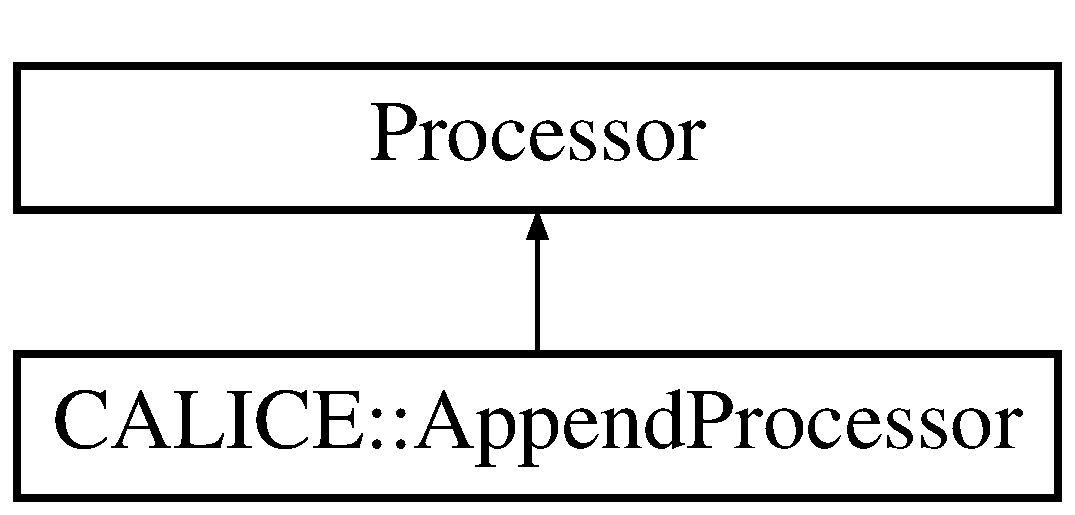
\includegraphics[height=2.000000cm]{classCALICE_1_1AppendProcessor}
\end{center}
\end{figure}
\subsection*{Public Member Functions}
\begin{DoxyCompactItemize}
\item 
virtual Processor $\ast$ {\bfseries new\-Processor} ()\label{classCALICE_1_1AppendProcessor_a49551ee02f9d177c4d77a9c0248aba85}

\item 
virtual void {\bfseries init} ()\label{classCALICE_1_1AppendProcessor_ac589867ec7de2dee41f13db721261877}

\item 
virtual void {\bfseries process\-Event} (lcio\-::\-L\-C\-Event $\ast$evt)\label{classCALICE_1_1AppendProcessor_ab5b4a17cc986692a45f4d6e748df08ee}

\end{DoxyCompactItemize}
\subsection*{Protected Types}
\begin{DoxyCompactItemize}
\item 
enum {\bfseries Hits\-Type\-\_\-t} \{ {\bfseries T\-C\-M\-T\-H\-I\-T}, 
{\bfseries F\-A\-S\-T\-C\-A\-L\-I\-C\-E\-H\-I\-T}
 \}
\end{DoxyCompactItemize}
\subsection*{Protected Attributes}
\begin{DoxyCompactItemize}
\item 
lcio\-::\-String\-Vec {\bfseries \-\_\-append\-File\-Names}\label{classCALICE_1_1AppendProcessor_afdd4ad0e4dada93d7d01c3f7632ab52f}

\item 
lcio\-::\-String\-Vec {\bfseries \-\_\-append\-Collection\-Input\-Names}\label{classCALICE_1_1AppendProcessor_adaa30643ff06a2922ba6150d0074a209}

\item 
lcio\-::\-String\-Vec {\bfseries \-\_\-append\-Collection\-Output\-Names}\label{classCALICE_1_1AppendProcessor_a587c513c73ccba16381895637ea7a573}

\item 
lcio\-::\-Int\-Vec {\bfseries \-\_\-append\-Collection\-Fix\-Levels}\label{classCALICE_1_1AppendProcessor_aeffce05dc4e7e46b4b6f8255bc25b087}

\item 
lcio\-::\-L\-C\-Reader $\ast$ {\bfseries \-\_\-lc\-Reader}\label{classCALICE_1_1AppendProcessor_af05bb76ed964d8ea1834a757bd6ea9f6}

\item 
lcio\-::\-Int\-Vec {\bfseries \-\_\-use\-Tcmt\-Hits}\label{classCALICE_1_1AppendProcessor_a7970df457e270143908dd9a3b79b39b1}

\item 
Hits\-Type\-\_\-t {\bfseries \-\_\-hits\-Type}\label{classCALICE_1_1AppendProcessor_ad93eefa5222ef45a3715c19eaa8ce2de}

\item 
bool {\bfseries \-\_\-append\-Repeat\-Collections}\label{classCALICE_1_1AppendProcessor_a82e205bebcae4791e97857b1b548ff28}

\end{DoxyCompactItemize}


\subsection{Detailed Description}
Processor which allows to append events from additional L\-C\-I\-O files. 

\begin{DoxyAuthor}{Authors}
Sebastian Schmidt, Joergen Samson, Guilherme Lima, Sebastian Richter 
\end{DoxyAuthor}
\begin{DoxyVersion}{Version}
1.\-0 
\end{DoxyVersion}


Definition at line 16 of file Append\-Processor.\-hh.



The documentation for this class was generated from the following files\-:\begin{DoxyCompactItemize}
\item 
Append\-Processor.\-hh\item 
Append\-Processor.\-cc\end{DoxyCompactItemize}

\section{bottom\-Both Class Reference}
\label{classbottomBoth}\index{bottom\-Both@{bottom\-Both}}


Implementation of ganger.  


Inheritance diagram for bottom\-Both\-:\begin{figure}[H]
\begin{center}
\leavevmode
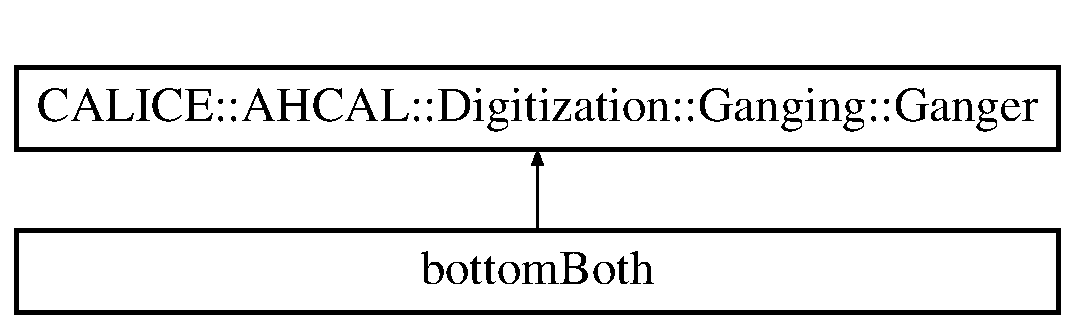
\includegraphics[height=2.000000cm]{classbottomBoth}
\end{center}
\end{figure}
\subsection*{Public Member Functions}
\begin{DoxyCompactItemize}
\item 
{\bfseries bottom\-Both} ({\bf Contribution\-Map} $\ast$cm, float factor)\label{classbottomBoth_a06933e621a94f172404ecc203acf5ac5}

\item 
bool {\bf responsible} ({\bf Geometrical\-Indices} indices)\label{classbottomBoth_abd6e0e0a8c5df530afc54e4fc43388ad}

\begin{DoxyCompactList}\small\item\em Implementations have to implement where in I/\-J they are responsible. \end{DoxyCompactList}\end{DoxyCompactItemize}


\subsection{Detailed Description}
Implementation of ganger. 

Definition at line 134 of file ahcal\-Ganging\-Processor.\-cc.



The documentation for this class was generated from the following file\-:\begin{DoxyCompactItemize}
\item 
ahcal\-Ganging\-Processor.\-cc\end{DoxyCompactItemize}

\section{Cal\-Hit\-Map\-Mgr Class Reference}
\label{classCalHitMapMgr}\index{Cal\-Hit\-Map\-Mgr@{Cal\-Hit\-Map\-Mgr}}
\subsection*{Public Member Functions}
\begin{DoxyCompactItemize}
\item 
void {\bfseries set\-Event} (E\-V\-E\-N\-T\-::\-L\-C\-Event \&event)\label{classCalHitMapMgr_ad3aaa8d5ae1478e9f52f05f209488fb3}

\item 
const Cal\-Hit\-Map \& {\bfseries get\-Coll\-Hit\-Map} (const std\-::string \&col\-Name)\label{classCalHitMapMgr_ae2a074496237dafdce69548f286369ae}

\end{DoxyCompactItemize}
\subsection*{Static Public Member Functions}
\begin{DoxyCompactItemize}
\item 
static {\bf Cal\-Hit\-Map\-Mgr} $\ast$ {\bfseries get\-Instance} ()\label{classCalHitMapMgr_a874f784c6a758bd9955da367d360edbc}

\item 
static void {\bfseries destroy} ()\label{classCalHitMapMgr_a7594e4c6027470927b332aa640e5d691}

\end{DoxyCompactItemize}
\subsection*{Private Member Functions}
\begin{DoxyCompactItemize}
\item 
void {\bfseries reset} ()\label{classCalHitMapMgr_a21bcf7abf7542fd01dcaec0db7479d9c}

\item 
void {\bfseries fill\-Hit\-Map} (const std\-::string \&col\-Name, Cal\-Hit\-Map \&hitmap)\label{classCalHitMapMgr_a60d1d1557559b96ad5ccbdf445c261f4}

\end{DoxyCompactItemize}
\subsection*{Private Attributes}
\begin{DoxyCompactItemize}
\item 
E\-V\-E\-N\-T\-::\-L\-C\-Event $\ast$ {\bfseries \-\_\-event}\label{classCalHitMapMgr_aa525fbd232694ae809c61eb4dd5e6048}

\item 
int {\bfseries \-\_\-runno}\label{classCalHitMapMgr_a2d631e3c16083f00bf82ebecec2f809c}

\item 
int {\bfseries \-\_\-evtno}\label{classCalHitMapMgr_a7cb32f55ac08d4020495787b1a35a03d}

\item 
Cal\-Hit\-Map {\bfseries \-\_\-em\-Hits}\label{classCalHitMapMgr_ad7eb8893b8b58013bf7af9ff96c6dacd}

\item 
Cal\-Hit\-Map {\bfseries \-\_\-had\-Hits}\label{classCalHitMapMgr_a9c2627d8456cc339d0e8ed02760c809c}

\item 
Cal\-Hit\-Collections {\bfseries \-\_\-coll\-Map}\label{classCalHitMapMgr_ab2218c79ccb9f434bace784e2aed2324}

\end{DoxyCompactItemize}
\subsection*{Static Private Attributes}
\begin{DoxyCompactItemize}
\item 
static {\bf Cal\-Hit\-Map\-Mgr} $\ast$ {\bfseries \-\_\-me} = N\-U\-L\-L\label{classCalHitMapMgr_a99b8aa53524ca9811a7a0d32684a1aee}

\end{DoxyCompactItemize}


\subsection{Detailed Description}


Definition at line 29 of file Cal\-Hit\-Map\-Mgr.\-hpp.



The documentation for this class was generated from the following files\-:\begin{DoxyCompactItemize}
\item 
Cal\-Hit\-Map\-Mgr.\-hpp\item 
Cal\-Hit\-Map\-Mgr.\-cpp\end{DoxyCompactItemize}

\section{digisim\-:\-:Cal\-Hit\-Map\-Processor Class Reference}
\label{classdigisim_1_1CalHitMapProcessor}\index{digisim\-::\-Cal\-Hit\-Map\-Processor@{digisim\-::\-Cal\-Hit\-Map\-Processor}}
Inheritance diagram for digisim\-:\-:Cal\-Hit\-Map\-Processor\-:\begin{figure}[H]
\begin{center}
\leavevmode
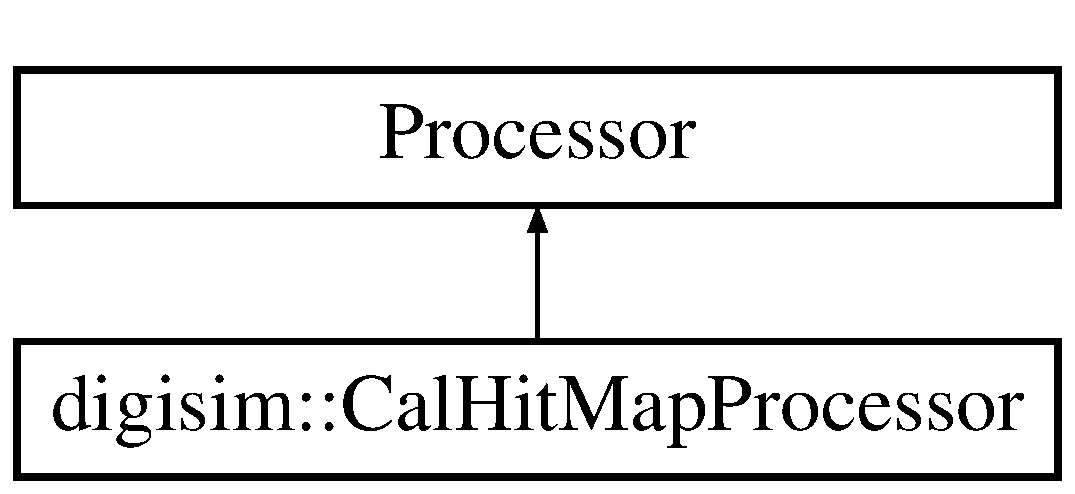
\includegraphics[height=2.000000cm]{classdigisim_1_1CalHitMapProcessor}
\end{center}
\end{figure}
\subsection*{Public Member Functions}
\begin{DoxyCompactItemize}
\item 
virtual Processor $\ast$ {\bfseries new\-Processor} ()\label{classdigisim_1_1CalHitMapProcessor_ab73604653fce83a5209b3155f971a266}

\item 
virtual void {\bf init} ()
\begin{DoxyCompactList}\small\item\em Called at the begin of the job before anything is read. \end{DoxyCompactList}\item 
virtual void {\bf process\-Run\-Header} (L\-C\-Run\-Header $\ast$run)\label{classdigisim_1_1CalHitMapProcessor_a9493177bc62f7a9489fc24230776617d}

\begin{DoxyCompactList}\small\item\em Called for every run. \end{DoxyCompactList}\item 
virtual void {\bf process\-Event} (L\-C\-Event $\ast$evt)\label{classdigisim_1_1CalHitMapProcessor_a9bfab5f8e22f049d0aae224e1cb862dd}

\begin{DoxyCompactList}\small\item\em Called for every event -\/ the working horse. \end{DoxyCompactList}\item 
virtual void {\bf end} ()\label{classdigisim_1_1CalHitMapProcessor_a7ed5be820bbe9b75023a173dadd41143}

\begin{DoxyCompactList}\small\item\em Called after data processing for clean up. \end{DoxyCompactList}\end{DoxyCompactItemize}
\subsection*{Protected Attributes}
\begin{DoxyCompactItemize}
\item 
int {\bfseries \-\_\-n\-Run}\label{classdigisim_1_1CalHitMapProcessor_a0b8bc56d5be22a8591a6364053a15d74}

\item 
int {\bfseries \-\_\-n\-Evt}\label{classdigisim_1_1CalHitMapProcessor_a3d9382829ccd70fab182453fb20f8ea7}

\item 
{\bf Cal\-Hit\-Map\-Mgr} $\ast$ {\bfseries \-\_\-mgr}\label{classdigisim_1_1CalHitMapProcessor_a361ac885c84aab286722fb9f3357c1ed}

\end{DoxyCompactItemize}


\subsection{Detailed Description}


Definition at line 30 of file Cal\-Hit\-Map\-Processor.\-hpp.



\subsection{Member Function Documentation}
\index{digisim\-::\-Cal\-Hit\-Map\-Processor@{digisim\-::\-Cal\-Hit\-Map\-Processor}!init@{init}}
\index{init@{init}!digisim::CalHitMapProcessor@{digisim\-::\-Cal\-Hit\-Map\-Processor}}
\subsubsection[{init}]{\setlength{\rightskip}{0pt plus 5cm}virtual void digisim\-::\-Cal\-Hit\-Map\-Processor\-::init (
\begin{DoxyParamCaption}
{}
\end{DoxyParamCaption}
)\hspace{0.3cm}{\ttfamily [inline]}, {\ttfamily [virtual]}}\label{classdigisim_1_1CalHitMapProcessor_a8709fbee06c74874da1850bc01e05765}


Called at the begin of the job before anything is read. 

Use to initialize the processor, e.\-g. book histograms. 

Definition at line 44 of file Cal\-Hit\-Map\-Processor.\-hpp.



The documentation for this class was generated from the following files\-:\begin{DoxyCompactItemize}
\item 
Cal\-Hit\-Map\-Processor.\-hpp\item 
Cal\-Hit\-Map\-Processor.\-cpp\end{DoxyCompactItemize}

\section{digisim\-:\-:Cal\-Hit\-Modifier Class Reference}
\label{classdigisim_1_1CalHitModifier}\index{digisim\-::\-Cal\-Hit\-Modifier@{digisim\-::\-Cal\-Hit\-Modifier}}
Inheritance diagram for digisim\-:\-:Cal\-Hit\-Modifier\-:\begin{figure}[H]
\begin{center}
\leavevmode
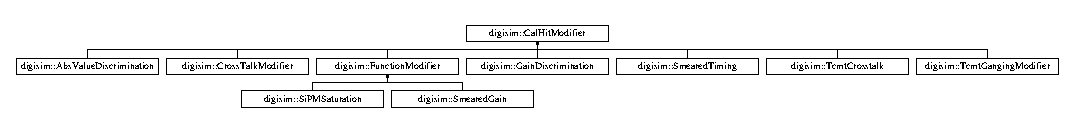
\includegraphics[height=1.212121cm]{classdigisim_1_1CalHitModifier}
\end{center}
\end{figure}
\subsection*{Public Member Functions}
\begin{DoxyCompactItemize}
\item 
virtual {\bf Cal\-Hit\-Modifier} $\ast$ {\bfseries new\-Instance} (const std\-::string \&mod\-Name)=0\label{classdigisim_1_1CalHitModifier_a78f014f6849ab103ddbe94093db157ff}

\item 
virtual void {\bfseries set\-Debug} (int deb)\label{classdigisim_1_1CalHitModifier_a40b3f84abd58a31f5f7c755f3289b68d}

\item 
virtual void {\bfseries init} (std\-::vector$<$ float $>$ \&floats)=0\label{classdigisim_1_1CalHitModifier_aa42345de981ae1c1be57db93f3d0870b}

\item 
virtual void {\bfseries process\-Hits} (Temp\-Cal\-Hit\-Map \&hitmap)=0\label{classdigisim_1_1CalHitModifier_a26d09ac955c90b605d14be89da08b1f3}

\item 
virtual void {\bfseries print} () const =0\label{classdigisim_1_1CalHitModifier_ae0f77ccebc8851ea8f9867b6ba5c6aa6}

\end{DoxyCompactItemize}
\subsection*{Static Public Attributes}
\begin{DoxyCompactItemize}
\item 
static std\-::map$<$ std\-::string, \\*
{\bf Cal\-Hit\-Modifier} $\ast$ $>$ {\bfseries \-\_\-modifiers\-Available}\label{classdigisim_1_1CalHitModifier_a08096a0d105eb7415212805c6312b9db}

\end{DoxyCompactItemize}
\subsection*{Protected Member Functions}
\begin{DoxyCompactItemize}
\item 
{\bfseries Cal\-Hit\-Modifier} (const std\-::string \&mod\-Name)\label{classdigisim_1_1CalHitModifier_ad342fac586ba1bb42049f4f91880ea8a}

\end{DoxyCompactItemize}
\subsection*{Static Protected Member Functions}
\begin{DoxyCompactItemize}
\item 
static void {\bfseries register\-Modifier} (const std\-::string \&name, {\bf Cal\-Hit\-Modifier} $\ast$p\-Mod)\label{classdigisim_1_1CalHitModifier_a406b5226b448efcd0b3ef0027087b70c}

\end{DoxyCompactItemize}
\subsection*{Protected Attributes}
\begin{DoxyCompactItemize}
\item 
int {\bfseries \-\_\-debug}\label{classdigisim_1_1CalHitModifier_a6995b37aaaf3f1e9a6b0d125d0af6dd5}

\item 
const std\-::string {\bfseries \-\_\-name}\label{classdigisim_1_1CalHitModifier_a121de4a7e029ba9c96cfd2c93b7d3017}

\end{DoxyCompactItemize}


\subsection{Detailed Description}


Definition at line 25 of file Cal\-Hit\-Modifier.\-hpp.



The documentation for this class was generated from the following files\-:\begin{DoxyCompactItemize}
\item 
Cal\-Hit\-Modifier.\-hpp\item 
Globals.\-cpp\end{DoxyCompactItemize}

\section{digisim\-:\-:Calorimeter\-Hits\-Processor Class Reference}
\label{classdigisim_1_1CalorimeterHitsProcessor}\index{digisim\-::\-Calorimeter\-Hits\-Processor@{digisim\-::\-Calorimeter\-Hits\-Processor}}
Inheritance diagram for digisim\-:\-:Calorimeter\-Hits\-Processor\-:\begin{figure}[H]
\begin{center}
\leavevmode
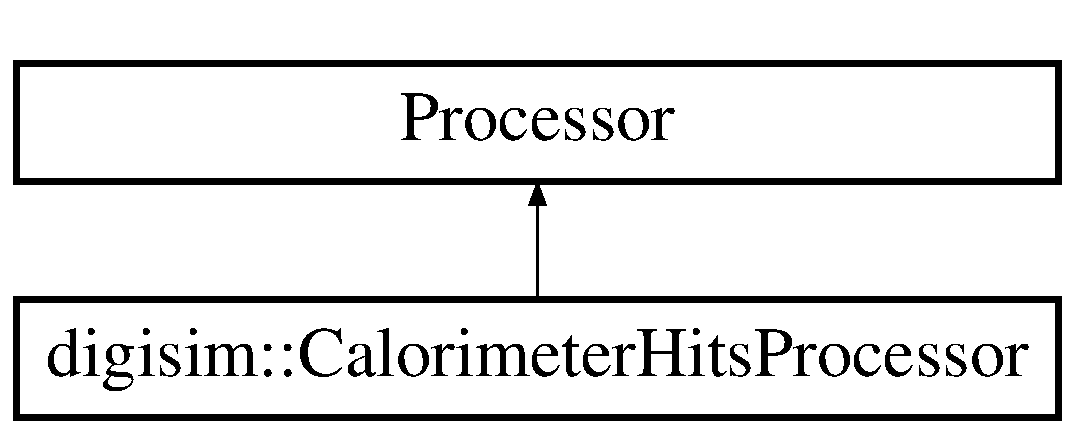
\includegraphics[height=2.000000cm]{classdigisim_1_1CalorimeterHitsProcessor}
\end{center}
\end{figure}
\subsection*{Public Member Functions}
\begin{DoxyCompactItemize}
\item 
virtual Processor $\ast$ {\bfseries new\-Processor} ()\label{classdigisim_1_1CalorimeterHitsProcessor_abf3f9e4ed0166c8ef1104708ed06260c}

\item 
virtual void {\bf init} ()
\begin{DoxyCompactList}\small\item\em Called at the begin of the job before anything is read. \end{DoxyCompactList}\item 
virtual void {\bf process\-Event} (L\-C\-Event $\ast$evt)
\begin{DoxyCompactList}\small\item\em Called for every run. \end{DoxyCompactList}\item 
virtual void {\bf end} ()\label{classdigisim_1_1CalorimeterHitsProcessor_ab6c5052db5b790dfed45d26255bb2b71}

\begin{DoxyCompactList}\small\item\em Called after data processing for clean up. \end{DoxyCompactList}\end{DoxyCompactItemize}
\subsection*{Protected Attributes}
\begin{DoxyCompactItemize}
\item 
L\-C\-Event $\ast$ {\bfseries \-\_\-evt}\label{classdigisim_1_1CalorimeterHitsProcessor_a4ea90da4b6e3c1d305027db644f8bb37}

\item 
std\-::string {\bfseries \-\_\-raw\-Name}\label{classdigisim_1_1CalorimeterHitsProcessor_a48525e77a89f66bb493fb14c0b28b475}

\item 
std\-::string {\bfseries \-\_\-output\-Name}\label{classdigisim_1_1CalorimeterHitsProcessor_a05771a12d33a36e49d65bc2303617003}

\item 
std\-::string {\bfseries \-\_\-pos\-Ref\-Name}\label{classdigisim_1_1CalorimeterHitsProcessor_a58758649ca1a759f27663b986085be32}

\item 
double {\bfseries \-\_\-ene\-Factor}\label{classdigisim_1_1CalorimeterHitsProcessor_af275a3b7cf25f25719d050595e421fdf}

\item 
double {\bfseries \-\_\-time\-Factor}\label{classdigisim_1_1CalorimeterHitsProcessor_a2987fffdc3d1ca312fef905f5073aa27}

\item 
int {\bfseries \-\_\-n\-Run}\label{classdigisim_1_1CalorimeterHitsProcessor_a3e43e1cd745608ee10c113c25d60c44b}

\item 
int {\bfseries \-\_\-n\-Evt}\label{classdigisim_1_1CalorimeterHitsProcessor_a861f268ec460f2ab7658971738c3b672}

\item 
bool {\bfseries \-\_\-positions\-From\-File}\label{classdigisim_1_1CalorimeterHitsProcessor_a87e4b7b02c9627fe7816b9c5b8eb9c59}

\item 
bool {\bfseries \-\_\-defer\-Position\-Assignments}\label{classdigisim_1_1CalorimeterHitsProcessor_ad9c012c16278fdf4d7585addf8a017e4}

\item 
std\-::map$<$ long long, \\*
std\-::vector$<$ double $>$ $>$ {\bfseries \-\_\-positions\-Map}\label{classdigisim_1_1CalorimeterHitsProcessor_a12d9128f4082932e8fdb1ad9d6a71201}

\item 
{\bf Raw\-Hit\-Converter} $\ast$ {\bfseries \-\_\-converter}\label{classdigisim_1_1CalorimeterHitsProcessor_a9a52fc987bf426d6756a73541f09116c}

\end{DoxyCompactItemize}
\subsection*{Private Member Functions}
\begin{DoxyCompactItemize}
\item 
E\-V\-E\-N\-T\-::\-L\-C\-Collection $\ast$ {\bfseries create\-Output\-Collection} (const std\-::vector$<$ const I\-M\-P\-L\-::\-Calorimeter\-Hit\-Impl $\ast$ $>$ \&newhits)\label{classdigisim_1_1CalorimeterHitsProcessor_a5fb2566100dc2146f7eacca0fc8b2675}

\end{DoxyCompactItemize}


\subsection{Detailed Description}


Definition at line 23 of file Calorimeter\-Hits\-Processor.\-hpp.



\subsection{Member Function Documentation}
\index{digisim\-::\-Calorimeter\-Hits\-Processor@{digisim\-::\-Calorimeter\-Hits\-Processor}!init@{init}}
\index{init@{init}!digisim::CalorimeterHitsProcessor@{digisim\-::\-Calorimeter\-Hits\-Processor}}
\subsubsection[{init}]{\setlength{\rightskip}{0pt plus 5cm}void digisim\-::\-Calorimeter\-Hits\-Processor\-::init (
\begin{DoxyParamCaption}
{}
\end{DoxyParamCaption}
)\hspace{0.3cm}{\ttfamily [virtual]}}\label{classdigisim_1_1CalorimeterHitsProcessor_a12a2d931a291eeea93c9c97a72bffba3}


Called at the begin of the job before anything is read. 

Use to initialize the processor, e.\-g. book histograms. 

Definition at line 189 of file Calorimeter\-Hits\-Processor.\-cpp.

\index{digisim\-::\-Calorimeter\-Hits\-Processor@{digisim\-::\-Calorimeter\-Hits\-Processor}!process\-Event@{process\-Event}}
\index{process\-Event@{process\-Event}!digisim::CalorimeterHitsProcessor@{digisim\-::\-Calorimeter\-Hits\-Processor}}
\subsubsection[{process\-Event}]{\setlength{\rightskip}{0pt plus 5cm}void digisim\-::\-Calorimeter\-Hits\-Processor\-::process\-Event (
\begin{DoxyParamCaption}
\item[{L\-C\-Event $\ast$}]{evt}
\end{DoxyParamCaption}
)\hspace{0.3cm}{\ttfamily [virtual]}}\label{classdigisim_1_1CalorimeterHitsProcessor_aea76b4b369097dd0872d334ea7a2b438}


Called for every run. 

Called for every event 

Definition at line 78 of file Calorimeter\-Hits\-Processor.\-cpp.



The documentation for this class was generated from the following files\-:\begin{DoxyCompactItemize}
\item 
Calorimeter\-Hits\-Processor.\-hpp\item 
Calorimeter\-Hits\-Processor.\-cpp\end{DoxyCompactItemize}

\section{Cell\-I\-D\-Decoder\-:\-:cell\-I\-D Struct Reference}
\label{structCellIDDecoder_1_1cellID}\index{Cell\-I\-D\-Decoder\-::cell\-I\-D@{Cell\-I\-D\-Decoder\-::cell\-I\-D}}
\subsection*{Data Fields}
\begin{DoxyCompactItemize}
\item 
unsigned int {\bfseries id0}\label{structCellIDDecoder_1_1cellID_a3ce25128462b7f1a02f793444d97b825}

\item 
unsigned int {\bfseries id1}\label{structCellIDDecoder_1_1cellID_a2b718a8f0cfc9b9eae6c87a23c2a9411}

\end{DoxyCompactItemize}


\subsection{Detailed Description}


Definition at line 25 of file Cell\-I\-D\-Decoder.\-hpp.



The documentation for this struct was generated from the following file\-:\begin{DoxyCompactItemize}
\item 
Cell\-I\-D\-Decoder.\-hpp\end{DoxyCompactItemize}

\section{Cell\-I\-D\-Decoder Class Reference}
\label{classCellIDDecoder}\index{Cell\-I\-D\-Decoder@{Cell\-I\-D\-Decoder}}
\subsection*{Data Structures}
\begin{DoxyCompactItemize}
\item 
struct {\bf cell\-I\-D}
\item 
class {\bf decoder}
\end{DoxyCompactItemize}
\subsection*{Public Member Functions}
\begin{DoxyCompactItemize}
\item 
{\bfseries Cell\-I\-D\-Decoder} (const int cell\-I\-D0, const int cell\-I\-D1, int Symmetry\-Order)\label{classCellIDDecoder_a57a59e864743d82a3f17eba130e0c158}

\item 
{\bfseries Cell\-I\-D\-Decoder} (long long {\bf cell\-I\-D}, int Symmetry\-Order, bool use\-Encoder32)\label{classCellIDDecoder_a724b4bba1fb1621ac12a0554d07c513e}

\item 
{\bfseries Cell\-I\-D\-Decoder} (int cell\-I\-D0, int Symmetry\-Order)\label{classCellIDDecoder_a6a1beb6f05b1ce3380e5b7c648171eff}

\item 
{\bfseries Cell\-I\-D\-Decoder} (int Symmetry\-Order, bool use\-Encoder32)\label{classCellIDDecoder_a7a0313f2e451e3bcea401b2c98eb28c6}

\item 
int {\bf get\-L1} () const \label{classCellIDDecoder_afa98ebb29126d5e8c98a218862fe641d}

\begin{DoxyCompactList}\small\item\em Symmetry\-Order is the order of the rotational symmetry \par
 8 for an octagonal barrel calorimeter\par
 2 for an endcap calorimeter\par
 1 for a standalone prototype\par
 0 for an idealized cylindrical calorimeter. \end{DoxyCompactList}\item 
int {\bfseries get\-L2} () const \label{classCellIDDecoder_a1a942f4c597b2ba63614fd0f5366fa26}

\item 
int {\bfseries get\-Prov} () const \label{classCellIDDecoder_ad111007ae3b5976c2c4de1641daa6120}

\item 
int {\bfseries get\-K} () const \label{classCellIDDecoder_a9b778944dc142f161a4338b883e0ae4a}

\item 
int {\bfseries get\-M} () const \label{classCellIDDecoder_af4e7450a2bde36ed410c824918327c3b}

\item 
int {\bfseries get\-S} () const \label{classCellIDDecoder_a12262c7a0ba9c0d98a30cff42fa1e86c}

\item 
int {\bfseries get\-I} () const \label{classCellIDDecoder_a7178a0e8fca513f2c63b072a7d1ef031}

\item 
int {\bfseries get\-J} () const \label{classCellIDDecoder_aa2ccda21c1eda20d8cfb49d5b095e7bb}

\item 
int {\bfseries get\-Imax} () const \label{classCellIDDecoder_ac7f29623ab8a976a2e1a3a433a386da4}

\item 
int {\bfseries get\-Jmax} () const \label{classCellIDDecoder_a75a5dadf8c8a13099078e5cc5878f763}

\item 
int {\bfseries get\-K\-S\-M} () const \label{classCellIDDecoder_a10b875d5861db0e62b01fa5d78691e82}

\item 
int {\bfseries get\-G\-R\-Zone} () const \label{classCellIDDecoder_a58d5ee7717684a20890d7cdca28b1861}

\item 
int {\bfseries is\-Same\-Wafer} (const {\bf Cell\-I\-D\-Decoder} \&neighbour)\label{classCellIDDecoder_a4297eb41dc656f43e003e71a15ca872d}

\item 
int {\bfseries get\-I} (int N\-C\-E\-L\-L\-S)\label{classCellIDDecoder_a0f1d29c476fc382f9c8d8ed66c5a9940}

\item 
int {\bfseries get\-J} (int N\-C\-E\-L\-L\-S)\label{classCellIDDecoder_ac49dea91b9e9b89aa017c57d554b6abd}

\item 
std\-::pair$<$ int, int $>$ {\bfseries Encode} ()\label{classCellIDDecoder_a6b686fd95782c17d6ac3b5e23ff78973}

\item 
std\-::pair$<$ int, int $>$ {\bfseries Encode} (int N\-C\-E\-L\-L\-S)\label{classCellIDDecoder_a985d59486ee5905edb133bc913e3b6cf}

\item 
std\-::pair$<$ int, int $>$ {\bfseries Encode} (int K, int S, int M, int I, int J)\label{classCellIDDecoder_a798ce6ff231fc70e904cd20d23a37210}

\item 
long long {\bfseries Encode\-Neigh} (int deltai, int deltaj, int N\-C\-E\-L\-L\-S)\label{classCellIDDecoder_a01a1621bdb246bbf8100d34e0ab2983e}

\item 
long long {\bfseries Encode\-Neigh} (int deltai, int deltaj)\label{classCellIDDecoder_adbeab7f1741e44595dd06616fdca8a1f}

\end{DoxyCompactItemize}
\subsection*{Static Public Member Functions}
\begin{DoxyCompactItemize}
\item 
static const {\bf decoder} \& {\bfseries Get\-Decoder} ()\label{classCellIDDecoder_af27dfed8b6ba27ad29070cc709cd1dc2}

\end{DoxyCompactItemize}
\subsection*{Private Attributes}
\begin{DoxyCompactItemize}
\item 
{\bf cell\-I\-D} {\bfseries \-\_\-mycell\-I\-D}\label{classCellIDDecoder_a80eb4e813fdba53afd6eabe36881be62}

\item 
bool {\bfseries \-\_\-is32}\label{classCellIDDecoder_a562e6de1c58e67548ab7aae2b3ab6371}

\item 
int {\bfseries \-\_\-symmetry\-Order}\label{classCellIDDecoder_a60d27aa7ada2fb0cdb35357803924f2c}

\item 
const int $\ast$ {\bfseries p\-\_\-mask}\label{classCellIDDecoder_a22de1f2756130010bd9a3aa55516cc5f}

\item 
const int $\ast$ {\bfseries p\-\_\-shift}\label{classCellIDDecoder_aa5c90c05a46e982aba9e50082239f2fc}

\end{DoxyCompactItemize}


\subsection{Detailed Description}


Definition at line 6 of file Cell\-I\-D\-Decoder.\-hpp.



The documentation for this class was generated from the following files\-:\begin{DoxyCompactItemize}
\item 
Cell\-I\-D\-Decoder.\-hpp\item 
Cell\-I\-D\-Decoder.\-cpp\end{DoxyCompactItemize}

\section{digisim\-:\-:Cross\-Talk\-Modifier Class Reference}
\label{classdigisim_1_1CrossTalkModifier}\index{digisim\-::\-Cross\-Talk\-Modifier@{digisim\-::\-Cross\-Talk\-Modifier}}
Inheritance diagram for digisim\-:\-:Cross\-Talk\-Modifier\-:\begin{figure}[H]
\begin{center}
\leavevmode
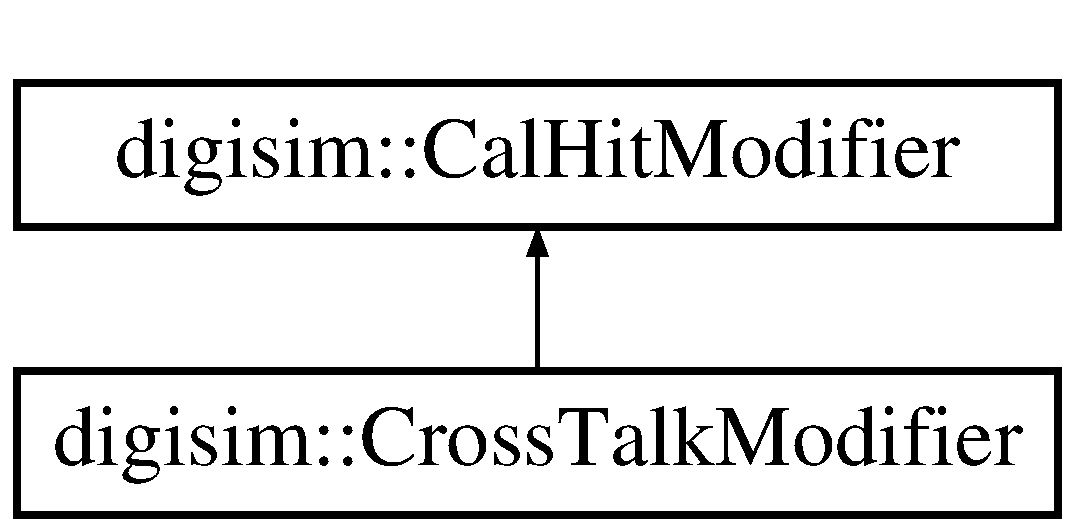
\includegraphics[height=2.000000cm]{classdigisim_1_1CrossTalkModifier}
\end{center}
\end{figure}
\subsection*{Public Member Functions}
\begin{DoxyCompactItemize}
\item 
{\bf Cross\-Talk\-Modifier} $\ast$ {\bfseries new\-Instance} (const std\-::string \&mod\-Name)\label{classdigisim_1_1CrossTalkModifier_a815dbbbc6b62e59e26dc2837514a1170}

\item 
void {\bfseries init} (std\-::vector$<$ float $>$ \&floats)\label{classdigisim_1_1CrossTalkModifier_a0da6aa9e02508cd60634b5ca23d25f12}

\item 
void {\bfseries process\-Hits} (Temp\-Cal\-Hit\-Map \&hitmap)\label{classdigisim_1_1CrossTalkModifier_a7ce6493c5a974b37befa87bf2678e934}

\item 
void {\bfseries print} () const \label{classdigisim_1_1CrossTalkModifier_a8e085d278314de45acf7bcc983eefb0d}

\end{DoxyCompactItemize}
\subsection*{Private Member Functions}
\begin{DoxyCompactItemize}
\item 
{\bfseries Cross\-Talk\-Modifier} (const std\-::string \&mod\-Name)\label{classdigisim_1_1CrossTalkModifier_afff4eb14b9f944e69a91fde00dda72a5}

\item 
{\bfseries Cross\-Talk\-Modifier} (const {\bf Cross\-Talk\-Modifier} \&rhs)\label{classdigisim_1_1CrossTalkModifier_a21f2c0a9185904b8bf56738d40e67985}

\end{DoxyCompactItemize}
\subsection*{Private Attributes}
\begin{DoxyCompactItemize}
\item 
std\-::vector$<$ float $>$ {\bfseries \-\_\-par}\label{classdigisim_1_1CrossTalkModifier_a26a02dd37217a1ce402ef167aabfcb5b}

\end{DoxyCompactItemize}
\subsection*{Additional Inherited Members}


\subsection{Detailed Description}


Definition at line 19 of file Cross\-Talk\-Modifier.\-hpp.



The documentation for this class was generated from the following files\-:\begin{DoxyCompactItemize}
\item 
Cross\-Talk\-Modifier.\-hpp\item 
Cross\-Talk\-Modifier.\-cpp\end{DoxyCompactItemize}

\section{Cell\-I\-D\-Decoder\-:\-:decoder Class Reference}
\label{classCellIDDecoder_1_1decoder}\index{Cell\-I\-D\-Decoder\-::decoder@{Cell\-I\-D\-Decoder\-::decoder}}
\subsection*{Private Attributes}
\begin{DoxyCompactItemize}
\item 
int {\bfseries mask\-\_\-32} [8]\label{classCellIDDecoder_1_1decoder_a42b09663e93c2f46fa72e2b2de6edd6b}

\item 
int {\bfseries shift\-\_\-32} [8]\label{classCellIDDecoder_1_1decoder_a14beea35350f8107e69634dbb32fc920}

\item 
int {\bfseries mask\-\_\-64} [10]\label{classCellIDDecoder_1_1decoder_a80ae287b494692d309632d6d718f5589}

\item 
int {\bfseries shift\-\_\-64} [10]\label{classCellIDDecoder_1_1decoder_a3ef5bc7c99e94f2d2c5b9b1cfbb99cc7}

\item 
int {\bfseries mask\-\_\-\-M\-A\-P\-S} [10]\label{classCellIDDecoder_1_1decoder_ae5fefd9a154215933e4fcd84a385ded8}

\item 
int {\bfseries shift\-\_\-\-M\-A\-P\-S} [10]\label{classCellIDDecoder_1_1decoder_a845f3872403b52830025328137b06c47}

\end{DoxyCompactItemize}
\subsection*{Friends}
\begin{DoxyCompactItemize}
\item 
class {\bfseries Cell\-I\-D\-Decoder}\label{classCellIDDecoder_1_1decoder_a9449cccf7753cfe2c5b4383443c25c59}

\end{DoxyCompactItemize}


\subsection{Detailed Description}


Definition at line 9 of file Cell\-I\-D\-Decoder.\-hpp.



The documentation for this class was generated from the following files\-:\begin{DoxyCompactItemize}
\item 
Cell\-I\-D\-Decoder.\-hpp\item 
Cell\-I\-D\-Decoder.\-cpp\end{DoxyCompactItemize}

\section{digisim\-:\-:Digi\-Sim\-Processor Class Reference}
\label{classdigisim_1_1DigiSimProcessor}\index{digisim\-::\-Digi\-Sim\-Processor@{digisim\-::\-Digi\-Sim\-Processor}}
Inheritance diagram for digisim\-:\-:Digi\-Sim\-Processor\-:\begin{figure}[H]
\begin{center}
\leavevmode
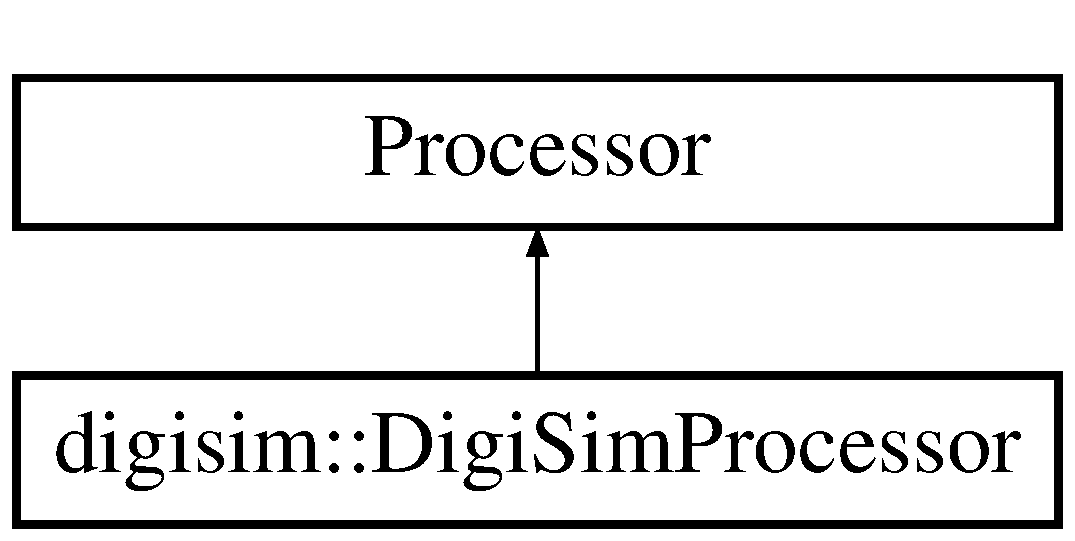
\includegraphics[height=2.000000cm]{classdigisim_1_1DigiSimProcessor}
\end{center}
\end{figure}
\subsection*{Public Member Functions}
\begin{DoxyCompactItemize}
\item 
virtual Processor $\ast$ {\bfseries new\-Processor} ()\label{classdigisim_1_1DigiSimProcessor_aa222ce6e8d8948c1d1c6dd413d3a0d45}

\item 
void {\bfseries print\-Relation} (const E\-V\-E\-N\-T\-::\-L\-C\-Collection $\ast$col) const \label{classdigisim_1_1DigiSimProcessor_a524cf1b360877b285cbe11775db8b24e}

\item 
virtual void {\bf init} ()
\begin{DoxyCompactList}\small\item\em Called at the begin of the job before anything is read. \end{DoxyCompactList}\item 
virtual void {\bf process\-Run\-Header} (L\-C\-Run\-Header $\ast$run)\label{classdigisim_1_1DigiSimProcessor_afebcfdc5cee837f85b936f1bb2755641}

\begin{DoxyCompactList}\small\item\em Called for every run. \end{DoxyCompactList}\item 
virtual void {\bf process\-Event} (L\-C\-Event $\ast$evt)\label{classdigisim_1_1DigiSimProcessor_a9871ae2646095074aa75eba727d3377a}

\begin{DoxyCompactList}\small\item\em Called for every event -\/ the working horse. \end{DoxyCompactList}\item 
virtual void {\bf end} ()\label{classdigisim_1_1DigiSimProcessor_a2028c0212bdad8abc1359f0a6652d1a4}

\begin{DoxyCompactList}\small\item\em Called after data processing for clean up. \end{DoxyCompactList}\end{DoxyCompactItemize}
\subsection*{Protected Attributes}
\begin{DoxyCompactItemize}
\item 
string {\bfseries diginame}\label{classdigisim_1_1DigiSimProcessor_a1f36e9a8e9f51d4138b194ae39e90344}

\item 
L\-C\-Writer $\ast$ {\bfseries \-\_\-lc\-Wrt}\label{classdigisim_1_1DigiSimProcessor_a775602d175432ad858eb44d3d2bfa8e9}

\item 
int {\bfseries \-\_\-n\-Run}\label{classdigisim_1_1DigiSimProcessor_ad02d718ca23c6918b78d56bc73170303}

\item 
int {\bfseries \-\_\-n\-Evt}\label{classdigisim_1_1DigiSimProcessor_a91a6f63de7603ee1d9fc13c95439cf4e}

\item 
int {\bfseries \-\_\-debug}\label{classdigisim_1_1DigiSimProcessor_af12d11d34e1b73e055a6f65fce61efd3}

\item 
std\-::list$<$ {\bf Cal\-Hit\-Modifier} $\ast$ $>$ {\bfseries \-\_\-modifs}\label{classdigisim_1_1DigiSimProcessor_a75b1fc16f09f7c3018a62a744f786663}

\item 
std\-::string {\bfseries \-\_\-input\-Coll}\label{classdigisim_1_1DigiSimProcessor_a4d79d468a8eaa78ee05c68df7c6b24d2}

\item 
std\-::string {\bfseries \-\_\-output\-Coll}\label{classdigisim_1_1DigiSimProcessor_a5b55fe6a6503cf31a89a066e96875057}

\item 
std\-::string {\bfseries \-\_\-links\-Coll}\label{classdigisim_1_1DigiSimProcessor_a99b2a5a5c2666d367b59eda5b1157a67}

\item 
std\-::vector$<$ std\-::string $>$ {\bfseries \-\_\-modif\-Names}\label{classdigisim_1_1DigiSimProcessor_ad1b9e146bff72901ef2f7714ff337185}

\item 
std\-::vector$<$ {\bf Digitizer} $>$ {\bfseries \-\_\-digitizers}\label{classdigisim_1_1DigiSimProcessor_a092b7a7d3a2311925a1ff343305f77ed}

\end{DoxyCompactItemize}


\subsection{Detailed Description}


Definition at line 29 of file Digi\-Sim\-Processor.\-hpp.



\subsection{Member Function Documentation}
\index{digisim\-::\-Digi\-Sim\-Processor@{digisim\-::\-Digi\-Sim\-Processor}!init@{init}}
\index{init@{init}!digisim::DigiSimProcessor@{digisim\-::\-Digi\-Sim\-Processor}}
\subsubsection[{init}]{\setlength{\rightskip}{0pt plus 5cm}void digisim\-::\-Digi\-Sim\-Processor\-::init (
\begin{DoxyParamCaption}
{}
\end{DoxyParamCaption}
)\hspace{0.3cm}{\ttfamily [virtual]}}\label{classdigisim_1_1DigiSimProcessor_a2ffa050ec7b4477cbce6da55a4a1d1e9}


Called at the begin of the job before anything is read. 

Use to initialize the processor, e.\-g. book histograms. 

Definition at line 90 of file Digi\-Sim\-Processor.\-cpp.



The documentation for this class was generated from the following files\-:\begin{DoxyCompactItemize}
\item 
Digi\-Sim\-Processor.\-hpp\item 
Digi\-Sim\-Processor.\-cpp\end{DoxyCompactItemize}

\section{digisim\-:\-:Digitizer Class Reference}
\label{classdigisim_1_1Digitizer}\index{digisim\-::\-Digitizer@{digisim\-::\-Digitizer}}
\subsection*{Public Member Functions}
\begin{DoxyCompactItemize}
\item 
{\bfseries Digitizer} (std\-::string name)\label{classdigisim_1_1Digitizer_af23f97bc436d7d882822fd5a46222ce2}

\item 
void {\bfseries init} (std\-::shared\-\_\-ptr$<$ marlin\-::\-String\-Parameters $>$ pars)\label{classdigisim_1_1Digitizer_a7b7ee64e5e0329f70c5d462d5dca5523}

\item 
void {\bfseries init} (std\-::vector$<$ std\-::string $>$ collnames, std\-::vector$<$ {\bf Modifier\-Parameters} $>$ modifiers)\label{classdigisim_1_1Digitizer_ab3e8c0b4a5a1773b44ce0ecd964298c8}

\item 
void {\bfseries init} (std\-::string in\-Coll, std\-::string out\-Coll, std\-::string links\-Coll, std\-::vector$<$ {\bf Modifier\-Parameters} $>$ modifiers)\label{classdigisim_1_1Digitizer_a9cda05b68efc291523f1ee9d268cb884}

\item 
void {\bf initialize} (std\-::vector$<$ {\bf Modifier\-Parameters} $>$ modifiers)
\begin{DoxyCompactList}\small\item\em Instantiate modifiers, assuming the collection names have been set. \end{DoxyCompactList}\item 
void {\bf process} (L\-C\-Event $\ast$evt)\label{classdigisim_1_1Digitizer_a7012daa4097d73f1cd21cf894e6ae1a7}

\begin{DoxyCompactList}\small\item\em Called for every event -\/ the event loop. \end{DoxyCompactList}\item 
void {\bfseries end} ()\label{classdigisim_1_1Digitizer_a40c49da9a558250ea248e462ef895c41}

\item 
std\-::string {\bfseries get\-Name} ()\label{classdigisim_1_1Digitizer_ad44b298e9395eb7a3c8a200fe9bd4efd}

\end{DoxyCompactItemize}
\subsection*{Private Member Functions}
\begin{DoxyCompactItemize}
\item 
std\-::map$<$ long long, {\bf Temp\-Cal\-Hit} $>$ {\bfseries create\-Temp\-Hits} (const Cal\-Hit\-Map \&sim\-Hits)\label{classdigisim_1_1Digitizer_a9ef8f3d94a3491b0221c166ae3820ff3}

\item 
void {\bfseries create\-Output\-Collections} (const std\-::map$<$ long long, {\bf Temp\-Cal\-Hit} $>$ tmp\-Hits, L\-C\-Collection $\ast$\&raw\-Vec, L\-C\-Collection $\ast$\&rel\-Vec)\label{classdigisim_1_1Digitizer_af22d9e764ba3aed8b5bbb5a17e5a62ce}

\end{DoxyCompactItemize}
\subsection*{Private Attributes}
\begin{DoxyCompactItemize}
\item 
int {\bfseries \-\_\-n\-Run}\label{classdigisim_1_1Digitizer_a4eefda52faaf6a17ef48c8b486ac2531}

\item 
int {\bfseries \-\_\-n\-Evt}\label{classdigisim_1_1Digitizer_aa49d78fa38014a642fb699cde8970e71}

\item 
int {\bfseries \-\_\-debug}\label{classdigisim_1_1Digitizer_a57011e6745ef3c1d0272514dee75fd18}

\item 
std\-::string {\bfseries \-\_\-name}\label{classdigisim_1_1Digitizer_ab193142fb498d1991aaf30671b9d6abd}

\item 
std\-::vector$<$ {\bf Cal\-Hit\-Modifier} $\ast$ $>$ {\bfseries \-\_\-modifs}\label{classdigisim_1_1Digitizer_a095d111a53880dfe3d2ab6bbadd38eb0}

\item 
std\-::string {\bfseries \-\_\-input\-Coll}\label{classdigisim_1_1Digitizer_afadeb603edea52f158b4201be28d578e}

\item 
std\-::string {\bfseries \-\_\-output\-Coll}\label{classdigisim_1_1Digitizer_ad3b522fb767939438f1137df2a551989}

\item 
std\-::string {\bfseries \-\_\-links\-Coll}\label{classdigisim_1_1Digitizer_ad9c673919cf20cdf1f4e39e6cabc9e91}

\end{DoxyCompactItemize}


\subsection{Detailed Description}


Definition at line 21 of file Digitizer.\-hpp.



\subsection{Member Function Documentation}
\index{digisim\-::\-Digitizer@{digisim\-::\-Digitizer}!initialize@{initialize}}
\index{initialize@{initialize}!digisim::Digitizer@{digisim\-::\-Digitizer}}
\subsubsection[{initialize}]{\setlength{\rightskip}{0pt plus 5cm}void digisim\-::\-Digitizer\-::initialize (
\begin{DoxyParamCaption}
\item[{std\-::vector$<$ {\bf Modifier\-Parameters} $>$}]{modifiers}
\end{DoxyParamCaption}
)}\label{classdigisim_1_1Digitizer_abd7040d86648e9006b28beb18161e294}


Instantiate modifiers, assuming the collection names have been set. 


\begin{DoxyParams}{Parameters}
{\em modifiers} & a vector with \doxyref{Modifier\-Parameters}{p.}{classdigisim_1_1ModifierParameters} objects. Each \doxyref{Modifier\-Parameters}{p.}{classdigisim_1_1ModifierParameters} object will be associated to its own modifier, creating a chain of modifiers for this digitizer. \\
\hline
\end{DoxyParams}


Definition at line 216 of file Digitizer.\-cpp.



The documentation for this class was generated from the following files\-:\begin{DoxyCompactItemize}
\item 
Digitizer.\-hpp\item 
Digitizer.\-cpp\end{DoxyCompactItemize}

\section{C\-A\-L\-I\-C\-E\-:\-:Error\-Missing\-Conditions\-Data\-Handler Class Reference}
\label{classCALICE_1_1ErrorMissingConditionsDataHandler}\index{C\-A\-L\-I\-C\-E\-::\-Error\-Missing\-Conditions\-Data\-Handler@{C\-A\-L\-I\-C\-E\-::\-Error\-Missing\-Conditions\-Data\-Handler}}
Inheritance diagram for C\-A\-L\-I\-C\-E\-:\-:Error\-Missing\-Conditions\-Data\-Handler\-:\begin{figure}[H]
\begin{center}
\leavevmode
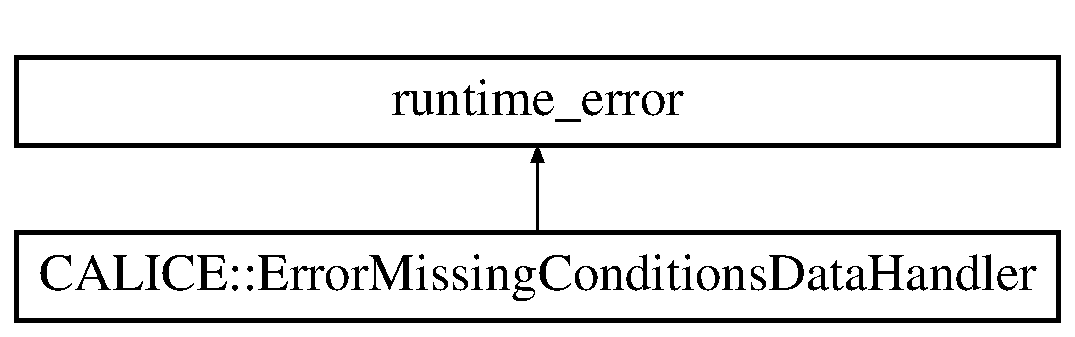
\includegraphics[height=1.021898cm]{classCALICE_1_1ErrorMissingConditionsDataHandler}
\end{center}
\end{figure}
\subsection*{Public Member Functions}
\begin{DoxyCompactItemize}
\item 
{\bfseries Error\-Missing\-Conditions\-Data\-Handler} (const std\-::string \&message)\label{classCALICE_1_1ErrorMissingConditionsDataHandler_a0a85b29547427c53f0c9f5ba5b3070b0}

\item 
{\bfseries Error\-Missing\-Conditions\-Data\-Handler} (const std\-::string \&message)\label{classCALICE_1_1ErrorMissingConditionsDataHandler_a0a85b29547427c53f0c9f5ba5b3070b0}

\item 
{\bfseries Error\-Missing\-Conditions\-Data\-Handler} (const std\-::string \&message)\label{classCALICE_1_1ErrorMissingConditionsDataHandler_a0a85b29547427c53f0c9f5ba5b3070b0}

\item 
{\bfseries Error\-Missing\-Conditions\-Data\-Handler} (const std\-::string \&message)\label{classCALICE_1_1ErrorMissingConditionsDataHandler_a0a85b29547427c53f0c9f5ba5b3070b0}

\end{DoxyCompactItemize}


\subsection{Detailed Description}


Definition at line 19 of file Base\-Mapping\-I\-I\-Processor.\-hh.



The documentation for this class was generated from the following files\-:\begin{DoxyCompactItemize}
\item 
Base\-Mapping\-I\-I\-Processor.\-hh\item 
fast\-Mapping\-I\-I\-Processor.\-hh\item 
Sc\-E\-C\-A\-L\-Mapping\-Processor.\-hh\item 
V\-Raw\-A\-D\-C\-Value\-Processor.\-hh\end{DoxyCompactItemize}

\section{C\-A\-L\-I\-C\-E\-:\-:fast\-Mapping\-M\-C\-Processor Class Reference}
\label{classCALICE_1_1fastMappingMCProcessor}\index{C\-A\-L\-I\-C\-E\-::fast\-Mapping\-M\-C\-Processor@{C\-A\-L\-I\-C\-E\-::fast\-Mapping\-M\-C\-Processor}}


A class which converts M\-C Calorimeter\-Hits to Calice\-Hits according to the hardware conditions.  




{\ttfamily \#include $<$fast\-Mapping\-M\-C\-Processor.\-hh$>$}

Inheritance diagram for C\-A\-L\-I\-C\-E\-:\-:fast\-Mapping\-M\-C\-Processor\-:\begin{figure}[H]
\begin{center}
\leavevmode
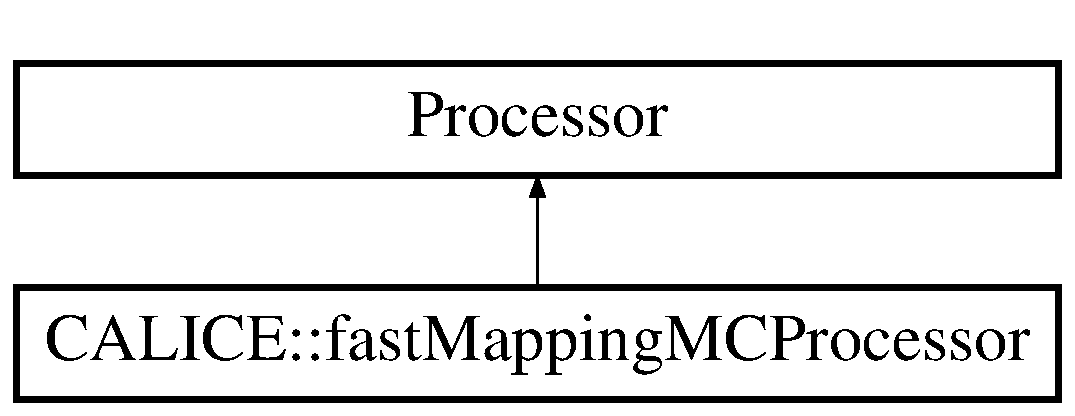
\includegraphics[height=2.000000cm]{classCALICE_1_1fastMappingMCProcessor}
\end{center}
\end{figure}
\subsection*{Public Member Functions}
\begin{DoxyCompactItemize}
\item 
virtual Processor $\ast$ {\bfseries new\-Processor} ()\label{classCALICE_1_1fastMappingMCProcessor_ab06a418d8f426b4f376038e15648f805}

\item 
virtual void {\bfseries init} ()\label{classCALICE_1_1fastMappingMCProcessor_ac553a3f1f37551ea82ec357033a94627}

\item 
virtual void {\bfseries process\-Event} (L\-C\-Event $\ast$evt)\label{classCALICE_1_1fastMappingMCProcessor_a421b8d6a2de101b449bd113174e765a3}

\end{DoxyCompactItemize}
\subsection*{Protected Member Functions}
\begin{DoxyCompactItemize}
\item 
virtual void {\bfseries module\-Type\-Changed} (lcio\-::\-L\-C\-Collection $\ast$col)\label{classCALICE_1_1fastMappingMCProcessor_ac8ab2a7a6f74c8431825a07f968cc5c8}

\item 
virtual void {\bfseries module\-Location\-Changed} (lcio\-::\-L\-C\-Collection $\ast$col)\label{classCALICE_1_1fastMappingMCProcessor_af1594c423e9d7594ac32dfa3aefed41a}

\item 
virtual void {\bfseries module\-Connection\-Changed} (lcio\-::\-L\-C\-Collection $\ast$col)\label{classCALICE_1_1fastMappingMCProcessor_a80ccd4b7f2477e2ef827150d26b30d0d}

\end{DoxyCompactItemize}
\subsection*{Protected Attributes}
\begin{DoxyCompactItemize}
\item 
std\-::string {\bfseries \-\_\-input\-Col\-Name}\label{classCALICE_1_1fastMappingMCProcessor_a60c85c8ed4568c43d501b2f99225e799}

\item 
std\-::string {\bfseries \-\_\-output\-Col\-Name}\label{classCALICE_1_1fastMappingMCProcessor_a1cd51bb3f877ee4cf7b084a5dfb2e29b}

\item 
std\-::string {\bfseries \-\_\-col\-Name\-Module\-Description}\label{classCALICE_1_1fastMappingMCProcessor_a6151f9764b61143a403e7b5c1bf34387}

\item 
std\-::string {\bfseries \-\_\-col\-Name\-Module\-Location}\label{classCALICE_1_1fastMappingMCProcessor_a9a0f0f3f6d1eb5c7cb3f82afa0f06a15}

\item 
std\-::string {\bfseries \-\_\-col\-Name\-Module\-Connection}\label{classCALICE_1_1fastMappingMCProcessor_a37c008b2b1a94829e76c6d9d2da4ecbd}

\item 
Conditions\-Change\-Delegator\\*
$<$ {\bf fast\-Mapping\-M\-C\-Processor} $>$ {\bfseries \-\_\-module\-Type\-Change}\label{classCALICE_1_1fastMappingMCProcessor_a002d46e3f4a40e2a9c44a2f442f2fb19}

\item 
Conditions\-Change\-Delegator\\*
$<$ {\bf fast\-Mapping\-M\-C\-Processor} $>$ {\bfseries \-\_\-module\-Location\-Change}\label{classCALICE_1_1fastMappingMCProcessor_abf4769a3e7af7dc0c3948d3a80177133}

\item 
Conditions\-Change\-Delegator\\*
$<$ {\bf fast\-Mapping\-M\-C\-Processor} $>$ {\bfseries \-\_\-module\-Connection\-Change}\label{classCALICE_1_1fastMappingMCProcessor_aef9057a9c5397b37fc04feb80ff8cefc}

\item 
Mapping\-And\-Alignment {\bfseries \-\_\-mapping}\label{classCALICE_1_1fastMappingMCProcessor_a01bc3fbd03d5743378634a88048feb4f}

\item 
int {\bfseries \-\_\-view\-Connection\-Tree}\label{classCALICE_1_1fastMappingMCProcessor_a7056c93cf2c9a55900b913d107ee664a}

\item 
Hcal\-Module\-Index\-Reverse\-Lookup {\bfseries \-\_\-index\-Lookup}\label{classCALICE_1_1fastMappingMCProcessor_a4548d21ad3b70db058cadb1b9050494d}

\end{DoxyCompactItemize}


\subsection{Detailed Description}
A class which converts M\-C Calorimeter\-Hits to Calice\-Hits according to the hardware conditions. 

\begin{DoxyAuthor}{Author}
S.\-Schmidt D\-E\-S\-Y 
\end{DoxyAuthor}
\begin{DoxyDate}{Date}
April 2 2007 
\end{DoxyDate}


Definition at line 31 of file fast\-Mapping\-M\-C\-Processor.\-hh.



The documentation for this class was generated from the following files\-:\begin{DoxyCompactItemize}
\item 
fast\-Mapping\-M\-C\-Processor.\-hh\item 
fast\-Mapping\-M\-C\-Processor.\-cc\end{DoxyCompactItemize}

\section{digisim\-:\-:Function\-Modifier Class Reference}
\label{classdigisim_1_1FunctionModifier}\index{digisim\-::\-Function\-Modifier@{digisim\-::\-Function\-Modifier}}
Inheritance diagram for digisim\-:\-:Function\-Modifier\-:\begin{figure}[H]
\begin{center}
\leavevmode
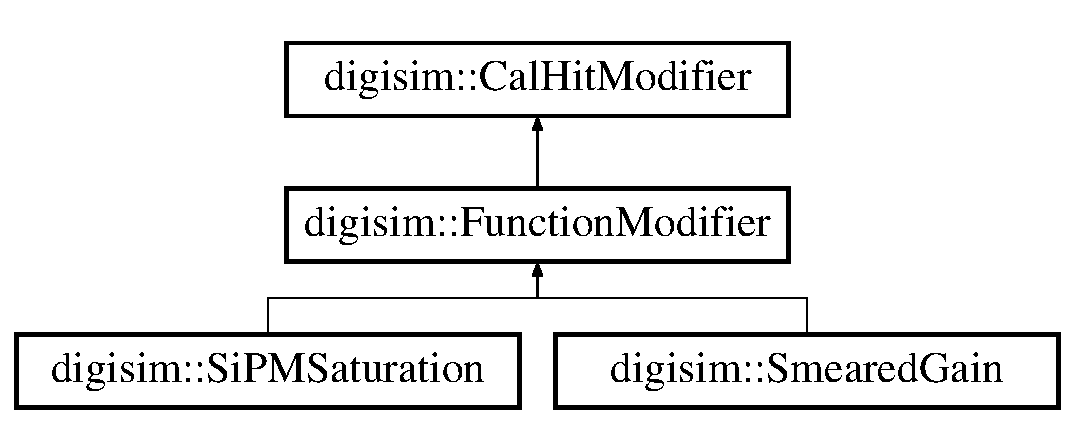
\includegraphics[height=3.000000cm]{classdigisim_1_1FunctionModifier}
\end{center}
\end{figure}
\subsection*{Public Member Functions}
\begin{DoxyCompactItemize}
\item 
virtual void {\bfseries init} (std\-::vector$<$ float $>$ \&floats)\label{classdigisim_1_1FunctionModifier_a096c2d2085e8ff8bc2f98de9af050332}

\item 
virtual void {\bfseries process\-Hits} (Temp\-Cal\-Hit\-Map \&hitmap)\label{classdigisim_1_1FunctionModifier_aaede6212f01bbb24472bdc7d30367d76}

\item 
virtual void {\bfseries print} () const \label{classdigisim_1_1FunctionModifier_a2a3a92b64b708286a4f37df6cbaece55}

\end{DoxyCompactItemize}
\subsection*{Protected Member Functions}
\begin{DoxyCompactItemize}
\item 
virtual double {\bfseries transform\-Energy} (const {\bf Temp\-Cal\-Hit} \&hit) const =0\label{classdigisim_1_1FunctionModifier_a6736a5a7ff1061b996e60f4363d9b4e4}

\item 
{\bfseries Function\-Modifier} (const std\-::string \&mod\-Name)\label{classdigisim_1_1FunctionModifier_a30e10898d170a7dec4cef34ebb1aca23}

\item 
{\bfseries Function\-Modifier} (const {\bf Function\-Modifier} \&rhs)\label{classdigisim_1_1FunctionModifier_a877cca17f351b27d1e1636b8c990f41b}

\end{DoxyCompactItemize}
\subsection*{Protected Attributes}
\begin{DoxyCompactItemize}
\item 
std\-::vector$<$ float $>$ {\bfseries \-\_\-par}\label{classdigisim_1_1FunctionModifier_a86987340330c332d2429614199bce001}

\end{DoxyCompactItemize}
\subsection*{Additional Inherited Members}


\subsection{Detailed Description}


Definition at line 19 of file Function\-Modifier.\-hpp.



The documentation for this class was generated from the following files\-:\begin{DoxyCompactItemize}
\item 
Function\-Modifier.\-hpp\item 
Function\-Modifier.\-cpp\end{DoxyCompactItemize}

\section{digisim\-:\-:Gain\-Discrimination Class Reference}
\label{classdigisim_1_1GainDiscrimination}\index{digisim\-::\-Gain\-Discrimination@{digisim\-::\-Gain\-Discrimination}}
Inheritance diagram for digisim\-:\-:Gain\-Discrimination\-:\begin{figure}[H]
\begin{center}
\leavevmode
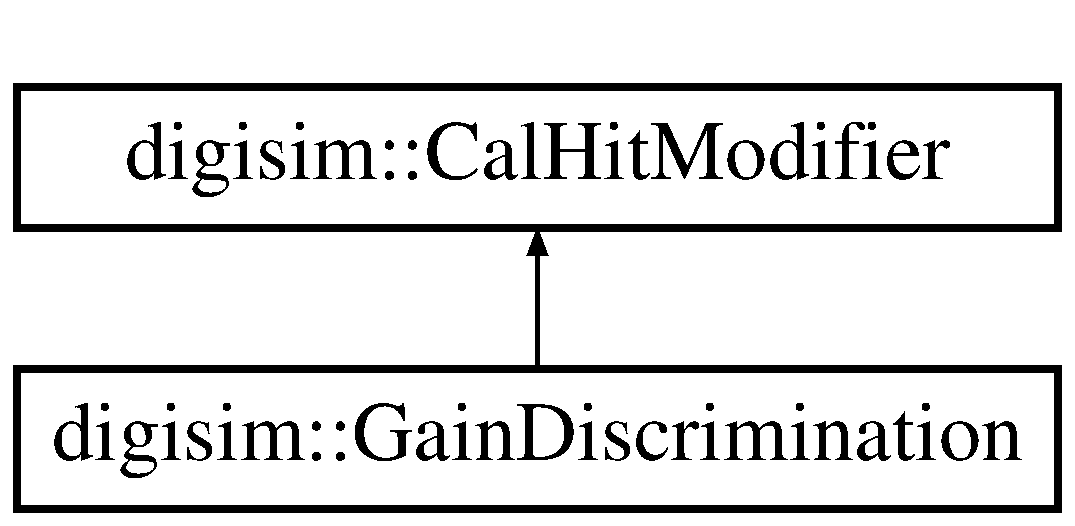
\includegraphics[height=2.000000cm]{classdigisim_1_1GainDiscrimination}
\end{center}
\end{figure}
\subsection*{Public Member Functions}
\begin{DoxyCompactItemize}
\item 
{\bf Gain\-Discrimination} $\ast$ {\bfseries new\-Instance} (const std\-::string \&mod\-Name)\label{classdigisim_1_1GainDiscrimination_aeda4bbdea05a86e08eccb75a86a371c4}

\item 
void {\bfseries init} (std\-::vector$<$ float $>$ \&floats)\label{classdigisim_1_1GainDiscrimination_a940ca3ec22fcafa4b878acb194ba8893}

\item 
void {\bfseries process\-Hits} (Temp\-Cal\-Hit\-Map \&hitmap)\label{classdigisim_1_1GainDiscrimination_a9a870bc250df2bb06ffed3f9307c89a9}

\item 
void {\bfseries print} () const \label{classdigisim_1_1GainDiscrimination_a72ef2d0767db5384296d4097a9614387}

\end{DoxyCompactItemize}
\subsection*{Private Member Functions}
\begin{DoxyCompactItemize}
\item 
{\bfseries Gain\-Discrimination} (const std\-::string \&mod\-Name)\label{classdigisim_1_1GainDiscrimination_abe382c5a7a32de7112b11698621d1245}

\item 
{\bfseries Gain\-Discrimination} (const {\bf Gain\-Discrimination} \&rhs)\label{classdigisim_1_1GainDiscrimination_a79702158c3183fecee7a6af2642be64b}

\item 
double {\bfseries energy\-To\-A\-D\-C} (const double ene)\label{classdigisim_1_1GainDiscrimination_ae2608651731ebb223b5485664b9e8376}

\item 
bool {\bfseries is\-Below\-Threshold} (const double adc)\label{classdigisim_1_1GainDiscrimination_a37f25c0a56cef0267c0b1add4c1da88d}

\end{DoxyCompactItemize}
\subsection*{Private Attributes}
\begin{DoxyCompactItemize}
\item 
std\-::vector$<$ float $>$ {\bfseries \-\_\-par}\label{classdigisim_1_1GainDiscrimination_a87163c1aaea57d296163d82f66d0f654}

\end{DoxyCompactItemize}
\subsection*{Additional Inherited Members}


\subsection{Detailed Description}


Definition at line 19 of file Gain\-Discrimination.\-hpp.



The documentation for this class was generated from the following files\-:\begin{DoxyCompactItemize}
\item 
Gain\-Discrimination.\-hpp\item 
Gain\-Discrimination.\-cpp\end{DoxyCompactItemize}

\section{C\-A\-L\-I\-C\-E\-:\-:Ganger Class Reference}
\label{classCALICE_1_1Ganger}\index{C\-A\-L\-I\-C\-E\-::\-Ganger@{C\-A\-L\-I\-C\-E\-::\-Ganger}}


The work horse.  




{\ttfamily \#include $<$Ahc2\-Ganging\-Processor.\-hh$>$}

Inheritance diagram for C\-A\-L\-I\-C\-E\-:\-:Ganger\-:\begin{figure}[H]
\begin{center}
\leavevmode
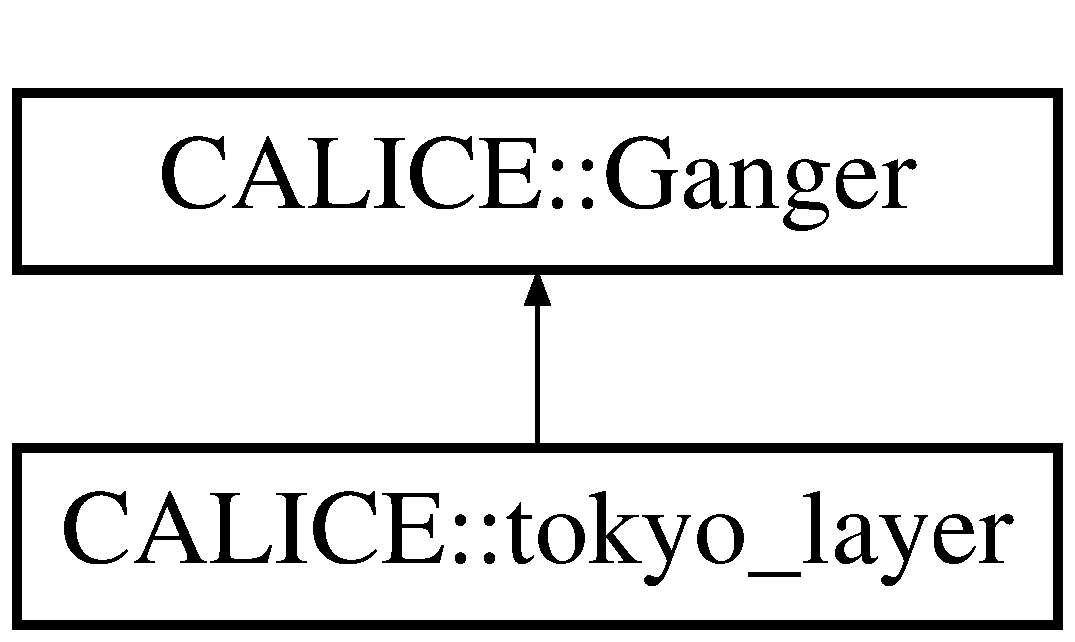
\includegraphics[height=2.000000cm]{classCALICE_1_1Ganger}
\end{center}
\end{figure}
\subsection*{Public Member Functions}
\begin{DoxyCompactItemize}
\item 
{\bf Ganger} (int cs, int off\-\_\-\-I, int off\-\_\-\-J, {\bf Contribution\-Map} $\ast$cm, float factor)\label{classCALICE_1_1Ganger_a314c60c0d692daed1d584ae5564d3928}

\begin{DoxyCompactList}\small\item\em The \doxyref{Ganger}{p.}{classCALICE_1_1Ganger} is constructed with all information needed for a region to perform the ganging. \end{DoxyCompactList}\item 
virtual bool {\bf responsible} ({\bf geometrical\-Indices} indices)=0\label{classCALICE_1_1Ganger_a57c5a2b853fec48755bfc12dd04ddfe8}

\begin{DoxyCompactList}\small\item\em Implementations have to implement where in I/\-J they are responsible. \end{DoxyCompactList}\item 
bool {\bf add\-Hit} ({\bf geometrical\-Indices} indices, Calorimeter\-Hit $\ast$hit)\label{classCALICE_1_1Ganger_a81b20222abc63c26b674ac9c7cefef0f}

\begin{DoxyCompactList}\small\item\em Function which return true if the ganger is responsible for this region and adds the hit to the Contribution\-Map. \end{DoxyCompactList}\item 
{\bf geometrical\-Indices} {\bf coarsen} ({\bf geometrical\-Indices} ijk)\label{classCALICE_1_1Ganger_ac7ca6e5fc4c8c7ffd45e6e03f7532b2a}

\begin{DoxyCompactList}\small\item\em Function which returns the ganged index according to the constants defined at construction. \end{DoxyCompactList}\item 
int {\bf coarsen\-Single\-Index} (int index, int offset)
\begin{DoxyCompactList}\small\item\em Performs mapping from Mokka indices to ganged indices. \end{DoxyCompactList}\end{DoxyCompactItemize}
\subsection*{Private Attributes}
\begin{DoxyCompactItemize}
\item 
int {\bf \-\_\-cell\-Size}\label{classCALICE_1_1Ganger_a815ccc10d250555de9ba6cc6af4f1765}

\begin{DoxyCompactList}\small\item\em Quadratic side length of the cells in the region the \doxyref{Ganger}{p.}{classCALICE_1_1Ganger} is responsible. \end{DoxyCompactList}\item 
int {\bf \-\_\-offset\-\_\-\-I}\label{classCALICE_1_1Ganger_a17e539b19b90e2c1104423fd157cde55}

\begin{DoxyCompactList}\small\item\em Offset with respect to starting counting at 1 for I. \end{DoxyCompactList}\item 
int {\bf \-\_\-offset\-\_\-\-J}\label{classCALICE_1_1Ganger_a721d1e57bd481872d8f39f2bd172c609}

\begin{DoxyCompactList}\small\item\em Offset with respect to starting counting at 1 for J. \end{DoxyCompactList}\item 
{\bf Contribution\-Map} $\ast$ {\bf \-\_\-contribution\-Map}\label{classCALICE_1_1Ganger_a653c4bbdb6e77cf562afba8c82a2dec9}

\begin{DoxyCompactList}\small\item\em Pointer to map which stores all ganged indices and Sim\-Calorimeter\-Hits. \end{DoxyCompactList}\item 
float {\bfseries \-\_\-tile\-Border\-Attenuation\-Factor}\label{classCALICE_1_1Ganger_a771cf6d407f49a4bf4b15d1fc1276b06}

\end{DoxyCompactItemize}


\subsection{Detailed Description}
The work horse. 

A ganger holds all information for a region to perform the ganging. 

Definition at line 119 of file Ahc2\-Ganging\-Processor.\-hh.



\subsection{Member Function Documentation}
\index{C\-A\-L\-I\-C\-E\-::\-Ganger@{C\-A\-L\-I\-C\-E\-::\-Ganger}!coarsen\-Single\-Index@{coarsen\-Single\-Index}}
\index{coarsen\-Single\-Index@{coarsen\-Single\-Index}!CALICE::Ganger@{C\-A\-L\-I\-C\-E\-::\-Ganger}}
\subsubsection[{coarsen\-Single\-Index}]{\setlength{\rightskip}{0pt plus 5cm}int C\-A\-L\-I\-C\-E\-::\-Ganger\-::coarsen\-Single\-Index (
\begin{DoxyParamCaption}
\item[{int}]{index, }
\item[{int}]{offset}
\end{DoxyParamCaption}
)\hspace{0.3cm}{\ttfamily [inline]}}\label{classCALICE_1_1Ganger_ae004d5984d63181208c71c7dbc347d0c}


Performs mapping from Mokka indices to ganged indices. 

The main \char`\"{}algorithm\char`\"{}. 

Definition at line 200 of file Ahc2\-Ganging\-Processor.\-hh.



The documentation for this class was generated from the following file\-:\begin{DoxyCompactItemize}
\item 
Ahc2\-Ganging\-Processor.\-hh\end{DoxyCompactItemize}

\section{C\-A\-L\-I\-C\-E\-:\-:A\-H\-C\-A\-L\-:\-:Digitization\-:\-:Ganging\-:\-:Ganger Class Reference}
\label{classCALICE_1_1AHCAL_1_1Digitization_1_1Ganging_1_1Ganger}\index{C\-A\-L\-I\-C\-E\-::\-A\-H\-C\-A\-L\-::\-Digitization\-::\-Ganging\-::\-Ganger@{C\-A\-L\-I\-C\-E\-::\-A\-H\-C\-A\-L\-::\-Digitization\-::\-Ganging\-::\-Ganger}}


The work horse.  




{\ttfamily \#include $<$ahcal\-Ganging\-Processor.\-hh$>$}

Inheritance diagram for C\-A\-L\-I\-C\-E\-:\-:A\-H\-C\-A\-L\-:\-:Digitization\-:\-:Ganging\-:\-:Ganger\-:\begin{figure}[H]
\begin{center}
\leavevmode
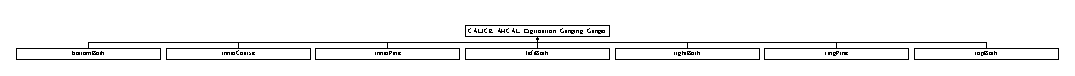
\includegraphics[height=0.567376cm]{classCALICE_1_1AHCAL_1_1Digitization_1_1Ganging_1_1Ganger}
\end{center}
\end{figure}
\subsection*{Public Member Functions}
\begin{DoxyCompactItemize}
\item 
{\bf Ganger} (int cs, int off\-\_\-\-I, int off\-\_\-\-J, {\bf Contribution\-Map} $\ast$cm, float factor)\label{classCALICE_1_1AHCAL_1_1Digitization_1_1Ganging_1_1Ganger_a3b7d24c593eb13aa8dae23e5931e936f}

\begin{DoxyCompactList}\small\item\em The \doxyref{Ganger}{p.}{classCALICE_1_1AHCAL_1_1Digitization_1_1Ganging_1_1Ganger} is constructed with all information needed for a region to perform the ganging. \end{DoxyCompactList}\item 
virtual bool {\bf responsible} ({\bf Geometrical\-Indices} indices)=0\label{classCALICE_1_1AHCAL_1_1Digitization_1_1Ganging_1_1Ganger_a58eb7020c646d0db74590858303eeeba}

\begin{DoxyCompactList}\small\item\em Implementations have to implement where in I/\-J they are responsible. \end{DoxyCompactList}\item 
bool {\bf add\-Hit} ({\bf Geometrical\-Indices} indices, Sim\-Calorimeter\-Hit $\ast$hit)\label{classCALICE_1_1AHCAL_1_1Digitization_1_1Ganging_1_1Ganger_a7024d60a5f237dc2db19e4c81c1e9a97}

\begin{DoxyCompactList}\small\item\em Function which return true if the ganger is responsible for this region and adds the hit to the Contribution\-Map. \end{DoxyCompactList}\item 
{\bf Geometrical\-Indices} {\bf coarsen} ({\bf Geometrical\-Indices} ijk)\label{classCALICE_1_1AHCAL_1_1Digitization_1_1Ganging_1_1Ganger_afffd6268f8c1458531747fa482981cdc}

\begin{DoxyCompactList}\small\item\em Function which returns the ganged index according to the constants defined at construction. \end{DoxyCompactList}\item 
int {\bf coarsen\-Single\-Index} (int index, int offset)
\begin{DoxyCompactList}\small\item\em Performs mapping from Mokka indices to ganged indices. \end{DoxyCompactList}\end{DoxyCompactItemize}
\subsection*{Private Attributes}
\begin{DoxyCompactItemize}
\item 
int {\bf \-\_\-cell\-Size}\label{classCALICE_1_1AHCAL_1_1Digitization_1_1Ganging_1_1Ganger_a2ffe3ad34f1abfb9d110ce3fbf4bae65}

\begin{DoxyCompactList}\small\item\em Quadratic side length of the cells in the region the \doxyref{Ganger}{p.}{classCALICE_1_1AHCAL_1_1Digitization_1_1Ganging_1_1Ganger} is responsible. \end{DoxyCompactList}\item 
int {\bf \-\_\-offset\-\_\-\-I}\label{classCALICE_1_1AHCAL_1_1Digitization_1_1Ganging_1_1Ganger_a1630400f2a2850426c19c523661d9a21}

\begin{DoxyCompactList}\small\item\em Offset with respect to starting counting at 1 for I. \end{DoxyCompactList}\item 
int {\bf \-\_\-offset\-\_\-\-J}\label{classCALICE_1_1AHCAL_1_1Digitization_1_1Ganging_1_1Ganger_a9699cfc25ea1267db7642c59b87e48e3}

\begin{DoxyCompactList}\small\item\em Offset with respect to starting counting at 1 for J. \end{DoxyCompactList}\item 
{\bf Contribution\-Map} $\ast$ {\bf \-\_\-\-C\-M}\label{classCALICE_1_1AHCAL_1_1Digitization_1_1Ganging_1_1Ganger_a46c0222468c6e579e36aa02d04064518}

\begin{DoxyCompactList}\small\item\em Pointer to map which stores all ganged indices and Sim\-Calorimeter\-Hits. \end{DoxyCompactList}\item 
float {\bfseries \-\_\-tile\-Border\-Attenuation\-Factor}\label{classCALICE_1_1AHCAL_1_1Digitization_1_1Ganging_1_1Ganger_a4e6dad3dc780014323f79f0fa2390fe1}

\end{DoxyCompactItemize}


\subsection{Detailed Description}
The work horse. 

A ganger holds all information for a region to perform the ganging. 

Definition at line 145 of file ahcal\-Ganging\-Processor.\-hh.



\subsection{Member Function Documentation}
\index{C\-A\-L\-I\-C\-E\-::\-A\-H\-C\-A\-L\-::\-Digitization\-::\-Ganging\-::\-Ganger@{C\-A\-L\-I\-C\-E\-::\-A\-H\-C\-A\-L\-::\-Digitization\-::\-Ganging\-::\-Ganger}!coarsen\-Single\-Index@{coarsen\-Single\-Index}}
\index{coarsen\-Single\-Index@{coarsen\-Single\-Index}!CALICE::AHCAL::Digitization::Ganging::Ganger@{C\-A\-L\-I\-C\-E\-::\-A\-H\-C\-A\-L\-::\-Digitization\-::\-Ganging\-::\-Ganger}}
\subsubsection[{coarsen\-Single\-Index}]{\setlength{\rightskip}{0pt plus 5cm}int C\-A\-L\-I\-C\-E\-::\-A\-H\-C\-A\-L\-::\-Digitization\-::\-Ganging\-::\-Ganger\-::coarsen\-Single\-Index (
\begin{DoxyParamCaption}
\item[{int}]{index, }
\item[{int}]{offset}
\end{DoxyParamCaption}
)\hspace{0.3cm}{\ttfamily [inline]}}\label{classCALICE_1_1AHCAL_1_1Digitization_1_1Ganging_1_1Ganger_a3b7c7319137acba5afc98ce3be336281}


Performs mapping from Mokka indices to ganged indices. 

The main \char`\"{}algorithm\char`\"{}. 

Definition at line 241 of file ahcal\-Ganging\-Processor.\-hh.



References \-\_\-cell\-Size.



Referenced by coarsen().



The documentation for this class was generated from the following file\-:\begin{DoxyCompactItemize}
\item 
ahcal\-Ganging\-Processor.\-hh\end{DoxyCompactItemize}

\section{C\-A\-L\-I\-C\-E\-:\-:geometrical\-Indices Struct Reference}
\label{structCALICE_1_1geometricalIndices}\index{C\-A\-L\-I\-C\-E\-::geometrical\-Indices@{C\-A\-L\-I\-C\-E\-::geometrical\-Indices}}


Helper class to store I, J, K.  




{\ttfamily \#include $<$Ahc2\-Ganging\-Processor.\-hh$>$}

\subsection*{Data Fields}
\begin{DoxyCompactItemize}
\item 
int {\bfseries I}\label{structCALICE_1_1geometricalIndices_a169eb9cf47d6ad4dc508e712e7a39ee9}

\item 
int {\bfseries J}\label{structCALICE_1_1geometricalIndices_a0dd42ea7ba3919a89f2ffcb8f81010a7}

\item 
int {\bfseries K}\label{structCALICE_1_1geometricalIndices_ab61a6aed9ef9f3aa82f0cb971386a2aa}

\end{DoxyCompactItemize}


\subsection{Detailed Description}
Helper class to store I, J, K. 

Definition at line 28 of file Ahc2\-Ganging\-Processor.\-hh.



The documentation for this struct was generated from the following file\-:\begin{DoxyCompactItemize}
\item 
Ahc2\-Ganging\-Processor.\-hh\end{DoxyCompactItemize}

\section{C\-A\-L\-I\-C\-E\-:\-:A\-H\-C\-A\-L\-:\-:Digitization\-:\-:Ganging\-:\-:Geometrical\-Indices Struct Reference}
\label{structCALICE_1_1AHCAL_1_1Digitization_1_1Ganging_1_1GeometricalIndices}\index{C\-A\-L\-I\-C\-E\-::\-A\-H\-C\-A\-L\-::\-Digitization\-::\-Ganging\-::\-Geometrical\-Indices@{C\-A\-L\-I\-C\-E\-::\-A\-H\-C\-A\-L\-::\-Digitization\-::\-Ganging\-::\-Geometrical\-Indices}}


Helper class to store I, J, K.  




{\ttfamily \#include $<$ahcal\-Ganging\-Processor.\-hh$>$}

\subsection*{Data Fields}
\begin{DoxyCompactItemize}
\item 
int {\bfseries I}\label{structCALICE_1_1AHCAL_1_1Digitization_1_1Ganging_1_1GeometricalIndices_a00ea48769a635791267befbaafc7c108}

\item 
int {\bfseries J}\label{structCALICE_1_1AHCAL_1_1Digitization_1_1Ganging_1_1GeometricalIndices_a1aea854b7760847766a913eb21ee92b6}

\item 
int {\bfseries K}\label{structCALICE_1_1AHCAL_1_1Digitization_1_1Ganging_1_1GeometricalIndices_adc1fe191a35572a32d77db4b69d1e4e5}

\end{DoxyCompactItemize}


\subsection{Detailed Description}
Helper class to store I, J, K. 

Definition at line 24 of file ahcal\-Ganging\-Processor.\-hh.



The documentation for this struct was generated from the following file\-:\begin{DoxyCompactItemize}
\item 
ahcal\-Ganging\-Processor.\-hh\end{DoxyCompactItemize}

\section{digisim\-:\-:Hit\-Contrib Class Reference}
\label{classdigisim_1_1HitContrib}\index{digisim\-::\-Hit\-Contrib@{digisim\-::\-Hit\-Contrib}}
\subsection*{Public Member Functions}
\begin{DoxyCompactItemize}
\item 
{\bfseries Hit\-Contrib} (double energy, double time)\label{classdigisim_1_1HitContrib_a7244bc624861aa524c78e73cf7e0aba8}

\item 
double {\bfseries energy} () const \label{classdigisim_1_1HitContrib_a62ccf479e2c6f9066b0a53fc3dc87db2}

\item 
double {\bfseries time} () const \label{classdigisim_1_1HitContrib_af7da03bdadde1b872b26d843ece7d077}

\item 
void {\bfseries scale} (double factor)\label{classdigisim_1_1HitContrib_a934eee555d6d93abd79cb945307e78a4}

\item 
void {\bfseries increment} (double energy, double time)\label{classdigisim_1_1HitContrib_a0d9be0f90a021e9d6f979d9d2c2b48d4}

\end{DoxyCompactItemize}
\subsection*{Private Attributes}
\begin{DoxyCompactItemize}
\item 
double {\bfseries \-\_\-energy}\label{classdigisim_1_1HitContrib_aaf384d2e5576cfa2c6f90b862da13023}

\item 
double {\bfseries \-\_\-time}\label{classdigisim_1_1HitContrib_a98d7fc48134364bb4a2e8ebc2d603eed}

\end{DoxyCompactItemize}


\subsection{Detailed Description}


Definition at line 6 of file Hit\-Contrib.\-hpp.



The documentation for this class was generated from the following files\-:\begin{DoxyCompactItemize}
\item 
Hit\-Contrib.\-hpp\item 
Hit\-Contrib.\-cpp\end{DoxyCompactItemize}

\section{inner\-Coarse Class Reference}
\label{classinnerCoarse}\index{inner\-Coarse@{inner\-Coarse}}


Implementation of ganger.  


Inheritance diagram for inner\-Coarse\-:\begin{figure}[H]
\begin{center}
\leavevmode
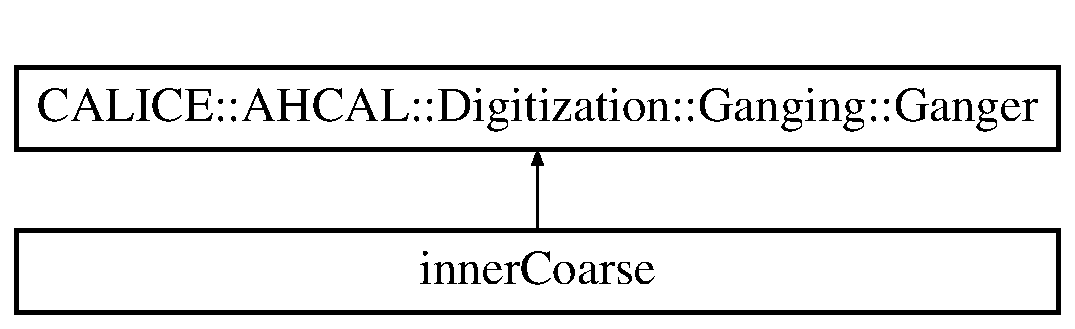
\includegraphics[height=2.000000cm]{classinnerCoarse}
\end{center}
\end{figure}
\subsection*{Public Member Functions}
\begin{DoxyCompactItemize}
\item 
{\bfseries inner\-Coarse} ({\bf Contribution\-Map} $\ast$cm, float factor)\label{classinnerCoarse_a4273c4497fb348c311677291af0940b2}

\item 
bool {\bf responsible} ({\bf Geometrical\-Indices} indices)\label{classinnerCoarse_a35f969c20bf726dacc6a06a1bef2030e}

\begin{DoxyCompactList}\small\item\em Implementations have to implement where in I/\-J they are responsible. \end{DoxyCompactList}\end{DoxyCompactItemize}


\subsection{Detailed Description}
Implementation of ganger. 

Definition at line 83 of file ahcal\-Ganging\-Processor.\-cc.



The documentation for this class was generated from the following file\-:\begin{DoxyCompactItemize}
\item 
ahcal\-Ganging\-Processor.\-cc\end{DoxyCompactItemize}

\section{inner\-Fine Class Reference}
\label{classinnerFine}\index{inner\-Fine@{inner\-Fine}}


Implementation of ganger.  


Inheritance diagram for inner\-Fine\-:\begin{figure}[H]
\begin{center}
\leavevmode
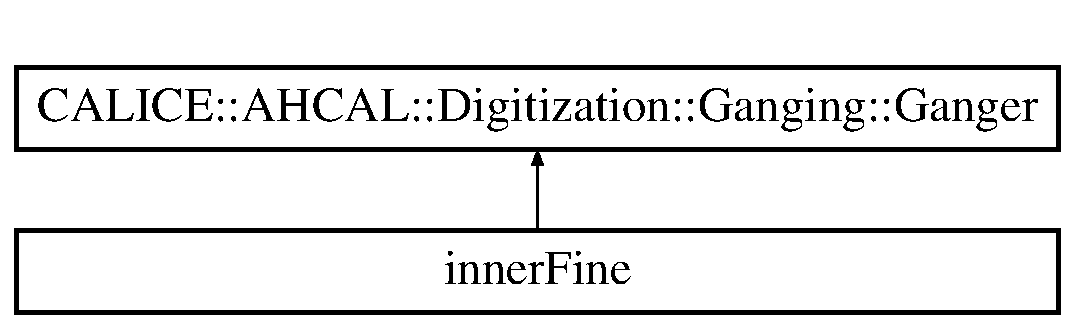
\includegraphics[height=2.000000cm]{classinnerFine}
\end{center}
\end{figure}
\subsection*{Public Member Functions}
\begin{DoxyCompactItemize}
\item 
{\bfseries inner\-Fine} ({\bf Contribution\-Map} $\ast$cm, float factor)\label{classinnerFine_a9c0cef5d4f92b6f0355ea85f5ec30df5}

\item 
bool {\bf responsible} ({\bf Geometrical\-Indices} indices)\label{classinnerFine_a4e260cbea93dfdbeb8cdd524b2fc6609}

\begin{DoxyCompactList}\small\item\em Implementations have to implement where in I/\-J they are responsible. \end{DoxyCompactList}\end{DoxyCompactItemize}


\subsection{Detailed Description}
Implementation of ganger. 

Definition at line 44 of file ahcal\-Ganging\-Processor.\-cc.



The documentation for this class was generated from the following file\-:\begin{DoxyCompactItemize}
\item 
ahcal\-Ganging\-Processor.\-cc\end{DoxyCompactItemize}

\section{C\-A\-L\-I\-C\-E\-:\-:A\-H\-C\-A\-L\-:\-:Digitization\-:\-:Integrated\-Hcal\-Digitization\-Processor Class Reference}
\label{classCALICE_1_1AHCAL_1_1Digitization_1_1IntegratedHcalDigitizationProcessor}\index{C\-A\-L\-I\-C\-E\-::\-A\-H\-C\-A\-L\-::\-Digitization\-::\-Integrated\-Hcal\-Digitization\-Processor@{C\-A\-L\-I\-C\-E\-::\-A\-H\-C\-A\-L\-::\-Digitization\-::\-Integrated\-Hcal\-Digitization\-Processor}}


Processor to digitized Monte Carlo hits.  




{\ttfamily \#include $<$Integrated\-Hcal\-Digitization\-Processor.\-hh$>$}

Inheritance diagram for C\-A\-L\-I\-C\-E\-:\-:A\-H\-C\-A\-L\-:\-:Digitization\-:\-:Integrated\-Hcal\-Digitization\-Processor\-:\begin{figure}[H]
\begin{center}
\leavevmode
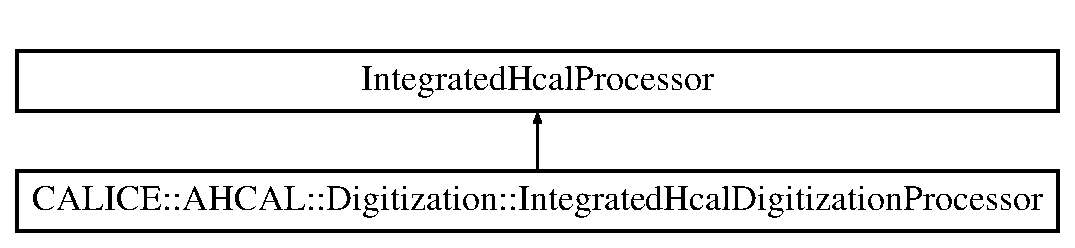
\includegraphics[height=2.000000cm]{classCALICE_1_1AHCAL_1_1Digitization_1_1IntegratedHcalDigitizationProcessor}
\end{center}
\end{figure}
\subsection*{Public Member Functions}
\begin{DoxyCompactItemize}
\item 
{\bf Integrated\-Hcal\-Digitization\-Processor} $\ast$ {\bfseries new\-Processor} ()\label{classCALICE_1_1AHCAL_1_1Digitization_1_1IntegratedHcalDigitizationProcessor_a4109708387041804b890e38fa84a4528}

\item 
void {\bf init} ()
\begin{DoxyCompactList}\small\item\em Everything which has to be initialized once before the processing of the events can start goes here. \end{DoxyCompactList}\item 
void {\bf process\-Event} (lcio\-::\-L\-C\-Event $\ast$evt)
\begin{DoxyCompactList}\small\item\em This function is called for every event if the Digitization\-Processor is active. \end{DoxyCompactList}\item 
void {\bf end} ()
\begin{DoxyCompactList}\small\item\em At the very end of Marlin this function is called. \end{DoxyCompactList}\end{DoxyCompactItemize}
\subsection*{Private Member Functions}
\begin{DoxyCompactItemize}
\item 
void {\bf init\-Random\-Generator} ()\label{classCALICE_1_1AHCAL_1_1Digitization_1_1IntegratedHcalDigitizationProcessor_a2db3f59f163c013fb32a9e51f0c3e9f1}

\begin{DoxyCompactList}\small\item\em Initialization of the random generator for pixel statistic simulation. \end{DoxyCompactList}\item 
void {\bf open\-Input\-Collections} (lcio\-::\-L\-C\-Event $\ast$evt)
\begin{DoxyCompactList}\small\item\em Open the input collections\-: incoming Sim\-Calorimeter\-Hits and noise. \end{DoxyCompactList}\item 
void {\bf simulate\-Optical\-Crosstalk} ()\label{classCALICE_1_1AHCAL_1_1Digitization_1_1IntegratedHcalDigitizationProcessor_ab412228819b6143acbde9e0ddec1303f}

\begin{DoxyCompactList}\small\item\em Hits are copied to a temporary map and optical crosstalk is simulated. \end{DoxyCompactList}\item 
void {\bf simulate\-Si\-P\-M\-Behaviour} ()\label{classCALICE_1_1AHCAL_1_1Digitization_1_1IntegratedHcalDigitizationProcessor_a41c3b67f6c7c61a7cf630f0ad59a6d67}

\begin{DoxyCompactList}\small\item\em In this function saturation and pixel statistic are simulated. \end{DoxyCompactList}\item 
void {\bf merge\-Hits\-And\-Noise} ()\label{classCALICE_1_1AHCAL_1_1Digitization_1_1IntegratedHcalDigitizationProcessor_a29bab9438d4502f55b4239d0b1da490d}

\begin{DoxyCompactList}\small\item\em The digitized event is add on top of the noise event. \end{DoxyCompactList}\item 
void {\bf create\-Output\-Collections} (lcio\-::\-L\-C\-Event $\ast$evt)\label{classCALICE_1_1AHCAL_1_1Digitization_1_1IntegratedHcalDigitizationProcessor_a6f0fb41bf2db27149a40d87e38568637}

\begin{DoxyCompactList}\small\item\em Create the digitized + noise collection. \end{DoxyCompactList}\item 
void {\bf tidy\-Up} ()\label{classCALICE_1_1AHCAL_1_1Digitization_1_1IntegratedHcalDigitizationProcessor_ab11f8e3070251f8b2441a891c2094d62}

\begin{DoxyCompactList}\small\item\em Resets everything which is event specific. \end{DoxyCompactList}\item 
double {\bf get\-Cell\-Size} (int module, int chip, int channel)
\begin{DoxyCompactList}\small\item\em from Integrated\-Hcal\-Processor, Si\-P\-M\-Properties\-Processor \end{DoxyCompactList}\end{DoxyCompactItemize}
\subsection*{Private Attributes}
\begin{DoxyCompactItemize}
\item 
std\-::string {\bf \-\_\-input\-Col\-Name}\label{classCALICE_1_1AHCAL_1_1Digitization_1_1IntegratedHcalDigitizationProcessor_ae06b4559fe0be19b6821dd09c0e4ba61}

\begin{DoxyCompactList}\small\item\em Name of the ganged collection which will be digitized. \end{DoxyCompactList}\item 
std\-::string {\bf \-\_\-noise\-Col\-Name}\label{classCALICE_1_1AHCAL_1_1Digitization_1_1IntegratedHcalDigitizationProcessor_a2ef49e103b2c5b84daf7932e20a92a0e}

\begin{DoxyCompactList}\small\item\em Name of the noise collection which will be overlayed. \end{DoxyCompactList}\item 
std\-::string {\bf \-\_\-output\-Col\-Name}
\begin{DoxyCompactList}\small\item\em Name of the digitized collection. \end{DoxyCompactList}\item 
Neighbour\-Relations\-::\-Fine\-Module {\bf \-\_\-a\-Fine\-Module}\label{classCALICE_1_1AHCAL_1_1Digitization_1_1IntegratedHcalDigitizationProcessor_a53e7c1a392534c468c52b5362c9a3040}

\begin{DoxyCompactList}\small\item\em Instance which can be asked about neighbour relations of a fine module. \end{DoxyCompactList}\item 
Neighbour\-Relations\-::\-Coarse\-Module {\bf \-\_\-a\-Coarse\-Module}\label{classCALICE_1_1AHCAL_1_1Digitization_1_1IntegratedHcalDigitizationProcessor_ab1b07e4084157a8e75568179afd78cea}

\begin{DoxyCompactList}\small\item\em Instance which can be asked about neighbour relations of a fine module. \end{DoxyCompactList}\item 
lcio\-::\-Cell\-I\-D\-Decoder\\*
$<$ lcio\-::\-Calorimeter\-Hit $>$ $\ast$ {\bf \-\_\-p\-Incoming\-Cell\-I\-D\-Decoder}\label{classCALICE_1_1AHCAL_1_1Digitization_1_1IntegratedHcalDigitizationProcessor_abd1eedcf23d9def06b38f1aa89cf555c}

\begin{DoxyCompactList}\small\item\em To have he \doxyref{Cell\-I\-D\-Decoder}{p.}{classCellIDDecoder} available in every member function we hold a pointer of it. \end{DoxyCompactList}\item 
lcio\-::\-Cell\-I\-D\-Encoder\\*
$<$ lcio\-::\-Calorimeter\-Hit\-Impl $>$ $\ast$ {\bf \-\_\-p\-Outgoing\-Cell\-I\-D\-Encoder}\label{classCALICE_1_1AHCAL_1_1Digitization_1_1IntegratedHcalDigitizationProcessor_a4bd23776f39b61fb851e56c2e1af7c21}

\begin{DoxyCompactList}\small\item\em To have he Cell\-I\-D\-Encoder available in every member function we hold a pointer of it. \end{DoxyCompactList}\item 
lcio\-::\-L\-C\-Collection $\ast$ {\bf \-\_\-ganged\-M\-C\-Col}\label{classCALICE_1_1AHCAL_1_1Digitization_1_1IntegratedHcalDigitizationProcessor_a2eca1d5b8899e69dd6653732601dfca7}

\begin{DoxyCompactList}\small\item\em Pointer to the incoming collection. \end{DoxyCompactList}\item 
lcio\-::\-L\-C\-Collection $\ast$ {\bf \-\_\-noise\-Col}\label{classCALICE_1_1AHCAL_1_1Digitization_1_1IntegratedHcalDigitizationProcessor_aa40cc79bbf8ee331059d6ee02db1c131}

\begin{DoxyCompactList}\small\item\em Pointer to the noise collection. \end{DoxyCompactList}\item 
float {\bf \-\_\-leakage}
\begin{DoxyCompactList}\small\item\em Factor of optical crosstalk/leakage. \end{DoxyCompactList}\item 
float {\bf \-\_\-mip\-Ge\-V}
\begin{DoxyCompactList}\small\item\em Energy per M\-I\-P. \end{DoxyCompactList}\item 
T\-Random3 $\ast$ {\bf \-\_\-p\-Random\-Generator}\label{classCALICE_1_1AHCAL_1_1Digitization_1_1IntegratedHcalDigitizationProcessor_af9a0090b772ecce3a2b38d593111a0c8}

\begin{DoxyCompactList}\small\item\em Pointer to R\-O\-O\-Ts random generator for pixel statistics. \end{DoxyCompactList}\item 
int {\bf \-\_\-random\-Seed}
\begin{DoxyCompactList}\small\item\em The random seed for the random generator. \end{DoxyCompactList}\item 
std\-::map$<$ int, double $>$ {\bf \-\_\-hcal\-Tile\-Index\-To\-Amplitude}
\begin{DoxyCompactList}\small\item\em The main map. \end{DoxyCompactList}\item 
bool {\bf \-\_\-do\-Stat}\label{classCALICE_1_1AHCAL_1_1Digitization_1_1IntegratedHcalDigitizationProcessor_a2db3e5df11e5ef9627efe1228424074b}

\begin{DoxyCompactList}\small\item\em Toggle to simulate pixel statistics. \end{DoxyCompactList}\end{DoxyCompactItemize}


\subsection{Detailed Description}
Processor to digitized Monte Carlo hits. 

This Digitization\-Processor converts the energy deposition per cell to hardware units while simulating various detector effects like\-: optical crosstalk, pixel statistic, saturation and noise.

\begin{DoxyAuthor}{Authors}
Sebastian Richter 
\end{DoxyAuthor}
\begin{DoxyVersion}{Version}
1.\-0 
\end{DoxyVersion}


Definition at line 53 of file Integrated\-Hcal\-Digitization\-Processor.\-hh.



\subsection{Member Function Documentation}
\index{C\-A\-L\-I\-C\-E\-::\-A\-H\-C\-A\-L\-::\-Digitization\-::\-Integrated\-Hcal\-Digitization\-Processor@{C\-A\-L\-I\-C\-E\-::\-A\-H\-C\-A\-L\-::\-Digitization\-::\-Integrated\-Hcal\-Digitization\-Processor}!end@{end}}
\index{end@{end}!CALICE::AHCAL::Digitization::IntegratedHcalDigitizationProcessor@{C\-A\-L\-I\-C\-E\-::\-A\-H\-C\-A\-L\-::\-Digitization\-::\-Integrated\-Hcal\-Digitization\-Processor}}
\subsubsection[{end}]{\setlength{\rightskip}{0pt plus 5cm}void Integrated\-Hcal\-Digitization\-Processor\-::end (
\begin{DoxyParamCaption}
{}
\end{DoxyParamCaption}
)}\label{classCALICE_1_1AHCAL_1_1Digitization_1_1IntegratedHcalDigitizationProcessor_a7107bda788bc2a48b67bb1999f501bb3}


At the very end of Marlin this function is called. 

Think of it as the reverse of \doxyref{init()}{p.}{classCALICE_1_1AHCAL_1_1Digitization_1_1IntegratedHcalDigitizationProcessor_ab6ea84a6486d90ea84b0c41c14ef1de5}. Delete newed objects. 

Definition at line 505 of file Integrated\-Hcal\-Digitization\-Processor.\-cc.

\index{C\-A\-L\-I\-C\-E\-::\-A\-H\-C\-A\-L\-::\-Digitization\-::\-Integrated\-Hcal\-Digitization\-Processor@{C\-A\-L\-I\-C\-E\-::\-A\-H\-C\-A\-L\-::\-Digitization\-::\-Integrated\-Hcal\-Digitization\-Processor}!get\-Cell\-Size@{get\-Cell\-Size}}
\index{get\-Cell\-Size@{get\-Cell\-Size}!CALICE::AHCAL::Digitization::IntegratedHcalDigitizationProcessor@{C\-A\-L\-I\-C\-E\-::\-A\-H\-C\-A\-L\-::\-Digitization\-::\-Integrated\-Hcal\-Digitization\-Processor}}
\subsubsection[{get\-Cell\-Size}]{\setlength{\rightskip}{0pt plus 5cm}double C\-A\-L\-I\-C\-E\-::\-A\-H\-C\-A\-L\-::\-Digitization\-::\-Integrated\-Hcal\-Digitization\-Processor\-::get\-Cell\-Size (
\begin{DoxyParamCaption}
\item[{int}]{module, }
\item[{int}]{chip, }
\item[{int}]{channel}
\end{DoxyParamCaption}
)\hspace{0.3cm}{\ttfamily [inline]}, {\ttfamily [private]}}\label{classCALICE_1_1AHCAL_1_1Digitization_1_1IntegratedHcalDigitizationProcessor_aad3abb59471ecda56973de80d84b5780}


from Integrated\-Hcal\-Processor, Si\-P\-M\-Properties\-Processor 

from Integrated\-Hcal\-Processor, Si\-P\-M\-Properties\-Processor 

Definition at line 155 of file Integrated\-Hcal\-Digitization\-Processor.\-hh.

\index{C\-A\-L\-I\-C\-E\-::\-A\-H\-C\-A\-L\-::\-Digitization\-::\-Integrated\-Hcal\-Digitization\-Processor@{C\-A\-L\-I\-C\-E\-::\-A\-H\-C\-A\-L\-::\-Digitization\-::\-Integrated\-Hcal\-Digitization\-Processor}!init@{init}}
\index{init@{init}!CALICE::AHCAL::Digitization::IntegratedHcalDigitizationProcessor@{C\-A\-L\-I\-C\-E\-::\-A\-H\-C\-A\-L\-::\-Digitization\-::\-Integrated\-Hcal\-Digitization\-Processor}}
\subsubsection[{init}]{\setlength{\rightskip}{0pt plus 5cm}void Integrated\-Hcal\-Digitization\-Processor\-::init (
\begin{DoxyParamCaption}
{}
\end{DoxyParamCaption}
)}\label{classCALICE_1_1AHCAL_1_1Digitization_1_1IntegratedHcalDigitizationProcessor_ab6ea84a6486d90ea84b0c41c14ef1de5}


Everything which has to be initialized once before the processing of the events can start goes here. 

The init of the base class processor (Integrated\-Hcal\-Processor) is called (never forget it!).

A random generator is set up\-: \doxyref{init\-Random\-Generator()}{p.}{classCALICE_1_1AHCAL_1_1Digitization_1_1IntegratedHcalDigitizationProcessor_a2db3f59f163c013fb32a9e51f0c3e9f1} 

Definition at line 69 of file Integrated\-Hcal\-Digitization\-Processor.\-cc.

\index{C\-A\-L\-I\-C\-E\-::\-A\-H\-C\-A\-L\-::\-Digitization\-::\-Integrated\-Hcal\-Digitization\-Processor@{C\-A\-L\-I\-C\-E\-::\-A\-H\-C\-A\-L\-::\-Digitization\-::\-Integrated\-Hcal\-Digitization\-Processor}!open\-Input\-Collections@{open\-Input\-Collections}}
\index{open\-Input\-Collections@{open\-Input\-Collections}!CALICE::AHCAL::Digitization::IntegratedHcalDigitizationProcessor@{C\-A\-L\-I\-C\-E\-::\-A\-H\-C\-A\-L\-::\-Digitization\-::\-Integrated\-Hcal\-Digitization\-Processor}}
\subsubsection[{open\-Input\-Collections}]{\setlength{\rightskip}{0pt plus 5cm}void Integrated\-Hcal\-Digitization\-Processor\-::open\-Input\-Collections (
\begin{DoxyParamCaption}
\item[{lcio\-::\-L\-C\-Event $\ast$}]{evt}
\end{DoxyParamCaption}
)\hspace{0.3cm}{\ttfamily [private]}}\label{classCALICE_1_1AHCAL_1_1Digitization_1_1IntegratedHcalDigitizationProcessor_a69cae8f7f9de82e98d65a7fe5e87afac}


Open the input collections\-: incoming Sim\-Calorimeter\-Hits and noise. 



Definition at line 127 of file Integrated\-Hcal\-Digitization\-Processor.\-cc.

\index{C\-A\-L\-I\-C\-E\-::\-A\-H\-C\-A\-L\-::\-Digitization\-::\-Integrated\-Hcal\-Digitization\-Processor@{C\-A\-L\-I\-C\-E\-::\-A\-H\-C\-A\-L\-::\-Digitization\-::\-Integrated\-Hcal\-Digitization\-Processor}!process\-Event@{process\-Event}}
\index{process\-Event@{process\-Event}!CALICE::AHCAL::Digitization::IntegratedHcalDigitizationProcessor@{C\-A\-L\-I\-C\-E\-::\-A\-H\-C\-A\-L\-::\-Digitization\-::\-Integrated\-Hcal\-Digitization\-Processor}}
\subsubsection[{process\-Event}]{\setlength{\rightskip}{0pt plus 5cm}void Integrated\-Hcal\-Digitization\-Processor\-::process\-Event (
\begin{DoxyParamCaption}
\item[{lcio\-::\-L\-C\-Event $\ast$}]{evt}
\end{DoxyParamCaption}
)}\label{classCALICE_1_1AHCAL_1_1Digitization_1_1IntegratedHcalDigitizationProcessor_afa77031d626abc734f01bc1518a12d85}


This function is called for every event if the Digitization\-Processor is active. 

It starts a couple of functions like\-:

\begin{DoxyItemize}
\item \doxyref{open\-Input\-Collections()}{p.}{classCALICE_1_1AHCAL_1_1Digitization_1_1IntegratedHcalDigitizationProcessor_a69cae8f7f9de82e98d65a7fe5e87afac} \item \doxyref{simulate\-Optical\-Crosstalk()}{p.}{classCALICE_1_1AHCAL_1_1Digitization_1_1IntegratedHcalDigitizationProcessor_ab412228819b6143acbde9e0ddec1303f} \item \doxyref{simulate\-Si\-P\-M\-Behaviour()}{p.}{classCALICE_1_1AHCAL_1_1Digitization_1_1IntegratedHcalDigitizationProcessor_a41c3b67f6c7c61a7cf630f0ad59a6d67} \item \doxyref{merge\-Hits\-And\-Noise()}{p.}{classCALICE_1_1AHCAL_1_1Digitization_1_1IntegratedHcalDigitizationProcessor_a29bab9438d4502f55b4239d0b1da490d} \item \doxyref{create\-Output\-Collections()}{p.}{classCALICE_1_1AHCAL_1_1Digitization_1_1IntegratedHcalDigitizationProcessor_a6f0fb41bf2db27149a40d87e38568637}\end{DoxyItemize}
and at the very end to clear all non-\/temperory maps etc.\-:

\begin{DoxyItemize}
\item \doxyref{tidy\-Up()}{p.}{classCALICE_1_1AHCAL_1_1Digitization_1_1IntegratedHcalDigitizationProcessor_ab11f8e3070251f8b2441a891c2094d62}\end{DoxyItemize}
If you want to know what's going on I suggest to go through all the functions in the given order. 

Definition at line 94 of file Integrated\-Hcal\-Digitization\-Processor.\-cc.



\subsection{Field Documentation}
\index{C\-A\-L\-I\-C\-E\-::\-A\-H\-C\-A\-L\-::\-Digitization\-::\-Integrated\-Hcal\-Digitization\-Processor@{C\-A\-L\-I\-C\-E\-::\-A\-H\-C\-A\-L\-::\-Digitization\-::\-Integrated\-Hcal\-Digitization\-Processor}!\-\_\-hcal\-Tile\-Index\-To\-Amplitude@{\-\_\-hcal\-Tile\-Index\-To\-Amplitude}}
\index{\-\_\-hcal\-Tile\-Index\-To\-Amplitude@{\-\_\-hcal\-Tile\-Index\-To\-Amplitude}!CALICE::AHCAL::Digitization::IntegratedHcalDigitizationProcessor@{C\-A\-L\-I\-C\-E\-::\-A\-H\-C\-A\-L\-::\-Digitization\-::\-Integrated\-Hcal\-Digitization\-Processor}}
\subsubsection[{\-\_\-hcal\-Tile\-Index\-To\-Amplitude}]{\setlength{\rightskip}{0pt plus 5cm}std\-::map$<$int,double$>$ C\-A\-L\-I\-C\-E\-::\-A\-H\-C\-A\-L\-::\-Digitization\-::\-Integrated\-Hcal\-Digitization\-Processor\-::\-\_\-hcal\-Tile\-Index\-To\-Amplitude\hspace{0.3cm}{\ttfamily [private]}}\label{classCALICE_1_1AHCAL_1_1Digitization_1_1IntegratedHcalDigitizationProcessor_ae4722af37984307f7481c1b1a2deecd4}


The main map. 

This holds the current amplitude. For performance its unit change during each step of digitization. 

Definition at line 220 of file Integrated\-Hcal\-Digitization\-Processor.\-hh.

\index{C\-A\-L\-I\-C\-E\-::\-A\-H\-C\-A\-L\-::\-Digitization\-::\-Integrated\-Hcal\-Digitization\-Processor@{C\-A\-L\-I\-C\-E\-::\-A\-H\-C\-A\-L\-::\-Digitization\-::\-Integrated\-Hcal\-Digitization\-Processor}!\-\_\-leakage@{\-\_\-leakage}}
\index{\-\_\-leakage@{\-\_\-leakage}!CALICE::AHCAL::Digitization::IntegratedHcalDigitizationProcessor@{C\-A\-L\-I\-C\-E\-::\-A\-H\-C\-A\-L\-::\-Digitization\-::\-Integrated\-Hcal\-Digitization\-Processor}}
\subsubsection[{\-\_\-leakage}]{\setlength{\rightskip}{0pt plus 5cm}float C\-A\-L\-I\-C\-E\-::\-A\-H\-C\-A\-L\-::\-Digitization\-::\-Integrated\-Hcal\-Digitization\-Processor\-::\-\_\-leakage\hspace{0.3cm}{\ttfamily [private]}}\label{classCALICE_1_1AHCAL_1_1Digitization_1_1IntegratedHcalDigitizationProcessor_aa7b3a0df3a300a2d706f6ae30643470d}


Factor of optical crosstalk/leakage. 

For example 10\%. Steerable. 

Definition at line 202 of file Integrated\-Hcal\-Digitization\-Processor.\-hh.

\index{C\-A\-L\-I\-C\-E\-::\-A\-H\-C\-A\-L\-::\-Digitization\-::\-Integrated\-Hcal\-Digitization\-Processor@{C\-A\-L\-I\-C\-E\-::\-A\-H\-C\-A\-L\-::\-Digitization\-::\-Integrated\-Hcal\-Digitization\-Processor}!\-\_\-mip\-Ge\-V@{\-\_\-mip\-Ge\-V}}
\index{\-\_\-mip\-Ge\-V@{\-\_\-mip\-Ge\-V}!CALICE::AHCAL::Digitization::IntegratedHcalDigitizationProcessor@{C\-A\-L\-I\-C\-E\-::\-A\-H\-C\-A\-L\-::\-Digitization\-::\-Integrated\-Hcal\-Digitization\-Processor}}
\subsubsection[{\-\_\-mip\-Ge\-V}]{\setlength{\rightskip}{0pt plus 5cm}float C\-A\-L\-I\-C\-E\-::\-A\-H\-C\-A\-L\-::\-Digitization\-::\-Integrated\-Hcal\-Digitization\-Processor\-::\-\_\-mip\-Ge\-V\hspace{0.3cm}{\ttfamily [private]}}\label{classCALICE_1_1AHCAL_1_1Digitization_1_1IntegratedHcalDigitizationProcessor_a85c841e45fbd6f0bbae4b3b7c03c18d0}


Energy per M\-I\-P. 

Approx. 816 ke\-V. Steerable. 

Definition at line 206 of file Integrated\-Hcal\-Digitization\-Processor.\-hh.

\index{C\-A\-L\-I\-C\-E\-::\-A\-H\-C\-A\-L\-::\-Digitization\-::\-Integrated\-Hcal\-Digitization\-Processor@{C\-A\-L\-I\-C\-E\-::\-A\-H\-C\-A\-L\-::\-Digitization\-::\-Integrated\-Hcal\-Digitization\-Processor}!\-\_\-output\-Col\-Name@{\-\_\-output\-Col\-Name}}
\index{\-\_\-output\-Col\-Name@{\-\_\-output\-Col\-Name}!CALICE::AHCAL::Digitization::IntegratedHcalDigitizationProcessor@{C\-A\-L\-I\-C\-E\-::\-A\-H\-C\-A\-L\-::\-Digitization\-::\-Integrated\-Hcal\-Digitization\-Processor}}
\subsubsection[{\-\_\-output\-Col\-Name}]{\setlength{\rightskip}{0pt plus 5cm}std\-::string C\-A\-L\-I\-C\-E\-::\-A\-H\-C\-A\-L\-::\-Digitization\-::\-Integrated\-Hcal\-Digitization\-Processor\-::\-\_\-output\-Col\-Name\hspace{0.3cm}{\ttfamily [private]}}\label{classCALICE_1_1AHCAL_1_1Digitization_1_1IntegratedHcalDigitizationProcessor_aff59bdae38dda380333f8159046194a9}


Name of the digitized collection. 

Serves as an Input for the Integrated\-Hcal\-Calibration\-Processor. 

Definition at line 172 of file Integrated\-Hcal\-Digitization\-Processor.\-hh.

\index{C\-A\-L\-I\-C\-E\-::\-A\-H\-C\-A\-L\-::\-Digitization\-::\-Integrated\-Hcal\-Digitization\-Processor@{C\-A\-L\-I\-C\-E\-::\-A\-H\-C\-A\-L\-::\-Digitization\-::\-Integrated\-Hcal\-Digitization\-Processor}!\-\_\-random\-Seed@{\-\_\-random\-Seed}}
\index{\-\_\-random\-Seed@{\-\_\-random\-Seed}!CALICE::AHCAL::Digitization::IntegratedHcalDigitizationProcessor@{C\-A\-L\-I\-C\-E\-::\-A\-H\-C\-A\-L\-::\-Digitization\-::\-Integrated\-Hcal\-Digitization\-Processor}}
\subsubsection[{\-\_\-random\-Seed}]{\setlength{\rightskip}{0pt plus 5cm}int C\-A\-L\-I\-C\-E\-::\-A\-H\-C\-A\-L\-::\-Digitization\-::\-Integrated\-Hcal\-Digitization\-Processor\-::\-\_\-random\-Seed\hspace{0.3cm}{\ttfamily [private]}}\label{classCALICE_1_1AHCAL_1_1Digitization_1_1IntegratedHcalDigitizationProcessor_aa741d4964f83f095b64cb87c911e9c73}


The random seed for the random generator. 

Steerable. 

Definition at line 214 of file Integrated\-Hcal\-Digitization\-Processor.\-hh.



The documentation for this class was generated from the following files\-:\begin{DoxyCompactItemize}
\item 
Integrated\-Hcal\-Digitization\-Processor.\-hh\item 
Integrated\-Hcal\-Digitization\-Processor.\-cc\end{DoxyCompactItemize}

\section{left\-Both Class Reference}
\label{classleftBoth}\index{left\-Both@{left\-Both}}


Implementation of ganger.  


Inheritance diagram for left\-Both\-:\begin{figure}[H]
\begin{center}
\leavevmode
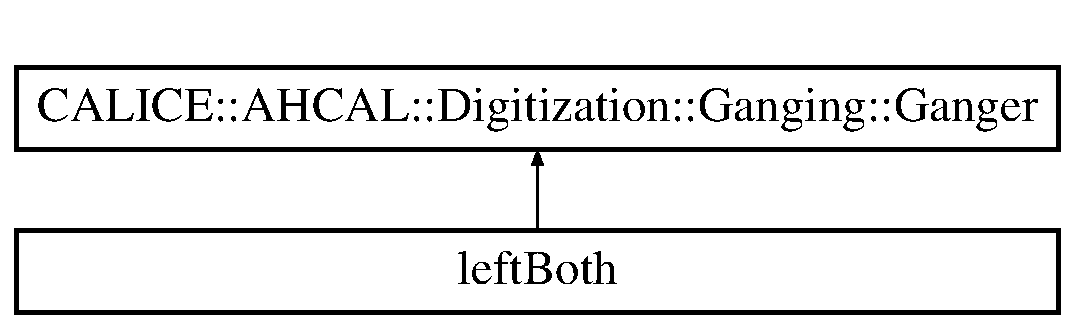
\includegraphics[height=2.000000cm]{classleftBoth}
\end{center}
\end{figure}
\subsection*{Public Member Functions}
\begin{DoxyCompactItemize}
\item 
{\bfseries left\-Both} ({\bf Contribution\-Map} $\ast$cm, float factor)\label{classleftBoth_a4f652262979a49b0037a956503f00464}

\item 
bool {\bf responsible} ({\bf Geometrical\-Indices} indices)\label{classleftBoth_aae599764d469393fa5e13d5ae54c3855}

\begin{DoxyCompactList}\small\item\em Implementations have to implement where in I/\-J they are responsible. \end{DoxyCompactList}\end{DoxyCompactItemize}


\subsection{Detailed Description}
Implementation of ganger. 

Definition at line 117 of file ahcal\-Ganging\-Processor.\-cc.



The documentation for this class was generated from the following file\-:\begin{DoxyCompactItemize}
\item 
ahcal\-Ganging\-Processor.\-cc\end{DoxyCompactItemize}

\section{digisim\-:\-:Modifier\-Parameters Class Reference}
\label{classdigisim_1_1ModifierParameters}\index{digisim\-::\-Modifier\-Parameters@{digisim\-::\-Modifier\-Parameters}}
\subsection*{Public Member Functions}
\begin{DoxyCompactItemize}
\item 
{\bfseries Modifier\-Parameters} (string name, string type, std\-::vector$<$ double $>$ \&pars)\label{classdigisim_1_1ModifierParameters_a4f6673222e35d61fc40e4a1911a5caea}

\item 
string {\bfseries get\-Type} ()\label{classdigisim_1_1ModifierParameters_a6dc5ebb8704e042999487b5dfb65c27a}

\item 
string {\bfseries get\-Name} () const \label{classdigisim_1_1ModifierParameters_ae94aec54261b77a6d7d4d1d9e8b8dfd6}

\item 
std\-::vector$<$ double $>$ {\bfseries get\-Params} () const \label{classdigisim_1_1ModifierParameters_a9178dc1b98a0c6a7589660090189f5c2}

\end{DoxyCompactItemize}
\subsection*{Private Attributes}
\begin{DoxyCompactItemize}
\item 
string {\bfseries \-\_\-type}\label{classdigisim_1_1ModifierParameters_acf6fdae58913dedcc0f6292659336142}

\item 
string {\bfseries \-\_\-name}\label{classdigisim_1_1ModifierParameters_a5868b44745451ec4ed8f86cefa5d898d}

\item 
std\-::vector$<$ double $>$ {\bfseries \-\_\-pars}\label{classdigisim_1_1ModifierParameters_afbb62698d4fbdbc85654baa4b70d1b55}

\end{DoxyCompactItemize}


\subsection{Detailed Description}


Definition at line 8 of file Modifier\-Parameters.\-hpp.



The documentation for this class was generated from the following files\-:\begin{DoxyCompactItemize}
\item 
Modifier\-Parameters.\-hpp\item 
Modifier\-Parameters.\-cpp\end{DoxyCompactItemize}

\section{Noise\-Def Class Reference}
\label{classNoiseDef}\index{Noise\-Def@{Noise\-Def}}
\subsection*{Public Member Functions}
\begin{DoxyCompactItemize}
\item 
{\bfseries Noise\-Def} (int n\-Layer, int nchannel\-X, int nchannel\-Y, std\-::vector$<$ float $>$ parameters)\label{classNoiseDef_a6b71486b7818ffdb3890915cb66e0d2e}

\item 
double {\bfseries get\-Noise} (int Layer, int channel\-X, int channel\-Y)\label{classNoiseDef_aea7dd7d26032b0037444dbe2723da59d}

\item 
double {\bfseries get\-Coherent\-Noise} (int Layer)\label{classNoiseDef_a4c2ff83a0b89a33eba1e2143b7ff9e23}

\end{DoxyCompactItemize}
\subsection*{Private Attributes}
\begin{DoxyCompactItemize}
\item 
int {\bfseries \-\_\-nlayers}\label{classNoiseDef_abd21b35506c9469adff7a2c9fe529801}

\item 
int {\bfseries \-\_\-n\-Ch\-X}\label{classNoiseDef_ac6ee3572127a83effa38dc0411895660}

\item 
int {\bfseries \-\_\-n\-Ch\-Y}\label{classNoiseDef_a9383212801004f30f5497bc16e7a6c13}

\item 
std\-::vector$<$ float $>$ {\bfseries \-\_\-par}\label{classNoiseDef_aa0f63b7ad971e2217a2a157057bcae3b}

\end{DoxyCompactItemize}


\subsection{Detailed Description}


Definition at line 6 of file Noise\-Def.\-hpp.



The documentation for this class was generated from the following file\-:\begin{DoxyCompactItemize}
\item 
Noise\-Def.\-hpp\end{DoxyCompactItemize}

\section{digisim\-:\-:Random\-Cell\-Selector Class Reference}
\label{classdigisim_1_1RandomCellSelector}\index{digisim\-::\-Random\-Cell\-Selector@{digisim\-::\-Random\-Cell\-Selector}}
\subsection*{Public Member Functions}
\begin{DoxyCompactItemize}
\item 
void {\bfseries set\-Init\-Seed} (int init\-Seed)\label{classdigisim_1_1RandomCellSelector_aa389dcac8981ac416555e2866b75d479}

\item 
void {\bf set\-Symmetry\-Order} (int symmetry\-Order)\label{classdigisim_1_1RandomCellSelector_a71fc8e3ffdc9c4a644142aeb254d3c33}

\begin{DoxyCompactList}\small\item\em Symmetry\-Order is the order of the rotational symmetry \par
 8 for an octagonal barrel calorimeter\par
 2 for an endcap calorimeter\par
 1 for a standalone prototype\par
 0 for an idealized cylindrical calorimeter. \end{DoxyCompactList}\item 
void {\bfseries setup\-Geometry} (bool use\-X\-M\-Lfile, std\-::string file\-Name=\char`\"{}\char`\"{})\label{classdigisim_1_1RandomCellSelector_aa889df9415d75c53e942f952bf9ee58b}

\item 
long long {\bfseries get\-Random\-Cell} ()\label{classdigisim_1_1RandomCellSelector_a6f0e56776338612a189c849f4981f085}

\item 
long long {\bfseries get\-Random\-Cell} (int Layer)\label{classdigisim_1_1RandomCellSelector_a42e14117b5ce129c14268f5a08a78cf1}

\item 
long long {\bfseries get\-Random\-Cell} (int Layer, int Stave, int Module)\label{classdigisim_1_1RandomCellSelector_a2cb18c5875ef99e2aee721d23e2652e1}

\item 
int {\bfseries get\-Random\-Seed} ()\label{classdigisim_1_1RandomCellSelector_aebf5a5f6c6222990afba9c56c196d4c9}

\item 
int {\bfseries get\-Total\-Number\-Of\-Cells} ()\label{classdigisim_1_1RandomCellSelector_a47ae7440cce769364e34ec878aed147e}

\item 
bool {\bfseries use\-Encoder32} ()\label{classdigisim_1_1RandomCellSelector_acae9047a8c0477530a3f66ba7f9dc242}

\item 
int {\bfseries max\-K} ()\label{classdigisim_1_1RandomCellSelector_a24a9173fd46fc5a06f3b7bba113544c1}

\item 
int {\bfseries max\-M} ()\label{classdigisim_1_1RandomCellSelector_a2fe2b6f85fdaea0b31f32589118780aa}

\item 
int {\bfseries max\-S} ()\label{classdigisim_1_1RandomCellSelector_a2364c5617141b8f2413a686bd012d7c1}

\item 
int {\bfseries max\-I} ()\label{classdigisim_1_1RandomCellSelector_ad3bb62ee1f79f2a1097d0e170607c34c}

\item 
int {\bfseries max\-J} ()\label{classdigisim_1_1RandomCellSelector_a65b2022316841b74011dbcd04cd2410f}

\end{DoxyCompactItemize}
\subsection*{Private Attributes}
\begin{DoxyCompactItemize}
\item 
gear\-::\-Gear\-Mgr $\ast$ {\bfseries \-\_\-gear\-Mgr}\label{classdigisim_1_1RandomCellSelector_ade71011e1f57476d105fc9479ab87469}

\item 
{\bf Cell\-I\-D\-Decoder} {\bfseries \-\_\-cell\-I\-D}\label{classdigisim_1_1RandomCellSelector_a1fb4b55bc5463c9d50e79459fa3e0e91}

\item 
int {\bfseries \-\_\-symmetry\-Order}\label{classdigisim_1_1RandomCellSelector_a5a3bf0a3b6f06079608c539868b28efc}

\item 
int {\bfseries \-\_\-max\-M}\label{classdigisim_1_1RandomCellSelector_a0df8bce5fad5dab347494b1494987422}

\item 
int {\bfseries \-\_\-max\-S}\label{classdigisim_1_1RandomCellSelector_ab390c4fd7f3aba78b30190e8e475fee1}

\item 
int {\bfseries \-\_\-max\-I}\label{classdigisim_1_1RandomCellSelector_aa34bf7f73f1563157ea8a2d4102ced1c}

\item 
int {\bfseries \-\_\-max\-J}\label{classdigisim_1_1RandomCellSelector_a8f193b8fd6b55a1d03fa8faeebe51e0f}

\item 
int {\bfseries \-\_\-nlayers}\label{classdigisim_1_1RandomCellSelector_a0967d00423125896764dddafd87678e0}

\item 
bool {\bfseries \-\_\-use\-Encoder32}\label{classdigisim_1_1RandomCellSelector_a82b47a95920e43853214352d1375d6b0}

\item 
int {\bfseries \-\_\-\-Layer}\label{classdigisim_1_1RandomCellSelector_aff30f83a262fa9a34856ffebaf874421}

\item 
int {\bfseries \-\_\-\-Module}\label{classdigisim_1_1RandomCellSelector_ae64969bde9ae87a8ccc594fc1e3de712}

\item 
int {\bfseries \-\_\-\-Stave}\label{classdigisim_1_1RandomCellSelector_ad50abf08f47c1485ebff9bf80ffd11d1}

\item 
T\-Random {\bfseries \-\_\-random}\label{classdigisim_1_1RandomCellSelector_aa3735334971457bee6190453076626d2}

\item 
int {\bfseries \-\_\-seed}\label{classdigisim_1_1RandomCellSelector_acf8dbe334144207374f82bc5fecb3bc1}

\item 
int {\bfseries \-\_\-num\-Tot\-Cells}\label{classdigisim_1_1RandomCellSelector_a4e709113e93171de3a57163bc96b8b9d}

\end{DoxyCompactItemize}


\subsection{Detailed Description}


Definition at line 15 of file Random\-Cell\-Selector.\-hpp.



The documentation for this class was generated from the following files\-:\begin{DoxyCompactItemize}
\item 
Random\-Cell\-Selector.\-hpp\item 
Random\-Cell\-Selector.\-cpp\end{DoxyCompactItemize}

\section{digisim\-:\-:Raw2\-Sim\-Converter Class Reference}
\label{classdigisim_1_1Raw2SimConverter}\index{digisim\-::\-Raw2\-Sim\-Converter@{digisim\-::\-Raw2\-Sim\-Converter}}


Utility class to handle the conversion of Raw\-Calorimeter\-Hits to Sim\-Calorimeter\-Hits.  




{\ttfamily \#include $<$Raw2\-Sim\-Converter.\-hpp$>$}

\subsection*{Public Member Functions}
\begin{DoxyCompactItemize}
\item 
{\bfseries Raw2\-Sim\-Converter} (double efac, double tfac)\label{classdigisim_1_1Raw2SimConverter_a3b8813468d4e04fd8376a60bf000ff7a}

\item 
void {\bfseries add\-Contribution} (const E\-V\-E\-N\-T\-::\-M\-C\-Particle $\ast$mcp, double energy, double time)\label{classdigisim_1_1Raw2SimConverter_a85735b6b24724a147e18a590b73e6d82}

\item 
I\-M\-P\-L\-::\-Sim\-Calorimeter\-Hit\-Impl $\ast$ {\bfseries convert\-To\-Sim\-Calorimeter\-Hit} ()\label{classdigisim_1_1Raw2SimConverter_acfaa9558ee8dfb5b1bad8074d2dad04f}

\item 
void {\bfseries print} ()\label{classdigisim_1_1Raw2SimConverter_a921681abcd4b3a5a47e0178f21b395c1}

\item 
void {\bfseries process} (const E\-V\-E\-N\-T\-::\-L\-C\-Collection $\ast$links)\label{classdigisim_1_1Raw2SimConverter_aeaa1d246252d1ec7ba232cccf525958d}

\item 
std\-::vector$<$ const \\*
I\-M\-P\-L\-::\-Sim\-Calorimeter\-Hit\-Impl $\ast$ $>$ \& {\bfseries get\-Sim\-Calorimeter\-Hits} ()\label{classdigisim_1_1Raw2SimConverter_ac5790f350960f5ce762e28ced791c4d3}

\item 
void {\bfseries reset} ()\label{classdigisim_1_1Raw2SimConverter_a0172859c9e945b41ece695142e633514}

\end{DoxyCompactItemize}
\subsection*{Private Types}
\begin{DoxyCompactItemize}
\item 
typedef std\-::map$<$ const \\*
E\-V\-E\-N\-T\-::\-Raw\-Calorimeter\-Hit \\*
$\ast$, I\-M\-P\-L\-::\-Sim\-Calorimeter\-Hit\-Impl $\ast$ $>$ {\bfseries Hit\-Map}\label{classdigisim_1_1Raw2SimConverter_ab7849e5504e56b9de9e197bc2c6302d1}

\end{DoxyCompactItemize}
\subsection*{Private Attributes}
\begin{DoxyCompactItemize}
\item 
double {\bfseries \-\_\-energy\-Factor}\label{classdigisim_1_1Raw2SimConverter_a929259f124928c57f1ea3e0c9959d793}

\item 
double {\bfseries \-\_\-time\-Factor}\label{classdigisim_1_1Raw2SimConverter_a3e550984ccc24b0bffdf2d970206f8c2}

\item 
std\-::vector$<$ const \\*
I\-M\-P\-L\-::\-Sim\-Calorimeter\-Hit\-Impl $\ast$ $>$ {\bfseries \-\_\-out\-Sim\-Hits}\label{classdigisim_1_1Raw2SimConverter_a39264bb7f024834813c10ff25f32928e}

\end{DoxyCompactItemize}


\subsection{Detailed Description}
Utility class to handle the conversion of Raw\-Calorimeter\-Hits to Sim\-Calorimeter\-Hits. 

\begin{DoxyAuthor}{Author}
Guilherme Lima 
\end{DoxyAuthor}


Definition at line 22 of file Raw2\-Sim\-Converter.\-hpp.



The documentation for this class was generated from the following files\-:\begin{DoxyCompactItemize}
\item 
Raw2\-Sim\-Converter.\-hpp\item 
Raw2\-Sim\-Converter.\-cpp\end{DoxyCompactItemize}

\section{digisim\-:\-:Raw\-Hit\-Converter Class Reference}
\label{classdigisim_1_1RawHitConverter}\index{digisim\-::\-Raw\-Hit\-Converter@{digisim\-::\-Raw\-Hit\-Converter}}


Utility class to handle the conversion of Raw\-Calorimeter\-Hits to Sim\-Calorimeter\-Hits.  




{\ttfamily \#include $<$Raw\-Hit\-Converter.\-hpp$>$}

\subsection*{Public Member Functions}
\begin{DoxyCompactItemize}
\item 
{\bfseries Raw\-Hit\-Converter} (double efac, double tfac)\label{classdigisim_1_1RawHitConverter_a909d99a1ec330661c8e02304f0602f1c}

\item 
void {\bfseries add\-Contribution} (const E\-V\-E\-N\-T\-::\-M\-C\-Particle $\ast$mcp, double energy, double time)\label{classdigisim_1_1RawHitConverter_a92cce974213a6c44606df731df7c4774}

\item 
I\-M\-P\-L\-::\-Calorimeter\-Hit\-Impl $\ast$ {\bfseries convert\-To\-Calorimeter\-Hit} ()\label{classdigisim_1_1RawHitConverter_a6b701f2a3f8c2d5feb97d5edbc986c53}

\item 
void {\bfseries print} ()\label{classdigisim_1_1RawHitConverter_ab9644b8058f73652976d5f46fe9b531e}

\item 
void {\bfseries process} (const E\-V\-E\-N\-T\-::\-L\-C\-Collection $\ast$links)\label{classdigisim_1_1RawHitConverter_abfb84ba443d5b31266cb1ea69233bc0e}

\item 
void {\bfseries process} (const E\-V\-E\-N\-T\-::\-L\-C\-Collection $\ast$links, E\-V\-E\-N\-T\-::\-L\-C\-Collection $\ast$relcol)\label{classdigisim_1_1RawHitConverter_a0d58fb0019e6bc609a8f4c898f77ffe8}

\item 
std\-::vector$<$ const \\*
I\-M\-P\-L\-::\-Calorimeter\-Hit\-Impl $\ast$ $>$ \& {\bfseries get\-Calorimeter\-Hits} ()\label{classdigisim_1_1RawHitConverter_a5b146d8a5f1a24ed89f7a015668728c4}

\item 
void {\bfseries reset} ()\label{classdigisim_1_1RawHitConverter_a17b8e571f1047c902983dfc2c720f717}

\end{DoxyCompactItemize}
\subsection*{Private Types}
\begin{DoxyCompactItemize}
\item 
typedef std\-::map$<$ const \\*
E\-V\-E\-N\-T\-::\-Raw\-Calorimeter\-Hit \\*
$\ast$, I\-M\-P\-L\-::\-Calorimeter\-Hit\-Impl $\ast$ $>$ {\bfseries Hit\-Map}\label{classdigisim_1_1RawHitConverter_a758d21158f1bcfeab05338272405378b}

\end{DoxyCompactItemize}
\subsection*{Private Attributes}
\begin{DoxyCompactItemize}
\item 
double {\bfseries \-\_\-energy\-Factor}\label{classdigisim_1_1RawHitConverter_a9a910a84c29119a74a2ad3fe3e0cb137}

\item 
double {\bfseries \-\_\-time\-Factor}\label{classdigisim_1_1RawHitConverter_aee3caecdb0f171d2168bd28d0ca4de20}

\item 
std\-::vector$<$ const \\*
I\-M\-P\-L\-::\-Calorimeter\-Hit\-Impl $\ast$ $>$ {\bfseries \-\_\-out\-Cal\-Hits}\label{classdigisim_1_1RawHitConverter_aa8d3b0a3603e8d6036c2bca684373513}

\end{DoxyCompactItemize}


\subsection{Detailed Description}
Utility class to handle the conversion of Raw\-Calorimeter\-Hits to Sim\-Calorimeter\-Hits. 

\begin{DoxyAuthor}{Author}
Guilherme Lima 
\end{DoxyAuthor}


Definition at line 23 of file Raw\-Hit\-Converter.\-hpp.



The documentation for this class was generated from the following files\-:\begin{DoxyCompactItemize}
\item 
Raw\-Hit\-Converter.\-hpp\item 
Raw\-Hit\-Converter.\-cpp\end{DoxyCompactItemize}

\section{right\-Both Class Reference}
\label{classrightBoth}\index{right\-Both@{right\-Both}}


Implementation of ganger.  


Inheritance diagram for right\-Both\-:\begin{figure}[H]
\begin{center}
\leavevmode
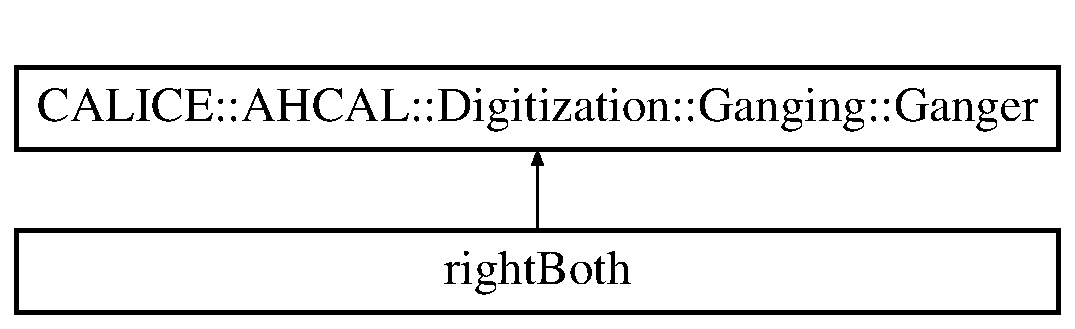
\includegraphics[height=2.000000cm]{classrightBoth}
\end{center}
\end{figure}
\subsection*{Public Member Functions}
\begin{DoxyCompactItemize}
\item 
{\bfseries right\-Both} ({\bf Contribution\-Map} $\ast$cm, float factor)\label{classrightBoth_a3fedb57d99908019a6e9beda9274686c}

\item 
bool {\bf responsible} ({\bf Geometrical\-Indices} indices)\label{classrightBoth_a5b87c7eaa01c916053e5e66b250c43b8}

\begin{DoxyCompactList}\small\item\em Implementations have to implement where in I/\-J they are responsible. \end{DoxyCompactList}\end{DoxyCompactItemize}


\subsection{Detailed Description}
Implementation of ganger. 

Definition at line 151 of file ahcal\-Ganging\-Processor.\-cc.



The documentation for this class was generated from the following file\-:\begin{DoxyCompactItemize}
\item 
ahcal\-Ganging\-Processor.\-cc\end{DoxyCompactItemize}

\section{ring\-Fine Class Reference}
\label{classringFine}\index{ring\-Fine@{ring\-Fine}}


Implementation of ganger.  


Inheritance diagram for ring\-Fine\-:\begin{figure}[H]
\begin{center}
\leavevmode
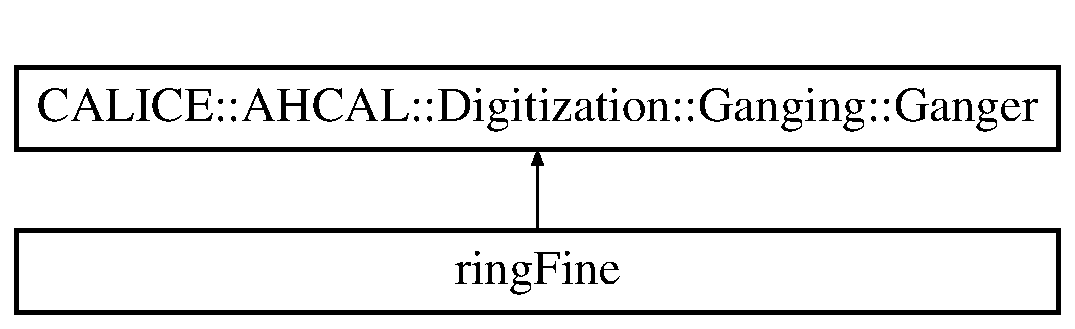
\includegraphics[height=2.000000cm]{classringFine}
\end{center}
\end{figure}
\subsection*{Public Member Functions}
\begin{DoxyCompactItemize}
\item 
{\bfseries ring\-Fine} ({\bf Contribution\-Map} $\ast$cm, float factor)\label{classringFine_ab81a07c350ce3b1a4b0ace414f616f8a}

\item 
bool {\bf responsible} ({\bf Geometrical\-Indices} indices)\label{classringFine_a17303f8b6005ba65a381161aa632ff29}

\begin{DoxyCompactList}\small\item\em Implementations have to implement where in I/\-J they are responsible. \end{DoxyCompactList}\end{DoxyCompactItemize}


\subsection{Detailed Description}
Implementation of ganger. 

Definition at line 61 of file ahcal\-Ganging\-Processor.\-cc.



The documentation for this class was generated from the following file\-:\begin{DoxyCompactItemize}
\item 
ahcal\-Ganging\-Processor.\-cc\end{DoxyCompactItemize}

\section{Sc\-E\-C\-A\-L\-Digitizer Class Reference}
\label{classScECALDigitizer}\index{Sc\-E\-C\-A\-L\-Digitizer@{Sc\-E\-C\-A\-L\-Digitizer}}


Example processor for marlin.  




{\ttfamily \#include $<$Sc\-E\-C\-A\-L\-Digitizer.\-hh$>$}

Inheritance diagram for Sc\-E\-C\-A\-L\-Digitizer\-:\begin{figure}[H]
\begin{center}
\leavevmode
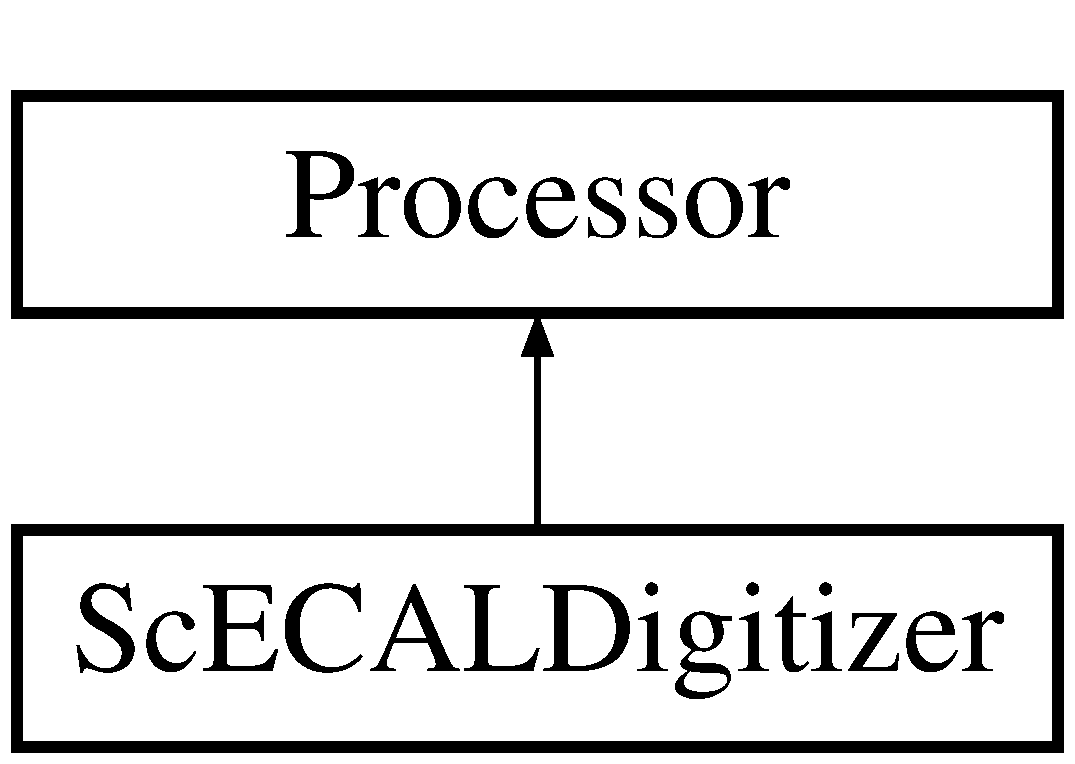
\includegraphics[height=2.000000cm]{classScECALDigitizer}
\end{center}
\end{figure}
\subsection*{Public Member Functions}
\begin{DoxyCompactItemize}
\item 
virtual Processor $\ast$ {\bfseries new\-Processor} ()\label{classScECALDigitizer_afc1b1dc86364bd86e8434521f0d14a8e}

\item 
virtual void {\bf init} ()
\begin{DoxyCompactList}\small\item\em Called at the begin of the job before anything is read. \end{DoxyCompactList}\item 
virtual void {\bf process\-Run\-Header} (L\-C\-Run\-Header $\ast$run)\label{classScECALDigitizer_adf8adb4733c400a5ceb5f345d2b00058}

\begin{DoxyCompactList}\small\item\em Called for every run. \end{DoxyCompactList}\item 
virtual void {\bf process\-Event} (L\-C\-Event $\ast$evt)\label{classScECALDigitizer_a68882c5b15e60cef5cb8524e5c14c1fb}

\begin{DoxyCompactList}\small\item\em Called for every event -\/ the working horse. \end{DoxyCompactList}\item 
virtual void {\bfseries check} (L\-C\-Event $\ast$evt)\label{classScECALDigitizer_afe24458ee3d08501d2ceb7e60a262f21}

\item 
virtual void {\bf end} ()\label{classScECALDigitizer_a8194e795626a3b1b85c792d9333485a3}

\begin{DoxyCompactList}\small\item\em Called after data processing for clean up. \end{DoxyCompactList}\end{DoxyCompactItemize}
\subsection*{Protected Attributes}
\begin{DoxyCompactItemize}
\item 
std\-::string {\bf \-\_\-col\-Name}\label{classScECALDigitizer_a3caef161c2472e7a6fea690ebd012f09}

\begin{DoxyCompactList}\small\item\em Input collection name. \end{DoxyCompactList}\item 
int {\bfseries \-\_\-n\-Run}\label{classScECALDigitizer_a8ddac6c05e16590e133456f5943d0cb7}

\item 
int {\bfseries \-\_\-n\-Evt}\label{classScECALDigitizer_a9a3a3d29ed875c5c574758478e22c073}

\item 
std\-::vector$<$ std\-::string $>$ {\bfseries \-\_\-ecal\-Collections}\label{classScECALDigitizer_aa50779725972af8eca079f0f387d7ada}

\item 
std\-::vector$<$ std\-::string $>$ {\bfseries \-\_\-output\-Ecal\-Collections}\label{classScECALDigitizer_a6d5c0ffec0c55841a3babfcface65562}

\item 
std\-::string {\bfseries \-\_\-root\-File\-Name}\label{classScECALDigitizer_ac8773de7d9ebb49cf5325649c61efcbd}

\item 
T\-File $\ast$ {\bfseries f\-File}\label{classScECALDigitizer_aa733d8db74513188e98a19f702edbc59}

\item 
T\-H1\-D $\ast$ {\bfseries f\-Hist}\label{classScECALDigitizer_a85dc4831515dc7e435c29e952ece8c3a}

\item 
T\-Ntuple $\ast$ {\bfseries f\-N\-Events}\label{classScECALDigitizer_a3689782b7b5a2c3fa02171dd14a54042}

\item 
T\-Ntuple $\ast$ {\bfseries f\-N\-Hits}\label{classScECALDigitizer_a1bd33e27ad6c92e30d3f4c5affa159a4}

\item 
float {\bfseries \-\_\-threshold\-Ecal}\label{classScECALDigitizer_abd2bd9a8ff79b668e2c4f058f762e0aa}

\item 
float {\bfseries \-\_\-calibr\-Coeff\-Ecal}\label{classScECALDigitizer_a1b592b3432ee22760a31f2701edec4ed}

\end{DoxyCompactItemize}


\subsection{Detailed Description}
Example processor for marlin. 

If compiled with M\-A\-R\-L\-I\-N\-\_\-\-U\-S\-E\-\_\-\-A\-I\-D\-A it creates a histogram (cloud) of the M\-C\-Particle energies.

\subparagraph*{Input -\/ Prerequisites}

Needs the collection of M\-C\-Particles.

\subparagraph*{Output}

A histogram.


\begin{DoxyParams}{Parameters}
{\em Collection\-Name} & Name of the M\-C\-Particle collection\\
\hline
\end{DoxyParams}
\begin{DoxyAuthor}{Author}
F. Gaede, D\-E\-S\-Y 
\end{DoxyAuthor}
\begin{DoxyVersion}{Version}

\end{DoxyVersion}
\begin{DoxyParagraph}{Id\-:}
My\-Processor.\-h,v 1.\-4 2005/10/11 12\-:57\-:39 gaede Exp 
\end{DoxyParagraph}


Definition at line 33 of file Sc\-E\-C\-A\-L\-Digitizer.\-hh.



\subsection{Member Function Documentation}
\index{Sc\-E\-C\-A\-L\-Digitizer@{Sc\-E\-C\-A\-L\-Digitizer}!init@{init}}
\index{init@{init}!ScECALDigitizer@{Sc\-E\-C\-A\-L\-Digitizer}}
\subsubsection[{init}]{\setlength{\rightskip}{0pt plus 5cm}virtual void Sc\-E\-C\-A\-L\-Digitizer\-::init (
\begin{DoxyParamCaption}
{}
\end{DoxyParamCaption}
)\hspace{0.3cm}{\ttfamily [virtual]}}\label{classScECALDigitizer_a58e026eb43e35501805e3f3d0e7f3786}


Called at the begin of the job before anything is read. 

Use to initialize the processor, e.\-g. book histograms. 

The documentation for this class was generated from the following file\-:\begin{DoxyCompactItemize}
\item 
Sc\-E\-C\-A\-L\-Digitizer.\-hh\end{DoxyCompactItemize}

\section{digisim\-:\-:Sim\-Calorimeter\-Hits\-Processor Class Reference}
\label{classdigisim_1_1SimCalorimeterHitsProcessor}\index{digisim\-::\-Sim\-Calorimeter\-Hits\-Processor@{digisim\-::\-Sim\-Calorimeter\-Hits\-Processor}}
Inheritance diagram for digisim\-:\-:Sim\-Calorimeter\-Hits\-Processor\-:\begin{figure}[H]
\begin{center}
\leavevmode
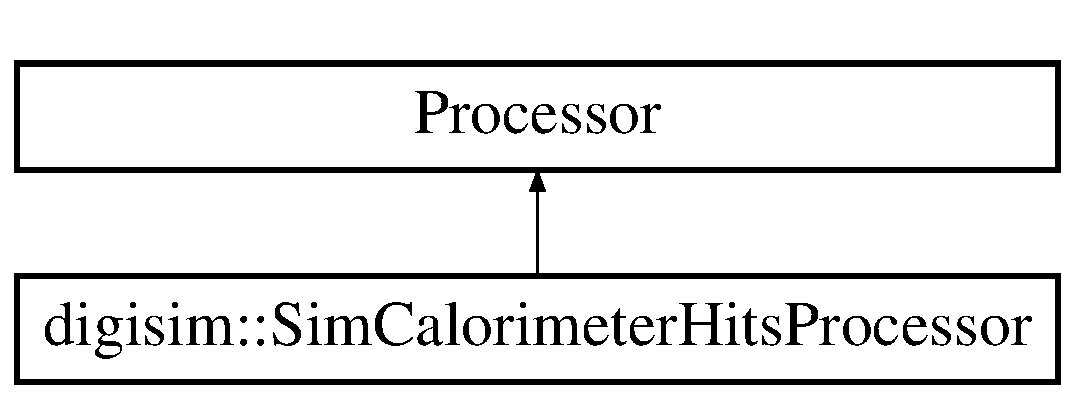
\includegraphics[height=2.000000cm]{classdigisim_1_1SimCalorimeterHitsProcessor}
\end{center}
\end{figure}
\subsection*{Public Member Functions}
\begin{DoxyCompactItemize}
\item 
virtual Processor $\ast$ {\bfseries new\-Processor} ()\label{classdigisim_1_1SimCalorimeterHitsProcessor_a0167d5d99f039550ff02ae2c6053f1e4}

\item 
virtual void {\bf init} ()
\begin{DoxyCompactList}\small\item\em Called at the begin of the job before anything is read. \end{DoxyCompactList}\item 
virtual void {\bf process\-Event} (L\-C\-Event $\ast$evt)
\begin{DoxyCompactList}\small\item\em Called for every run. \end{DoxyCompactList}\item 
virtual void {\bf end} ()\label{classdigisim_1_1SimCalorimeterHitsProcessor_a415577954cca081b450fd0a608560529}

\begin{DoxyCompactList}\small\item\em Called after data processing for clean up. \end{DoxyCompactList}\end{DoxyCompactItemize}
\subsection*{Protected Attributes}
\begin{DoxyCompactItemize}
\item 
L\-C\-Event $\ast$ {\bfseries \-\_\-evt}\label{classdigisim_1_1SimCalorimeterHitsProcessor_abd5a88f643a6ff8b4a2f42bca5909fe8}

\item 
std\-::vector$<$ std\-::string $>$ {\bfseries \-\_\-raw\-Names}\label{classdigisim_1_1SimCalorimeterHitsProcessor_ae70e4f720684c6836f7341b639b32f17}

\item 
std\-::vector$<$ std\-::string $>$ {\bfseries \-\_\-link\-Names}\label{classdigisim_1_1SimCalorimeterHitsProcessor_a969829cd4ae399f8012ee38c790bd6fa}

\item 
std\-::vector$<$ std\-::string $>$ {\bfseries \-\_\-output\-Names}\label{classdigisim_1_1SimCalorimeterHitsProcessor_ac30ad5b4d57c5c983a6c840ca3a988ee}

\item 
double {\bfseries \-\_\-ene\-Factor}\label{classdigisim_1_1SimCalorimeterHitsProcessor_a7be096df555305c582986a4048c2db66}

\item 
double {\bfseries \-\_\-time\-Factor}\label{classdigisim_1_1SimCalorimeterHitsProcessor_a89c7b96076328bd999480165b9b8993c}

\item 
int {\bfseries \-\_\-n\-Run}\label{classdigisim_1_1SimCalorimeterHitsProcessor_abf27722a302a66a718722009882e37af}

\item 
int {\bfseries \-\_\-n\-Evt}\label{classdigisim_1_1SimCalorimeterHitsProcessor_a78e7e5a57ea47b1fe85d8335d73e360b}

\item 
std\-::map$<$ const \\*
E\-V\-E\-N\-T\-::\-Raw\-Calorimeter\-Hit \\*
$\ast$, std\-::vector$<$ const \\*
E\-V\-E\-N\-T\-::\-L\-C\-Relation $\ast$ $>$ $\ast$ $>$ $\ast$ {\bfseries \-\_\-links\-Map}\label{classdigisim_1_1SimCalorimeterHitsProcessor_a4391c1811ba2ccea77a3c1a0df009151}

\item 
{\bf Raw2\-Sim\-Converter} $\ast$ {\bfseries \-\_\-converter}\label{classdigisim_1_1SimCalorimeterHitsProcessor_a6943e3c363a9272114a8b9f523c88486}

\end{DoxyCompactItemize}
\subsection*{Private Member Functions}
\begin{DoxyCompactItemize}
\item 
E\-V\-E\-N\-T\-::\-L\-C\-Collection $\ast$ {\bfseries create\-Output\-Collection} (const std\-::vector$<$ const I\-M\-P\-L\-::\-Sim\-Calorimeter\-Hit\-Impl $\ast$ $>$ \&newhits)\label{classdigisim_1_1SimCalorimeterHitsProcessor_ab346f980ae3d444d89bd61ac9b558bfd}

\item 
void {\bfseries clear\-Links\-Map} ()\label{classdigisim_1_1SimCalorimeterHitsProcessor_a651df6cc5857e5defa3ded96b7ee1d7f}

\end{DoxyCompactItemize}


\subsection{Detailed Description}


Definition at line 25 of file Sim\-Calorimeter\-Hits\-Processor.\-hpp.



\subsection{Member Function Documentation}
\index{digisim\-::\-Sim\-Calorimeter\-Hits\-Processor@{digisim\-::\-Sim\-Calorimeter\-Hits\-Processor}!init@{init}}
\index{init@{init}!digisim::SimCalorimeterHitsProcessor@{digisim\-::\-Sim\-Calorimeter\-Hits\-Processor}}
\subsubsection[{init}]{\setlength{\rightskip}{0pt plus 5cm}void digisim\-::\-Sim\-Calorimeter\-Hits\-Processor\-::init (
\begin{DoxyParamCaption}
{}
\end{DoxyParamCaption}
)\hspace{0.3cm}{\ttfamily [virtual]}}\label{classdigisim_1_1SimCalorimeterHitsProcessor_a0db07062a94c58566e7d6e9ec76269ad}


Called at the begin of the job before anything is read. 

Use to initialize the processor, e.\-g. book histograms. 

Definition at line 164 of file Sim\-Calorimeter\-Hits\-Processor.\-cpp.

\index{digisim\-::\-Sim\-Calorimeter\-Hits\-Processor@{digisim\-::\-Sim\-Calorimeter\-Hits\-Processor}!process\-Event@{process\-Event}}
\index{process\-Event@{process\-Event}!digisim::SimCalorimeterHitsProcessor@{digisim\-::\-Sim\-Calorimeter\-Hits\-Processor}}
\subsubsection[{process\-Event}]{\setlength{\rightskip}{0pt plus 5cm}void digisim\-::\-Sim\-Calorimeter\-Hits\-Processor\-::process\-Event (
\begin{DoxyParamCaption}
\item[{L\-C\-Event $\ast$}]{evt}
\end{DoxyParamCaption}
)\hspace{0.3cm}{\ttfamily [virtual]}}\label{classdigisim_1_1SimCalorimeterHitsProcessor_aa4a52f270887036315f7fde324a45fd8}


Called for every run. 

Called for every event 

Definition at line 82 of file Sim\-Calorimeter\-Hits\-Processor.\-cpp.



The documentation for this class was generated from the following files\-:\begin{DoxyCompactItemize}
\item 
Sim\-Calorimeter\-Hits\-Processor.\-hpp\item 
Sim\-Calorimeter\-Hits\-Processor.\-cpp\end{DoxyCompactItemize}

\section{digisim\-:\-:Si\-P\-M\-Saturation Class Reference}
\label{classdigisim_1_1SiPMSaturation}\index{digisim\-::\-Si\-P\-M\-Saturation@{digisim\-::\-Si\-P\-M\-Saturation}}
Inheritance diagram for digisim\-:\-:Si\-P\-M\-Saturation\-:\begin{figure}[H]
\begin{center}
\leavevmode
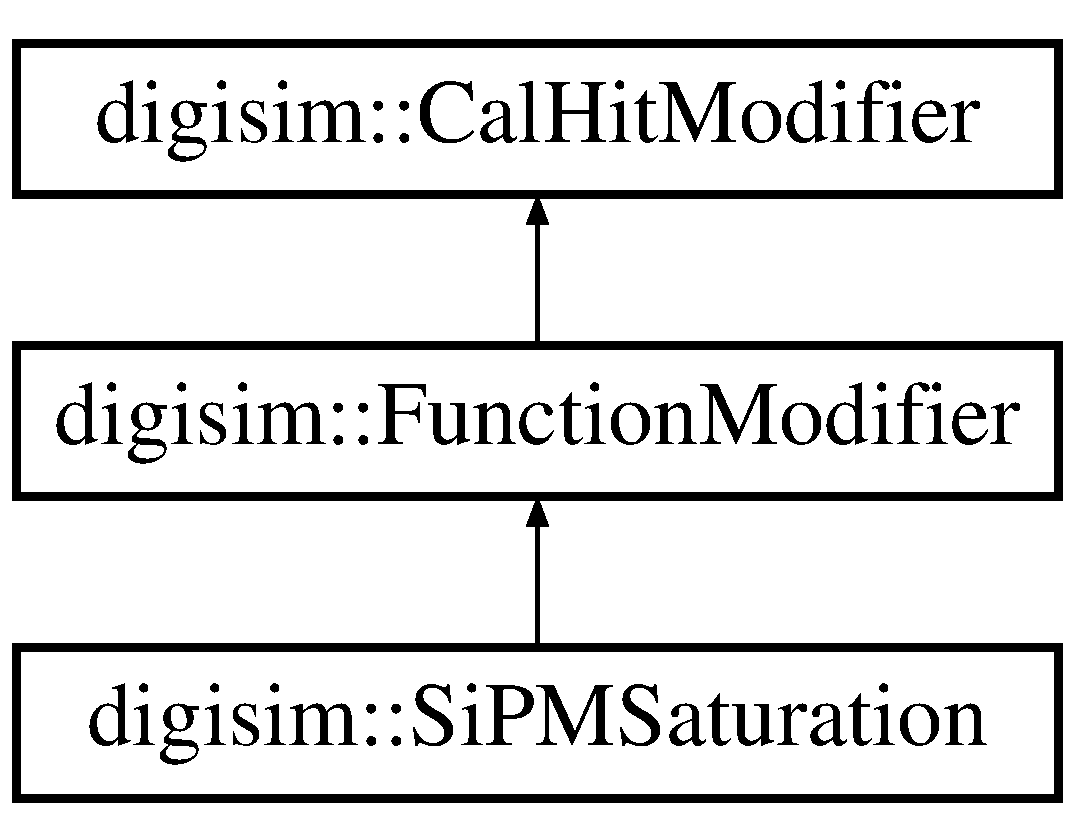
\includegraphics[height=3.000000cm]{classdigisim_1_1SiPMSaturation}
\end{center}
\end{figure}
\subsection*{Public Member Functions}
\begin{DoxyCompactItemize}
\item 
{\bf Si\-P\-M\-Saturation} ()\label{classdigisim_1_1SiPMSaturation_a77b92130d1b442ed69650a68415b3ec1}

\begin{DoxyCompactList}\small\item\em default constructor is only called for global instance \end{DoxyCompactList}\item 
{\bf Si\-P\-M\-Saturation} $\ast$ {\bf new\-Instance} (const std\-::string \&mod\-Name)\label{classdigisim_1_1SiPMSaturation_a04904d305e9bf5b811c1b9dff88341d7}

\begin{DoxyCompactList}\small\item\em Returns a reference to a new instance. \end{DoxyCompactList}\item 
double {\bf transform\-Energy} (const {\bf Temp\-Cal\-Hit} \&hit) const \label{classdigisim_1_1SiPMSaturation_ae16cb8ee6fe533c3dc76d6cecfc9a821}

\begin{DoxyCompactList}\small\item\em Smeared linear transformations on energy. \end{DoxyCompactList}\end{DoxyCompactItemize}
\subsection*{Private Member Functions}
\begin{DoxyCompactItemize}
\item 
{\bfseries Si\-P\-M\-Saturation} (const std\-::string \&mod\-Name)\label{classdigisim_1_1SiPMSaturation_a35080e707c417dbb1cce6a4681a35ee2}

\item 
{\bfseries Si\-P\-M\-Saturation} (const {\bf Si\-P\-M\-Saturation} \&rhs)\label{classdigisim_1_1SiPMSaturation_a05ba0d472061dbb62bffae1eefbd0450}

\end{DoxyCompactItemize}
\subsection*{Additional Inherited Members}


\subsection{Detailed Description}


Definition at line 12 of file Si\-P\-M\-Saturation.\-hpp.



The documentation for this class was generated from the following files\-:\begin{DoxyCompactItemize}
\item 
Si\-P\-M\-Saturation.\-hpp\item 
Si\-P\-M\-Saturation.\-cpp\end{DoxyCompactItemize}

\section{digisim\-:\-:Smeared\-Gain Class Reference}
\label{classdigisim_1_1SmearedGain}\index{digisim\-::\-Smeared\-Gain@{digisim\-::\-Smeared\-Gain}}
Inheritance diagram for digisim\-:\-:Smeared\-Gain\-:\begin{figure}[H]
\begin{center}
\leavevmode
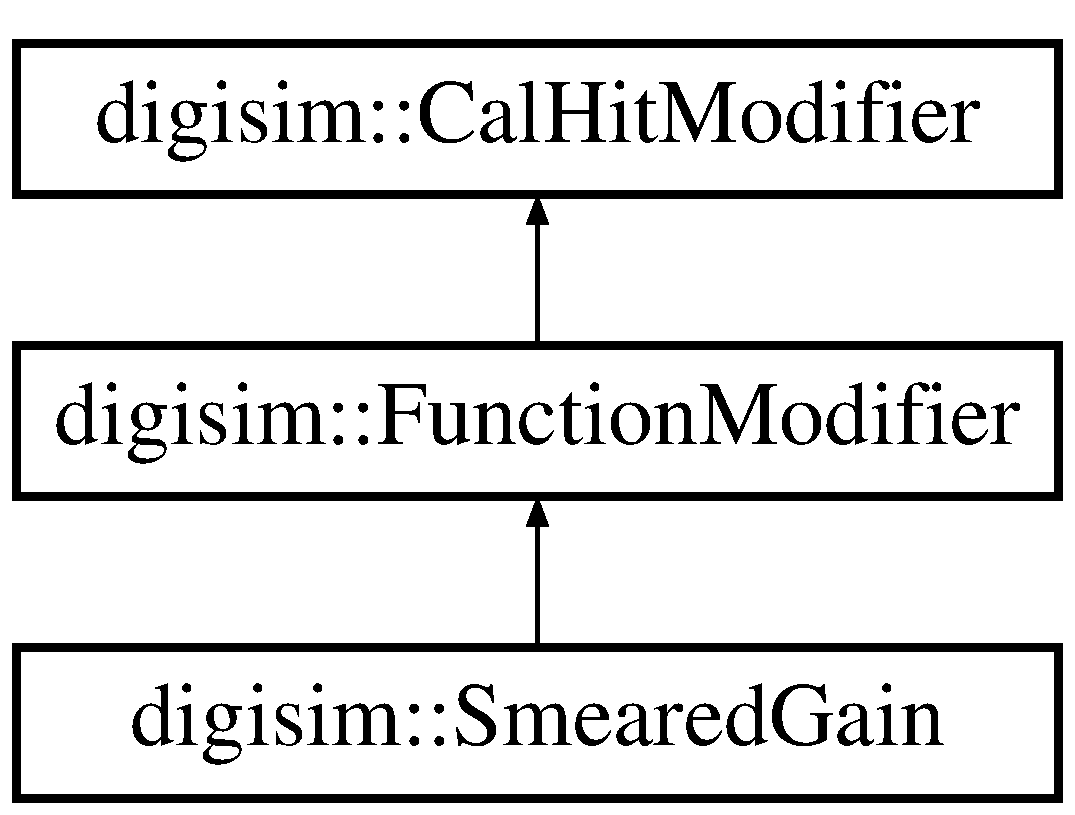
\includegraphics[height=3.000000cm]{classdigisim_1_1SmearedGain}
\end{center}
\end{figure}
\subsection*{Public Member Functions}
\begin{DoxyCompactItemize}
\item 
{\bf Smeared\-Gain} $\ast$ {\bf new\-Instance} (const std\-::string \&mod\-Name)\label{classdigisim_1_1SmearedGain_ab9cc71705f9d57c9bbc2f5626d99fd6c}

\begin{DoxyCompactList}\small\item\em Returns a reference to a new instance. \end{DoxyCompactList}\item 
{\bf Smeared\-Gain} ()\label{classdigisim_1_1SmearedGain_a0101aee74eb896cf065bcc7a9cfff390}

\begin{DoxyCompactList}\small\item\em default constructor is only called for global instance \end{DoxyCompactList}\item 
double {\bf transform\-Energy} (const {\bf Temp\-Cal\-Hit} \&hit) const 
\begin{DoxyCompactList}\small\item\em Smeared linear transformations on time. \end{DoxyCompactList}\end{DoxyCompactItemize}
\subsection*{Private Member Functions}
\begin{DoxyCompactItemize}
\item 
{\bfseries Smeared\-Gain} (const std\-::string \&mod\-Name)\label{classdigisim_1_1SmearedGain_a41782999a91d81204766e0e9ab3f6bb8}

\item 
{\bfseries Smeared\-Gain} (const {\bf Smeared\-Gain} \&rhs)\label{classdigisim_1_1SmearedGain_a5708783eec75b63800d9a09d2899ee14}

\end{DoxyCompactItemize}
\subsection*{Additional Inherited Members}


\subsection{Detailed Description}


Definition at line 11 of file Smeared\-Gain.\-hpp.



\subsection{Member Function Documentation}
\index{digisim\-::\-Smeared\-Gain@{digisim\-::\-Smeared\-Gain}!transform\-Energy@{transform\-Energy}}
\index{transform\-Energy@{transform\-Energy}!digisim::SmearedGain@{digisim\-::\-Smeared\-Gain}}
\subsubsection[{transform\-Energy}]{\setlength{\rightskip}{0pt plus 5cm}double digisim\-::\-Smeared\-Gain\-::transform\-Energy (
\begin{DoxyParamCaption}
\item[{const {\bf Temp\-Cal\-Hit} \&}]{hit}
\end{DoxyParamCaption}
) const\hspace{0.3cm}{\ttfamily [virtual]}}\label{classdigisim_1_1SmearedGain_a661e2ca73a32303f0bd59ce62b48559a}


Smeared linear transformations on time. 

Smeared linear transformations on energy. 

Implements {\bf digisim\-::\-Function\-Modifier} \doxyref{}{p.}{classdigisim_1_1FunctionModifier}.



Definition at line 26 of file Smeared\-Gain.\-cpp.



The documentation for this class was generated from the following files\-:\begin{DoxyCompactItemize}
\item 
Smeared\-Gain.\-hpp\item 
Smeared\-Gain.\-cpp\end{DoxyCompactItemize}

\section{digisim\-:\-:Smeared\-Timing Class Reference}
\label{classdigisim_1_1SmearedTiming}\index{digisim\-::\-Smeared\-Timing@{digisim\-::\-Smeared\-Timing}}
Inheritance diagram for digisim\-:\-:Smeared\-Timing\-:\begin{figure}[H]
\begin{center}
\leavevmode
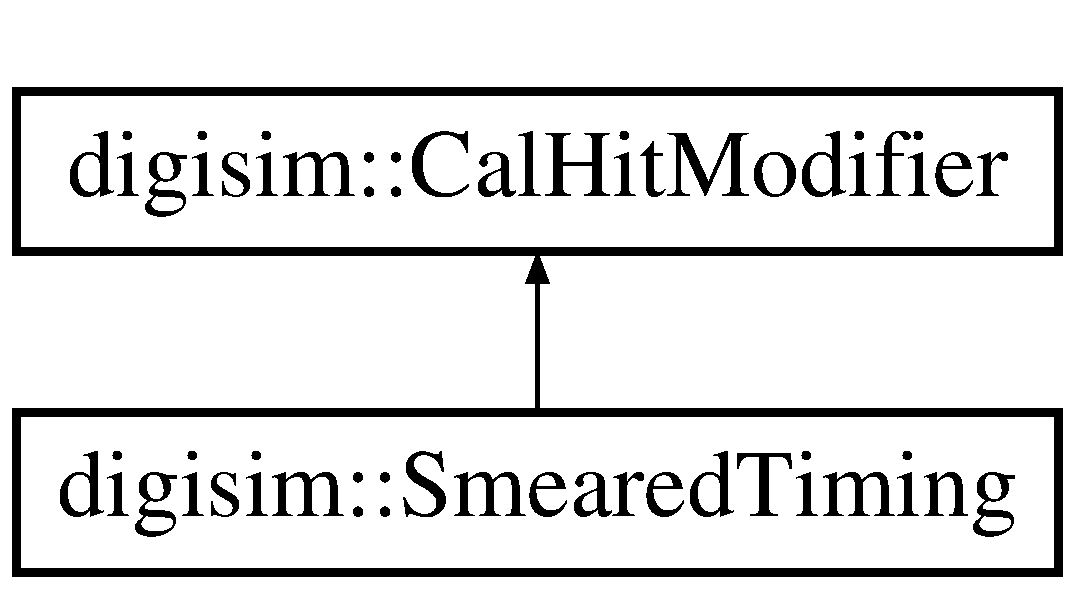
\includegraphics[height=2.000000cm]{classdigisim_1_1SmearedTiming}
\end{center}
\end{figure}
\subsection*{Public Member Functions}
\begin{DoxyCompactItemize}
\item 
{\bf Smeared\-Timing} $\ast$ {\bf new\-Instance} (const std\-::string \&mod\-Name)\label{classdigisim_1_1SmearedTiming_a100c03fd016ab2747ef91ca484e86ac5}

\begin{DoxyCompactList}\small\item\em Returns a reference to a new instance. \end{DoxyCompactList}\item 
{\bf Smeared\-Timing} ()\label{classdigisim_1_1SmearedTiming_ad1de97af7e1f49556c31f9761a7251f9}

\begin{DoxyCompactList}\small\item\em default constructor is only called for global instance \end{DoxyCompactList}\item 
void {\bf init} (std\-::vector$<$ float $>$ \&floats)\label{classdigisim_1_1SmearedTiming_a7dcecdda4d162208887cc59df10235a0}

\begin{DoxyCompactList}\small\item\em initialize parameters \end{DoxyCompactList}\item 
void {\bfseries process\-Hits} (std\-::map$<$ long long, {\bf Temp\-Cal\-Hit} $>$ \&hitmap)\label{classdigisim_1_1SmearedTiming_ac39257e23e67cb167164cdf27a53d9b0}

\item 
double {\bf transform\-Time} (const {\bf Temp\-Cal\-Hit} \&hit)\label{classdigisim_1_1SmearedTiming_ac061272e8d099d7448b636b691af7db2}

\begin{DoxyCompactList}\small\item\em Smeared linear transformations on time. \end{DoxyCompactList}\item 
void {\bf print} () const \label{classdigisim_1_1SmearedTiming_aa801b4cb37d9cd384a0f3698e2f5aa9d}

\begin{DoxyCompactList}\small\item\em debugging printout \end{DoxyCompactList}\end{DoxyCompactItemize}
\subsection*{Private Member Functions}
\begin{DoxyCompactItemize}
\item 
{\bfseries Smeared\-Timing} (const std\-::string \&mod\-Name)\label{classdigisim_1_1SmearedTiming_a145f06b6464795163fe3e155a0e61e1c}

\item 
{\bfseries Smeared\-Timing} (const {\bf Smeared\-Timing} \&rhs)\label{classdigisim_1_1SmearedTiming_a642b9104cc973966ef4a7a16761cdb9d}

\end{DoxyCompactItemize}
\subsection*{Private Attributes}
\begin{DoxyCompactItemize}
\item 
std\-::vector$<$ float $>$ {\bf \-\_\-par}\label{classdigisim_1_1SmearedTiming_ae561a940d1502fd5194184320ca9d8a4}

\begin{DoxyCompactList}\small\item\em Parameters\-: gain and threshold. \end{DoxyCompactList}\end{DoxyCompactItemize}
\subsection*{Additional Inherited Members}


\subsection{Detailed Description}


Definition at line 11 of file Smeared\-Timing.\-hpp.



The documentation for this class was generated from the following files\-:\begin{DoxyCompactItemize}
\item 
Smeared\-Timing.\-hpp\item 
Smeared\-Timing.\-cpp\end{DoxyCompactItemize}

\section{C\-A\-L\-I\-C\-E\-:\-:T\-B\-Ecal\-Digitisation Class Reference}
\label{classCALICE_1_1TBEcalDigitisation}\index{C\-A\-L\-I\-C\-E\-::\-T\-B\-Ecal\-Digitisation@{C\-A\-L\-I\-C\-E\-::\-T\-B\-Ecal\-Digitisation}}


File\-: T\-B\-Ecal\-Digitisation.\-hpp.  




{\ttfamily \#include $<$T\-B\-Ecal\-Digitisation.\-hh$>$}

Inheritance diagram for C\-A\-L\-I\-C\-E\-:\-:T\-B\-Ecal\-Digitisation\-:\begin{figure}[H]
\begin{center}
\leavevmode
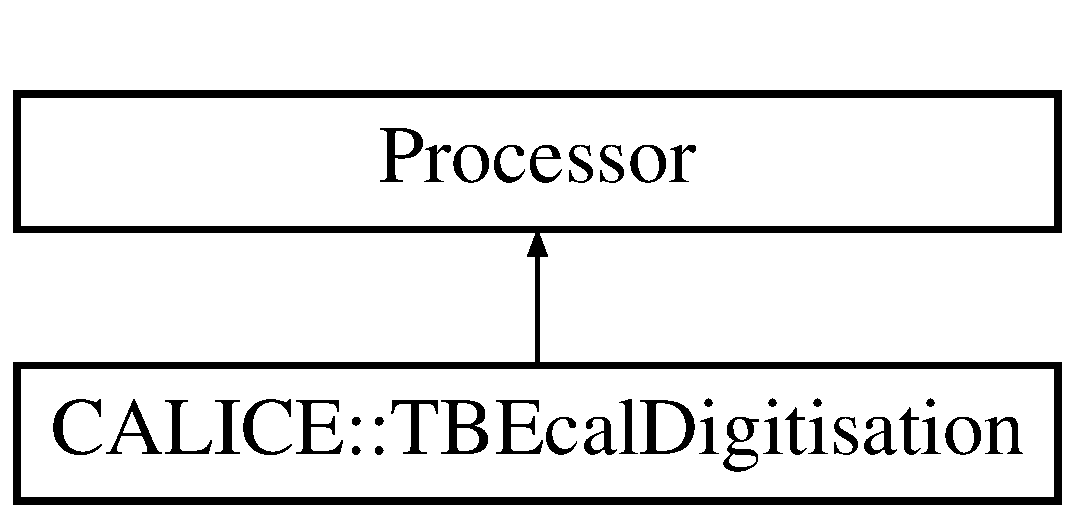
\includegraphics[height=2.000000cm]{classCALICE_1_1TBEcalDigitisation}
\end{center}
\end{figure}
\subsection*{Public Member Functions}
\begin{DoxyCompactItemize}
\item 
virtual Processor $\ast$ {\bfseries new\-Processor} ()\label{classCALICE_1_1TBEcalDigitisation_ac21322be565c00420729ed4eda6edf06}

\item 
virtual void {\bf init} ()
\begin{DoxyCompactList}\small\item\em Called at the begin of the job before anything is read. \end{DoxyCompactList}\item 
virtual void {\bf process\-Run\-Header} (L\-C\-Run\-Header $\ast$run)\label{classCALICE_1_1TBEcalDigitisation_ab68d8f2ddd5cb8a2167fd2cd7ef820ec}

\begin{DoxyCompactList}\small\item\em Called for every run. \end{DoxyCompactList}\item 
virtual void {\bf process\-Event} (L\-C\-Event $\ast$evt)\label{classCALICE_1_1TBEcalDigitisation_af7e2e52733cec587256fb883a86416ab}

\begin{DoxyCompactList}\small\item\em Called for every event -\/ the working horse. \end{DoxyCompactList}\item 
virtual void {\bf end} ()\label{classCALICE_1_1TBEcalDigitisation_a96a298b34d073351fea166cee60bd366}

\begin{DoxyCompactList}\small\item\em Called after data processing for clean up. \end{DoxyCompactList}\item 
void {\bfseries Decalibrate\-Hits} (double \&hitenergy, int cell\-I\-D0, int \&cell\-I\-D1)\label{classCALICE_1_1TBEcalDigitisation_ad0455f25a8e64078fb21e6bcd4062b2d}

\item 
void {\bfseries Fill\-Random\-Noise} ()\label{classCALICE_1_1TBEcalDigitisation_a76557d9096949f5ccd6ee71c0f23590a}

\item 
void {\bfseries set\-Noise\-Cell\-I\-Ds} (int \&cell\-I\-D0, int \&cell\-I\-D1, int lay, int waf, int ch)\label{classCALICE_1_1TBEcalDigitisation_ab2712d0b84c441c1205c594f9796ded5}

\end{DoxyCompactItemize}
\subsection*{Static Public Member Functions}
\begin{DoxyCompactItemize}
\item 
static \\*
C\-A\-L\-I\-C\-E\-::\-Noise\-Parameter\-Arrayof\-Array\-\_\-t \& {\bfseries get\-Cell\-Parameters} ()\label{classCALICE_1_1TBEcalDigitisation_a5f357fd6556cc967c61e06e1799fd6c5}

\end{DoxyCompactItemize}
\subsection*{Private Attributes}
\begin{DoxyCompactItemize}
\item 
int {\bfseries \-\_\-n\-Run}\label{classCALICE_1_1TBEcalDigitisation_a8b0bf0725d87671080456d9abde15141}

\item 
int {\bfseries \-\_\-n\-Evt}\label{classCALICE_1_1TBEcalDigitisation_a09bea609608d0ec3f176e7919cb0fde2}

\item 
int {\bfseries \-\_\-debug}\label{classCALICE_1_1TBEcalDigitisation_a4d92596c66587a5c28c64ceaa0bf0c30}

\item 
int {\bfseries \-\_\-runnum}\label{classCALICE_1_1TBEcalDigitisation_a7583207c7420d2ad34254e37ea56e339}

\item 
double {\bfseries \-\_\-mip\-Energy}\label{classCALICE_1_1TBEcalDigitisation_abbe56f4bd66b7a36c0433be7c964fa31}

\item 
std\-::string {\bfseries \-\_\-input\-Col\-Name}\label{classCALICE_1_1TBEcalDigitisation_a9e21c767054e4aac049af0948b3655f0}

\item 
std\-::string {\bfseries \-\_\-output\-Col\-Name}\label{classCALICE_1_1TBEcalDigitisation_a964d7cb09e8e7e942be3e0dc3b8aa89d}

\item 
std\-::string {\bfseries \-\_\-rel\-Col\-Name}\label{classCALICE_1_1TBEcalDigitisation_a8a65575b6105516c40796f2321aad0ed}

\item 
std\-::string {\bfseries \-\_\-cell\-Parameter\-Collection\-Name}\label{classCALICE_1_1TBEcalDigitisation_a731d48a25e95f126c24a8b017b34ee7d}

\item 
std\-::string {\bfseries \-\_\-calibration\-Object\-Name}\label{classCALICE_1_1TBEcalDigitisation_af099ceeb1cec40bde0155326b0dceb26}

\item 
std\-::string {\bfseries \-\_\-calibration\-Constant\-Col\-Name}\label{classCALICE_1_1TBEcalDigitisation_a57ac73dc90456022a4bb5571a10af6bf}

\item 
double {\bfseries \-\_\-dummy\-Calib}\label{classCALICE_1_1TBEcalDigitisation_a24178b15603a94e9e5d28bbfe14ed64e}

\item 
std\-::string {\bfseries \-\_\-module\-Connection}\label{classCALICE_1_1TBEcalDigitisation_a63200bcd1fda80a6243bacd7cd534485}

\item 
std\-::string {\bfseries \-\_\-module\-Description}\label{classCALICE_1_1TBEcalDigitisation_acabe9d519c96bba0eb623c9757b3f75e}

\item 
std\-::string {\bfseries \-\_\-module\-Location}\label{classCALICE_1_1TBEcalDigitisation_af9f67abc019e0d7cec95ac03fc6b6396}

\item 
int {\bfseries \-\_\-input\-Seed}\label{classCALICE_1_1TBEcalDigitisation_a4daab5c5295efaede5a0e5656396ccc2}

\item 
Calibration $\ast$ {\bfseries \-\_\-calib}\label{classCALICE_1_1TBEcalDigitisation_a6fd75835047c58831f134f6396015817}

\item 
C\-A\-L\-I\-C\-E\-::\-Mapping\-And\-Alignment {\bfseries \-\_\-mapping}\label{classCALICE_1_1TBEcalDigitisation_a1208e39d52a7cc7547c81eac160e6829}

\item 
C\-A\-L\-I\-C\-E\-::\-Module\-Index\-Reverse\-Lookup {\bfseries \-\_\-convert}\label{classCALICE_1_1TBEcalDigitisation_a4a1dd197c0a75c2637ff0cfe649c44f4}

\item 
T\-Random3 {\bf \-\_\-randnum}\label{classCALICE_1_1TBEcalDigitisation_a1ac4e0e9dd9ff398f129b95d112fd6d9}

\begin{DoxyCompactList}\small\item\em Patch R\-P\-: declare cell collection data member here in order to allow for protection of program if it is missing. \end{DoxyCompactList}\item 
double {\bfseries \-\_\-noise} [30][9][36]\label{classCALICE_1_1TBEcalDigitisation_ad5685dc5810278e5e1227cb6070b490e}

\item 
double {\bfseries \-\_\-cohnoise} [30]\label{classCALICE_1_1TBEcalDigitisation_af11a9f75d613c9077daa8769cd5ec06b}

\item 
double {\bfseries \-\_\-pedestal} [30][9][36]\label{classCALICE_1_1TBEcalDigitisation_ae02e0c760c70f05059335e77c52647d2}

\item 
double {\bfseries \-\_\-rand\-Noise} [30][9][36]\label{classCALICE_1_1TBEcalDigitisation_adea189aa203e383959e7f5a6b874f02a}

\item 
unsigned int {\bfseries \-\_\-max\-K}\label{classCALICE_1_1TBEcalDigitisation_a0d656121cf458e7a6b16aac4164da026}

\item 
unsigned int {\bfseries \-\_\-max\-S}\label{classCALICE_1_1TBEcalDigitisation_aa3829ed78b6630d35da95e184cdb7b0d}

\item 
unsigned int {\bfseries \-\_\-max\-M}\label{classCALICE_1_1TBEcalDigitisation_a153190f2befb7bd50fb30562c2034b6b}

\item 
unsigned int {\bfseries \-\_\-max\-I}\label{classCALICE_1_1TBEcalDigitisation_a1630d0ccd95e8488c87b12c40a5896a8}

\item 
unsigned int {\bfseries \-\_\-max\-J}\label{classCALICE_1_1TBEcalDigitisation_a1b1a5768b9e3bcab3c48530aa70b3145}

\item 
bool {\bfseries \-\_\-there} [30][9][36]\label{classCALICE_1_1TBEcalDigitisation_a21752b35f73124def1d96f882e54a50b}

\end{DoxyCompactItemize}


\subsection{Detailed Description}
File\-: T\-B\-Ecal\-Digitisation.\-hpp. 

Purpose\-: Digitisation step for the E\-C\-A\-L T\-B Prototype Based on digisim (author G.\-Lima), see {\tt http\-://nicadd.\-niu.\-edu/digisim/}

\begin{DoxyAuthor}{Author}
A.-\/\-M. Magnan U\-C\-L 
\end{DoxyAuthor}
\begin{DoxyDate}{Date}
april 2007, A.-\/\-M. Magnan 
\end{DoxyDate}


Definition at line 33 of file T\-B\-Ecal\-Digitisation.\-hh.



\subsection{Member Function Documentation}
\index{C\-A\-L\-I\-C\-E\-::\-T\-B\-Ecal\-Digitisation@{C\-A\-L\-I\-C\-E\-::\-T\-B\-Ecal\-Digitisation}!init@{init}}
\index{init@{init}!CALICE::TBEcalDigitisation@{C\-A\-L\-I\-C\-E\-::\-T\-B\-Ecal\-Digitisation}}
\subsubsection[{init}]{\setlength{\rightskip}{0pt plus 5cm}virtual void C\-A\-L\-I\-C\-E\-::\-T\-B\-Ecal\-Digitisation\-::init (
\begin{DoxyParamCaption}
{}
\end{DoxyParamCaption}
)\hspace{0.3cm}{\ttfamily [virtual]}}\label{classCALICE_1_1TBEcalDigitisation_a0b6c242a4ca8f7c0271e69c1eecfca35}


Called at the begin of the job before anything is read. 

Use to initialize the processor, e.\-g. book histograms. 

The documentation for this class was generated from the following file\-:\begin{DoxyCompactItemize}
\item 
T\-B\-Ecal\-Digitisation.\-hh\end{DoxyCompactItemize}

\section{T\-B\-Track\-Digitizer Class Reference}
\label{classTBTrackDigitizer}\index{T\-B\-Track\-Digitizer@{T\-B\-Track\-Digitizer}}
Inheritance diagram for T\-B\-Track\-Digitizer\-:\begin{figure}[H]
\begin{center}
\leavevmode
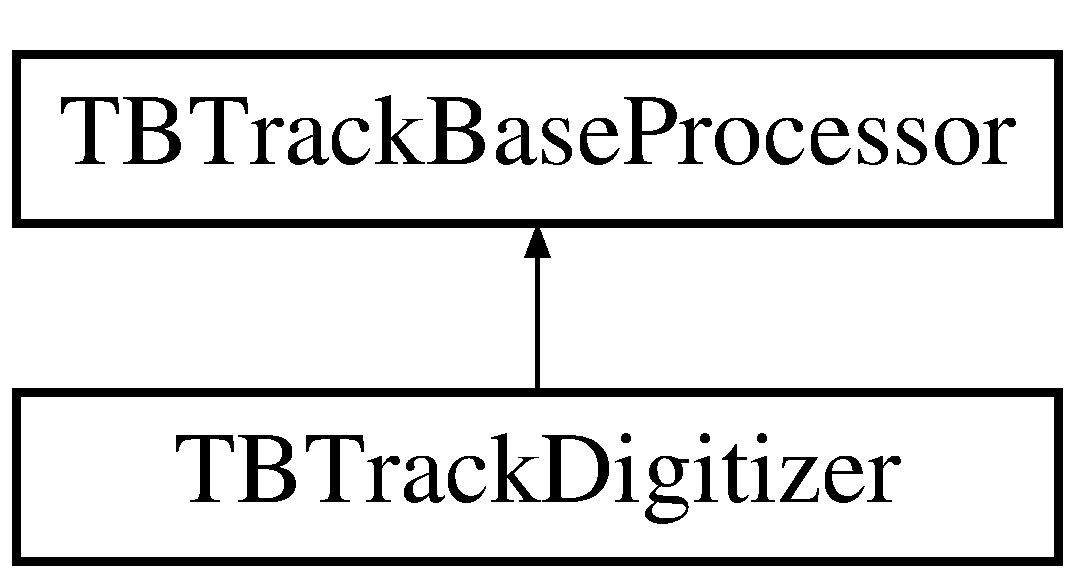
\includegraphics[height=2.000000cm]{classTBTrackDigitizer}
\end{center}
\end{figure}
\subsection*{Public Member Functions}
\begin{DoxyCompactItemize}
\item 
Processor $\ast$ {\bfseries new\-Processor} ()\label{classTBTrackDigitizer_a9b01b1d99677e61a302f5062511fdf03}

\item 
void {\bf Init} ()
\begin{DoxyCompactList}\small\item\em Called at the begin of the job before anything is read. \end{DoxyCompactList}\item 
void {\bf Process\-Run\-Header} (L\-C\-Run\-Header $\ast$run)
\begin{DoxyCompactList}\small\item\em Called for every run, e.\-g. \end{DoxyCompactList}\item 
void {\bf Process\-Event} (L\-C\-Event $\ast$evt\-P)\label{classTBTrackDigitizer_a026ff71a374a92b9f6ace5b858273896}

\begin{DoxyCompactList}\small\item\em Called for every event. \end{DoxyCompactList}\item 
void {\bfseries End} ()\label{classTBTrackDigitizer_a0a87ca69cc91c18f86b8f980c5b4e793}

\end{DoxyCompactItemize}
\subsection*{Protected Attributes}
\begin{DoxyCompactItemize}
\item 
std\-::string {\bf \-\_\-dc1\-Col\-Name}
\begin{DoxyCompactList}\small\item\em name of the D\-C1 collection (parameter). \end{DoxyCompactList}\item 
std\-::string {\bf \-\_\-dc2\-Col\-Name}
\begin{DoxyCompactList}\small\item\em name of the D\-C2 collection (parameter). \end{DoxyCompactList}\item 
std\-::string {\bf \-\_\-dc3\-Col\-Name}
\begin{DoxyCompactList}\small\item\em name of the D\-C3 collection (parameter). \end{DoxyCompactList}\item 
std\-::string {\bf \-\_\-dc4\-Col\-Name}
\begin{DoxyCompactList}\small\item\em name of the D\-C4 collection (parameter). \end{DoxyCompactList}\item 
std\-::string {\bf \-\_\-tracker\-Hit\-Col\-Name}
\begin{DoxyCompactList}\small\item\em if not empty a tracker hit collection of this name is added to the event. \end{DoxyCompactList}\item 
std\-::string {\bf \-\_\-\-T\-R\-U\-E\-Tracker\-Hit\-Col\-Name}
\begin{DoxyCompactList}\small\item\em if not empty a tracker hit collection of this name is added to the event. \end{DoxyCompactList}\end{DoxyCompactItemize}
\subsection*{Private Attributes}
\begin{DoxyCompactItemize}
\item 
int {\bfseries \-\_\-separate\-Hits\-X\-Y}\label{classTBTrackDigitizer_a61155291cafa45d49005249498b45735}

\end{DoxyCompactItemize}


\subsection{Detailed Description}


Definition at line 65 of file T\-B\-Track\-Digitizer.\-hh.



\subsection{Member Function Documentation}
\index{T\-B\-Track\-Digitizer@{T\-B\-Track\-Digitizer}!Init@{Init}}
\index{Init@{Init}!TBTrackDigitizer@{T\-B\-Track\-Digitizer}}
\subsubsection[{Init}]{\setlength{\rightskip}{0pt plus 5cm}void T\-B\-Track\-Digitizer\-::\-Init (
\begin{DoxyParamCaption}
{}
\end{DoxyParamCaption}
)\hspace{0.3cm}{\ttfamily [inline]}}\label{classTBTrackDigitizer_a6132a08eda7102d6bfae4a078334385e}


Called at the begin of the job before anything is read. 

Use to initialize the processor, e.\-g. book histograms. 

Definition at line 77 of file T\-B\-Track\-Digitizer.\-hh.

\index{T\-B\-Track\-Digitizer@{T\-B\-Track\-Digitizer}!Process\-Run\-Header@{Process\-Run\-Header}}
\index{Process\-Run\-Header@{Process\-Run\-Header}!TBTrackDigitizer@{T\-B\-Track\-Digitizer}}
\subsubsection[{Process\-Run\-Header}]{\setlength{\rightskip}{0pt plus 5cm}void T\-B\-Track\-Digitizer\-::\-Process\-Run\-Header (
\begin{DoxyParamCaption}
\item[{L\-C\-Run\-Header $\ast$}]{run}
\end{DoxyParamCaption}
)\hspace{0.3cm}{\ttfamily [inline]}}\label{classTBTrackDigitizer_a6cbdd55dcd60a0c1e20af931dd2bc102}


Called for every run, e.\-g. 

overwrite to initialize run dependent histograms. 

Definition at line 82 of file T\-B\-Track\-Digitizer.\-hh.



\subsection{Field Documentation}
\index{T\-B\-Track\-Digitizer@{T\-B\-Track\-Digitizer}!\-\_\-dc1\-Col\-Name@{\-\_\-dc1\-Col\-Name}}
\index{\-\_\-dc1\-Col\-Name@{\-\_\-dc1\-Col\-Name}!TBTrackDigitizer@{T\-B\-Track\-Digitizer}}
\subsubsection[{\-\_\-dc1\-Col\-Name}]{\setlength{\rightskip}{0pt plus 5cm}std\-::string T\-B\-Track\-Digitizer\-::\-\_\-dc1\-Col\-Name\hspace{0.3cm}{\ttfamily [protected]}}\label{classTBTrackDigitizer_ac1c60667782d5da7c3133fb8bc2a0fe6}


name of the D\-C1 collection (parameter). 



Definition at line 93 of file T\-B\-Track\-Digitizer.\-hh.

\index{T\-B\-Track\-Digitizer@{T\-B\-Track\-Digitizer}!\-\_\-dc2\-Col\-Name@{\-\_\-dc2\-Col\-Name}}
\index{\-\_\-dc2\-Col\-Name@{\-\_\-dc2\-Col\-Name}!TBTrackDigitizer@{T\-B\-Track\-Digitizer}}
\subsubsection[{\-\_\-dc2\-Col\-Name}]{\setlength{\rightskip}{0pt plus 5cm}std\-::string T\-B\-Track\-Digitizer\-::\-\_\-dc2\-Col\-Name\hspace{0.3cm}{\ttfamily [protected]}}\label{classTBTrackDigitizer_a072d9fc3b2b51490f107f92c08cfd583}


name of the D\-C2 collection (parameter). 



Definition at line 94 of file T\-B\-Track\-Digitizer.\-hh.

\index{T\-B\-Track\-Digitizer@{T\-B\-Track\-Digitizer}!\-\_\-dc3\-Col\-Name@{\-\_\-dc3\-Col\-Name}}
\index{\-\_\-dc3\-Col\-Name@{\-\_\-dc3\-Col\-Name}!TBTrackDigitizer@{T\-B\-Track\-Digitizer}}
\subsubsection[{\-\_\-dc3\-Col\-Name}]{\setlength{\rightskip}{0pt plus 5cm}std\-::string T\-B\-Track\-Digitizer\-::\-\_\-dc3\-Col\-Name\hspace{0.3cm}{\ttfamily [protected]}}\label{classTBTrackDigitizer_a371d605e218ee547903748baab348c60}


name of the D\-C3 collection (parameter). 



Definition at line 95 of file T\-B\-Track\-Digitizer.\-hh.

\index{T\-B\-Track\-Digitizer@{T\-B\-Track\-Digitizer}!\-\_\-dc4\-Col\-Name@{\-\_\-dc4\-Col\-Name}}
\index{\-\_\-dc4\-Col\-Name@{\-\_\-dc4\-Col\-Name}!TBTrackDigitizer@{T\-B\-Track\-Digitizer}}
\subsubsection[{\-\_\-dc4\-Col\-Name}]{\setlength{\rightskip}{0pt plus 5cm}std\-::string T\-B\-Track\-Digitizer\-::\-\_\-dc4\-Col\-Name\hspace{0.3cm}{\ttfamily [protected]}}\label{classTBTrackDigitizer_af81e1cc15ed1b7a95601f4531e0407e2}


name of the D\-C4 collection (parameter). 



Definition at line 96 of file T\-B\-Track\-Digitizer.\-hh.

\index{T\-B\-Track\-Digitizer@{T\-B\-Track\-Digitizer}!\-\_\-tracker\-Hit\-Col\-Name@{\-\_\-tracker\-Hit\-Col\-Name}}
\index{\-\_\-tracker\-Hit\-Col\-Name@{\-\_\-tracker\-Hit\-Col\-Name}!TBTrackDigitizer@{T\-B\-Track\-Digitizer}}
\subsubsection[{\-\_\-tracker\-Hit\-Col\-Name}]{\setlength{\rightskip}{0pt plus 5cm}std\-::string T\-B\-Track\-Digitizer\-::\-\_\-tracker\-Hit\-Col\-Name\hspace{0.3cm}{\ttfamily [protected]}}\label{classTBTrackDigitizer_a89170451358f13de1fb6391f8c16e3be}


if not empty a tracker hit collection of this name is added to the event. 



Definition at line 97 of file T\-B\-Track\-Digitizer.\-hh.

\index{T\-B\-Track\-Digitizer@{T\-B\-Track\-Digitizer}!\-\_\-\-T\-R\-U\-E\-Tracker\-Hit\-Col\-Name@{\-\_\-\-T\-R\-U\-E\-Tracker\-Hit\-Col\-Name}}
\index{\-\_\-\-T\-R\-U\-E\-Tracker\-Hit\-Col\-Name@{\-\_\-\-T\-R\-U\-E\-Tracker\-Hit\-Col\-Name}!TBTrackDigitizer@{T\-B\-Track\-Digitizer}}
\subsubsection[{\-\_\-\-T\-R\-U\-E\-Tracker\-Hit\-Col\-Name}]{\setlength{\rightskip}{0pt plus 5cm}std\-::string T\-B\-Track\-Digitizer\-::\-\_\-\-T\-R\-U\-E\-Tracker\-Hit\-Col\-Name\hspace{0.3cm}{\ttfamily [protected]}}\label{classTBTrackDigitizer_a05101ed4c3f17c4c75b6386eab702b39}


if not empty a tracker hit collection of this name is added to the event. 



Definition at line 98 of file T\-B\-Track\-Digitizer.\-hh.



The documentation for this class was generated from the following file\-:\begin{DoxyCompactItemize}
\item 
T\-B\-Track\-Digitizer.\-hh\end{DoxyCompactItemize}

\section{digisim\-:\-:Tcmt\-Crosstalk Class Reference}
\label{classdigisim_1_1TcmtCrosstalk}\index{digisim\-::\-Tcmt\-Crosstalk@{digisim\-::\-Tcmt\-Crosstalk}}
Inheritance diagram for digisim\-:\-:Tcmt\-Crosstalk\-:\begin{figure}[H]
\begin{center}
\leavevmode
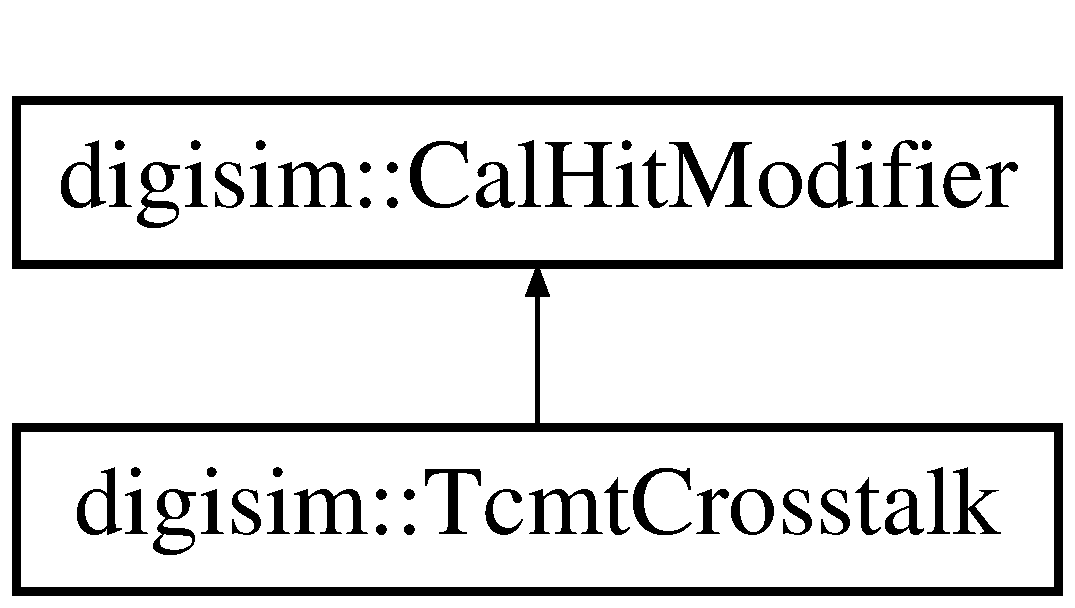
\includegraphics[height=2.000000cm]{classdigisim_1_1TcmtCrosstalk}
\end{center}
\end{figure}
\subsection*{Public Member Functions}
\begin{DoxyCompactItemize}
\item 
{\bf Tcmt\-Crosstalk} $\ast$ {\bfseries new\-Instance} (const std\-::string \&mod\-Name)\label{classdigisim_1_1TcmtCrosstalk_a0cec6dfca13d00791a0aaad3271f5739}

\item 
void {\bfseries init} (std\-::vector$<$ float $>$ \&floats)\label{classdigisim_1_1TcmtCrosstalk_a68c9d3d0aacc848ce0257df9c795d552}

\item 
void {\bfseries process\-Hits} (Temp\-Cal\-Hit\-Map \&hitmap)\label{classdigisim_1_1TcmtCrosstalk_af58027092df6d4082b99ea5fc6046cb2}

\item 
void {\bfseries print} () const \label{classdigisim_1_1TcmtCrosstalk_adb647c962aae704cd31c767fcf78532a}

\end{DoxyCompactItemize}
\subsection*{Private Member Functions}
\begin{DoxyCompactItemize}
\item 
{\bfseries Tcmt\-Crosstalk} (const std\-::string \&mod\-Name)\label{classdigisim_1_1TcmtCrosstalk_aa596f349686f6ab1e96e1fdfcaf43dd1}

\item 
{\bfseries Tcmt\-Crosstalk} (const {\bf Tcmt\-Crosstalk} \&rhs)\label{classdigisim_1_1TcmtCrosstalk_adbbdc315429667a84499815e415c845c}

\end{DoxyCompactItemize}
\subsection*{Private Attributes}
\begin{DoxyCompactItemize}
\item 
std\-::vector$<$ float $>$ {\bfseries \-\_\-par}\label{classdigisim_1_1TcmtCrosstalk_ad2c79f9d6a2f613133a7ac6aa29c74e4}

\end{DoxyCompactItemize}
\subsection*{Additional Inherited Members}


\subsection{Detailed Description}


Definition at line 19 of file Tcmt\-Crosstalk.\-hpp.



The documentation for this class was generated from the following files\-:\begin{DoxyCompactItemize}
\item 
Tcmt\-Crosstalk.\-hpp\item 
Tcmt\-Crosstalk.\-cpp\end{DoxyCompactItemize}

\section{digisim\-:\-:Tcmt\-Ganging\-Modifier Class Reference}
\label{classdigisim_1_1TcmtGangingModifier}\index{digisim\-::\-Tcmt\-Ganging\-Modifier@{digisim\-::\-Tcmt\-Ganging\-Modifier}}
Inheritance diagram for digisim\-:\-:Tcmt\-Ganging\-Modifier\-:\begin{figure}[H]
\begin{center}
\leavevmode
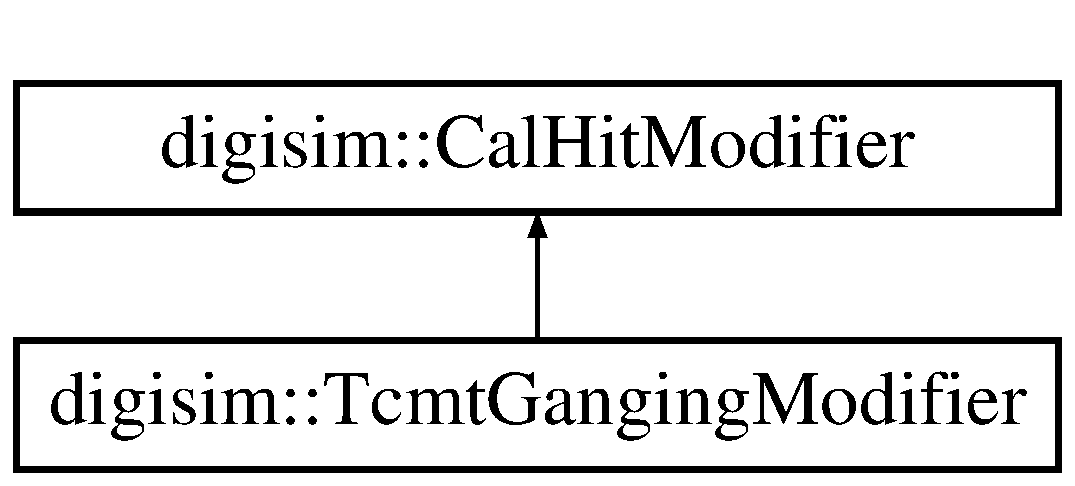
\includegraphics[height=2.000000cm]{classdigisim_1_1TcmtGangingModifier}
\end{center}
\end{figure}
\subsection*{Public Member Functions}
\begin{DoxyCompactItemize}
\item 
{\bf Tcmt\-Ganging\-Modifier} $\ast$ {\bfseries new\-Instance} (const std\-::string \&mod\-Name)\label{classdigisim_1_1TcmtGangingModifier_aca7031b84d348b2886405a8df0afddd4}

\item 
void {\bfseries init} (std\-::vector$<$ float $>$ \&floats)\label{classdigisim_1_1TcmtGangingModifier_a6d8d930b887ed576ce520f77e57a37d6}

\item 
void {\bfseries process\-Hits} (Temp\-Cal\-Hit\-Map \&hitmap)\label{classdigisim_1_1TcmtGangingModifier_afe4c5cdff1af6d08a62e3922d6be774c}

\item 
void {\bfseries print} () const \label{classdigisim_1_1TcmtGangingModifier_ac0ad1555a9bb4508ccdb07452507fee3}

\end{DoxyCompactItemize}
\subsection*{Private Member Functions}
\begin{DoxyCompactItemize}
\item 
{\bf Tcmt\-Ganging\-Modifier} (const std\-::string \&mod\-Name)\label{classdigisim_1_1TcmtGangingModifier_a227a5c12000f9b5a6342c3b65c4870e9}

\begin{DoxyCompactList}\small\item\em Called after data processing for clean up. \end{DoxyCompactList}\item 
{\bfseries Tcmt\-Ganging\-Modifier} (const {\bf Tcmt\-Ganging\-Modifier} \&rhs)\label{classdigisim_1_1TcmtGangingModifier_a3d2dc1562cdf7ebb894b6ec3b1aeb396}

\end{DoxyCompactItemize}
\subsection*{Private Attributes}
\begin{DoxyCompactItemize}
\item 
std\-::vector$<$ float $>$ {\bfseries \-\_\-par}\label{classdigisim_1_1TcmtGangingModifier_ac8333fe6c9ef5c4570da91cc968b1b84}

\end{DoxyCompactItemize}
\subsection*{Additional Inherited Members}


\subsection{Detailed Description}


Definition at line 19 of file Tcmt\-Ganging\-Modifier.\-hpp.



The documentation for this class was generated from the following files\-:\begin{DoxyCompactItemize}
\item 
Tcmt\-Ganging\-Modifier.\-hpp\item 
Tcmt\-Ganging\-Modifier.\-cpp\end{DoxyCompactItemize}

\section{digisim\-:\-:Temp\-Cal\-Hit Class Reference}
\label{classdigisim_1_1TempCalHit}\index{digisim\-::\-Temp\-Cal\-Hit@{digisim\-::\-Temp\-Cal\-Hit}}
\subsection*{Public Member Functions}
\begin{DoxyCompactItemize}
\item 
{\bfseries Temp\-Cal\-Hit} (const {\bf Temp\-Cal\-Hit} \&oldhit)\label{classdigisim_1_1TempCalHit_a271161b6232b82537a902e6d4958b54b}

\item 
{\bfseries Temp\-Cal\-Hit} (long long simid, double energy, double time)\label{classdigisim_1_1TempCalHit_ac670c4dd69d12601c76a86dbf1b1ebe0}

\item 
{\bfseries Temp\-Cal\-Hit} (long long rawid, long long simid, double energy, double time)\label{classdigisim_1_1TempCalHit_afcd10b7f0af31bce55a84c1c7471b554}

\item 
{\bf Temp\-Cal\-Hit} \& {\bfseries operator=} (const {\bf Temp\-Cal\-Hit} \&rhs)\label{classdigisim_1_1TempCalHit_a44a283e875c81b62823b8c907f39b6fb}

\item 
double {\bfseries get\-Total\-Energy} () const \label{classdigisim_1_1TempCalHit_a04262c7202fa8ca7a9e72a6e8bc0a53a}

\item 
void {\bf scale\-Energy} (double factor)
\begin{DoxyCompactList}\small\item\em Scales the global energy. \end{DoxyCompactList}\item 
void {\bf set\-Energy} (double energy)
\begin{DoxyCompactList}\small\item\em Changes global energy. \end{DoxyCompactList}\item 
void {\bf set\-Time} (double tstamp)\label{classdigisim_1_1TempCalHit_afb7c3c822364aab663608bad1dbfe226}

\begin{DoxyCompactList}\small\item\em Changes global time stamp -- use it with care, as it then becomes different than the timings of any individual contribution. \end{DoxyCompactList}\item 
double {\bf get\-Primary\-Time} () const 
\begin{DoxyCompactList}\small\item\em Primary time\-: either earliest time or time from largest contribution. \end{DoxyCompactList}\item 
void {\bf add\-Contribution} (long long id, double energy, double time)\label{classdigisim_1_1TempCalHit_ad788245a99a8cfdd8945b199453eb7cc}

\begin{DoxyCompactList}\small\item\em Add a contribution from a simulated hit. \end{DoxyCompactList}\item 
std\-::map$<$ long long, {\bf Hit\-Contrib} $>$ \& {\bf get\-Contributions} ()
\begin{DoxyCompactList}\small\item\em Reduce contribution from original hit, due to crosstalk into neighbors. \end{DoxyCompactList}\item 
std\-::vector$<$ double $>$ {\bf get\-Energy\-Contributions} () const \label{classdigisim_1_1TempCalHit_ae952b984ab633fc57b8c0a9e70f0a23c}

\begin{DoxyCompactList}\small\item\em Return a vector with the energy contributions to the current \doxyref{Temp\-Cal\-Hit}{p.}{classdigisim_1_1TempCalHit}. \end{DoxyCompactList}\item 
std\-::vector$<$ long long $>$ {\bf get\-Contributing\-I\-Ds} () const \label{classdigisim_1_1TempCalHit_a87910d2e8b1dad1bb6cd85c390c5b898}

\begin{DoxyCompactList}\small\item\em Return a vector with the Cell\-I\-Ds for the sim hits' contributions to the current \doxyref{Temp\-Cal\-Hit}{p.}{classdigisim_1_1TempCalHit}. \end{DoxyCompactList}\item 
void {\bf set\-Cell\-I\-D0} (int id)\label{classdigisim_1_1TempCalHit_ab797d361b09b92b40e4798daa451cd74}

\begin{DoxyCompactList}\small\item\em Set cell I\-D. \end{DoxyCompactList}\item 
void {\bfseries set\-Cell\-I\-D1} (int id)\label{classdigisim_1_1TempCalHit_a65e2ec838bc20536a10b55088f8e3a13}

\item 
void {\bfseries set\-Cell\-I\-D} (long long id)\label{classdigisim_1_1TempCalHit_ab247e1d0aeffd428cafdf05c548cbe18}

\item 
int {\bfseries get\-Cell\-I\-D0} () const \label{classdigisim_1_1TempCalHit_a13184fc7d8f925e9678060228b0b7c00}

\item 
int {\bfseries get\-Cell\-I\-D1} () const \label{classdigisim_1_1TempCalHit_a5a739e1185c043c2228d3ac2dec5e9de}

\item 
int {\bfseries get\-Cell\-I\-D} () const \label{classdigisim_1_1TempCalHit_aa2bd295569484bb8e19111f9c98ca1b1}

\end{DoxyCompactItemize}
\subsection*{Private Member Functions}
\begin{DoxyCompactItemize}
\item 
int {\bfseries find\-Contribution} (long long cell\-I\-D)\label{classdigisim_1_1TempCalHit_a3cec54c73b27fae1f283c827a882f978}

\end{DoxyCompactItemize}
\subsection*{Private Attributes}
\begin{DoxyCompactItemize}
\item 
long long {\bfseries \-\_\-raw\-I\-D}\label{classdigisim_1_1TempCalHit_ab6edba9f8e1f298a62f7068f80c1d674}

\item 
double {\bfseries \-\_\-energy}\label{classdigisim_1_1TempCalHit_a5cabc532b09aab664222dabd1b030a6e}

\item 
double {\bfseries \-\_\-time}\label{classdigisim_1_1TempCalHit_a7d8fc80100e8517f9e982ec3721626d1}

\item 
std\-::map$<$ long long, {\bf Hit\-Contrib} $>$ $\ast$ {\bfseries \-\_\-sim\-Hits}\label{classdigisim_1_1TempCalHit_a2014cf473a8b9bbf5ff6c3cc5b3f8bee}

\item 
std\-::vector$<$ {\bf Hit\-Contrib} $>$\\*
\-::const\-\_\-iterator {\bfseries i}\label{classdigisim_1_1TempCalHit_a84599798fa4c195cb77377896f66fb18}

\end{DoxyCompactItemize}


\subsection{Detailed Description}


Definition at line 13 of file Temp\-Cal\-Hit.\-hpp.



\subsection{Member Function Documentation}
\index{digisim\-::\-Temp\-Cal\-Hit@{digisim\-::\-Temp\-Cal\-Hit}!get\-Contributions@{get\-Contributions}}
\index{get\-Contributions@{get\-Contributions}!digisim::TempCalHit@{digisim\-::\-Temp\-Cal\-Hit}}
\subsubsection[{get\-Contributions}]{\setlength{\rightskip}{0pt plus 5cm}map$<$ long long, {\bf Hit\-Contrib} $>$ \& digisim\-::\-Temp\-Cal\-Hit\-::get\-Contributions (
\begin{DoxyParamCaption}
{}
\end{DoxyParamCaption}
)}\label{classdigisim_1_1TempCalHit_aaca7f61fde5340882bbd8d626a54715f}


Reduce contribution from original hit, due to crosstalk into neighbors. 

Return the contributions from simulated hits to the current \doxyref{Temp\-Cal\-Hit}{p.}{classdigisim_1_1TempCalHit} 

Definition at line 160 of file Temp\-Cal\-Hit.\-cpp.

\index{digisim\-::\-Temp\-Cal\-Hit@{digisim\-::\-Temp\-Cal\-Hit}!get\-Primary\-Time@{get\-Primary\-Time}}
\index{get\-Primary\-Time@{get\-Primary\-Time}!digisim::TempCalHit@{digisim\-::\-Temp\-Cal\-Hit}}
\subsubsection[{get\-Primary\-Time}]{\setlength{\rightskip}{0pt plus 5cm}double digisim\-::\-Temp\-Cal\-Hit\-::get\-Primary\-Time (
\begin{DoxyParamCaption}
{}
\end{DoxyParamCaption}
) const}\label{classdigisim_1_1TempCalHit_a137d416587c18c83d58592502316e7dd}


Primary time\-: either earliest time or time from largest contribution. 

It is currently set as the earliest time. 

Definition at line 121 of file Temp\-Cal\-Hit.\-cpp.



Referenced by digisim\-::\-Smeared\-Timing\-::transform\-Time().

\index{digisim\-::\-Temp\-Cal\-Hit@{digisim\-::\-Temp\-Cal\-Hit}!scale\-Energy@{scale\-Energy}}
\index{scale\-Energy@{scale\-Energy}!digisim::TempCalHit@{digisim\-::\-Temp\-Cal\-Hit}}
\subsubsection[{scale\-Energy}]{\setlength{\rightskip}{0pt plus 5cm}void digisim\-::\-Temp\-Cal\-Hit\-::scale\-Energy (
\begin{DoxyParamCaption}
\item[{double}]{factor}
\end{DoxyParamCaption}
)}\label{classdigisim_1_1TempCalHit_ad4bdc1b03a6cfa99feb5e1538683f782}


Scales the global energy. 

This changes the energy of each contribution by the same factor. 
\begin{DoxyParams}{Parameters}
{\em factor} & Applied to each contribution separately \\
\hline
\end{DoxyParams}


Definition at line 94 of file Temp\-Cal\-Hit.\-cpp.



Referenced by set\-Energy().

\index{digisim\-::\-Temp\-Cal\-Hit@{digisim\-::\-Temp\-Cal\-Hit}!set\-Energy@{set\-Energy}}
\index{set\-Energy@{set\-Energy}!digisim::TempCalHit@{digisim\-::\-Temp\-Cal\-Hit}}
\subsubsection[{set\-Energy}]{\setlength{\rightskip}{0pt plus 5cm}void digisim\-::\-Temp\-Cal\-Hit\-::set\-Energy (
\begin{DoxyParamCaption}
\item[{double}]{energy}
\end{DoxyParamCaption}
)}\label{classdigisim_1_1TempCalHit_a5cbad6a81917f7c511526dc6012b6f3e}


Changes global energy. 

Actually, this changes the energy of each contribution by the same factor, so that final energy gets updated to the value provided. 
\begin{DoxyParams}{Parameters}
{\em energy} & Final value of total energy \\
\hline
\end{DoxyParams}


Definition at line 101 of file Temp\-Cal\-Hit.\-cpp.



References scale\-Energy().



The documentation for this class was generated from the following files\-:\begin{DoxyCompactItemize}
\item 
Temp\-Cal\-Hit.\-hpp\item 
Temp\-Cal\-Hit.\-cpp\end{DoxyCompactItemize}

\section{temp\-G\-E\-A\-Rvariables Class Reference}
\label{classtempGEARvariables}\index{temp\-G\-E\-A\-Rvariables@{temp\-G\-E\-A\-Rvariables}}
\subsection*{Public Member Functions}
\begin{DoxyCompactItemize}
\item 
{\bfseries temp\-G\-E\-A\-Rvariables} (int Symmetry\-Order)\label{classtempGEARvariables_a57255f8d771b18a8bd5e5875503086fa}

\end{DoxyCompactItemize}
\subsection*{Data Fields}
\begin{DoxyCompactItemize}
\item 
int {\bf nlayers}\label{classtempGEARvariables_ae0477b8ff1f6593407a77095c2827a4a}

\begin{DoxyCompactList}\small\item\em Symmetry\-Order is the order of the rotational symmetry \par
 8 for an octagonal barrel calorimeter\par
 2 for an endcap calorimeter\par
 1 for a standalone prototype\par
 0 for an idealized cylindrical calorimeter. \end{DoxyCompactList}\item 
int {\bfseries n\-Wafer0}\label{classtempGEARvariables_ad6b0630d8d0e1c5ffec7a196b1a6331a}

\item 
int {\bfseries n\-Wafer1}\label{classtempGEARvariables_ab46b808b0c93323c3b09b30ddfcdbedb}

\item 
int {\bfseries n\-Cellper\-Wafer0}\label{classtempGEARvariables_a77c909e9e84990cea2f2213e2202a37e}

\item 
int {\bfseries n\-Cellper\-Wafer1}\label{classtempGEARvariables_a4b93cd0c376a260363108092ca5fb83c}

\item 
bool {\bfseries use\-Encoder32}\label{classtempGEARvariables_a31918a949ac9be7ab94ccaca8fa58056}

\end{DoxyCompactItemize}


\subsection{Detailed Description}


Definition at line 4 of file temp\-G\-E\-A\-Rvariables.\-hpp.



The documentation for this class was generated from the following file\-:\begin{DoxyCompactItemize}
\item 
temp\-G\-E\-A\-Rvariables.\-hpp\end{DoxyCompactItemize}

\section{C\-A\-L\-I\-C\-E\-:\-:tokyo\-\_\-layer Class Reference}
\label{classCALICE_1_1tokyo__layer}\index{C\-A\-L\-I\-C\-E\-::tokyo\-\_\-layer@{C\-A\-L\-I\-C\-E\-::tokyo\-\_\-layer}}


Implementation of ganger in T\-O\-K\-Y\-O Layer.  


Inheritance diagram for C\-A\-L\-I\-C\-E\-:\-:tokyo\-\_\-layer\-:\begin{figure}[H]
\begin{center}
\leavevmode
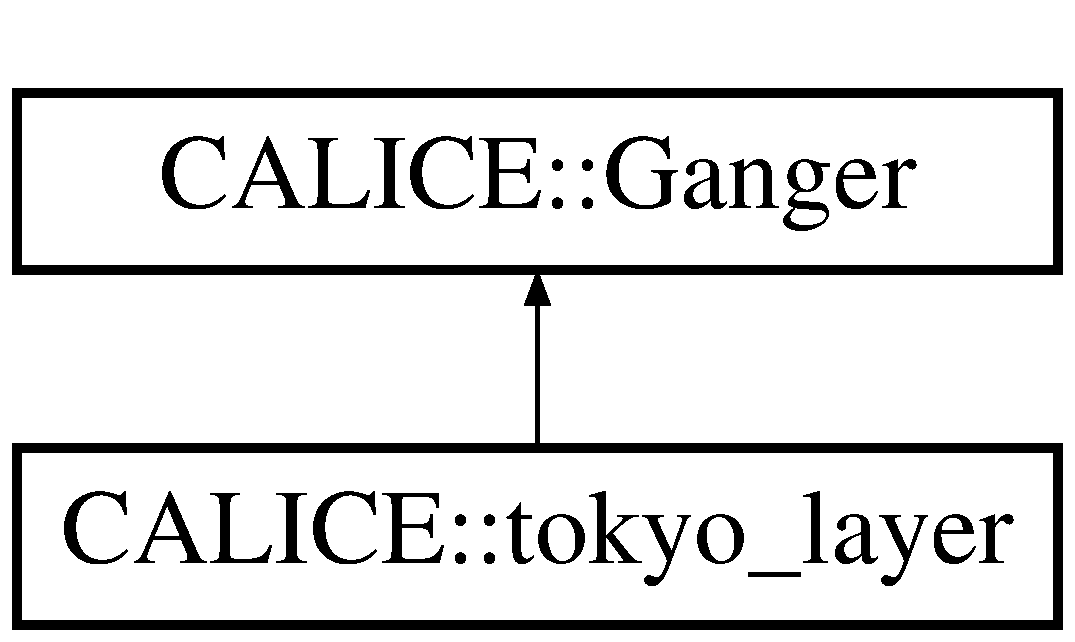
\includegraphics[height=2.000000cm]{classCALICE_1_1tokyo__layer}
\end{center}
\end{figure}
\subsection*{Public Member Functions}
\begin{DoxyCompactItemize}
\item 
{\bfseries tokyo\-\_\-layer} ({\bf Contribution\-Map} $\ast$cm, float factor)\label{classCALICE_1_1tokyo__layer_ae59ee4b18714f84f8fb57e9386721757}

\item 
bool {\bf responsible} ({\bf geometrical\-Indices} indices)\label{classCALICE_1_1tokyo__layer_af2110fc66083f23ae7baac020ddd1f37}

\begin{DoxyCompactList}\small\item\em Implementations have to implement where in I/\-J they are responsible. \end{DoxyCompactList}\end{DoxyCompactItemize}


\subsection{Detailed Description}
Implementation of ganger in T\-O\-K\-Y\-O Layer. 

Definition at line 64 of file Ahc2\-Ganging\-Processor.\-cc.



The documentation for this class was generated from the following file\-:\begin{DoxyCompactItemize}
\item 
Ahc2\-Ganging\-Processor.\-cc\end{DoxyCompactItemize}

\section{top\-Both Class Reference}
\label{classtopBoth}\index{top\-Both@{top\-Both}}


Implementation of ganger.  


Inheritance diagram for top\-Both\-:\begin{figure}[H]
\begin{center}
\leavevmode
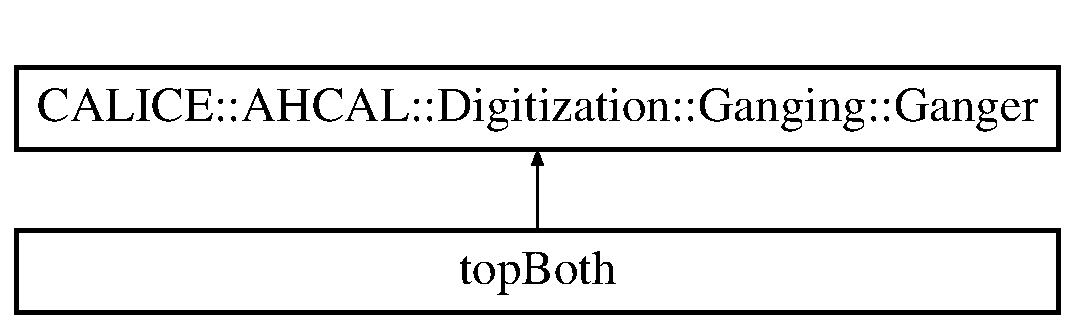
\includegraphics[height=2.000000cm]{classtopBoth}
\end{center}
\end{figure}
\subsection*{Public Member Functions}
\begin{DoxyCompactItemize}
\item 
{\bfseries top\-Both} ({\bf Contribution\-Map} $\ast$cm, float factor)\label{classtopBoth_a25f74b3d955a26ade7d58df706ed3a8a}

\item 
bool {\bf responsible} ({\bf Geometrical\-Indices} indices)\label{classtopBoth_a4772fca3483764c3b5469f020f1c9f26}

\begin{DoxyCompactList}\small\item\em Implementations have to implement where in I/\-J they are responsible. \end{DoxyCompactList}\end{DoxyCompactItemize}


\subsection{Detailed Description}
Implementation of ganger. 

Definition at line 100 of file ahcal\-Ganging\-Processor.\-cc.



The documentation for this class was generated from the following file\-:\begin{DoxyCompactItemize}
\item 
ahcal\-Ganging\-Processor.\-cc\end{DoxyCompactItemize}

%--- End generated contents ---

% Index
\newpage
\phantomsection
\addcontentsline{toc}{part}{Index}
\printindex

\end{document}
